\documentclass[]{book}
\usepackage{lmodern}
\usepackage{amssymb,amsmath}
\usepackage{ifxetex,ifluatex}
\usepackage{fixltx2e} % provides \textsubscript
\ifnum 0\ifxetex 1\fi\ifluatex 1\fi=0 % if pdftex
  \usepackage[T1]{fontenc}
  \usepackage[utf8]{inputenc}
\else % if luatex or xelatex
  \ifxetex
    \usepackage{mathspec}
  \else
    \usepackage{fontspec}
  \fi
  \defaultfontfeatures{Ligatures=TeX,Scale=MatchLowercase}
\fi
% use upquote if available, for straight quotes in verbatim environments
\IfFileExists{upquote.sty}{\usepackage{upquote}}{}
% use microtype if available
\IfFileExists{microtype.sty}{%
\usepackage{microtype}
\UseMicrotypeSet[protrusion]{basicmath} % disable protrusion for tt fonts
}{}
\usepackage{hyperref}
\hypersetup{unicode=true,
            pdftitle={数据分析残卷},
            pdfauthor={于淼},
            pdfborder={0 0 0},
            breaklinks=true}
\urlstyle{same}  % don't use monospace font for urls
\usepackage{natbib}
\bibliographystyle{apalike}
\usepackage{color}
\usepackage{fancyvrb}
\newcommand{\VerbBar}{|}
\newcommand{\VERB}{\Verb[commandchars=\\\{\}]}
\DefineVerbatimEnvironment{Highlighting}{Verbatim}{commandchars=\\\{\}}
% Add ',fontsize=\small' for more characters per line
\usepackage{framed}
\definecolor{shadecolor}{RGB}{248,248,248}
\newenvironment{Shaded}{\begin{snugshade}}{\end{snugshade}}
\newcommand{\AlertTok}[1]{\textcolor[rgb]{0.94,0.16,0.16}{#1}}
\newcommand{\AnnotationTok}[1]{\textcolor[rgb]{0.56,0.35,0.01}{\textbf{\textit{#1}}}}
\newcommand{\AttributeTok}[1]{\textcolor[rgb]{0.77,0.63,0.00}{#1}}
\newcommand{\BaseNTok}[1]{\textcolor[rgb]{0.00,0.00,0.81}{#1}}
\newcommand{\BuiltInTok}[1]{#1}
\newcommand{\CharTok}[1]{\textcolor[rgb]{0.31,0.60,0.02}{#1}}
\newcommand{\CommentTok}[1]{\textcolor[rgb]{0.56,0.35,0.01}{\textit{#1}}}
\newcommand{\CommentVarTok}[1]{\textcolor[rgb]{0.56,0.35,0.01}{\textbf{\textit{#1}}}}
\newcommand{\ConstantTok}[1]{\textcolor[rgb]{0.00,0.00,0.00}{#1}}
\newcommand{\ControlFlowTok}[1]{\textcolor[rgb]{0.13,0.29,0.53}{\textbf{#1}}}
\newcommand{\DataTypeTok}[1]{\textcolor[rgb]{0.13,0.29,0.53}{#1}}
\newcommand{\DecValTok}[1]{\textcolor[rgb]{0.00,0.00,0.81}{#1}}
\newcommand{\DocumentationTok}[1]{\textcolor[rgb]{0.56,0.35,0.01}{\textbf{\textit{#1}}}}
\newcommand{\ErrorTok}[1]{\textcolor[rgb]{0.64,0.00,0.00}{\textbf{#1}}}
\newcommand{\ExtensionTok}[1]{#1}
\newcommand{\FloatTok}[1]{\textcolor[rgb]{0.00,0.00,0.81}{#1}}
\newcommand{\FunctionTok}[1]{\textcolor[rgb]{0.00,0.00,0.00}{#1}}
\newcommand{\ImportTok}[1]{#1}
\newcommand{\InformationTok}[1]{\textcolor[rgb]{0.56,0.35,0.01}{\textbf{\textit{#1}}}}
\newcommand{\KeywordTok}[1]{\textcolor[rgb]{0.13,0.29,0.53}{\textbf{#1}}}
\newcommand{\NormalTok}[1]{#1}
\newcommand{\OperatorTok}[1]{\textcolor[rgb]{0.81,0.36,0.00}{\textbf{#1}}}
\newcommand{\OtherTok}[1]{\textcolor[rgb]{0.56,0.35,0.01}{#1}}
\newcommand{\PreprocessorTok}[1]{\textcolor[rgb]{0.56,0.35,0.01}{\textit{#1}}}
\newcommand{\RegionMarkerTok}[1]{#1}
\newcommand{\SpecialCharTok}[1]{\textcolor[rgb]{0.00,0.00,0.00}{#1}}
\newcommand{\SpecialStringTok}[1]{\textcolor[rgb]{0.31,0.60,0.02}{#1}}
\newcommand{\StringTok}[1]{\textcolor[rgb]{0.31,0.60,0.02}{#1}}
\newcommand{\VariableTok}[1]{\textcolor[rgb]{0.00,0.00,0.00}{#1}}
\newcommand{\VerbatimStringTok}[1]{\textcolor[rgb]{0.31,0.60,0.02}{#1}}
\newcommand{\WarningTok}[1]{\textcolor[rgb]{0.56,0.35,0.01}{\textbf{\textit{#1}}}}
\usepackage{longtable,booktabs}
\usepackage{graphicx,grffile}
\makeatletter
\def\maxwidth{\ifdim\Gin@nat@width>\linewidth\linewidth\else\Gin@nat@width\fi}
\def\maxheight{\ifdim\Gin@nat@height>\textheight\textheight\else\Gin@nat@height\fi}
\makeatother
% Scale images if necessary, so that they will not overflow the page
% margins by default, and it is still possible to overwrite the defaults
% using explicit options in \includegraphics[width, height, ...]{}
\setkeys{Gin}{width=\maxwidth,height=\maxheight,keepaspectratio}
\IfFileExists{parskip.sty}{%
\usepackage{parskip}
}{% else
\setlength{\parindent}{0pt}
\setlength{\parskip}{6pt plus 2pt minus 1pt}
}
\setlength{\emergencystretch}{3em}  % prevent overfull lines
\providecommand{\tightlist}{%
  \setlength{\itemsep}{0pt}\setlength{\parskip}{0pt}}
\setcounter{secnumdepth}{5}
% Redefines (sub)paragraphs to behave more like sections
\ifx\paragraph\undefined\else
\let\oldparagraph\paragraph
\renewcommand{\paragraph}[1]{\oldparagraph{#1}\mbox{}}
\fi
\ifx\subparagraph\undefined\else
\let\oldsubparagraph\subparagraph
\renewcommand{\subparagraph}[1]{\oldsubparagraph{#1}\mbox{}}
\fi

%%% Use protect on footnotes to avoid problems with footnotes in titles
\let\rmarkdownfootnote\footnote%
\def\footnote{\protect\rmarkdownfootnote}

%%% Change title format to be more compact
\usepackage{titling}

% Create subtitle command for use in maketitle
\providecommand{\subtitle}[1]{
  \posttitle{
    \begin{center}\large#1\end{center}
    }
}

\setlength{\droptitle}{-2em}

  \title{数据分析残卷}
    \pretitle{\vspace{\droptitle}\centering\huge}
  \posttitle{\par}
    \author{于淼}
    \preauthor{\centering\large\emph}
  \postauthor{\par}
      \predate{\centering\large\emph}
  \postdate{\par}
    \date{2019-11-25}

\usepackage{booktabs}
\usepackage{xeCJK}
\setCJKmainfont[BoldFont=STZhongsong, ItalicFont=STKaiti]{STSong}
\setCJKsansfont[BoldFont=STHeiti]{STXihei}
\setCJKmonofont{STFangsong}\renewcommand{\chaptername}{章}
\usepackage{graphicx}
\usepackage{MnSymbol}

\begin{document}
\maketitle

{
\setcounter{tocdepth}{1}
\tableofcontents
}
\hypertarget{ux5e8f}{%
\chapter*{序}\label{ux5e8f}}
\addcontentsline{toc}{chapter}{序}

学习都是从模仿开始的,而模仿则意味着不加区别的接受,若是混口饭吃,自然也就够了,但模仿多了便能看到这知识表象下的东西。如果还能提炼一下,变成了自己的经验,各种经验互相联系影响,便有了理论。所以学习大都从知识点开始,而以形成一家之言为终,倘若这一家之言可以得到别人的认可,知识就开始传承了。且不论有多少东西会被反复发现发明出来,但是世界在某种程度上是可知的便是智慧生物生存的福利。

就数据分析而言,我自学过很多教材,可以说不同门派间手段差异非常大,但总又妄想一统江湖,所以便有了这份笔记来整合。不论最终的完成度如何,这都只会是一本残卷,因为这世界总有未知,也因此总有希望。

本书以\texttt{bookdown}写作,感谢相关工具开发者的努力,站在前人肩上看世界确实视角要开阔。

\hypertarget{intro}{%
\chapter{导论}\label{intro}}

\hypertarget{ux6570ux636eux79d1ux5b66}{%
\section{数据科学}\label{ux6570ux636eux79d1ux5b66}}

\begin{itemize}
\tightlist
\item
  核心:数据处理
\item
  研究对象:实际问题(跨学科)
\item
  方法:统计学 计算机科学 专业领域
\item
  数据科学家:

  \begin{itemize}
  \tightlist
  \item
    统计学水平高的程序员
  \item
    编程水平高的统计学家
  \item
    学术好奇心
  \item
    沟通交流能力
  \item
    产品经理
  \end{itemize}
\item
  数据次于问题
\item
  大数据依赖科学而不是数据
\item
  实验设计 重视可重复性随机与分组 预测与推断不同 不要选数据
\end{itemize}

\hypertarget{ux57faux672cux95eeux9898}{%
\section{基本问题}\label{ux57faux672cux95eeux9898}}

\begin{itemize}
\tightlist
\item
  描述分析:对数据进行描述但不解释
\item
  探索分析:寻找未知的变量间关系 (相关不代表因果)
\item
  推断分析:用小样本推断总体 统计模型的目标 强依赖采样过程
\item
  预测分析:用一组变量预测另一变量 不一定有因果关系
\item
  因果分析:改变一个变量引发另一个变量变化的分析 随机实验 平均效果
\item
  机理分析:对个体改变一个变量所导致另一个变量的精确变化 公式模拟与参数拟合
\end{itemize}

\hypertarget{ux5de5ux4f5cux6d41ux7a0b}{%
\section{工作流程}\label{ux5de5ux4f5cux6d41ux7a0b}}

\begin{itemize}
\tightlist
\item
  数据收集
\item
  数据整理
\item
  数据探索
\item
  数据建模
\item
  模型评价
\item
  结果交流
\end{itemize}

\hypertarget{ux6982ux7387ux4e0eux5206ux5e03}{%
\section{概率与分布}\label{ux6982ux7387ux4e0eux5206ux5e03}}

概率与分布是统计的基本世界观,当我们用概率来理解世界时,所有事物便不仅仅是此时此刻的事,而是可能性中的一种。这种全局观好比从上帝视角开启有限平行宇宙,即使你知道每种状态及其概率,最后结果也无法预判。

\begin{itemize}
\tightlist
\item
  从可能性到独立事件概率计算
\item
  从联合概率到条件概率到贝叶斯公式
\item
  事件的发生空间到分布
\item
  多事件发生概率比较到标准化分布-z值
\item
  正态分布评价拟合
\item
  贝努利分布
\item
  二项分布,固定总数,成功概率,二项分布可用正态分布近似求值,也可用二项分布取精确值,求区间概率要扩大
\item
  负二项分布,固定成功次数概率
\item
  几何分布,最后一次成功概率
\item
  超几何分布,不放回抽样,成功概率
\item
  泊松分布,实验次数多,概率小,发生概率,泊松过程
\end{itemize}

\hypertarget{ux7edfux8ba1ux91cf}{%
\section{统计量}\label{ux7edfux8ba1ux91cf}}

统计量是对样本性质的一种描述或简化,用来提取设计者所关注的信号并尽可能排除掉噪音。

\begin{itemize}
\item
  总体到样本

  \begin{itemize}
  \tightlist
  \item
    多个事件的描述到众数 中位数 再到期望
  \item
    描述多个事件的变动到方差
  \item
    取样方法:随机,分层,分类
  \item
    样本独立性:简单随机取样,样本数少于10\%的总体可认为独立样本
  \item
    估计的偏差为标准误
  \end{itemize}
\item
  点估计到区间估计

  \begin{itemize}
  \tightlist
  \item
    标准误只针对样本均值,理解为样本均值的估计标准差
  \item
    置信区间为对所有样本进行区间估计,95\%的区间包含真值,是对总体参数的估计,近似认为样本符合某分布
  \end{itemize}
\item
  中心极限法则:样本均值的分布为正态分布
\end{itemize}

\hypertarget{si}{%
\section{统计推断}\label{si}}

统计推断基于构建的统计量来进行决策,这个决策过程涉及空假设、备择假设与p值。

\begin{itemize}
\item
  假设检验

  \begin{itemize}
  \tightlist
  \item
    不拒绝H0不代表H0是对的,拒绝H0代表HA可能正确,观察数值的区间重叠状况
  \item
    使用双重否定进行描述
  \item
    type I 假阳性 type II 假阴性
  \item
    置信水平反映两种错误的可能性
  \item
    p值描述某数值在H0(一般为等式)中出现的可能性,通常与置信水平对比,两边与单边
  \item
    构建符合某分布的统计量进行参数估计,通过标准误计算p值,进行假设检验过程
  \item
    功效表示HA拒绝H0的可能性,功效高,检验可靠
  \item
    统计差异显著不代表实际差异显著,甚至没有实际意义
  \end{itemize}
\item
  均值比较(连续)

  \begin{itemize}
  \tightlist
  \item
    配对数据
  \item
    均值比较
  \item
    t分布与自由度及小样本均值的标准误估计
  \item
    置信区间与p值
  \item
    样本均值的t检验
  \item
    多组数据均值的方差分析与F检验
  \item
    多重比较的假阳性问题
  \item
    样本数足够可用统计模拟的方法进行检验,数据存在层级结构则不可直接模拟
  \end{itemize}
\item
  比例比较(计数)

  \begin{itemize}
  \tightlist
  \item
    比例检验,计算基于H0的标准误,计算z值,计算p值,可反推样品量
  \item
    比例差异检验,H0为比例相等,估计混合概率,计算标准误进行检验
  \item
    记分检验与Wald检验
  \end{itemize}
\item
  优度拟合

  \begin{itemize}
  \tightlist
  \item
    分布检验到卡方检验
  \end{itemize}
\item
  独立性检验
\item
  精确检验
\end{itemize}

\hypertarget{sm}{%
\section{统计模型}\label{sm}}

统计模型是基于统计量的对事物的抽象,借助模型可以简化事物的复杂性或从某个角度更好理解事物。

\begin{itemize}
\tightlist
\item
  变量关系到线性回归到线性诊断
\item
  参数估计到关系解释及误差分析
\item
  多元回归
\item
  模型选择
\item
  方差分析
\item
  非线性模型与平滑
\item
  logistic模型到广义线性模型
\item
  线性混合模型
\item
  主成分分析与因子分析
\end{itemize}

\hypertarget{ux5176ux4ed6ux4e3bux9898}{%
\section{其他主题}\label{ux5176ux4ed6ux4e3bux9898}}

\begin{itemize}
\tightlist
\item
  非参数统计
\item
  贝叶斯统计
\item
  判别分析
\item
  岭回归与lasso
\item
  广义加性模型
\item
  鲁棒模型
\item
  决策树到随机森林
\item
  人工神经网络
\item
  支持向量机
\item
  蒙特卡洛分析到统计模拟
\item
  网络分析
\item
  因果分析
\item
  数据库
\item
  软件构架
\item
  服务器与前端设计
\item
  并行与分布式计算
\item
  容器化技术
\item
  博弈论
\end{itemize}

\hypertarget{ux5e94ux7528}{%
\section{应用}\label{ux5e94ux7528}}

\begin{itemize}
\tightlist
\item
  工具
\item
  实验设计
\item
  模式识别
\item
  流行病学
\item
  生物信息学
\item
  化学信息学
\item
  心理学
\item
  空间数据分析
\item
  时间序列分析与信号处理
\item
  量化投资
\item
  自然语言处理
\end{itemize}

\hypertarget{ux94feux63a5}{%
\section{链接}\label{ux94feux63a5}}

\begin{itemize}
\tightlist
\item
  \href{https://stats.stackexchange.com/}{统计问题}
\item
  \href{http://stackoverflow.com/}{R问题}
\item
  \href{http://www.r-project.org/mail.html}{R mailling ist}
\item
  \href{http://figshare.com/}{数据分享}
\item
  \href{https://www.datascienceatthecommandline.com}{命令行数据科学}
\item
  \href{https://github.com/kaxap/arl}{最流行的程序包}
\item
  \href{https://github.com/bulutyazilim/awesome-datascience}{数据科学资料合集}
\item
  \href{https://peerj.com/collections/50-practicaldatascistats/}{peerj 实用数据分析技巧特刊}
\end{itemize}

\hypertarget{tool}{%
\chapter{数据分析工具}\label{tool}}

\hypertarget{ux57faux7840ux77e5ux8bc6}{%
\section{基础知识}\label{ux57faux7840ux77e5ux8bc6}}

\begin{itemize}
\tightlist
\item
  层次:操作系统 - shell - 终端 - 命令行工具
\item
  分类:可执行文件、shell 内置命令、脚本、shell 函数、宏
\end{itemize}

\hypertarget{ux547dux4ee4ux884cux57faux7840}{%
\section{命令行基础}\label{ux547dux4ee4ux884cux57faux7840}}

\begin{itemize}
\item
  name of root is represented by a slash: /
\item
  home directory is represented by a tilde: \textasciitilde{}
\item
  pwd print working directory
\item
  recipe: command -flags arguments
\item
  clear: clear out the commands in your current CLI window
\item
  ls lists files and folders in the current directory

  -a lists hidden and unhidden files and folders

  \begin{itemize}
  \tightlist
  \item
    al lists details for hidden and unhidden files and folders
  \end{itemize}
\item
  cd stands for ``change directory''

  cd takes as an argument the directory you want to visit

  cd with no argument takes you to your home directory

  cd .. allows you to chnage directory to one level above your current directory
\item
  mkdir stands for ``make directory''
\item
  touch creates an empty file
\item
  cp stands for ``copy''

  cp takes as its first argument a file, and as its second argument the path to where you want the file to be copied

  cp can also be used for copying the contents of directories, but you must use the -r flag
\item
  rm stands for ``remove''

  use rm to delete entire directories and their contents by using the -r flag
\item
  mv stands for ``move''

  move files between directories

  use mv to rename files
\item
  echo will print whatever arguments you provide
\item
  date will print today's date
\end{itemize}

\hypertarget{ux7248ux672cux63a7ux5236}{%
\section{版本控制}\label{ux7248ux672cux63a7ux5236}}

\begin{verbatim}
$ git config --global user.name "Your Name Here" # 输入用户名
$ git config --global user.email "your_email@example.com" # 输入邮箱
$ git config --list # 检查
$ git init # 初始化目录
$ git add . # 添加新文件
$ git add -u # 更新改名或删除的文件
$ git add -A|git add --all # 添加所有改动
$ git commit -m "your message goes here" # 描述并缓存本地工作区改动到上一次commit
$ git log # 查看commit记录 用Q退出
$ git status # 查看状态
$ git remote add # 添加服务器端地址
$ git remote -v # 查看远端状态
$ git push # 将本地commit推送到github服务器端
$ git pull|fetch|merge|clone # 本地获取远端repo
$ exit # 退出
\end{verbatim}

\begin{itemize}
\tightlist
\item
  Git = Local (on your computer); GitHub = Remote (on the web)
\end{itemize}

\hypertarget{ux6570ux636eux83b7ux53d6}{%
\section{数据获取}\label{ux6570ux636eux83b7ux53d6}}

\begin{itemize}
\item
  复制:cp 或 scp(安全复制)
  \textgreater{} scp -i mykey.pem \textasciitilde{}/Desktop/logs.csv \href{mailto:ubuntu@ec2-184-73-72-150.compute-1.amazonaws.com}{\nolinkurl{ubuntu@ec2-184-73-72-150.compute-1.amazonaws.com}}:data
\item
  解压:unpack
  \textgreater{} unpack logs.tar.gz
\item
  转化 excel 为csv:in2csv、csvcut、csvlook
  \textgreater{} in2csv data/imdb-250.xlsx \textbar{} head \textbar{} csvcut -c Title,Year,Rating \textbar{} csvlook
\item
  查询关系数据库:sql2csv
  \textgreater{} sql2csv --db `sqlite:///data/iris.db' --query `SELECT * FROM iris' `WHERE sepal\_length \textgreater{} 7.5'
\item
  互联网下载:curl -u 登录 -L 链接跳转 -I http头文件
  \textgreater{} curl -s \url{http://www.gutenberg.org/cache/epub/76/pg76.txt} \textbar{} head -n 10
  \textgreater{} curl -u username:password \url{ftp://host/file}
  \textgreater{} curl -L j.mp/locatbbar
\item
  API:curlicue 来进行认证
\end{itemize}

\hypertarget{ux8fdcux7a0bux63a7ux5236}{%
\section{远程控制}\label{ux8fdcux7a0bux63a7ux5236}}

\begin{itemize}
\tightlist
\item
  ssh 远程登录22端口
\item
  scp 对服务器拷贝 scp -r local/data host:/data/
\item
  screen 远程登陆时防止长时间操作断连 c+a d 断开 c+a k 中止 screen -r 续连
\item
  df 查看磁盘分区使用状况 df -h
\item
  du 查看磁盘使用状况 du -h
\end{itemize}

\hypertarget{ux9ad8ux7ea7ux547dux4ee4}{%
\section{高级命令}\label{ux9ad8ux7ea7ux547dux4ee4}}

\begin{itemize}
\item
  !! 可重复上次命令
\item
  chmod 增加权限
\item
  \#!/usr/bin/env bash 增加状况说明
\item
  NUM\_WORDS=``\$1'' 增加参数
\end{itemize}

\hypertarget{r}{%
\section{R}\label{r}}

\hypertarget{ux8bedux8a00ux5bfcux8bba}{%
\subsection{语言导论}\label{ux8bedux8a00ux5bfcux8bba}}

\begin{itemize}
\tightlist
\item
  R语言是S语言的一种方言
\item
  1976年S是John Chambers等在贝尔实验室作为Fortran的扩展库开发出来的
\item
  1988年用C语言重写 S3方法 白皮书
\item
  1993年StatSci从贝尔实验室获得S语言的独家开发售卖许可
\item
  1998年S4方法 绿皮书 之后S语言稳定 获得Association for Computing Machinery's Software System Award
\item
  2004年Insightful(原StatSci)从Lucent收购了S语言
\item
  2006年Alcatel收购了Lucent成立Alcatel-Lucent
\item
  2008年TIBCO收购Insightful 之前Insightful开发并售卖S-PLUS
\item
  1991年Ross Ihaka与Robert GentlemanNew在Zealand开发了R
\item
  1993年发布R第一份许可
\item
  1995年R作为自由软件发放GUN许可
\item
  1996年R邮件列表创立
\item
  1997年R Core成立 控制R源码
\item
  2000年R version 1.0.0 放出
\item
  2013年R version 3.0.2 放出
\item
  R由CRAN掌控的base包与其他包组成
\item
  其余参考\href{http://www.r-project.org/}{R主页}
\item
  \href{https://github.com/qinwf/awesome-R}{出色的R包}
\item
  \href{http://kbroman.org/hipsteR/}{过时的R包}
\end{itemize}

\hypertarget{ux83b7ux5f97ux5e2eux52a9}{%
\subsection{获得帮助}\label{ux83b7ux5f97ux5e2eux52a9}}

\begin{Shaded}
\begin{Highlighting}[]
\KeywordTok{help}\NormalTok{()}
\NormalTok{?command}
\CommentTok{# 提问给出以下信息}
\NormalTok{version}
\KeywordTok{str}\NormalTok{(.Platform)}
\end{Highlighting}
\end{Shaded}

\hypertarget{ux6570ux636eux7c7bux578bux53caux57faux672cux8fd0ux7b97}{%
\subsection{数据类型及基本运算}\label{ux6570ux636eux7c7bux578bux53caux57faux672cux8fd0ux7b97}}

\begin{itemize}
\tightlist
\item
  所有数据都是对象 所有对象都有类型
\item
  基本类型包括:字符``'' 数字 整数L 复数(\texttt{Re}实部 \texttt{Im}虚部) 逻辑
\item
  向量储存同一类型数据
\item
  list存储不同类型数据 \texttt{{[}{[}*{]}{]}}引用相应向量 \texttt{unlist} 可用做紧凑输出
\item
  对象可以有属性\texttt{attributes}
\item
  对象赋值符号为 \textless{}- 赋值同时展示加括号或直接输入对象名 可累加赋值 \texttt{a\ \textless{}-\ b\ \textless{}-\ c}
\item
  \texttt{\#}表示注释 不执行
\item
  \texttt{:} 用来产生整数序列 也可以用\texttt{seq}生成
\item
  向量用\texttt{c}产生
\item
  空向量用\texttt{vector()}函数建立
\item
  向量中类型不同的对象元素会被强制转换为同一类型 字符优先级最高 其次数字 其次逻辑(0 or 1) 也可以用来串联字符
\item
  可使用\texttt{as.*}来强制转化数据类型
\item
  对象可以用\texttt{names}命名
\item
  变量名开头不能是数字和. 大小写敏感 下划线不要出现在名字里 分割用. 变量名中不能有空格
\item
  保留字符
\end{itemize}

\begin{Shaded}
\begin{Highlighting}[]
\OtherTok{FALSE} \OtherTok{Inf} \OtherTok{NA} \OtherTok{NaN} \OtherTok{NULL} \OtherTok{TRUE} \ControlFlowTok{break} \ControlFlowTok{else} \ControlFlowTok{for} \ControlFlowTok{function} \ControlFlowTok{if} \ControlFlowTok{in} \ControlFlowTok{next} \ControlFlowTok{repeat} \ControlFlowTok{while}
\end{Highlighting}
\end{Shaded}

\begin{itemize}
\tightlist
\item
  清空\texttt{rm(list\ =\ ls())}
\item
  矩阵

  \begin{itemize}
  \tightlist
  \item
    带有\texttt{dimension}属性的向量为矩阵 矩阵的生成次序为upper-left
  \item
    \texttt{matrix(1:6,nrow=2,ncol=3)}表示建一个2行3列矩阵 从1到6 先列后行赋值 可用 \texttt{byrow\ =\ T} 来更改
  \item
    可用\texttt{c}给\texttt{dim}赋值行和列数 这样可把一个向量转为一个矩阵 \texttt{m\textless{}-1:6;dim(m)\textless{}-c(2,3)}
  \item
    矩阵可以用\texttt{rbind}或\texttt{cbind}生成
  \item
    \texttt{t}对矩阵转置
  \end{itemize}
\item
  因子变量表示分类数据 用标签名区分 用\texttt{level}来命名排序 默认是字母排序 有些函数对顺序敏感可用 \texttt{levels\ =\ c()} 来命名 ( 例如低中高的排序 ) 数字表示 \texttt{drop\ =\ T} 表示显示截取数据的水平 \texttt{nlevels}给出个数
\item
  NaN表未定义或缺失值 NA表示无意义转换或缺失值 NaN可以是NA反之不可以 NA有数据类型 is.NaN与is.NA 可用来检验
\item
  数据框

  \begin{itemize}
  \tightlist
  \item
    特殊list 每个元素长度相等
  \item
    每一列类型相同 矩阵所有数据类型相同
  \item
    特殊属性\texttt{row.names}
  \item
    转为矩阵\texttt{data.matrix}
  \item
    变量名自动转化 可以不同
  \item
    因子变量保持为字符可以用 \texttt{I} \texttt{data.frame(x,y,I(c))}
  \end{itemize}
\item
  数组

  \begin{itemize}
  \tightlist
  \item
    表示更高维度的数据
  \item
    \texttt{dim()\ =\ c(x,y,z)} 三维数组表示一组数
  \item
    \texttt{dimnames} 给数组命名
  \item
    数组调用如果只有一行 需要\texttt{drop\ =\ F} 否则 不会按照数组分类
  \end{itemize}
\item
  \texttt{ts} 产生时间序列对象
\item
  \texttt{.Last.value} 引用前一个数值
\item
  取整数 用\texttt{round(x,n)} n表示保留几位小数
\item
  截取整数 \texttt{trunc}
\item
  开平方 \texttt{sqrt}
\item
  绝对值 \texttt{abs}
\item
  指数函数 \texttt{exp}
\item
  自然对数函数 \texttt{log}
\item
  以 10 为底的对数函数 \texttt{log10}
\item
  三角函数 \texttt{sin\ cos\ tan\ asin\ acos\ atan}
\item
  常用的逻辑运算符有: 大于 \texttt{\textgreater{}} 小于 \texttt{\textless{}} 等于 \texttt{==} 小于或等于 \texttt{\textless{}=} 大于或等于 \texttt{\textgreater{}=} 与 \texttt{\&} 非 \texttt{!} 或\texttt{\textbar{}}
\item
  判断向量x中是否与y中元素相等 \texttt{x\ \%in\%\ y} 结果返回逻辑值
\item
  \texttt{sum} 求和 \texttt{prod} 求连乘
\item
  \texttt{range} 给极值范围
\item
  \texttt{duplicated} 给出有重复的值
\item
  \texttt{unique} 给出无重复的值
\item
  向量操作 \texttt{union} 并集 \texttt{intersect} 交集 \texttt{setdiff} 除了交集的部分
\item
  \texttt{rep} 用向量循环生成向量
\end{itemize}

\begin{Shaded}
\begin{Highlighting}[]
\NormalTok{x <-}\StringTok{ }\DecValTok{1}\OperatorTok{:}\DecValTok{4} \CommentTok{# puts c(1,2,3,4) into x}
\NormalTok{i <-}\StringTok{ }\KeywordTok{rep}\NormalTok{(}\DecValTok{2}\NormalTok{, }\DecValTok{4}\NormalTok{) }\CommentTok{# puts c(2,2,2,2) into i}
\NormalTok{y <-}\StringTok{ }\KeywordTok{rep}\NormalTok{(x, }\DecValTok{2}\NormalTok{) }\CommentTok{# puts c(1,2,3,4,1,2,3,4) into y}
\NormalTok{z <-}\StringTok{ }\KeywordTok{rep}\NormalTok{(x, i) }\CommentTok{# puts c(1,1,2,2,3,3,4,4) into z}
\NormalTok{w <-}\StringTok{ }\KeywordTok{rep}\NormalTok{(x, x) }\CommentTok{# puts c(1,2,2,3,3,3,4,4,4,4) into w}
\end{Highlighting}
\end{Shaded}

\begin{itemize}
\tightlist
\item
  整型变量后面加上L x\textless{}-10L
\item
  Inf代表1/0 同样1/Inf运算结果为0
\end{itemize}

\hypertarget{ux73afux5883ux6587ux4ef6ux64cdux4f5c}{%
\subsection{环境/文件操作}\label{ux73afux5883ux6587ux4ef6ux64cdux4f5c}}

\begin{itemize}
\tightlist
\item
  \texttt{getwd()} \texttt{setwd()} 设置工作目录
\item
  \texttt{ls()} 列举环境中bianliang
\item
  \texttt{list.files()} 或 \texttt{dir()} 列举当前目录下文件
\item
  \texttt{args()} 列举函数默认变量
\item
  \texttt{dir.create()} 创建文件目录 加上\texttt{recursive=T}可创建多级目录
\item
  \texttt{file.create()} 创建文件
\item
  \texttt{file.exists()} 检查文件是否存在
\item
  \texttt{file.info()} 检查文件信息
\item
  \texttt{file.rename()} 文件重命名
\item
  \texttt{file.copy()} 文件复制
\item
  \texttt{file.path()} 文件路径 多个文件组成多级路径
\item
  \texttt{unlink()} 删除文件
\end{itemize}

\hypertarget{ux4e0bux8f7d}{%
\subsection{下载}\label{ux4e0bux8f7d}}

\begin{itemize}
\tightlist
\item
  设定工作目录与数据存储目录
\end{itemize}

\begin{Shaded}
\begin{Highlighting}[]
\ControlFlowTok{if}\NormalTok{ (}\OperatorTok{!}\KeywordTok{file.exists}\NormalTok{(}\StringTok{"data"}\NormalTok{)) \{}
    \KeywordTok{dir.create}\NormalTok{(}\StringTok{"data"}\NormalTok{)}
\NormalTok{\}}
\end{Highlighting}
\end{Shaded}

\begin{itemize}
\tightlist
\item
  url下载与时间记录
\end{itemize}

\begin{Shaded}
\begin{Highlighting}[]
\NormalTok{fileUrl <-}\StringTok{ "yoururl"}
\KeywordTok{download.file}\NormalTok{(fileUrl, }\DataTypeTok{destfile =} \StringTok{"./data/XXX.csv"}\NormalTok{, }\DataTypeTok{method =} \StringTok{"curl"}\NormalTok{)}
\KeywordTok{list.files}\NormalTok{(}\StringTok{"./data"}\NormalTok{)}
\NormalTok{dateDownloaded <-}\StringTok{ }\KeywordTok{date}\NormalTok{()}
\end{Highlighting}
\end{Shaded}

\hypertarget{ux622aux53d6ux6570ux636e}{%
\subsection{截取数据}\label{ux622aux53d6ux6570ux636e}}

\begin{itemize}
\tightlist
\item
  可以用\texttt{{[}x,y{]}}提取特定数值
\item
  \texttt{{[}-1,-2{]}}可剔除第一行第二列
\item
  \texttt{{[}{[}{]}{]}}用来从list或者frame里提取元素 类型固定 可提取序列\texttt{x{[}{[}1{]}{]}{[}{[}3{]}{]}} 可部分匹配 \texttt{exact=FALSE}
\item
  \$用名字提取元素 可部分匹配
\item
  提取矩阵时默认只能提取向量 但可以提取1*1矩阵\texttt{x{[}1,2,drop=FALSE{]}}
\item
  先用\texttt{is.NA()}提取 用\texttt{!}排除 缺失值可用\texttt{is.element(x,y)}来处理很多表示NA值的数字 返回\texttt{x\ \%in\%\ y}的逻辑值
\item
  用\texttt{complete.cases()}提取有效数据用\texttt{{[}{]}}提取可用数据
\item
  \texttt{head(x,n)} n表示从头截取多少行
\item
  \texttt{tail(x,n)} n表示从尾截取多少行
\item
  \texttt{subset(x,f)} x表示数据 f表示表达式
\item
  条件筛选中获得一个变量多个数值的数据使用 \texttt{{[}is.element(x,c(\textquotesingle{}\ \textquotesingle{},\textquotesingle{}\ \textquotesingle{},\textquotesingle{}\ \textquotesingle{})),{]}} 或者\texttt{{[}x\%in\%c(\textquotesingle{}\ \textquotesingle{},\textquotesingle{}\ \textquotesingle{},\textquotesingle{}\ \textquotesingle{}),{]}} 使用\texttt{x\ ==\ c(\ \textquotesingle{}\ \textquotesingle{}\ ,\ \textquotesingle{}\ \textquotesingle{}\ ,\ \textquotesingle{}\ \textquotesingle{}\ )} 会报错 循环查找三个变量
\item
  \texttt{x!=\textquotesingle{}t\textquotesingle{}} 可能会把空白值输入 应该使用\texttt{is.element(x,\textquotesingle{}t\textquotesingle{})}
\item
  \texttt{ifelse(con,yes,no)} 利用条件筛选 返回yes 或者no 的值
\item
  支持正则表达式
\item
  增加行直接\texttt{\$}
\item
  \texttt{seq}产生序列
\item
  通过\texttt{{[}}按行 列或条件截取
\item
  \texttt{which}返回行号
\item
  排序向量用\texttt{sort}
\item
  排序数据框(多向量)用\texttt{order}
\item
  \href{http://plyr.had.co.nz/09-user/}{plyl包}排序
\end{itemize}

\begin{Shaded}
\begin{Highlighting}[]
\KeywordTok{library}\NormalTok{(plyr)}
\KeywordTok{arrange}\NormalTok{(X,var1)}
\KeywordTok{arrange}\NormalTok{(X,}\KeywordTok{desc}\NormalTok{(var1))}
\end{Highlighting}
\end{Shaded}

\hypertarget{ux8bfbux53d6ux6570ux636e}{%
\subsection{读取数据}\label{ux8bfbux53d6ux6570ux636e}}

\begin{itemize}
\tightlist
\item
  \texttt{read.table} \texttt{read.csv} 读取表格 反之\texttt{write.table}
\item
  \texttt{readLines} 读取文本行 反之\texttt{writeLines}
\item
  \texttt{source} 读取R代码 反之\texttt{dump}
\item
  \texttt{dget} 读取多个R代码 反之\texttt{dput}
\item
  \texttt{load} 读取保存的工作区 反之\texttt{save}
\item
  \texttt{unserialize} 读取二进制R对象 反之\texttt{serialize}
\item
  \texttt{?read.table}
\item
  大数据读取提速

  \begin{itemize}
  \tightlist
  \item
    计算内存
  \item
    \texttt{comment.char\ =\ ""} 不扫描注释
  \item
    设定\texttt{nrows}
  \item
    设定\texttt{colClasses}
  \end{itemize}
\end{itemize}

\begin{Shaded}
\begin{Highlighting}[]
\NormalTok{initial <-}\StringTok{ }\KeywordTok{read.table}\NormalTok{(}\StringTok{"datatable.txt"}\NormalTok{, }\DataTypeTok{nrows =} \DecValTok{100}\NormalTok{)}
\NormalTok{classes <-}\StringTok{ }\KeywordTok{sapply}\NormalTok{(initial, class)}
\NormalTok{tabAll <-}\StringTok{ }\KeywordTok{read.table}\NormalTok{(}\StringTok{"datatable.txt"}\NormalTok{,}
                     \DataTypeTok{colClasses =}\NormalTok{ classes)}
\end{Highlighting}
\end{Shaded}

\begin{itemize}
\tightlist
\item
  使用\texttt{connections}与\texttt{file}等保存外部文件指向
\end{itemize}

\hypertarget{ux8bfbux53d6ux672cux5730ux6587ux4ef6}{%
\subsubsection{读取本地文件}\label{ux8bfbux53d6ux672cux5730ux6587ux4ef6}}

\begin{itemize}
\tightlist
\item
  \texttt{read.table}
\item
  \texttt{read.csv} 默认\texttt{sep=",",\ header=TRUE}
\item
  \texttt{quote} 设定引用
\item
  \texttt{na.strings} 设定缺失值字符
\item
  \texttt{nrows} 设定读取字段
\item
  \texttt{skip} 跳过开始行数
\end{itemize}

\hypertarget{ux8bfbux53d6excleux6587ux4ef6}{%
\subsubsection{读取excle文件}\label{ux8bfbux53d6excleux6587ux4ef6}}

\begin{itemize}
\tightlist
\item
  xlsx包
\end{itemize}

\begin{Shaded}
\begin{Highlighting}[]
\KeywordTok{library}\NormalTok{(xlsx)}
\NormalTok{cameraData <-}\StringTok{ }\KeywordTok{read.xlsx}\NormalTok{(}\StringTok{"./data/cameras.xlsx"}\NormalTok{,}\DataTypeTok{sheetIndex=}\DecValTok{1}\NormalTok{,}\DataTypeTok{header=}\OtherTok{TRUE}\NormalTok{)}
\KeywordTok{head}\NormalTok{(cameraData)}
\CommentTok{# read.xlsx2更快不过选行读取时会不稳定}
\CommentTok{# 支持底层读取 如字体等}
\end{Highlighting}
\end{Shaded}

\begin{itemize}
\tightlist
\item
  XLConnect包
\end{itemize}

\begin{Shaded}
\begin{Highlighting}[]
\KeywordTok{library}\NormalTok{(XLConnect)}
\NormalTok{wb <-}\StringTok{ }\KeywordTok{loadWorkbook}\NormalTok{(}\StringTok{"XLConnectExample1.xlsx"}\NormalTok{, }\DataTypeTok{create =} \OtherTok{TRUE}\NormalTok{)}
\KeywordTok{createSheet}\NormalTok{(wb, }\DataTypeTok{name =} \StringTok{"chickSheet"}\NormalTok{)}
\KeywordTok{writeWorksheet}\NormalTok{(wb, ChickWeight, }\DataTypeTok{sheet =} \StringTok{"chickSheet"}\NormalTok{, }\DataTypeTok{startRow =} \DecValTok{3}\NormalTok{, }\DataTypeTok{startCol =} \DecValTok{4}\NormalTok{)}
\KeywordTok{saveWorkbook}\NormalTok{(wb)}
\CommentTok{# 支持区域操作 生成报告 图片等}
\end{Highlighting}
\end{Shaded}

\hypertarget{ux8bfbux53d6xmlux6587ux4ef6}{%
\subsubsection{读取XML文件}\label{ux8bfbux53d6xmlux6587ux4ef6}}

\begin{itemize}
\tightlist
\item
  网页常用格式
\item
  形式与内容分开
\item
  形式包括标签 元素 属性等
\item
  XML包
\end{itemize}

\begin{Shaded}
\begin{Highlighting}[]
\KeywordTok{library}\NormalTok{(XML)}
\NormalTok{fileUrl <-}\StringTok{ "http://www.w3schools.com/xml/simple.xml"}
\CommentTok{# 读取xml结构}
\NormalTok{doc <-}\StringTok{ }\KeywordTok{xmlTreeParse}\NormalTok{(fileUrl,}\DataTypeTok{useInternal=}\OtherTok{TRUE}\NormalTok{)}
\CommentTok{# 提取节点}
\NormalTok{rootNode <-}\StringTok{ }\KeywordTok{xmlRoot}\NormalTok{(doc)}
\CommentTok{# 提取根节点名}
\KeywordTok{xmlName}\NormalTok{(rootNode)}
\CommentTok{# 提取子节点名}
\KeywordTok{names}\NormalTok{(rootNode) }
\CommentTok{# 提取节点数值}
\KeywordTok{xmlSApply}\NormalTok{(rootNode,xmlValue)}
\end{Highlighting}
\end{Shaded}

\begin{itemize}
\tightlist
\item
  XPath XML的一种查询语法

  \begin{itemize}
  \tightlist
  \item
    /node 顶级节点
  \item
    //node 所有子节点
  \item
    node\citep{attr-name} 带属性名的节点
  \item
    node\citep[=`bob']{attr-name} 属性名为bob的节点
  \end{itemize}
\end{itemize}

\begin{Shaded}
\begin{Highlighting}[]
\CommentTok{# 提取节点下属性名为name的数值}
\KeywordTok{xpathSApply}\NormalTok{(rootNode,}\StringTok{"//name"}\NormalTok{,xmlValue)}
\end{Highlighting}
\end{Shaded}

\hypertarget{ux8bfbux53d6jsonux6587ux4ef6}{%
\subsubsection{读取json文件}\label{ux8bfbux53d6jsonux6587ux4ef6}}

\begin{itemize}
\tightlist
\item
  js对象符号 结构化 常作为API输出格式
\item
  jsonlite包
\end{itemize}

\begin{Shaded}
\begin{Highlighting}[]
\KeywordTok{library}\NormalTok{(jsonlite)}
\CommentTok{# 读取json文件}
\NormalTok{jsonData <-}\StringTok{ }\KeywordTok{fromJSON}\NormalTok{(}\StringTok{"https://api.github.com/users/jtleek/repos"}\NormalTok{)}
\CommentTok{# 列出文件名}
\KeywordTok{names}\NormalTok{(jsonData)}
\CommentTok{# 可嵌套截取}
\NormalTok{jsonData}\OperatorTok{$}\NormalTok{owner}\OperatorTok{$}\NormalTok{login}
\CommentTok{# 可将R对象写成json文件}
\NormalTok{myjson <-}\StringTok{ }\KeywordTok{toJSON}\NormalTok{(iris, }\DataTypeTok{pretty=}\OtherTok{TRUE}\NormalTok{)}
\end{Highlighting}
\end{Shaded}

\hypertarget{ux8bfbux53d6mysqlux6570ux636eux5e93}{%
\subsubsection{读取MySQL数据库}\label{ux8bfbux53d6mysqlux6570ux636eux5e93}}

\begin{itemize}
\tightlist
\item
  网络应用常见数据库软件
\item
  一行一记录
\item
  数据库表间有index向量
\item
  \href{http://www.pantz.org/software/mysql/mysqlcommands.html}{常见命令}
\item
  \href{http://www.r-bloggers.com/mysql-and-r/}{指南}
\item
  RMySQL包
\end{itemize}

\begin{Shaded}
\begin{Highlighting}[]
\KeywordTok{library}\NormalTok{(RMySQL)}
\CommentTok{# 读取数据库}
\NormalTok{ucscDb <-}\StringTok{ }\KeywordTok{dbConnect}\NormalTok{(}\KeywordTok{MySQL}\NormalTok{(),}\DataTypeTok{user=}\StringTok{"genome"}\NormalTok{, }
                    \DataTypeTok{host=}\StringTok{"genome-mysql.cse.ucsc.edu"}\NormalTok{)}
\NormalTok{result <-}\StringTok{ }\KeywordTok{dbGetQuery}\NormalTok{(ucscDb,}\StringTok{"show databases;"}\NormalTok{); }
\CommentTok{# 断开链接}
\KeywordTok{dbDisconnect}\NormalTok{(ucscDb);}
\CommentTok{# 读取指定数据库}
\NormalTok{hg19 <-}\StringTok{ }\KeywordTok{dbConnect}\NormalTok{(}\KeywordTok{MySQL}\NormalTok{(),}\DataTypeTok{user=}\StringTok{"genome"}\NormalTok{, }\DataTypeTok{db=}\StringTok{"hg19"}\NormalTok{,}
                    \DataTypeTok{host=}\StringTok{"genome-mysql.cse.ucsc.edu"}\NormalTok{)}
\NormalTok{allTables <-}\StringTok{ }\KeywordTok{dbListTables}\NormalTok{(hg19)}
\KeywordTok{length}\NormalTok{(allTables)}
\CommentTok{# mysql语句查询}
\KeywordTok{dbGetQuery}\NormalTok{(hg19, }\StringTok{"select count(*) from affyU133Plus2"}\NormalTok{)}
\CommentTok{# 选择子集}
\NormalTok{query <-}\StringTok{ }\KeywordTok{dbSendQuery}\NormalTok{(hg19, }\StringTok{"select * from affyU133Plus2 where misMatches between 1 and 3"}\NormalTok{)}
\NormalTok{affyMis <-}\StringTok{ }\KeywordTok{fetch}\NormalTok{(query); }\KeywordTok{quantile}\NormalTok{(affyMis}\OperatorTok{$}\NormalTok{misMatches)}
\end{Highlighting}
\end{Shaded}

\hypertarget{ux8bfbux53d6hdf5ux6570ux636e}{%
\subsubsection{读取HDF5数据}\label{ux8bfbux53d6hdf5ux6570ux636e}}

\begin{itemize}
\tightlist
\item
  分层分组读取大量数据的格式
\item
  rhdf5包
\end{itemize}

\begin{Shaded}
\begin{Highlighting}[]
\KeywordTok{library}\NormalTok{(rhdf5)}
\NormalTok{created =}\StringTok{ }\KeywordTok{h5createFile}\NormalTok{(}\StringTok{"example.h5"}\NormalTok{)}
\NormalTok{created =}\StringTok{ }\KeywordTok{h5createGroup}\NormalTok{(}\StringTok{"example.h5"}\NormalTok{,}\StringTok{"foo"}\NormalTok{)}
\NormalTok{created =}\StringTok{ }\KeywordTok{h5createGroup}\NormalTok{(}\StringTok{"example.h5"}\NormalTok{,}\StringTok{"baa"}\NormalTok{)}
\NormalTok{created =}\StringTok{ }\KeywordTok{h5createGroup}\NormalTok{(}\StringTok{"example.h5"}\NormalTok{,}\StringTok{"foo/foobaa"}\NormalTok{)}
\KeywordTok{h5ls}\NormalTok{(}\StringTok{"example.h5"}\NormalTok{)}
\NormalTok{A =}\StringTok{ }\KeywordTok{matrix}\NormalTok{(}\DecValTok{1}\OperatorTok{:}\DecValTok{10}\NormalTok{,}\DataTypeTok{nr=}\DecValTok{5}\NormalTok{,}\DataTypeTok{nc=}\DecValTok{2}\NormalTok{)}
\KeywordTok{h5write}\NormalTok{(A, }\StringTok{"example.h5"}\NormalTok{,}\StringTok{"foo/A"}\NormalTok{)}
\NormalTok{B =}\StringTok{ }\KeywordTok{array}\NormalTok{(}\KeywordTok{seq}\NormalTok{(}\FloatTok{0.1}\NormalTok{,}\FloatTok{2.0}\NormalTok{,}\DataTypeTok{by=}\FloatTok{0.1}\NormalTok{),}\DataTypeTok{dim=}\KeywordTok{c}\NormalTok{(}\DecValTok{5}\NormalTok{,}\DecValTok{2}\NormalTok{,}\DecValTok{2}\NormalTok{))}
\KeywordTok{attr}\NormalTok{(B, }\StringTok{"scale"}\NormalTok{) <-}\StringTok{ "liter"}
\KeywordTok{h5write}\NormalTok{(B, }\StringTok{"example.h5"}\NormalTok{,}\StringTok{"foo/foobaa/B"}\NormalTok{)}
\KeywordTok{h5ls}\NormalTok{(}\StringTok{"example.h5"}\NormalTok{)}
\NormalTok{df =}\StringTok{ }\KeywordTok{data.frame}\NormalTok{(1L}\OperatorTok{:}\NormalTok{5L,}\KeywordTok{seq}\NormalTok{(}\DecValTok{0}\NormalTok{,}\DecValTok{1}\NormalTok{,}\DataTypeTok{length.out=}\DecValTok{5}\NormalTok{),}
  \KeywordTok{c}\NormalTok{(}\StringTok{"ab"}\NormalTok{,}\StringTok{"cde"}\NormalTok{,}\StringTok{"fghi"}\NormalTok{,}\StringTok{"a"}\NormalTok{,}\StringTok{"s"}\NormalTok{), }\DataTypeTok{stringsAsFactors=}\OtherTok{FALSE}\NormalTok{)}
\KeywordTok{h5write}\NormalTok{(df, }\StringTok{"example.h5"}\NormalTok{,}\StringTok{"df"}\NormalTok{)}
\KeywordTok{h5ls}\NormalTok{(}\StringTok{"example.h5"}\NormalTok{)}
\NormalTok{readA =}\StringTok{ }\KeywordTok{h5read}\NormalTok{(}\StringTok{"example.h5"}\NormalTok{,}\StringTok{"foo/A"}\NormalTok{)}
\NormalTok{readB =}\StringTok{ }\KeywordTok{h5read}\NormalTok{(}\StringTok{"example.h5"}\NormalTok{,}\StringTok{"foo/foobaa/B"}\NormalTok{)}
\NormalTok{readdf=}\StringTok{ }\KeywordTok{h5read}\NormalTok{(}\StringTok{"example.h5"}\NormalTok{,}\StringTok{"df"}\NormalTok{)}
\end{Highlighting}
\end{Shaded}

\hypertarget{ux8bfbux53d6ux7f51ux9875ux6570ux636e}{%
\subsubsection{读取网页数据}\label{ux8bfbux53d6ux7f51ux9875ux6570ux636e}}

\begin{itemize}
\tightlist
\item
  网页抓取HTML数据
\item
  读完了一定关链接
\item
  httr包
\end{itemize}

\begin{Shaded}
\begin{Highlighting}[]
\NormalTok{con =}\StringTok{ }\KeywordTok{url}\NormalTok{(}\StringTok{"http://scholar.google.com/citations?user=HI-I6C0AAAAJ&hl=en"}\NormalTok{)}
\NormalTok{htmlCode =}\StringTok{ }\KeywordTok{readLines}\NormalTok{(con)}
\KeywordTok{close}\NormalTok{(con)}
\NormalTok{htmlCode}
\KeywordTok{library}\NormalTok{(XML)}
\NormalTok{url <-}\StringTok{ "http://scholar.google.com/citations?user=HI-I6C0AAAAJ&hl=en"}
\NormalTok{html <-}\StringTok{ }\KeywordTok{htmlTreeParse}\NormalTok{(url, }\DataTypeTok{useInternalNodes=}\NormalTok{T)}
\KeywordTok{xpathSApply}\NormalTok{(html, }\StringTok{"//title"}\NormalTok{, xmlValue)}
\KeywordTok{library}\NormalTok{(httr)}
\NormalTok{html2 =}\StringTok{ }\KeywordTok{GET}\NormalTok{(url)}
\NormalTok{content2 =}\StringTok{ }\KeywordTok{content}\NormalTok{(html2,}\DataTypeTok{as=}\StringTok{"text"}\NormalTok{)}
\NormalTok{parsedHtml =}\StringTok{ }\KeywordTok{htmlParse}\NormalTok{(content2,}\DataTypeTok{asText=}\OtherTok{TRUE}\NormalTok{)}
\KeywordTok{xpathSApply}\NormalTok{(parsedHtml, }\StringTok{"//title"}\NormalTok{, xmlValue)}
\KeywordTok{GET}\NormalTok{(}\StringTok{"http://httpbin.org/basic-auth/user/passwd"}\NormalTok{)}
\KeywordTok{GET}\NormalTok{(}\StringTok{"http://httpbin.org/basic-auth/user/passwd"}\NormalTok{,}
    \KeywordTok{authenticate}\NormalTok{(}\StringTok{"user"}\NormalTok{,}\StringTok{"passwd"}\NormalTok{))}
\NormalTok{google =}\StringTok{ }\KeywordTok{handle}\NormalTok{(}\StringTok{"http://google.com"}\NormalTok{)}
\NormalTok{pg1 =}\StringTok{ }\KeywordTok{GET}\NormalTok{(}\DataTypeTok{handle=}\NormalTok{google,}\DataTypeTok{path=}\StringTok{"/"}\NormalTok{)}
\NormalTok{pg2 =}\StringTok{ }\KeywordTok{GET}\NormalTok{(}\DataTypeTok{handle=}\NormalTok{google,}\DataTypeTok{path=}\StringTok{"search"}\NormalTok{)}
\end{Highlighting}
\end{Shaded}

\hypertarget{ux8bfbux53d6api}{%
\subsubsection{读取API}\label{ux8bfbux53d6api}}

\begin{itemize}
\tightlist
\item
  通过接口授权后调用数据
\item
  httr包
\end{itemize}

\begin{Shaded}
\begin{Highlighting}[]
\NormalTok{myapp =}\StringTok{ }\KeywordTok{oauth_app}\NormalTok{(}\StringTok{"twitter"}\NormalTok{,}
                   \DataTypeTok{key=}\StringTok{"yourConsumerKeyHere"}\NormalTok{,}\DataTypeTok{secret=}\StringTok{"yourConsumerSecretHere"}\NormalTok{)}
\NormalTok{sig =}\StringTok{ }\KeywordTok{sign_oauth1.0}\NormalTok{(myapp,}
                     \DataTypeTok{token =} \StringTok{"yourTokenHere"}\NormalTok{,}
                      \DataTypeTok{token_secret =} \StringTok{"yourTokenSecretHere"}\NormalTok{)}
\NormalTok{homeTL =}\StringTok{ }\KeywordTok{GET}\NormalTok{(}\StringTok{"https://api.twitter.com/1.1/statuses/home_timeline.json"}\NormalTok{, sig)}
\NormalTok{json1 =}\StringTok{ }\KeywordTok{content}\NormalTok{(homeTL)}
\NormalTok{json2 =}\StringTok{ }\NormalTok{jsonlite}\OperatorTok{::}\KeywordTok{fromJSON}\NormalTok{(}\KeywordTok{toJSON}\NormalTok{(json1))}
\end{Highlighting}
\end{Shaded}

\hypertarget{ux8bfbux53d6ux5176ux4ed6ux8d44ux6e90}{%
\subsubsection{读取其他资源}\label{ux8bfbux53d6ux5176ux4ed6ux8d44ux6e90}}

\begin{itemize}
\tightlist
\item
  图片

  \begin{itemize}
  \tightlist
  \item
    \href{http://cran.r-project.org/web/packages/jpeg/index.html}{jpeg}
  \item
    \href{http://cran.r-project.org/web/packages/readbitmap/index.html}{readbitmap}
  \item
    \href{http://cran.r-project.org/web/packages/png/index.html}{png}
  \item
    \href{http://www.bioconductor.org/packages/2.13/bioc/html/EBImage.html}{EBImage (Bioconductor)}
  \end{itemize}
\item
  GIS

  \begin{itemize}
  \tightlist
  \item
    \href{http://cran.r-project.org/web/packages/rgdal/index.html}{rdgal}
  \item
    \href{http://cran.r-project.org/web/packages/rgeos/index.html}{rgeos}
  \item
    \href{http://cran.r-project.org/web/packages/raster/index.html}{raster}
  \end{itemize}
\item
  声音

  \begin{itemize}
  \tightlist
  \item
    \href{http://cran.r-project.org/web/packages/tuneR/}{tuneR}
  \item
    \href{http://rug.mnhn.fr/seewave/}{seewave}
  \end{itemize}
\end{itemize}

\hypertarget{ux6570ux636eux603bux7ed3}{%
\subsection{数据总结}\label{ux6570ux636eux603bux7ed3}}

\begin{itemize}
\tightlist
\item
  \texttt{head} \texttt{tail}查看数据
\item
  \texttt{summary} \texttt{str}总结数据
\item
  \texttt{quantile} 按分位数总结向量
\item
  \texttt{table} 按向量元素频数总结
\item
  \texttt{sum(is.na(data))} \texttt{any(is.na(data))} \texttt{all(data\$x\ \textgreater{}\ 0)} 异常值总结
\item
  \texttt{colSums(is.na(data))} 行列求和
\item
  \texttt{table(data\$x\ \%in\%\ c("21212"))}特定数值计数总结
\item
  \texttt{xtabs} \texttt{ftable} 创建列联表
\item
  \texttt{print(object.size(fakeData),units="Mb")} 现实数据大小
\item
  \texttt{cut} 通过设置\texttt{breaks}产生分类变量
\item
  Hmisc包
\end{itemize}

\begin{Shaded}
\begin{Highlighting}[]
\KeywordTok{library}\NormalTok{(Hmisc)}
\NormalTok{data}\OperatorTok{$}\NormalTok{zipGroups =}\StringTok{ }\KeywordTok{cut2}\NormalTok{(data}\OperatorTok{$}\NormalTok{zipCode,}\DataTypeTok{g=}\DecValTok{4}\NormalTok{)}
\KeywordTok{table}\NormalTok{(data}\OperatorTok{$}\NormalTok{zipGroups)}
\KeywordTok{library}\NormalTok{(plyr)}
\CommentTok{# mutate进行数据替换或生成}
\NormalTok{data2 =}\StringTok{ }\KeywordTok{mutate}\NormalTok{(data,}\DataTypeTok{zipGroups=}\KeywordTok{cut2}\NormalTok{(zipCode,}\DataTypeTok{g=}\DecValTok{4}\NormalTok{))}
\KeywordTok{table}\NormalTok{(data2}\OperatorTok{$}\NormalTok{zipGroups)}
\end{Highlighting}
\end{Shaded}

\hypertarget{ux6570ux636eux6574ux7406}{%
\subsection{数据整理}\label{ux6570ux636eux6574ux7406}}

\begin{quote}
Raw data -\textgreater{} Processing script -\textgreater{} tidy data
\end{quote}

\begin{itemize}
\tightlist
\item
  前期需求

  \begin{itemize}
  \tightlist
  \item
    原始数据
  \item
    干净数据
  \item
    code book
  \item
    详尽的处理步骤记录
  \end{itemize}
\item
  原始数据要求

  \begin{itemize}
  \tightlist
  \item
    未经处理
  \item
    未经修改
  \item
    未经去除异常值
  \item
    未经总结
  \end{itemize}
\item
  干净数据

  \begin{itemize}
  \tightlist
  \item
    每个变量一列
  \item
    同一变量不同样本不在一行
  \item
    一种变量一个表
  \item
    多张表要有一列可以相互链接
  \item
    有表头
  \item
    变量名要有意义
  \item
    一个文件一张表
  \end{itemize}
\item
  code book

  \begin{itemize}
  \tightlist
  \item
    变量信息
  \item
    总结方式
  \item
    实验设计
  \item
    文本文件
  \item
    包含研究设计与变量信息的章节
  \end{itemize}
\item
  处理步骤记录

  \begin{itemize}
  \tightlist
  \item
    脚本文件
  \item
    输入为原始数据
  \item
    输出为处理过数据
  \item
    脚本中无特定参数
  \end{itemize}
\item
  每一列一个变量
\item
  每一行一个样本
\item
  每个文件存储一类样本
\item
  \texttt{melt}进行数据融合
\item
  \href{http://www.slideshare.net/jeffreybreen/reshaping-data-in-r}{\texttt{reshape2}包}
\item
  \texttt{dcast}分组汇总数据框
\item
  \texttt{acast}分组汇总向量数组
\item
  \texttt{arrange}指定变量名排序
\item
  \texttt{merge}按照指定向量合并数据
\item
  plyr包的\texttt{join}函数也可实现合并
\end{itemize}

\hypertarget{ux6570ux636eux64cdux4f5cdata.tableux5305}{%
\subsection{\texorpdfstring{\href{https://github.com/raphg/Biostat-578/blob/master/Advanced_data_manipulation.Rpres}{\emph{数据操作data.table包}}}{数据操作data.table包}}\label{ux6570ux636eux64cdux4f5cdata.tableux5305}}

\begin{itemize}
\tightlist
\item
  基本兼容\texttt{data.frame}
\item
  速度更快
\item
  通过\texttt{key}可指定因子变量并快速提取分组的行
\item
  可在第二个参数是R表达式
\end{itemize}

\begin{Shaded}
\begin{Highlighting}[]
\NormalTok{DT[,}\KeywordTok{list}\NormalTok{(}\KeywordTok{mean}\NormalTok{(x),}\KeywordTok{sum}\NormalTok{(z))]}
\NormalTok{DT[,}\KeywordTok{table}\NormalTok{(y)]}
\end{Highlighting}
\end{Shaded}

\begin{itemize}
\tightlist
\item
  可用\texttt{:}生成新变量 进行简单计算
\end{itemize}

\begin{Shaded}
\begin{Highlighting}[]
\NormalTok{DT[,w}\OperatorTok{:}\ErrorTok{=}\NormalTok{z}\OperatorTok{^}\DecValTok{2}\NormalTok{]}
\NormalTok{DT[,m}\OperatorTok{:}\ErrorTok{=}\StringTok{ }\NormalTok{\{tmp <-}\StringTok{ }\NormalTok{(x}\OperatorTok{+}\NormalTok{z); }\KeywordTok{log2}\NormalTok{(tmp}\OperatorTok{+}\DecValTok{5}\NormalTok{)\}]}
\end{Highlighting}
\end{Shaded}

\begin{itemize}
\tightlist
\item
  进行数据条件截取
\end{itemize}

\begin{Shaded}
\begin{Highlighting}[]
\NormalTok{DT[,a}\OperatorTok{:}\ErrorTok{=}\NormalTok{x}\OperatorTok{>}\DecValTok{0}\NormalTok{]}
\NormalTok{DT[,b}\OperatorTok{:}\ErrorTok{=}\StringTok{ }\KeywordTok{mean}\NormalTok{(x}\OperatorTok{+}\NormalTok{w),by=a]}
\end{Highlighting}
\end{Shaded}

\begin{itemize}
\tightlist
\item
  进行计数
\end{itemize}

\begin{Shaded}
\begin{Highlighting}[]
\NormalTok{DT <-}\StringTok{ }\KeywordTok{data.table}\NormalTok{(}\DataTypeTok{x=}\KeywordTok{sample}\NormalTok{(letters[}\DecValTok{1}\OperatorTok{:}\DecValTok{3}\NormalTok{], }\FloatTok{1E5}\NormalTok{, }\OtherTok{TRUE}\NormalTok{))}
\NormalTok{DT[, .N, by=x]}
\end{Highlighting}
\end{Shaded}

\hypertarget{ux6587ux672cux5904ux7406}{%
\subsection{文本处理}\label{ux6587ux672cux5904ux7406}}

\begin{itemize}
\tightlist
\item
  处理大小写\texttt{tolower} \texttt{toupper}
\item
  处理变量名\texttt{strsplit}
\end{itemize}

\begin{Shaded}
\begin{Highlighting}[]
\NormalTok{firstElement <-}\StringTok{ }\ControlFlowTok{function}\NormalTok{(x)\{x[}\DecValTok{1}\NormalTok{]\}}
\KeywordTok{sapply}\NormalTok{(splitNames,firstElement)}
\end{Highlighting}
\end{Shaded}

\begin{itemize}
\tightlist
\item
  字符替换\texttt{sub} \texttt{gsub}
\item
  寻找变量\texttt{grep}(返回行号) \texttt{grepl}(返回逻辑值)
\item
  stringr包 \texttt{stringr}
\item
  \texttt{paste0} 不带空格
\item
  \texttt{str\_trim} 去除空格
\item
  命名原则

  \begin{itemize}
  \tightlist
  \item
    变量名小写
  \item
    描述性
  \item
    无重复
  \item
    变量名不要符号分割
  \item
    Names of variables should be
  \end{itemize}
\item
  正则表达式

  \begin{itemize}
  \tightlist
  \item
    文字处理格式
  \item
    \texttt{\^{}} 匹配开头
  \item
    \texttt{\$} 匹配结尾
  \item
    \texttt{{[}{]}} 匹配大小写 \texttt{\^{}}在开头表示非
  \item
    \texttt{.} 匹配任意字符
  \item
    \texttt{\textbar{}} 匹配或
  \item
    \texttt{()} 匹配与
  \item
    \texttt{?} 匹配可选择
  \item
    \texttt{*} 匹配任意
  \item
    \texttt{+} 匹配至少一个
  \item
    \texttt{\{\}} 匹配其中最小最大 一个值表示精确匹配 \texttt{m,}表示至少m次匹配
  \item
    \texttt{\textbackslash{}1} 匹配前面指代
  \end{itemize}
\end{itemize}

\hypertarget{ux63a7ux5236ux7ed3ux6784}{%
\subsection{控制结构}\label{ux63a7ux5236ux7ed3ux6784}}

\begin{itemize}
\tightlist
\item
  \texttt{if\ else} 条件
\end{itemize}

\begin{Shaded}
\begin{Highlighting}[]
\ControlFlowTok{if}\NormalTok{(}\OperatorTok{<}\NormalTok{condition}\OperatorTok{>}\NormalTok{) \{}
        \CommentTok{## do something}
\NormalTok{\} }\ControlFlowTok{else}\NormalTok{ \{}
        \CommentTok{## do something else}
\NormalTok{\}}
\ControlFlowTok{if}\NormalTok{(}\OperatorTok{<}\NormalTok{condition1}\OperatorTok{>}\NormalTok{) \{}
        \CommentTok{## do something}
\NormalTok{\} }\ControlFlowTok{else} \ControlFlowTok{if}\NormalTok{(}\OperatorTok{<}\NormalTok{condition2}\OperatorTok{>}\NormalTok{)  \{}
        \CommentTok{## do something different}
\NormalTok{\} }\ControlFlowTok{else}\NormalTok{ \{}
        \CommentTok{## do something different}
\NormalTok{\}}
\end{Highlighting}
\end{Shaded}

\begin{itemize}
\tightlist
\item
  `for‵ 执行固定次数的循环 嵌套不超过2层
\end{itemize}

\begin{Shaded}
\begin{Highlighting}[]
\ControlFlowTok{for}\NormalTok{(i }\ControlFlowTok{in} \DecValTok{1}\OperatorTok{:}\DecValTok{10}\NormalTok{) \{}
        \KeywordTok{print}\NormalTok{(i)}
\NormalTok{\}}
\end{Highlighting}
\end{Shaded}

\begin{itemize}
\tightlist
\item
  \texttt{while} 条件为真执行循环 条件从左到右执行
\end{itemize}

\begin{Shaded}
\begin{Highlighting}[]
\NormalTok{count <-}\StringTok{ }\DecValTok{0}
\ControlFlowTok{while}\NormalTok{(count }\OperatorTok{<}\StringTok{ }\DecValTok{10}\NormalTok{) \{}
        \KeywordTok{print}\NormalTok{(count)}
\NormalTok{        count <-}\StringTok{ }\NormalTok{count }\OperatorTok{+}\StringTok{ }\DecValTok{1}
\NormalTok{\}}
\end{Highlighting}
\end{Shaded}

\begin{itemize}
\tightlist
\item
  \texttt{repeat} 执行无限循环 配合\texttt{break} 中断并跳出循环
\item
  \texttt{next} 跳出当前循环继续执行
\end{itemize}

\begin{Shaded}
\begin{Highlighting}[]
\ControlFlowTok{for}\NormalTok{(i }\ControlFlowTok{in} \DecValTok{1}\OperatorTok{:}\DecValTok{100}\NormalTok{) \{}
        \ControlFlowTok{if}\NormalTok{(i }\OperatorTok{<=}\StringTok{ }\DecValTok{20}\NormalTok{) \{}
                \CommentTok{## Skip the first 20 iterations}
                \ControlFlowTok{next} 
\NormalTok{        \}}
        \CommentTok{## Do something here}
\NormalTok{\}}
\end{Highlighting}
\end{Shaded}

\begin{itemize}
\tightlist
\item
  \texttt{return} 退出函数
\item
  避免使用无限循环 可用\texttt{apply}替代
\end{itemize}

\hypertarget{ux51fdux6570}{%
\subsection{函数}\label{ux51fdux6570}}

\begin{Shaded}
\begin{Highlighting}[]
\NormalTok{f <-}\StringTok{ }\ControlFlowTok{function}\NormalTok{(}\OperatorTok{<}\NormalTok{arguments}\OperatorTok{>}\NormalTok{) \{}
        \CommentTok{## Do something interesting}
\NormalTok{\}}
\end{Highlighting}
\end{Shaded}

\begin{itemize}
\tightlist
\item
  函数中参数默认值可用\texttt{formals()}显示
\item
  参数匹配

  \begin{itemize}
  \tightlist
  \item
    先检查命名参数
  \item
    然后检查部分匹配
  \item
    最后检查位置匹配
  \end{itemize}
\item
  定义函数时可以定义默认值或者设为\texttt{NULL}
\item
  懒惰执行:只执行需要执行的语句
\item
  \texttt{...} 向其他函数传参 之后参数不可部分匹配
\end{itemize}

\hypertarget{ux7f16ux7a0bux6807ux51c6}{%
\subsection{编程标准}\label{ux7f16ux7a0bux6807ux51c6}}

\begin{itemize}
\tightlist
\item
  使用文本文档与文本编辑器
\item
  使用缩进
\item
  限制代码行宽 80为宜
\item
  限制单个函数长度
\end{itemize}

\hypertarget{ux8303ux56f4ux89c4ux5219}{%
\subsection{范围规则}\label{ux8303ux56f4ux89c4ux5219}}

\begin{itemize}
\tightlist
\item
  自由变量采用静态搜索
\item
  环境是由数值符号对组成 每个环境都有母环境
\item
  函数与环境组成环境闭包
\item
  首先从函数环境中寻找变量
\item
  之后搜索母环境
\item
  最高层为工作区
\item
  之后按搜寻列表从扩展包中寻找变量
\item
  最后为空环境 之后报错
\item
  可以函数内定义函数
\item
  S都存在工作区 函数定义一致 R存在内存 可根据需要调用函数环境
\end{itemize}

\hypertarget{ux5411ux91cfux5316ux64cdux4f5c}{%
\subsection{向量化操作}\label{ux5411ux91cfux5316ux64cdux4f5c}}

\begin{itemize}
\tightlist
\item
  向量操作针对元素
\item
  矩阵操作也针对元素 \texttt{\%*\%} 表示矩阵操作
\end{itemize}

\hypertarget{ux7ed8ux56feux7cfbux7edf}{%
\subsection{绘图系统}\label{ux7ed8ux56feux7cfbux7edf}}

\hypertarget{ux57faux7840ux7ed8ux56fe}{%
\subsubsection{基础绘图}\label{ux57faux7840ux7ed8ux56fe}}

\begin{itemize}
\tightlist
\item
  艺术家绘画模式
\item
  graphics 包括基础包的绘图函数如plot, hist, boxplot
\item
  grDevices 包括执行调用绘图设备函数如X11, PDF, PostScript, PNG
\item
  叠加函数 高度自由度
\item
  初始化新图 然后标注
\item
  以下命令熟记

  \begin{itemize}
  \tightlist
  \item
    pch: the plotting symbol (default is open circle)
  \item
    lty: the line type (default is solid line), can be dashed, dotted, etc.
  \item
    lwd: the line width, specified as an integer multiple
  \item
    col: the plotting color, specified as a number, string, or hex code; the colors() function gives you a vector of colors by name
  \item
    xlab: character string for the x-axis label
  \item
    ylab: character string for the y-axis label
  \item
    \texttt{par()}:查找做图的画布参数 具体如下
  \item
    las: the orientation of the axis labels on the plot
  \item
    bg: the background color
  \item
    mar: the margin size
  \item
    oma: the outer margin size (default is 0 for all sides)
  \item
    mfrow: number of plots per row, column (plots are filled row-wise)
  \item
    mfcol: number of plots per row, column (plots are filled column-wise)
  \item
    plot: make a scatterplot, or other type of plot depending on the class of the object being plotted
  \item
    lines: add lines to a plot, given a vector x values and a corresponding vector of y values (or a 2-column matrix); this function just connects the dots
  \item
    points: add points to a plot
  \item
    text: add text labels to a plot using specified x, y coordinates
  \item
    title: add annotations to x, y axis labels, title, subtitle, outer margin
  \item
    mtext: add arbitrary text to the margins (inner or outer) of the plot
  \item
    axis: adding axis ticks/labels
  \end{itemize}
\item
  图形设备

  \begin{itemize}
  \tightlist
  \item
    图像一定要有设备
  \item
    屏幕设备 Mac \texttt{quartz()} windows \texttt{windows()} Unix/linux \texttt{x11()}
  \item
    先调用后用\texttt{dev.off()}关闭设备
  \item
    矢量图设备 保真放大 元素过多体积庞大 \texttt{pdf()} \texttt{svg()} \texttt{winmetafile()} \texttt{postscript()}
  \item
    位图设备 放大失真 基于像素 \texttt{png()} \texttt{jpeg()} \texttt{tiff()} \texttt{bmp()}
  \item
    当前设备\texttt{dev.cur()}
  \item
    设置设备\texttt{dev.set(\textless{}integer\textgreater{})}
  \item
    设备转移\texttt{dev.copy} \texttt{dev.copy2pdf}
  \end{itemize}
\end{itemize}

\hypertarget{lattice}{%
\subsubsection{lattice}\label{lattice}}

\begin{itemize}
\tightlist
\item
  一站式解决
\item
  lattice 包括框架图函数如xyplot, bwplot, levelplot
\item
  grid 包括独立于基础绘图系统的网格绘图系统
\item
  一个函数解决问题 默认自定义空间少
\item
  返回\texttt{trellis}类型对象 可单独存储
\item
  界面调整使用\texttt{panel}选项
\item
  以下为常见函数

  \begin{itemize}
  \tightlist
  \item
    xyplot: this is the main function for creating scatterplots
  \item
    bwplot: box-and-whiskers plots (``boxplots'')
  \item
    histogram: histograms
  \item
    stripplot: like a boxplot but with actual points
  \item
    dotplot: plot dots on ``violin strings''
  \item
    splom: scatterplot matrix; like pairs in base plotting system
  \item
    levelplot, contourplot: for plotting ``image'' data
  \end{itemize}
\item
  基本格式

  \begin{itemize}
  \tightlist
  \item
    \texttt{xyplot(y\ \textasciitilde{}\ x\ \textbar{}\ f\ *\ g,\ data)}
  \item
    可同时展示分组信息及交互作用
  \end{itemize}
\end{itemize}

\hypertarget{ggplot2}{%
\subsubsection{ggplot2}\label{ggplot2}}

\begin{itemize}
\tightlist
\item
  基于图形语法理念
\item
  图形属性映射数据问题
\item
  自动处理界面 允许后期添加 结合base与lattice
\item
  默认友好
\item
  基础绘图\texttt{qplot()}
\item
  \texttt{ggplot()} 通过叠加元素出图
\item
  细节调整\texttt{xlab()}, \texttt{ylab()}, \texttt{labs()}, \texttt{ggtitle()}
\item
  主题调整\texttt{theme()}
\item
  做图需求

  \begin{itemize}
  \tightlist
  \item
    数据框 data.frame
  \item
    属性映射 asethetic mappling
  \item
    几何对象 geoms
  \item
    条件 facets
  \item
    统计转换 stats
  \item
    范围量表 scales
  \item
    坐标轴系统 coordinate system
  \end{itemize}
\end{itemize}

\hypertarget{ux6570ux5b66ux7ed8ux56fe}{%
\subsubsection{数学绘图}\label{ux6570ux5b66ux7ed8ux56fe}}

\begin{itemize}
\tightlist
\item
  Tex语法
\item
  使用\texttt{expression()}
\item
  \texttt{?plotmath}
\end{itemize}

\hypertarget{ux8272ux5f69ux7ba1ux7406}{%
\subsubsection{色彩管理}\label{ux8272ux5f69ux7ba1ux7406}}

\begin{itemize}
\tightlist
\item
  \texttt{colorRamp} 返回01间数值 表示颜色过度
\item
  \texttt{colorRampPalette} 返回8位颜色代码调色盘
\item
  \texttt{colors} 返回可用颜色
\item
  RColorBrewer包 含有预先配色信息 序列 无序 两级
\item
  \texttt{rgb}产生三原色颜色 \texttt{alpha} 控制透明度
\item
  绘图时用\texttt{col}调用调色盘颜色
\end{itemize}

\begin{Shaded}
\begin{Highlighting}[]
\NormalTok{pal <-}\StringTok{ }\KeywordTok{colorRamp}\NormalTok{(}\KeywordTok{c}\NormalTok{(}\StringTok{"red"}\NormalTok{, }\StringTok{"blue"}\NormalTok{))}
\KeywordTok{pal}\NormalTok{(}\DecValTok{0}\NormalTok{)}
\end{Highlighting}
\end{Shaded}

\begin{verbatim}
##      [,1] [,2] [,3]
## [1,]  255    0    0
\end{verbatim}

\begin{Shaded}
\begin{Highlighting}[]
\KeywordTok{pal}\NormalTok{(}\DecValTok{1}\NormalTok{)}
\end{Highlighting}
\end{Shaded}

\begin{verbatim}
##      [,1] [,2] [,3]
## [1,]    0    0  255
\end{verbatim}

\begin{Shaded}
\begin{Highlighting}[]
\KeywordTok{pal}\NormalTok{(}\FloatTok{0.5}\NormalTok{)}
\end{Highlighting}
\end{Shaded}

\begin{verbatim}
##      [,1] [,2] [,3]
## [1,]  128    0  128
\end{verbatim}

\begin{Shaded}
\begin{Highlighting}[]
\CommentTok{#####}
\NormalTok{pal <-}\StringTok{ }\KeywordTok{colorRampPalette}\NormalTok{(}\KeywordTok{c}\NormalTok{(}\StringTok{"red"}\NormalTok{, }\StringTok{"yellow"}\NormalTok{))}
\KeywordTok{pal}\NormalTok{(}\DecValTok{2}\NormalTok{)}
\end{Highlighting}
\end{Shaded}

\begin{verbatim}
## [1] "#FF0000" "#FFFF00"
\end{verbatim}

\begin{Shaded}
\begin{Highlighting}[]
\KeywordTok{pal}\NormalTok{(}\DecValTok{10}\NormalTok{)}
\end{Highlighting}
\end{Shaded}

\begin{verbatim}
##  [1] "#FF0000" "#FF1C00" "#FF3800" "#FF5500" "#FF7100" "#FF8D00" "#FFAA00"
##  [8] "#FFC600" "#FFE200" "#FFFF00"
\end{verbatim}

\begin{Shaded}
\begin{Highlighting}[]
\CommentTok{#####}
\KeywordTok{library}\NormalTok{(RColorBrewer)}
\NormalTok{cols <-}\StringTok{ }\KeywordTok{brewer.pal}\NormalTok{(}\DecValTok{3}\NormalTok{, }\StringTok{"BuGn"}\NormalTok{)}
\end{Highlighting}
\end{Shaded}

\hypertarget{ux65e5ux671fux4e0eux65f6ux95f4}{%
\subsection{日期与时间}\label{ux65e5ux671fux4e0eux65f6ux95f4}}

\begin{itemize}
\tightlist
\item
  日期以\texttt{data}类型存储
\item
  时间以\texttt{POSIXct} 或 \texttt{POSIXlt} 类型存储
\item
  数字上是从1970-01-01以来的天数或秒数
\item
  \texttt{POSIXct}以整数存储时间
\item
  \texttt{POSIXlt}以年月日时分秒等信息存储时间
\item
  \texttt{strptime} \texttt{as.Date} \texttt{as.POSIXlt} \texttt{as.POSIXct}用来更改字符为时间
\item
  \texttt{formate}处理日期格式

  \begin{itemize}
  \tightlist
  \item
    \texttt{\%d} 日
  \item
    \texttt{\%a} 周缩写
  \item
    \texttt{\%A} 周
  \item
    \texttt{\%m} 月
  \item
    \texttt{\%b} 月缩写
  \item
    \texttt{\%B} 月全名
  \item
    \texttt{\%y} 2位年
  \item
    \texttt{\%Y} 4位年
  \end{itemize}
\item
  \texttt{weekdays} 显示星期
\item
  \texttt{months} 显示月份
\item
  \texttt{julian} 显示70年以来的日期
\item
  \href{http://cran.r-project.org/web/packages/lubridate/vignettes/lubridate.html}{lubridate包}

  \begin{itemize}
  \tightlist
  \item
    \texttt{ymd}
  \item
    \texttt{mdy}
  \item
    \texttt{dmy}
  \item
    \texttt{ymd\_hms}
  \item
    \texttt{Sys.timezone}
  \end{itemize}
\end{itemize}

\hypertarget{ux5faaux73af}{%
\subsection{循环}\label{ux5faaux73af}}

\hypertarget{lapply}{%
\subsubsection{\texorpdfstring{\texttt{lapply}}{lapply}}\label{lapply}}

\begin{itemize}
\tightlist
\item
  对列表对象元素应用函数
\item
  可配合匿名函数使用
\end{itemize}

\begin{Shaded}
\begin{Highlighting}[]
\NormalTok{x <-}\StringTok{ }\KeywordTok{list}\NormalTok{(}\DataTypeTok{a =} \DecValTok{1}\OperatorTok{:}\DecValTok{5}\NormalTok{, }\DataTypeTok{b =} \KeywordTok{rnorm}\NormalTok{(}\DecValTok{10}\NormalTok{))}
\KeywordTok{lapply}\NormalTok{(x, mean)}
\end{Highlighting}
\end{Shaded}

\begin{verbatim}
## $a
## [1] 3
## 
## $b
## [1] -0.447
\end{verbatim}

\begin{Shaded}
\begin{Highlighting}[]
\NormalTok{x <-}\StringTok{ }\DecValTok{1}\OperatorTok{:}\DecValTok{4}
\KeywordTok{lapply}\NormalTok{(x, runif, }\DataTypeTok{min =} \DecValTok{0}\NormalTok{, }\DataTypeTok{max =} \DecValTok{10}\NormalTok{)}
\end{Highlighting}
\end{Shaded}

\begin{verbatim}
## [[1]]
## [1] 0.246
## 
## [[2]]
## [1] 4.61 8.66
## 
## [[3]]
## [1] 7.37 8.26 5.45
## 
## [[4]]
## [1] 2.734 0.147 9.298 1.716
\end{verbatim}

\begin{Shaded}
\begin{Highlighting}[]
\NormalTok{x <-}\StringTok{ }\KeywordTok{list}\NormalTok{(}\DataTypeTok{a =} \KeywordTok{matrix}\NormalTok{(}\DecValTok{1}\OperatorTok{:}\DecValTok{4}\NormalTok{, }\DecValTok{2}\NormalTok{, }\DecValTok{2}\NormalTok{), }\DataTypeTok{b =} \KeywordTok{matrix}\NormalTok{(}\DecValTok{1}\OperatorTok{:}\DecValTok{6}\NormalTok{, }\DecValTok{3}\NormalTok{, }\DecValTok{2}\NormalTok{))}
\KeywordTok{lapply}\NormalTok{(x, }\ControlFlowTok{function}\NormalTok{(elt) elt[,}\DecValTok{1}\NormalTok{])}
\end{Highlighting}
\end{Shaded}

\begin{verbatim}
## $a
## [1] 1 2
## 
## $b
## [1] 1 2 3
\end{verbatim}

\hypertarget{sapply}{%
\subsubsection{\texorpdfstring{\texttt{sapply}}{sapply}}\label{sapply}}

\begin{itemize}
\tightlist
\item
  \texttt{lapply}的精简版
\item
  如果结果是单元素列表 转化为向量
\item
  如果结果是等长向量 转化为矩阵
\item
  否则输出依旧为列表
\end{itemize}

\begin{Shaded}
\begin{Highlighting}[]
\NormalTok{x <-}\StringTok{ }\KeywordTok{list}\NormalTok{(}\DataTypeTok{a =} \DecValTok{1}\OperatorTok{:}\DecValTok{4}\NormalTok{, }\DataTypeTok{b =} \KeywordTok{rnorm}\NormalTok{(}\DecValTok{10}\NormalTok{), }\DataTypeTok{c =} \KeywordTok{rnorm}\NormalTok{(}\DecValTok{20}\NormalTok{, }\DecValTok{1}\NormalTok{), }\DataTypeTok{d =} \KeywordTok{rnorm}\NormalTok{(}\DecValTok{100}\NormalTok{, }\DecValTok{5}\NormalTok{))}
\KeywordTok{sapply}\NormalTok{(x, mean)}
\end{Highlighting}
\end{Shaded}

\begin{verbatim}
##     a     b     c     d 
## 2.500 0.296 0.974 5.029
\end{verbatim}

\hypertarget{vapply}{%
\subsubsection{\texorpdfstring{\texttt{vapply}}{vapply}}\label{vapply}}

\begin{itemize}
\tightlist
\item
  类似\texttt{lapply}可用更复杂函数 返回矩阵
\end{itemize}

\hypertarget{replicate}{%
\subsubsection{\texorpdfstring{\texttt{replicate}}{replicate}}\label{replicate}}

\begin{itemize}
\tightlist
\item
  用于将函数循环使用 如返回随机矩阵
\end{itemize}

\hypertarget{rapply}{%
\subsubsection{\texorpdfstring{\texttt{rapply}}{rapply}}\label{rapply}}

\begin{itemize}
\tightlist
\item
  用\texttt{how}来调整输出方法 如选取某列表中类型数据进行迭代
\end{itemize}

\hypertarget{apply}{%
\subsubsection{\texorpdfstring{\texttt{apply}}{apply}}\label{apply}}

\begin{itemize}
\tightlist
\item
  数组边际函数 常用于矩阵的行列处理
\item
  行为1,列为2
\item
  可用\texttt{rowSums} \texttt{rowMeans} \texttt{colSums} \texttt{colMeans} 来替代 大数据量更快
\end{itemize}

\begin{Shaded}
\begin{Highlighting}[]
\NormalTok{x <-}\StringTok{ }\KeywordTok{matrix}\NormalTok{(}\KeywordTok{rnorm}\NormalTok{(}\DecValTok{50}\NormalTok{), }\DecValTok{10}\NormalTok{, }\DecValTok{5}\NormalTok{)}
\KeywordTok{apply}\NormalTok{(x, }\DecValTok{1}\NormalTok{, quantile, }\DataTypeTok{probs =} \KeywordTok{c}\NormalTok{(}\FloatTok{0.25}\NormalTok{, }\FloatTok{0.75}\NormalTok{))}
\end{Highlighting}
\end{Shaded}

\begin{verbatim}
##        [,1]  [,2]    [,3]   [,4]   [,5]   [,6]   [,7]  [,8]    [,9]  [,10]
## 25% -0.0736 0.281 -0.6949 -0.607 -0.454 -0.708 0.0209 -0.25 -0.0975 -0.457
## 75%  1.1671 0.721 -0.0211  0.909  1.174  0.851 0.7421  1.35  0.5849  1.656
\end{verbatim}

\begin{Shaded}
\begin{Highlighting}[]
\NormalTok{a <-}\StringTok{ }\KeywordTok{array}\NormalTok{(}\KeywordTok{rnorm}\NormalTok{(}\DecValTok{2} \OperatorTok{*}\StringTok{ }\DecValTok{2} \OperatorTok{*}\StringTok{ }\DecValTok{10}\NormalTok{), }\KeywordTok{c}\NormalTok{(}\DecValTok{2}\NormalTok{, }\DecValTok{2}\NormalTok{, }\DecValTok{10}\NormalTok{))}
\KeywordTok{apply}\NormalTok{(a, }\KeywordTok{c}\NormalTok{(}\DecValTok{1}\NormalTok{, }\DecValTok{2}\NormalTok{), mean)}
\end{Highlighting}
\end{Shaded}

\begin{verbatim}
##         [,1]    [,2]
## [1,] -0.1580 -0.0257
## [2,] -0.0649 -0.2297
\end{verbatim}

\hypertarget{tapply}{%
\subsubsection{\texorpdfstring{\texttt{tapply}}{tapply}}\label{tapply}}

\begin{itemize}
\tightlist
\item
  对数据子集(因子变量区分)向量应用函数
\end{itemize}

\begin{Shaded}
\begin{Highlighting}[]
\NormalTok{x <-}\StringTok{ }\KeywordTok{c}\NormalTok{(}\KeywordTok{rnorm}\NormalTok{(}\DecValTok{10}\NormalTok{), }\KeywordTok{runif}\NormalTok{(}\DecValTok{10}\NormalTok{), }\KeywordTok{rnorm}\NormalTok{(}\DecValTok{10}\NormalTok{, }\DecValTok{1}\NormalTok{))}
\NormalTok{f <-}\StringTok{ }\KeywordTok{gl}\NormalTok{(}\DecValTok{3}\NormalTok{, }\DecValTok{10}\NormalTok{)}
\KeywordTok{tapply}\NormalTok{(x, f, mean)}
\end{Highlighting}
\end{Shaded}

\begin{verbatim}
##     1     2     3 
## 0.265 0.473 0.664
\end{verbatim}

\hypertarget{by}{%
\subsubsection{\texorpdfstring{\texttt{by}}{by}}\label{by}}

\begin{itemize}
\tightlist
\item
  对数据按照因子变量应用函数 类似\texttt{tapply}
\item
  按照某个分类变量a分类求均值 \texttt{by(x{[},-a{]},a,mean)}
\end{itemize}

\hypertarget{split}{%
\subsubsection{\texorpdfstring{\texttt{split}}{split}}\label{split}}

\begin{itemize}
\tightlist
\item
  将数据按因子分割为列表 常配合\texttt{lapply}使用
\item
  类似\texttt{tapply}
\item
  可用来生成分组 用\texttt{drop}来删除空分组
\end{itemize}

\begin{Shaded}
\begin{Highlighting}[]
\NormalTok{x <-}\StringTok{ }\KeywordTok{c}\NormalTok{(}\KeywordTok{rnorm}\NormalTok{(}\DecValTok{10}\NormalTok{), }\KeywordTok{runif}\NormalTok{(}\DecValTok{10}\NormalTok{), }\KeywordTok{rnorm}\NormalTok{(}\DecValTok{10}\NormalTok{, }\DecValTok{1}\NormalTok{))}
\NormalTok{f <-}\StringTok{ }\KeywordTok{gl}\NormalTok{(}\DecValTok{3}\NormalTok{, }\DecValTok{10}\NormalTok{)}
\KeywordTok{lapply}\NormalTok{(}\KeywordTok{split}\NormalTok{(x, f), mean)}
\end{Highlighting}
\end{Shaded}

\begin{verbatim}
## $`1`
## [1] -0.148
## 
## $`2`
## [1] 0.533
## 
## $`3`
## [1] 1.3
\end{verbatim}

\begin{Shaded}
\begin{Highlighting}[]
\NormalTok{x <-}\StringTok{ }\KeywordTok{rnorm}\NormalTok{(}\DecValTok{10}\NormalTok{)}
\NormalTok{f1 <-}\StringTok{ }\KeywordTok{gl}\NormalTok{(}\DecValTok{2}\NormalTok{, }\DecValTok{5}\NormalTok{)}
\NormalTok{f2 <-}\StringTok{ }\KeywordTok{gl}\NormalTok{(}\DecValTok{5}\NormalTok{, }\DecValTok{2}\NormalTok{)}
\KeywordTok{str}\NormalTok{(}\KeywordTok{split}\NormalTok{(x, }\KeywordTok{list}\NormalTok{(f1, f2), }\DataTypeTok{drop =} \OtherTok{TRUE}\NormalTok{))}
\end{Highlighting}
\end{Shaded}

\begin{verbatim}
## List of 6
##  $ 1.1: num [1:2] 0.765 -0.56
##  $ 1.2: num [1:2] -0.365 0.0597
##  $ 1.3: num -0.878
##  $ 2.3: num -0.682
##  $ 2.4: num [1:2] 0.274 0.756
##  $ 2.5: num [1:2] 0.0194 -0.9514
\end{verbatim}

\hypertarget{mapply}{%
\subsubsection{\texorpdfstring{\texttt{mapply}}{mapply}}\label{mapply}}

\begin{itemize}
\tightlist
\item
  多变量版\texttt{apply} 从多个参数范围取值 并用函数得到结果
\end{itemize}

\begin{Shaded}
\begin{Highlighting}[]
\NormalTok{noise <-}\StringTok{ }\ControlFlowTok{function}\NormalTok{(n, mean, sd) \{}
  \KeywordTok{rnorm}\NormalTok{(n, mean, sd)}
\NormalTok{\}}
\KeywordTok{mapply}\NormalTok{(noise, }\DecValTok{1}\OperatorTok{:}\DecValTok{5}\NormalTok{, }\DecValTok{1}\OperatorTok{:}\DecValTok{5}\NormalTok{, }\DecValTok{2}\NormalTok{)}
\end{Highlighting}
\end{Shaded}

\begin{verbatim}
## [[1]]
## [1] -0.0273
## 
## [[2]]
## [1] 3.13 2.30
## 
## [[3]]
## [1] 2.30 1.65 3.63
## 
## [[4]]
## [1] 3.221 4.999 4.982 0.249
## 
## [[5]]
## [1] 6.92 5.88 2.52 3.53 4.20
\end{verbatim}

\begin{Shaded}
\begin{Highlighting}[]
\CommentTok{#等同于如下循环}

\CommentTok{#list(noise(1, 1, 2), noise(2, 2, 2),}
\CommentTok{#    noise(3, 3, 2), noise(4, 4, 2),}
\CommentTok{#    noise(5, 5, 2))}
\end{Highlighting}
\end{Shaded}

\hypertarget{eapply}{%
\subsubsection{\texorpdfstring{\texttt{eapply}}{eapply}}\label{eapply}}

\begin{itemize}
\tightlist
\item
  对环境变量应用函数 用于包
\end{itemize}

\hypertarget{ux6a21ux62df}{%
\subsection{模拟}\label{ux6a21ux62df}}

\begin{itemize}
\tightlist
\item
  在某分布下产生随机数

  \begin{itemize}
  \tightlist
  \item
    d 分布概率密度
  \item
    r 分布随机数
  \item
    p 分布累计概率
  \item
    q 分布分位数
  \end{itemize}
\end{itemize}

\begin{Shaded}
\begin{Highlighting}[]
\KeywordTok{dnorm}\NormalTok{(x, }\DataTypeTok{mean =} \DecValTok{0}\NormalTok{, }\DataTypeTok{sd =} \DecValTok{1}\NormalTok{, }\DataTypeTok{log =} \OtherTok{FALSE}\NormalTok{)}
\KeywordTok{pnorm}\NormalTok{(q, }\DataTypeTok{mean =} \DecValTok{0}\NormalTok{, }\DataTypeTok{sd =} \DecValTok{1}\NormalTok{, }\DataTypeTok{lower.tail =} \OtherTok{TRUE}\NormalTok{, }\DataTypeTok{log.p =} \OtherTok{FALSE}\NormalTok{)}
\KeywordTok{qnorm}\NormalTok{(p, }\DataTypeTok{mean =} \DecValTok{0}\NormalTok{, }\DataTypeTok{sd =} \DecValTok{1}\NormalTok{, }\DataTypeTok{lower.tail =} \OtherTok{TRUE}\NormalTok{, }\DataTypeTok{log.p =} \OtherTok{FALSE}\NormalTok{)}
\KeywordTok{rnorm}\NormalTok{(n, }\DataTypeTok{mean =} \DecValTok{0}\NormalTok{, }\DataTypeTok{sd =} \DecValTok{1}\NormalTok{)}
\end{Highlighting}
\end{Shaded}

\begin{itemize}
\tightlist
\item
  \texttt{set.seed}保证重现性
\item
  \texttt{sample}对数据采样
\end{itemize}

\hypertarget{ux8c03ux8bd5}{%
\subsection{调试}\label{ux8c03ux8bd5}}

\begin{itemize}
\tightlist
\item
  三种提示 \texttt{message} \texttt{warning} \texttt{error} 只有\texttt{error}致命
\item
  关注重现性
\item
  调试工具 \texttt{traceback} \texttt{debug} \texttt{browser} \texttt{trace} \texttt{recover}
\item
  三思而行
\end{itemize}

\hypertarget{ux5206ux6790ux4ee3ux7801}{%
\subsection{分析代码}\label{ux5206ux6790ux4ee3ux7801}}

\begin{itemize}
\tightlist
\item
  先设计 后优化
\item
  \texttt{system.time} 计算代码运行时间 返回对象类型\texttt{proc\_time}

  \begin{itemize}
  \tightlist
  \item
    ‵user time` 执行代码用时
  \item
    \texttt{system\ time} CPU时间
  \item
    \texttt{elapsed\ time} 实际用时
  \item
    在多核或并行条件下实际用时可以短于执行代码用时
  \item
    明确知道耗时较长的函数时使用
  \end{itemize}
\item
  \texttt{Rprof} R代码要支持分析函数

  \begin{itemize}
  \tightlist
  \item
    \texttt{summaryRprof}可使结果易读
  \item
    不要与\texttt{system.time}混用
  \item
    0.02s记录一次执行函数
  \item
    \texttt{by.total} 记录单个函数用时
  \item
    \texttt{by.self} 记录函数执行时被调用函数用时
  \end{itemize}
\end{itemize}

\hypertarget{ux5305ux5f00ux53d1}{%
\subsection{包开发}\label{ux5305ux5f00ux53d1}}

\begin{itemize}
\tightlist
\item
  \texttt{DESCRIPTION} 指明包内容

  \begin{itemize}
  \tightlist
  \item
    \texttt{Package} 包名字
  \item
    \texttt{Title} 全名
  \item
    \texttt{Description} 一句话描述
  \item
    \texttt{Version} 版本号
  \item
    \texttt{Author} 作者
  \item
    \texttt{Maintainer} 维护者
  \item
    \texttt{License} 许可协议
  \item
    \texttt{Depends} 依赖
  \item
    \texttt{Suggests} 建议
  \item
    \texttt{Date} 发布日期 YYYY-MM-DD 格式
  \item
    \texttt{URL} 项目主页
  \end{itemize}
\item
  \texttt{R} 源码
\item
  \texttt{Documentation} 文档 \texttt{Rd}文件
\item
  \texttt{NAMESPACE} 关键词 输入输出的函数及类型
\item
  \texttt{R\ CMD\ build/check\ newpackage} 构建 检查包
\item
  \texttt{roxygen2} 源文件注释文档
\end{itemize}

\hypertarget{ux65b9ux6cd5ux4e0eux7c7bux578b}{%
\subsection{方法与类型}\label{ux65b9ux6cd5ux4e0eux7c7bux578b}}

\begin{itemize}
\tightlist
\item
  R 面向对象编程
\item
  对象用\texttt{setClass}指定类型 用\texttt{setMethod}指定处理类型的方法
\item
  对象一般指新的数据类型
\item
  S3函数对象不算严格 \texttt{generic}处理对象 开放 没有指定类型就用通用方法
\item
  S4函数对象定义严格 只处理指定类型对象 不可直接调用方法 针对性强
\item
  \texttt{stats4} 有很多针对性的极大似然估计的对象定义与方法
\end{itemize}

\hypertarget{ux5e76ux884cux8ba1ux7b97}{%
\subsection{并行计算}\label{ux5e76ux884cux8ba1ux7b97}}

\begin{itemize}
\tightlist
\item
  任务切分后多线程/多核/多机同时执行,然后汇总,需要调用配置管理
\item
  并行计算的优势在于利用独立计算单元同时计算汇总
\item
  单机可以多核或多进程,例如OpenMP
\item
  也可以GPU加速,例如CUDA
\item
  集群可在应用层定义后交给后端做分发例如\texttt{snow}
\item
  有些函数已经进行了并行化优化可直接调用,有些需要声明用法才能调用
\item
  多机器临时集群可以跨主机分布或进行云计算,需要指定名称,可通过 传统 socket 或符合MPI标准的方式来组建
\item
  \texttt{BiocParallel}包封装了常见并行函数方便编程

  \begin{itemize}
  \tightlist
  \item
    \texttt{bplapply} 对每个x进行函数计算,同\texttt{lapply}
  \item
    \texttt{bpmapply} 对多个函数参数并行运行函数,同\texttt{mapply}
  \item
    \texttt{bpiterate} 对迭代出得数据反复运行函数
  \item
    \texttt{bpvec} 向量化运算,这样切分更快
  \item
    \texttt{bpaggregate} 聚合运算
  \end{itemize}
\end{itemize}

\hypertarget{ux5206ux5e03ux5f0fux8ba1ux7b97}{%
\subsection{分布式计算}\label{ux5206ux5e03ux5f0fux8ba1ux7b97}}

\begin{itemize}
\tightlist
\item
  Sparkly
\end{itemize}

\hypertarget{ux5f02ux5e38ux503cux76d1ux6d4b}{%
\subsection{异常值监测}\label{ux5f02ux5e38ux503cux76d1ux6d4b}}

\begin{itemize}
\tightlist
\item
  \href{https://github.com/twitter/BreakoutDetection}{twitter的断点检测}
\end{itemize}

\hypertarget{ux56feux7247ux5904ux7406}{%
\subsection{图片处理}\label{ux56feux7247ux5904ux7406}}

\begin{itemize}
\tightlist
\item
  \href{https://github.com/dahtah/imager}{imager}
\end{itemize}

\hypertarget{python}{%
\section{Python}\label{python}}

\begin{itemize}
\tightlist
\item
  基础数据类型 NULL
\item
  数值类型

  \begin{itemize}
  \tightlist
  \item
    int
  \item
    float
  \item
    bool(逻辑运算)
  \end{itemize}
\item
  列表

  \begin{itemize}
  \tightlist
  \item
    从0开始
  \item
    元素可变
  \item
    ()赋值为Tuples类型 元素不可变
  \end{itemize}
\item
  字符串

  \begin{itemize}
  \tightlist
  \item
    文本处理
  \item
    python专长
  \end{itemize}
\item
  字典

  \begin{itemize}
  \tightlist
  \item
    \{\}包含
  \item
    : 指定属性值
  \end{itemize}
\item
  python中对象均有类型 可自定义
\end{itemize}

\hypertarget{ux5de5ux5177ux5305}{%
\subsection{工具包}\label{ux5de5ux5177ux5305}}

\begin{itemize}
\tightlist
\item
  Numpy 数值计算包
\item
  Pandas 数据清洗 缺失值 切分
\item
  MatPlotLib 数据可视化
\item
  sklearn 机器学习包
\end{itemize}

\hypertarget{tex}{%
\section{Tex}\label{tex}}

\hypertarget{ux8bedux8a00ux57faux7840}{%
\subsection{语言基础}\label{ux8bedux8a00ux57faux7840}}

\begin{itemize}
\item
  作者 Donald Knuth
\item
  \texttt{tex} 排版引擎 圆周率
\item
  \texttt{metafont} 处理字体 自然对数的底数
\item
  控制序列 钩子为\texttt{\textbackslash{}}
\item
  宏包 对控制序列打包 钩子为\texttt{\textbackslash{}}

  \begin{itemize}
  \item
    \texttt{Lamport}
  \item
    \texttt{latex} 宏包 分部分处理文档 打包了大量命令
  \item
    \texttt{latex\ 2e} 后基本停止
  \item
    Hans 对 \texttt{latex} 不满 认为可定制性不够 遂进行二次开发 有了 \texttt{context}
  \end{itemize}
\item
  引擎 处理控制序列 进行排版

  \begin{itemize}
  \item
    \texttt{pdftex} 可解决文档直接输出为PDF的问题 避免产生dvi
  \item
    早期不支持unicode 对多国语言只能通过调用宏包来实现字符与图形对应 \texttt{cjk} \texttt{ctt} \texttt{ctex} 等都是此类宏包 需要安装字体
  \item
    \texttt{xetex} 可原生支持unicode的引擎并调用系统字体 支持plain tex xelatex 可支持latex宏包
  \item
    \texttt{luatex} 合并\texttt{metapost} 可直接绘图 可直接调用字体 可脱离宏包调用程序 现与 \texttt{context} 结合紧密
  \end{itemize}
\item
  \texttt{tex}格式 Knuth为原始300个控制序列写的宏包 有600命令 这900个合称\texttt{plain\ tex}
\item
  将引擎 宏包 格式 辅助程序等打包即为发行版

  \begin{itemize}
  \item
    \texttt{miktex} \texttt{texlive} \texttt{mactex}
  \item
    \texttt{context} \texttt{minimals} 只有自己的引擎与宏包
  \end{itemize}
\item
  字体 最早是栅格 后来是矢量

  \begin{itemize}
  \item
    type I 是最早的矢量
  \item
    truetype 是type I 的竞争对手
  \item
    opentype 是基于truetype的进化版
  \item
    最早格式为DVI 为字体准备了字形盒子 可通过上面编码调用字库显示 之后出现了PS与PDF
  \item
    原来要编译多次 现在只需要用\texttt{xetex}或\texttt{luatex}引擎就可以了 他们内置了库来实现字形盒子与字体的联系 这个库有cache功能
  \end{itemize}
\item
  字体分类

  \begin{itemize}
  \item
    衬线体 起笔落笔有差异 横竖粗细各不同 易于识别 宋体
  \item
    非衬线体 笔画粗细一致 无装饰 醒目 黑体
  \item
    等宽体 每个字宽窄相同 汉字 编程
  \end{itemize}
\end{itemize}

\hypertarget{ux5173ux4e8exetex}{%
\subsection{\texorpdfstring{关于\texttt{xetex}}{关于xetex}}\label{ux5173ux4e8exetex}}

\begin{itemize}
\item
  \texttt{xeCJK} 使用\texttt{xelatex}引擎的中文宏包 纠正了\texttt{xelatex}一些缩进等的不美观
\item
  \texttt{ctex} 包含早期\texttt{CTT} \texttt{CJK} 及 \texttt{xeCJK} 可用\texttt{\textbackslash{}setCJKmainfont\{SimSun\}} 来调用系统字体 下面是底层调用中英文混排
\end{itemize}

\hypertarget{ux5b9eux4f8bux8bb2ux89e3}{%
\subsubsection{实例讲解}\label{ux5b9eux4f8bux8bb2ux89e3}}

\begin{verbatim}
\documentclass[12pt,a4paper]{article}
\usepackage{xltxtra,fontspec,xunicode}
\usepackage[slantfont,boldfont]{xeCJK} % 允许斜体和粗体
\setCJKmainfont{FZJingLeiS-R-GB}   % 设置缺省中文字体 
\setCJKmonofont{SimSun}   % 设置等宽字体
\setmainfont{TeX Gyre Pagella} % 英文衬线字体
\setmonofont{Monaco} % 英文等宽字体
\setsansfont{Trebuchet MS} % 英文无衬线字体
\end{verbatim}

\hypertarget{ux5e38ux89c1ux95eeux9898}{%
\subsection{常见问题}\label{ux5e38ux89c1ux95eeux9898}}

\begin{itemize}
\item
  空白 tab与多个空白认为是一个空白 空行表示段落结束
\item
  保留字符 \texttt{\#\ \$\ \%\ \^{}\ \&\ \_\ \{\ \}\ \textasciitilde{}\ \textbackslash{}} 可使用\texttt{\textbackslash{}\#} \texttt{\textbackslash{}\$} \texttt{\textbackslash{}\%} \texttt{\textbackslash{}\^{}\{\}} \texttt{\textbackslash{}\&} \texttt{\textbackslash{}\_} \texttt{\textbackslash{}\{} \texttt{\textbackslash{}\}} \texttt{\textbackslash{}\textasciitilde{}\{\}} 来表示 \texttt{\textbackslash{}\textbackslash{}} 表示断行 \texttt{\$\textbackslash{}backslash\$}生成反斜杠
\item
  \texttt{latex}命令 \texttt{\textbackslash{}tex\{\}} 后面加空格防止命令延长 \texttt{\{\}}中为命令参数
\item
  \texttt{\%} 表示注释掉一行 也可使用\texttt{\textbackslash{}usepackage\{verbatim\}} 中的\texttt{comment}环境
\item
  源文件结构

  \begin{itemize}
  \item
    \texttt{\textbackslash{}documentclass{[}{]}\{...\}} 声明文档类型\texttt{{[}{]}}中为选项 包括字体 纸张 公式对齐 等文档格式
  \item
    \texttt{\textbackslash{}usepackage{[}{]}\{...\}} 加入需要的宏包\texttt{{[}{]}}中为触发功能的关键词
  \item
    以上为导言区
  \item
    \texttt{\textbackslash{}begin\{document\}}开始正文
  \item
    \texttt{\textbackslash{}end\{document\}}结束文档
  \end{itemize}
\item
  页面样式\texttt{\textbackslash{}pagestyle\{style\}} 不同页眉页脚样式
\item
  \texttt{\textbackslash{}include\{filename\}} 用来包含文档 多用于大型文档 在新页包含 连续可用\texttt{\textbackslash{}input\{filename\}}
\item
  \texttt{\textbackslash{}includeonly\{filename,filename,.\ .\ .\}} 导言区包含文档 在所有\texttt{\textbackslash{}include}文档中 只有\texttt{\textbackslash{}includeonly}中的会被处理
\item
  语法检查\texttt{\textbackslash{}usepackage\{syntonly\}} \texttt{\textbackslash{}syntaxonly}
\item
  \texttt{\textbackslash{}hyphenation\{word\ list\}} 给出断字列表 完整的不允许断 有-的表示允许的唯一断字点 在文档中-表示唯一允许断字的地方
\item
  \texttt{mbox} \texttt{fbox} 不允许断字的地方 后者给出一个方框 \texttt{mbox}可用来分割连字
\item
  特殊字符

  \begin{itemize}
  \item
    \texttt{‘}输入两个表示双引号
  \item
    \texttt{-}输入1个连字号 2个短破折 3个长破折 网址中波浪号用\texttt{\$\textbackslash{}sim\$} 而不是\texttt{\textbackslash{}\textasciitilde{}}表示
  \item
    摄氏度用\texttt{\$-30\textbackslash{},\^{}\{\textbackslash{}circ\}\textbackslash{}mathrm\{C\}\$}表示
  \item
    \texttt{\textbackslash{}ldots}表示省略号 bable宏包可处理多种非中文语言
  \end{itemize}
\item
  \texttt{\textasciitilde{}}用来强制取消大写字母后空格多出的一点 \texttt{\textbackslash{}@}用来表示大写字母作为最后一个词后句号的处理 一般\texttt{latex}不会处理大写字母后的句号(加入多一点空格)认为是缩写
\item
  \texttt{\textbackslash{}frontmatter} 应接着命令 \texttt{\textbackslash{}begin\{document\}} 使用 它把页码更换为罗马数字
\item
  正文前的内容普遍使用带星的命令(例如,\texttt{\textbackslash{}chapter*\{Preface\}}) 以阻止 \texttt{latex} 对它们排序
\item
  \texttt{\textbackslash{}mainmatter} 应出现在书的第一章紧前面 它打开阿拉伯页码计数器并对页码从新计数
\item
  \texttt{\textbackslash{}appendix} 标志书中附录材料的开始 该命令后的各章序号改用字母标记
\item
  \texttt{\textbackslash{}backmatter} 应该插入与书中最后一部分内容的紧前面 如参考文献和索引 在标准文档类型中它对页面没有什么效果
\item
  交叉引用 \texttt{\textbackslash{}label\{marker\}}引用点 \texttt{\textbackslash{}ref\{marker\}}引用 \texttt{\textbackslash{}pageref\{marker\}} 引用点页码交叉引用
\item
  产生脚注 \texttt{\textbackslash{}footnote\{footnote\ text\}}
\item
  强调 \texttt{\textbackslash{}underline\{text\}} 下划线 \texttt{\textbackslash{}emph\{text\}} 斜体 强调中强调会切换字体
\item
  环境

  \begin{itemize}
  \item
    \texttt{itemize} 环境用于简单的列表 \texttt{enumerate} 环境用于带序号的列表 \texttt{description} 环境用于带描述的列表
  \item
    \texttt{flushleft} 和 \texttt{flushright} 环境分别产生靠左排列和靠右排列的段落
  \item
    \texttt{center} 环境产生居中的文本 如果你不输入命令 \texttt{\textbackslash{}\textbackslash{}} 指定断行点 \texttt{latex} 将自行决定
  \item
    \texttt{quote} 环境对重要断语和例子的引用很重要
  \item
    \texttt{quotation} 环境用于超过几段的较长引用,因为它对段落进行缩进
  \item
    \texttt{verse} 环境用于诗歌,在诗歌中断行很重要。在一行的末尾用 \texttt{\textbackslash{}\textbackslash{}} 断行,在每一段后留一空行
  \item
    \texttt{verbatim} 环境直接输出其中内容 可用断字表示 可表示空格 较短的用\texttt{\textbackslash{}verb*\textbar{}like\ this\ :-)\ \textbar{}}
  \item
    \texttt{\textbackslash{}begin\{tabular\}\{table\ spec\}} 用来生成表格
  \item
    \texttt{\textbackslash{}begin\{figure\}{[}placement\ specifier{]}} or \texttt{\textbackslash{}begin\{table\}{[}placement\ specifier{]}} 表示浮动体
  \item
    \texttt{\textbackslash{}caption\{caption\ text\}} 给浮动体加标签
  \item
    \texttt{\textbackslash{}listoffigures} 与 \texttt{\textbackslash{}listoftables} 生成图表目录
  \end{itemize}
\item
  数学公式

  \begin{itemize}
  \item
    段落中放于 \texttt{\textbackslash{}(} 和 \texttt{\textbackslash{})} \texttt{\$} 和 \texttt{\$} 或者 \texttt{\textbackslash{}begin\{math\}} 和 \texttt{\textbackslash{}end\{math\}}
  \item
    单独一行可放于 \texttt{\textbackslash{}{[}} 和 \texttt{\textbackslash{}{]}} 或 \texttt{\textbackslash{}begin\{displaymath\}} 和 \texttt{\textbackslash{}end\{displaymath\}}
  \item
    带编号可放于\texttt{equation}数学环境中
  \item
    空格和分行都将被忽略 所有的空格或是由数学表达式逻辑的衍生 或是由特殊的命令如 \texttt{\textbackslash{}} \texttt{\textbackslash{}quad} 或 \texttt{\textbackslash{}qquad} 来得到
  \item
    不允许有空行 每个公式中只能有一个段落
  \item
    每个字符都将被看作是一个变量名并以此来排版 如果你希望在公式中出现普通的文本(使用正体字并可以有空格),那么你必须使用命令 \texttt{\textbackslash{}textrm\{...\}} 来输入这些文本
  \end{itemize}
\item
  \texttt{\textbackslash{}newtheorem\{name\}{[}counter{]}\{text\}{[}section{]}}定理环境 \texttt{name} 是短关键字,用于标识``定理''。\texttt{text} 定义``定理''的真实名称,会在最终文件中打印出来。
\item
  建立新命令

  \begin{itemize}
  \item
    \texttt{\textbackslash{}newcommand\{name\}{[}num{]}\{definition\}}
  \item
    第一个参数 \texttt{name} 是你想要建立的命令的名称
  \item
    第二个参数 \texttt{definition} 是命令的定义
  \item
    第三个参数 \texttt{num} 是可选的 用于指定命令所需的参数数目(命令最多可以有9个参数)如果不给出这个参数 那么新建的命令将不接受任何参数
  \item
    \texttt{num} 可用来传参,\texttt{\textbackslash{}renewcommand} 可用来建立与原命令名称相同的命令
  \end{itemize}
\item
  建立新环境 \texttt{\textbackslash{}newenvironment\{name\}{[}num{]}\{before\}\{after\}}
\item
  建立新宏包 \texttt{\textbackslash{}ProvidesPackage\{package\ name\}}命令环境打包起名字保存为\texttt{sty} 可直接调用 其实就是打包导言区
\item
  行距\texttt{\textbackslash{}linespread\{factor\}}
\item
  首行缩进与段落间距 \texttt{\textbackslash{}setlength\{\textbackslash{}parindent\}\{0pt\}} \texttt{\textbackslash{}setlength\{\textbackslash{}parskip\}\{1ex\ plus\ 0.5ex\ minus\ 0.2ex\}}
\item
  水平距离\texttt{\textbackslash{}hspace\{length\}} 橡皮擦 \texttt{\textbackslash{}stretch\{n\}\ x\textbackslash{}hspace\{\textbackslash{}stretch\{3\}\}x}
\item
  垂直距离\texttt{\textbackslash{}vspace\{length\}}
\item
  \texttt{\textbackslash{}sum\textbackslash{}limits\_\{k=1\}\^{}n\ k\^{}2} 使求和符号上下标真正出现在上下位
\end{itemize}

\hypertarget{repro}{%
\chapter{可复算性研究}\label{repro}}

\hypertarget{replication}{%
\section{Replication}\label{replication}}

\begin{itemize}
\tightlist
\item
  科学研究的的终极标准是研究证据可独立发现与验证
\item
  并非所有结果都可以重复
\end{itemize}

\hypertarget{reproducible}{%
\section{Reproducible}\label{reproducible}}

\begin{itemize}
\tightlist
\item
  可重复的数据分析过程与代码
\item
  数据维度增高
\item
  现有数据可被整合入更大的数据集
\item
  计算机条件允许
\end{itemize}

\hypertarget{ux7814ux7a76ux6d41ux7a0b}{%
\section{研究流程}\label{ux7814ux7a76ux6d41ux7a0b}}

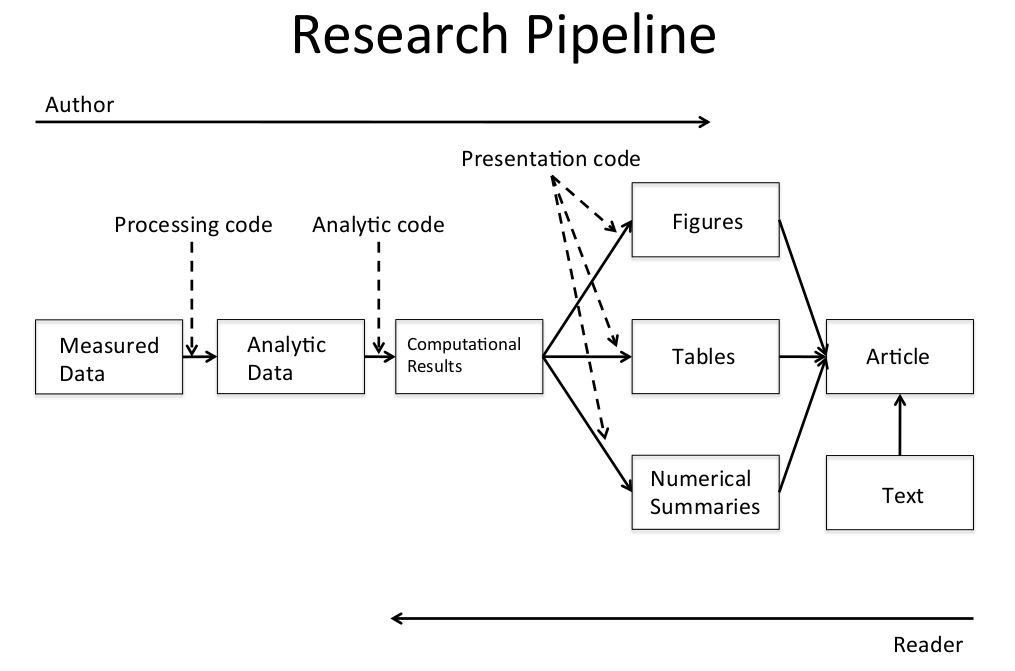
\includegraphics[width=14.1in]{images/researchpipeline}

\hypertarget{ux6570ux636eux5206ux6790ux6b65ux9aa4}{%
\section{数据分析步骤}\label{ux6570ux636eux5206ux6790ux6b65ux9aa4}}

\begin{itemize}
\item
  定义问题

  \begin{itemize}
  \tightlist
  \item
    背后要有科学假设或问题
  \item
    从大到小 具体定义
  \end{itemize}
\item
  定义理想数据

  \begin{itemize}
  \tightlist
  \item
    描述性的 \textless{}- 总体数据
  \item
    探索性的 \textless{}- 有属性测量的样本数据
  \item
    推断性的 \textless{}- 合适的总体 随机采样
  \item
    预测性的 \textless{}- 来自同一总体 有训练集与测试集的样本
  \item
    因果性的 \textless{}- 随机性研究
  \item
    机械性的 \textless{}- 系统中所有组成部分的数据
  \end{itemize}
\item
  决定可获取数据

  \begin{itemize}
  \tightlist
  \item
    网络免费数据
  \item
    购买数据
  \item
    注意使用条款
  \item
    数据不存在 自己创造 \textless{}- 实验
  \end{itemize}
\item
  获取数据

  \begin{itemize}
  \tightlist
  \item
    原始数据
  \item
    引用来源
  \item
    网络数据注明数据来源URL与获取时间
  \end{itemize}
\item
  整理数据

  \begin{itemize}
  \tightlist
  \item
    原始数据需要整理
  \item
    如果事先处理过要搞清楚如何处理的
  \item
    了解数据来源
  \item
    需要重新格式化 采样 \textless{}- 记录步骤
  \item
    判断数据是否合适 不合适重新获取
  \end{itemize}
\item
  探索性数据分析

  \begin{itemize}
  \tightlist
  \item
    描述性总结数据
  \item
    检查缺失值
  \item
    绘制探索性图
  \item
    尝试探索性分析 例如聚类
  \end{itemize}
\item
  统计预测/建模

  \begin{itemize}
  \tightlist
  \item
    基于探索性分析
  \item
    根据问题确定方法
  \item
    数据转换要解释
  \item
    测定的不确定性要考虑
  \end{itemize}
\item
  解释结果

  \begin{itemize}
  \tightlist
  \item
    描述
  \item
    相关
  \item
    推断
  \item
    预测
  \end{itemize}
\item
  质疑结果

  \begin{itemize}
  \tightlist
  \item
    问题
  \item
    数据源
  \item
    处理过程
  \item
    分析
  \item
    结论
  \end{itemize}
\item
  整合写出结果

  \begin{itemize}
  \tightlist
  \item
    从问题角度出发
  \item
    形成一个故事
  \item
    不要包含分析过程除非用来说明问题 消除质疑
  \item
    以故事而不是时间顺序描述
  \item
    图片要漂亮
  \end{itemize}
\item
  写出可重复的R代码

  \begin{itemize}
  \tightlist
  \item
    Rmarkdown文件
  \end{itemize}
\end{itemize}

\hypertarget{ux6570ux636eux5206ux6790ux6587ux4ef6ux7ed3ux6784}{%
\section{数据分析文件结构}\label{ux6570ux636eux5206ux6790ux6587ux4ef6ux7ed3ux6784}}

\begin{itemize}
\item
  Data

  \begin{itemize}
  \tightlist
  \item
    Raw data 来自网络在Readme里注明url 描述 日期
  \item
    Processed data 命名体现处理过程 Readme里注明处理过程
  \end{itemize}
\item
  Figures

  \begin{itemize}
  \tightlist
  \item
    Exploratory figures 不必考虑装饰
  \item
    Final figures 只考虑装饰
  \end{itemize}
\item
  R code

  \begin{itemize}
  \tightlist
  \item
    Raw scripts 不必过分注释 版本控制 不一定用得上
  \item
    Final scripts 注释清晰 包括处理细节 只包括文章需要费分析
  \item
    R Markdown files (optional)
  \end{itemize}
\item
  Text

  \begin{itemize}
  \tightlist
  \item
    Readme files 按步骤记录清晰
  \item
    Text of analysis 包括前言 方法 结果 结论 讲故事 有引用
  \end{itemize}
\end{itemize}

\hypertarget{ux6587ux672cux5316ux7edfux8ba1ux7f16ux7a0b-knitr}{%
\section{文本化统计编程-Knitr}\label{ux6587ux672cux5316ux7edfux8ba1ux7f16ux7a0b-knitr}}

\begin{itemize}
\tightlist
\item
  markdown是轻量化结构语言
\item
  R markdown 是轻量化统计结构语言
\item
  文本+代码块 逻辑清晰
\item
  文本语言可用latex markdown
\item
  代码块可用R
\item
  不用保存输出
\item
  可缓存结果 cacher包
\end{itemize}

\hypertarget{ux7ed3ux679cux901aux8baf}{%
\section{结果通讯}\label{ux7ed3ux679cux901aux8baf}}

\begin{itemize}
\item
  研究论文的信息层级

  \begin{itemize}
  \tightlist
  \item
    题目/作者名单
  \item
    摘要
  \item
    主体/结果
  \item
    支持材料/细节
  \item
    代码/数据
  \end{itemize}
\item
  邮件汇报的信息层级

  \begin{itemize}
  \tightlist
  \item
    题目最好一行一句
  \item
    描述问题 如何实验 总结发现
  \item
    简明扼要
  \item
    如果有问题 写成yes/no形式
  \item
    附件齐全严谨
  \end{itemize}
\end{itemize}

\hypertarget{ux68c0ux67e5ux5217ux8868}{%
\section{检查列表}\label{ux68c0ux67e5ux5217ux8868}}

\begin{itemize}
\tightlist
\item
  数据选取得当
\item
  问题简单专一
\item
  队友靠谱
\item
  兴趣驱动
\item
  不要手动处理数据 全部交给计算机
\item
  少用交互界面 用命令行界面并记录历史
\item
  使用版本控制 处理降速而冷静
\item
  记录软件操作环境 \texttt{sessionInfo()}
\item
  不保存结果保证数据可重复
\item
  使用随机数要说明种子
\item
  原始数据-处理数据-分析-报告
\item
  考虑从哪一步开始数据重复性变差
\end{itemize}

\hypertarget{ux57faux4e8eux8bc1ux636eux7684ux6570ux636eux5206ux6790}{%
\section{基于证据的数据分析}\label{ux57faux4e8eux8bc1ux636eux7684ux6570ux636eux5206ux6790}}

\begin{itemize}
\tightlist
\item
  可重复性研究不保证结果是对的
\item
  发表后研究存在动因 应关注数据生成前的过程
\item
  设定基于证据研究的路线图
\item
  减少研究人员的自由度
\item
  提出区域研究范式
\end{itemize}

\hypertarget{ux7ed3ux679cux53efux89e3ux91ca}{%
\section{结果可解释}\label{ux7ed3ux679cux53efux89e3ux91ca}}

\begin{itemize}
\tightlist
\item
  \href{https://github.com/jsugarelli/xplain}{结果可解释模型}
\end{itemize}

\hypertarget{ux6570ux636eux5206ux6790ux7684ux7406ux8bba}{%
\section{数据分析的理论}\label{ux6570ux636eux5206ux6790ux7684ux7406ux8bba}}

\begin{itemize}
\tightlist
\item
  \href{https://simplystatistics.org/2018/12/11/the-role-of-theory-in-data-analysis/}{数据分析的核心应该是可重复性}
\end{itemize}

\hypertarget{exp}{%
\chapter{探索性数据分析}\label{exp}}

\hypertarget{aces-ux6a21ux578b}{%
\section{ACES 模型}\label{aces-ux6a21ux578b}}

\begin{longtable}[]{@{}lll@{}}
\toprule
\begin{minipage}[b]{0.26\columnwidth}\raggedright
Letter\strut
\end{minipage} & \begin{minipage}[b]{0.17\columnwidth}\raggedright
Step\strut
\end{minipage} & \begin{minipage}[b]{0.48\columnwidth}\raggedright
Notes\strut
\end{minipage}\tabularnewline
\midrule
\endhead
\begin{minipage}[t]{0.26\columnwidth}\raggedright
A\strut
\end{minipage} & \begin{minipage}[t]{0.17\columnwidth}\raggedright
Acquire the data and Assemble the data frame\strut
\end{minipage} & \begin{minipage}[t]{0.48\columnwidth}\raggedright
Find data and import\strut
\end{minipage}\tabularnewline
\begin{minipage}[t]{0.26\columnwidth}\raggedright
C\strut
\end{minipage} & \begin{minipage}[t]{0.17\columnwidth}\raggedright
Clean the data frame\strut
\end{minipage} & \begin{minipage}[t]{0.48\columnwidth}\raggedright
Identify and limit columns, rows, indices, dates, etc.\strut
\end{minipage}\tabularnewline
\begin{minipage}[t]{0.26\columnwidth}\raggedright
E\strut
\end{minipage} & \begin{minipage}[t]{0.17\columnwidth}\raggedright
Explore global properties\strut
\end{minipage} & \begin{minipage}[t]{0.48\columnwidth}\raggedright
Visualize! Basic plots and stats appropriate to the data set\strut
\end{minipage}\tabularnewline
\begin{minipage}[t]{0.26\columnwidth}\raggedright
S\strut
\end{minipage} & \begin{minipage}[t]{0.17\columnwidth}\raggedright
Subset comparisons\strut
\end{minipage} & \begin{minipage}[t]{0.48\columnwidth}\raggedright
Look at (visualize!) initial emergenet variable relationships and subsets\strut
\end{minipage}\tabularnewline
\bottomrule
\end{longtable}

\hypertarget{ux63a2ux7d22ux7ed8ux56feux539fux5219}{%
\section{探索绘图原则}\label{ux63a2ux7d22ux7ed8ux56feux539fux5219}}

\begin{itemize}
\tightlist
\item
  表示可比的对比
\item
  表示因果 解释 机制 系统结构
\item
  表示多元变量(超过2)
\item
  证据整合 目的驱动非工具驱动
\item
  证据描述要标注限定恰当
\item
  内容为王
\end{itemize}

\hypertarget{ux63a2ux7d22ux6027ux7ed8ux56fe}{%
\section{探索性绘图}\label{ux63a2ux7d22ux6027ux7ed8ux56fe}}

\begin{itemize}
\tightlist
\item
  个人理解用
\item
  不用过分关注细节
\item
  基于问题或假设出发
\end{itemize}

\hypertarget{ux5206ux5c42ux805aux7c7b}{%
\section{分层聚类}\label{ux5206ux5c42ux805aux7c7b}}

\begin{itemize}
\tightlist
\item
  找到最近的 聚到一起 找下个最近的
\item
  给出距离范围与距离计算方法

  \begin{itemize}
  \tightlist
  \item
    欧氏距离 多维空间点距 开平方
  \item
    manhattan距离 出租车距离 绝对值
  \end{itemize}
\item
  给出变量间或样本间的关系
\item
  图形可能不稳定 多少样本多少类
\item
  结果是确定的
\item
  选定cut点并不明显
\item
  应该首先用来探索
\end{itemize}

\hypertarget{k-meansux805aux7c7b}{%
\section{k-means聚类}\label{k-meansux805aux7c7b}}

\begin{itemize}
\tightlist
\item
  固定聚类数 给出聚类中心 寻找最近的点 循环
\item
  需要聚类数与聚类距离范围
\item
  需要大量聚类 通过眼睛 交叉检验
\item
  k的经验数值\(\sqrt{n/2}\) 或者根据解释的变量变化多少来选取
\item
  结果不确定 根据聚类数与迭代次数而变化
\end{itemize}

\hypertarget{ux7ef4ux5ea6ux8fd8ux539f}{%
\section{维度还原}\label{ux7ef4ux5ea6ux8fd8ux539f}}

\begin{itemize}
\tightlist
\item
  找到最不相关的数来解释整体方差(统计)在这些数中选取个数最少的来解释原始数据(压缩)
\item
  不一定是真实向量的叠加
\item
  SVD是PCA的一种解法 UDV三个向量 其中U表示行变化模式 D表示方差 V表示列变换模式 这样有助于解释主成分变化
\item
  标准化与否影响结果
\item
  计算量大
\item
  类似探索分析还有因子分析 独立成分分析 潜在语义分析
\item
  impute包可补充缺失值
\item
  t-sne
\end{itemize}

\hypertarget{ux53efux89c6ux5316ux56feux5f62}{%
\section{可视化图形}\label{ux53efux89c6ux5316ux56feux5f62}}

\begin{itemize}
\tightlist
\item
  \href{https://github.com/thomasp85/tweenr}{动态可视化}
\item
  \href{https://github.com/jokergoo/circlize}{弦图}
\item
  \href{https://github.com/hafen/geofacet}{示意地图}
\item
  \href{https://github.com/sjewo/cartogram}{变形地图绘制}
\item
  \href{https://flowingdata.com/2018/07/09/how-to-visualize-recurring-patterns/}{重复模式可视化}
\item
  \href{https://flowingdata.com/2018/01/08/visualizing-the-uncertainty-in-data/}{不确定性可视化}
\item
  周期性作图需要画两个周期来观察其变化 相关
\item
  \href{https://www.nature.com/articles/nbt.1567}{生物数据可视化}
\end{itemize}

\hypertarget{infer}{%
\chapter{统计推断}\label{infer}}

\hypertarget{ux5bfcux8bba}{%
\section{导论}\label{ux5bfcux8bba}}

\begin{itemize}
\tightlist
\item
  定义 用需要考虑不确定度的含噪音的统计学数据推断事实
\item
  工具 随机化 随机采样 采样模型 假设检验 置信区间 概率模型 实验设计 bootstraping 排列交换随机
\item
  类型

  \begin{itemize}
  \tightlist
  \item
    频率派 使用概率的频率解释来控制错误率
  \item
    贝叶斯派 给定概率与数据概率哪个靠谱
  \end{itemize}
\end{itemize}

\hypertarget{ux6982ux7387}{%
\section{概率}\label{ux6982ux7387}}

\begin{itemize}
\tightlist
\item
  术语

  \begin{itemize}
  \tightlist
  \item
    样本空间 Ω
  \item
    事件 样本空间子集 E
  \item
    单独事件 ω
  \item
    空事件 ∅
  \item
    \(ω∈E\) ω发生E发生
  \item
    \(ω∉E\) ω发生E不发生
  \item
    \(E⊂F\) E发生则F发生
  \item
    \(E∩F\) EF一起发生
  \item
    \(E∪F\) EF中至少一个发生
  \item
    \(E∩F=∅\) EF互斥
  \item
    \(E^c\) 或 \(\bar E\) E不发生
  \end{itemize}
\item
  概率

  \begin{enumerate}
  \def\labelenumi{\arabic{enumi}.}
  \tightlist
  \item
    对事件 \(E\subset \Omega\), \(0 \leq P(E) \leq 1\)
  \item
    \(P(\Omega) = 1\)
  \item
    如果 \(E_1\) 与 \(E_2\) 互斥 有\(P(E_1 \cup E_2) = P(E_1) + P(E_2)\).
  \item
    概率无限可加性 \(P(\cup_{i=1}^n A_i) = \sum_{i=1}^n P(A_i)\)
  \item
    \(P(\emptyset) = 0\)
  \item
    \(P(E) = 1 - P(E^c)\)
  \item
    \(P(A \cup B) = P(A) + P(B) - P(A \cap B)\)
  \item
    如果 \(A \subset B\) 则 \(P(A) \leq P(B)\)
  \item
    \(P\left(A \cup B\right) = 1 - P(A^c \cap B^c)\)
  \item
    \(P(A \cap B^c) = P(A) - P(A \cap B)\)
  \item
    \(P(\cup_{i=1}^n E_i) \leq \sum_{i=1}^n P(E_i)\)
  \item
    \(P(\cup_{i=1}^n E_i) \geq \max_i P(E_i)\)
  \end{enumerate}
\item
  随机变量

  \begin{itemize}
  \tightlist
  \item
    实验的数值输出
  \item
    离散随机变量取可数的概率 \(P(X = k)\)
  \item
    连续随机变量取连续区间子集概率 \(P(X \in A)\)
  \end{itemize}
\item
  概率质量函数(PMF)\textless{}- 离散随机变量

  \begin{enumerate}
  \def\labelenumi{\arabic{enumi}.}
  \tightlist
  \item
    对于所有 \(x\) \(p(x) \geq 0\)
  \item
    \(\sum_{x} p(x) = 1\)
  \end{enumerate}
\item
  概率密度函数(PDF)\textless{}- 连续随机变量

  \begin{enumerate}
  \def\labelenumi{\arabic{enumi}.}
  \tightlist
  \item
    对于所有 \(x\) \(f(x) \geq 0\)
  \item
    \(f(x)\) 下面积为1
  \end{enumerate}
\item
  累计概率函数(CDF)

  \begin{itemize}
  \tightlist
  \item
    定义 \(F(x) = P(X \leq x)\)
  \item
    生存函数 \(S(x) = P(X > x)\) \(S(x) = 1 - F(x)\)
  \item
    对于连续函数 CDF是PDF的积分
  \end{itemize}
\item
  分位数 \(\alpha^{th}\)

  \begin{itemize}
  \tightlist
  \item
    \(F(x_\alpha) = \alpha\)
  \item
    \(50^{th}\) 分位数是中位数
  \end{itemize}
\end{itemize}

\hypertarget{ux671fux671b}{%
\section{期望}\label{ux671fux671b}}

\begin{itemize}
\item
  离散随机变量均值 \(E[X] = \sum_x xp(x)\)
\item
  \(E[X]\) 代表质量与位置的中心 \(\{x, p(x)\}\)
\item
  连续随机变量均值 \(E[X] = \mbox{the area under the function}~~~ t f(t)\)
\item
  期望值是线性可加的
\item
  如果 \(a\) 与 \(b\) 不随机 \(X\) 与 \(Y\) 是随机变量

  \begin{itemize}
  \tightlist
  \item
    \(E[aX + b] = a E[X] + b\)
  \item
    \(E[X + Y] = E[X] + E[Y]\)
  \end{itemize}
\item
  样本均值是总体均值\(\mu\)的无偏估计的证明

  \begin{eqnarray*}
    E\left[ \frac{1}{n}\sum_{i=1}^n X_i\right]
    & = & \frac{1}{n} E\left[\sum_{i=1}^n X_i\right] \\
    & = & \frac{1}{n} \sum_{i=1}^n E\left[X_i\right] \\
    & = & \frac{1}{n} \sum_{i=1}^n \mu =  \mu.
  \end{eqnarray*}
\end{itemize}

\hypertarget{ux65b9ux5dee}{%
\section{方差}\label{ux65b9ux5dee}}

\begin{itemize}
\tightlist
\item
  描述随机变量的离散情况
\item
  如果 \(X\) 是均值 \(\mu\) 的随机变量 其方差为\(Var(X) = E[(X - \mu)^2]\)
\item
  离开均值距离期望的平方
\item
  计算公式 \(Var(X) = E[X^2] - E[X]^2\)
\item
  如果 \(a\) 是常数有 \(Var(aX) = a^2 Var(X)\)
\item
  方差的开方是标准差 单位与 \(X\) 一致
\item
  车比雪夫不等式(Chebyshev's inequality)边界极为保守
  \[
  P(|X - \mu| \geq k\sigma) \leq \frac{1}{k^2}
  \]
\end{itemize}

\hypertarget{ux72ecux7acbux6027}{%
\section{独立性}\label{ux72ecux7acbux6027}}

\begin{itemize}
\item
  独立事件

  \begin{itemize}
  \tightlist
  \item
    两事件 \(A\) 与 \(B\) 在 \(P(A \cap B) = P(A)P(B)\) 下独立
  \item
    在 \(P([X \in A] \cap [Y \in B]) = P(X\in A)P(Y\in B)\) 下两随机变量 \(X\) 与 \(Y\) 独立
  \item
    对于一组随机独立变量\(X_1, X_2, \ldots, X_n\)有 \(f(x_1,\ldots, x_n) = \prod_{i=1}^n f_i(x_i)\)
  \item
    iid随机变量(independent and identically distributed) 来自同一分布相互独立的随机变量
  \end{itemize}
\item
  协方差(covariance)

  \begin{itemize}
  \tightlist
  \item
    \(Cov(X, Y) = E[(X - \mu_x)(Y - \mu_y)] = E[X Y] - E[X]E[Y]\)
  \item
    \(Cov(X, Y) = Cov(Y, X)\)
  \item
    \(Cov(X, Y)\) 可以有正负
  \item
    \(|Cov(X, Y)| \leq \sqrt{Var(X) Var(y)}\)
  \end{itemize}
\item
  相关性(correlation)

  \begin{itemize}
  \tightlist
  \item
    \(X\) 与 \(Y\) 的相关性 \(Cor(X, Y) = Cov(X, Y) / \sqrt{Var(X) Var(y)}\)
  \item
    \(-1 \leq Cor(X, Y) \leq 1\)
  \item
    只有对常数 \(a\) 与 \(b\)满足 \(X = a + bY\) 时\(Cor(X, Y) = \pm 1\)
  \item
    \(Cor(X, Y)\) 无单位
  \item
    \(Cor(X, Y) = 0\) 时 \(X\) 与 \(Y\) 不相关
  \item
    \(Cor(X,Y)\) 越接近1 \(X\) 与 \(Y\) 越正相关 反之接近-1 负相关
  \item
    \(\{X_i\}_{i=1}^n\) 是一组随机变量 当 \(\{X_i\}\) 不相关时 \(Var\left(\sum_{i=1}^n a_i X_i + b\right) = \sum_{i=1}^n a_i^2 Var(X_i)\)
  \item
    如果一组随机变量\(\{X_i\}\)不相关 方差的和等于和的方差 非标准差
  \end{itemize}
\item
  样本均值方差的推导

  \begin{eqnarray*}
    Var(\bar X) & = & Var \left( \frac{1}{n}\sum_{i=1}^n X_i \right)\\ \\
    & = & \frac{1}{n^2} Var\left(\sum_{i=1}^n X_i \right)\\ \\
    & = & \frac{1}{n^2} \sum_{i=1}^n Var(X_i) \\ \\
    & = & \frac{1}{n^2} \times n\sigma^2 \\ \\
    & = & \frac{\sigma^2}{n}
  \end{eqnarray*}

  \begin{itemize}
  \tightlist
  \item
    当 \(X_i\) 独立且方差为 \(Var(\bar X) = \frac{\sigma^2}{n}\)
  \item
    \(\sigma/\sqrt{n}\) 为样本均值的标准误
  \item
    样本均值的标准误就是样本均值分布的标准差
  \item
    \(\sigma\) 是一次观察分布的标准差
  \item
    样本均值要比一次观察变化小 因此除以\(\sqrt{n}\)
  \end{itemize}
\item
  样本方差

  \begin{itemize}
  \tightlist
  \item
    \(S^2 = \frac{\sum_{i=1}^n (X_i - \bar X)^2}{n-1}\)
  \item
    总体方差 \(\sigma^2\)的估计
  \item
    计算 \(\sum_{i=1}^n (X_i - \bar X)^2 = \sum_{i=1}^n X_i^2 - n \bar X^2\)
  \item
    均值偏差平方的均值
  \item
    样本方差是总体方差的无偏估计
  \end{itemize}

  \begin{eqnarray*}
    E\left[\sum_{i=1}^n (X_i - \bar X)^2\right] & = & \sum_{i=1}^n E\left[X_i^2\right] - n E\left[\bar X^2\right] \\ \\
    & = & \sum_{i=1}^n \left\{Var(X_i) + \mu^2\right\} - n \left\{Var(\bar X) + \mu^2\right\} \\ \\
    & = & \sum_{i=1}^n \left\{\sigma^2 + \mu^2\right\} - n \left\{\sigma^2 / n + \mu^2\right\} \\ \\
    & = & n \sigma^2 + n \mu ^ 2 - \sigma^2 - n \mu^2 \\ \\
    & = & (n - 1) \sigma^2
  \end{eqnarray*}
\item
  澄清

  \begin{itemize}
  \tightlist
  \item
    假定 \(X_i\) 是 iid 均值 \(\mu\) 方差 \(\sigma^2\)
  \item
    \(S^2\) 估计 \(\sigma^2\)
  \item
    \(S^2\) 的计算涉及除 \(n-1\)
  \item
    \(S / \sqrt{n}\) 估计 \(\sigma / \sqrt{n}\) 是均值的标准误
  \end{itemize}
\end{itemize}

\hypertarget{ux6761ux4ef6ux6982ux7387}{%
\section{条件概率}\label{ux6761ux4ef6ux6982ux7387}}

\begin{itemize}
\tightlist
\item
  \(B\) 为一个事件 有 \(P(B) > 0\)
\item
  \(B\) 出现条件下 \(A\) 的条件概率为 \(P(A ~|~ B) = \frac{P(A \cap B)}{P(B)}\)
\item
  如果 \(A\) 与 \(B\) 独立 有 \(P(A ~|~ B) = \frac{P(A) P(B)}{P(B)} = P(A)\)
\end{itemize}

\hypertarget{ux8d1dux53f6ux65afux5b9aux7406}{%
\section{贝叶斯定理}\label{ux8d1dux53f6ux65afux5b9aux7406}}

\[
P(B ~|~ A) = \frac{P(A ~|~ B) P(B)}{P(A ~|~ B) P(B) + P(A ~|~ B^c)P(B^c)}.
\]

\begin{itemize}
\tightlist
\item
  2*2 列联表 - 诊断测试
\end{itemize}

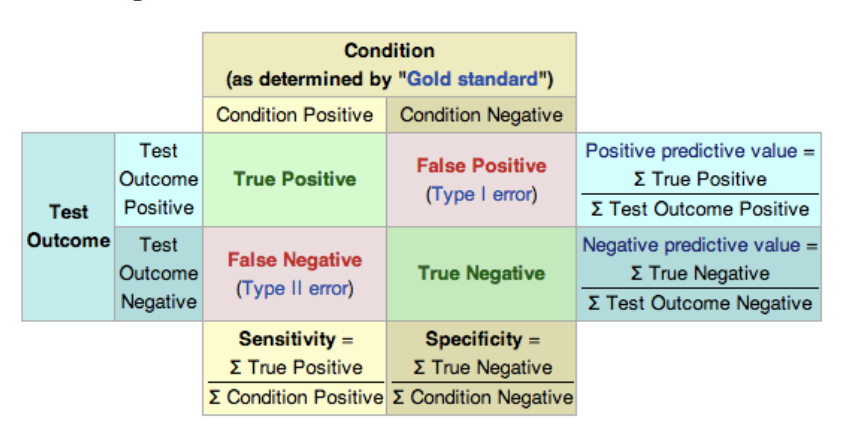
\includegraphics[width=11.74in]{images/error}

\hypertarget{ux5e38ux89c1ux5206ux5e03}{%
\section{常见分布}\label{ux5e38ux89c1ux5206ux5e03}}

\begin{itemize}
\tightlist
\item
  贝努力分布

  \begin{itemize}
  \tightlist
  \item
    二元输出变量
  \item
    数值为0或1 概率\(p\) 与 \(1-p\)
  \item
    \(X\)的PMF是\(P(X = x) = p^x (1 - p)^{1 - x}\)
  \item
    均值 \(p\) 方差 \(p(1 - p)\)
  \item
    如果有iid的贝努力观察\(x_1,\ldots, x_n\) 似然函数 \(\prod_{i=1}^n p^{x_i} (1 - p)^{1 - x_i} = p^{\sum x_i} (1 - p)^{n - \sum x_i}\)
  \item
    似然函数依赖\(x_i\)的和 \(\sum_i x_i / n\) 包含了所有 \(p\) 的可能性
  \item
    最大化似然函数可以得到 \(p\) 的估计
  \end{itemize}
\item
  二项分布

  \begin{itemize}
  \tightlist
  \item
    PMF
    \[
    P(X = x) = 
    \left(
    \begin{array}{c}
    n \\ x
    \end{array}
    \right)
    p^x(1 - p)^{n-x}
    \]
    对于 \(x=0,\ldots,n\)
  \end{itemize}
\item
  正态分布

  \begin{itemize}
  \tightlist
  \item
    PDF \((2\pi \sigma^2)^{-1/2}e^{-(x - \mu)^2/2\sigma^2}\)
  \item
    \(X\) 为均值 \(E[X] = \mu\) 方差 \(Var(X) = \sigma^2\) 的iid随机变量
  \item
    写作\(X\sim \mbox{N}(\mu, \sigma^2)\)
  \item
    均值 \(\mu = 0\) 方差 \(\sigma = 1\) 是标准正态分布
  \item
    标准正态函数写作 \(\phi\)
  \item
    标准正态随机变量用 \(Z\) 表示
  \item
    如果 \(X \sim \mbox{N}(\mu,\sigma^2)\) 并且 \(Z = \frac{X -\mu}{\sigma}\) 是标准正态函数
  \item
    如果 \(Z\) 是标准正态函数 \(X = \mu + \sigma Z \sim \mbox{N}(\mu, \sigma^2)\)
  \item
    非标准正态密度函数 \(\phi\{(x - \mu) / \sigma\}/\sigma\)
  \item
    正态似然函数对方差的估计是有偏的
  \item
    正态的和是正态 样本均值正态
  \item
    正态的平方是卡方
  \item
    \href{http://songshuhui.net/archives/76501}{正态分布}
  \end{itemize}
\item
  泊松分布

  \begin{itemize}
  \tightlist
  \item
    PMF \(P(X = x; \lambda) = \frac{\lambda^x e^{-\lambda}}{x!}\)
  \item
    均值方差均为 \(\lambda\)
  \item
    可看做很短时间间隔中发生事件的概率 模拟速率 其中\(\lambda * h\)小于1 则各时间段独立
  \item
    \(X \sim Poisson(\lambda t)\) \(\lambda = E[X / t]\)是速率 \(t\) 是总时间
  \item
    \(n\) 大 \(p\) 小是对二项分布的模拟
  \item
    \(X \sim \mbox{Binomial}(n, p)\), \(\lambda = n p\)
  \end{itemize}
\end{itemize}

\hypertarget{ux6e10ux8fdb}{%
\section{渐进}\label{ux6e10ux8fdb}}

\begin{itemize}
\tightlist
\item
  样本接近无穷大时统计量的行为
\item
  频率派的基石
\item
  大数理论(LLN) 样本数量越多 均值接近期望
\item
  中心极限理论 (CLT) iid 变量均值的分布标准化后随样本数增加接近标准正态分布
  \[
  \frac{\bar X_n - \mu}{\sigma / \sqrt{n}} = 
    \frac{\mbox{Estimate} - \mbox{Mean of estimate}}{\mbox{Std. Err. of estimate}}
  \]
\item
  可根据变量分布来 知道均值 方差 计算出样本均值标准误 就可以根据CLT计算逼近的统计量
\item
  置信区间

  \begin{itemize}
  \tightlist
  \item
    根据CLT随机区间\(\bar X_n \pm z_{1-\alpha/2}\sigma / \sqrt{n}\) 包括 \(\mu\) 的概率逼近于 100\((1-\alpha)\)\% \(z_{1-\alpha/2}\)为标准正态分布\(1-\alpha/2\)的分位数 \(100(1 - \alpha)\)\% 为置信区间 \(\sigma\) 可用样本估计 \(s\) 来近似
  \item
    估计是基于分布假设的 如果分布有解析解 则置信区间可以更准确的得到估计
  \item
    先生成不依赖参数的统计量
  \item
    根据统计量的概率分布计算参数的边界
  \end{itemize}
\end{itemize}

\hypertarget{ux7f6eux4fe1ux533aux95f4}{%
\section{置信区间}\label{ux7f6eux4fe1ux533aux95f4}}

\begin{itemize}
\tightlist
\item
  卡方分布

  \begin{itemize}
  \tightlist
  \item
    假定 \(S^2\) 是来自\(n\)个 iid \(N(\mu,\sigma^2)\) 数据样本的方差 有\(\frac{(n - 1) S^2}{\sigma^2} \sim \chi^2_{n-1}\) 符合自由度\(n-1\)的卡方分布
  \item
    不对称分布
  \item
    均值是自由度 方差是两倍的自由度
  \item
    方差的置信区间
  \end{itemize}
\end{itemize}

\begin{eqnarray*}
  1 - \alpha & = & P \left( \chi^2_{n-1, \alpha/2} \leq  \frac{(n - 1) S^2}{\sigma^2} \leq  \chi^2_{n-1,1 - \alpha/2} \right) \\ \\
& = &  P\left(\frac{(n-1)S^2}{\chi^2_{n-1,1-\alpha/2}} \leq \sigma^2 \leq 
\frac{(n-1)S^2}{\chi^2_{n-1,\alpha/2}} \right) \\
\end{eqnarray*}

\begin{itemize}
\tightlist
\item
  \(\left[\frac{(n-1)S^2}{\chi^2_{n-1,1-\alpha/2}}, \frac{(n-1)S^2}{\chi^2_{n-1,\alpha/2}}\right]\) 是 \(\sigma^2\) 的 \(100(1-\alpha)\%\) 置信区间
\item
  依赖正态性假设 开方后得到 \(\sigma\) 的置信区间
\item
  Gosset的 t 分布

  \begin{itemize}
  \tightlist
  \item
    比正态分布尾厚
  \item
    考虑自由度 自由度大时接近正态分布
  \item
    \(\frac{Z}{\sqrt{\frac{\chi^2}{df}}}\)
  \item
    假定 \((X_1,\ldots,X_n)\) 是 iid \(N(\mu,\sigma^2)\) 有 \(\frac{\bar X - \mu}{\sigma / \sqrt{n}}\) 是标准正态分布 \(\sqrt{\frac{(n - 1) S^2}{\sigma^2 (n - 1)}} = S / \sigma\) 是卡方除以自由度的开方
  \item
    有
    \[
    \frac{\frac{\bar X - \mu}{\sigma /\sqrt{n}}}{S/\sigma}  
    = \frac{\bar X - \mu}{S/\sqrt{n}}
    \]
    服从自由度\(n-1\)的\(t\)分布
  \item
    均值的置信区间
  \end{itemize}

  \begin{eqnarray*}
  &   & 1 - \alpha \\
  & = & P\left(-t_{n-1,1-\alpha/2} \leq \frac{\bar X - \mu}{S/\sqrt{n}} \leq t_{n-1,1-\alpha/2}\right) \\ \\
  & = & P\left(\bar X - t_{n-1,1-\alpha/2} S / \sqrt{n} \leq \mu  
      \leq \bar X + t_{n-1,1-\alpha/2}S /\sqrt{n}\right)
  \end{eqnarray*}

  \(t_{df,\alpha}\) 是t分布的 \(\alpha^{th}\) 分位数 自由度 \(df\)

  \begin{itemize}
  \tightlist
  \item
    t检验不适合有偏分布 置信区间中心也不在均值上
  \end{itemize}
\end{itemize}

\hypertarget{ux4f3cux7136ux51fdux6570}{%
\section{似然函数}\label{ux4f3cux7136ux51fdux6570}}

\begin{itemize}
\tightlist
\item
  一组数据的似然函数是数据固定下参数的联合概率密度函数
\item
  似然函数可用来估计参数 是参数的函数
\item
  似然函数比估计两个可能参数值的可能性
\item
  给定模型与数据 似然函数包含所有参数可能性
\item
  样本独立时 参数的似然函数是各独立样本似然函数的乘积
\item
  参数使似然函数概率取最大值时真实的可能性更大 更支持这组数据 这个估计是最大似然估计(MLE)
\end{itemize}

\hypertarget{ux8d1dux53f6ux65afux63a8ux65ad}{%
\section{贝叶斯推断}\label{ux8d1dux53f6ux65afux63a8ux65ad}}

\begin{itemize}
\tightlist
\item
  \(\mbox{Posterior} \propto \mbox{Likelihood} \times \mbox{Prior}\)
\item
  先验beta分布

  \begin{itemize}
  \tightlist
  \item
    01之间
  \item
    依赖 \(\alpha\) \(\beta\) 的概率密度函数
  \end{itemize}
\end{itemize}

\[
\frac{\Gamma(\alpha +  \beta)}{\Gamma(\alpha)\Gamma(\beta)}
 p ^ {\alpha - 1} (1 - p) ^ {\beta - 1} ~~~~\mbox{for} ~~ 0 \leq p \leq 1
\]

\begin{itemize}
\tightlist
\item
  均值 \(\alpha / (\alpha + \beta)\)
\item
  方差 \(\frac{\alpha \beta}{(\alpha + \beta)^2 (\alpha + \beta + 1)}\)
\item
  \(\alpha = \beta = 1\) 为均匀分布
\item
  后验beta分布

  \begin{itemize}
  \tightlist
  \item
    参数\(\tilde \alpha = x + \alpha\) \(\tilde \beta = n - x + \beta\) 的beta分布
  \end{itemize}
\end{itemize}

\begin{align}
\mbox{Posterior} &\propto  p^x(1 - p)^{n-x} \times p^{\alpha -1} (1 - p)^{\beta - 1} \\
                 &  =      p^{x + \alpha - 1} (1 - p)^{n - x + \beta - 1}
\end{align}

\begin{itemize}
\tightlist
\item
  后验均值
\end{itemize}

\begin{align}
E[p ~|~ X] & =   \frac{\tilde \alpha}{\tilde \alpha + \tilde \beta}\\ \\
& =  \frac{x + \alpha}{x + \alpha + n - x + \beta}\\ \\
& =  \frac{x + \alpha}{n + \alpha + \beta} \\ \\
& =  \frac{x}{n} \times \frac{n}{n + \alpha + \beta} + \frac{\alpha}{\alpha + \beta} \times \frac{\alpha + \beta}{n + \alpha + \beta} \\ \\
& =  \mbox{MLE} \times \pi + \mbox{Prior Mean} \times (1 - \pi)
\end{align}

\begin{itemize}
\tightlist
\item
  后验均值是先验均值与最大似然估计的混合
\item
  当 \(n\) 变大 \(\pi\) 接近 \(1\) 先验作用小
\item
  当 \(n\) 很小 先验作用大
\item
  当数据量够大时 先验概率作用就很小了
\item
  当先验概率足够稳定 数据就作用不大了
\item
  信任区间

  \begin{itemize}
  \tightlist
  \item
    \(95\%\) 信任区间 \([a, b]\) 会满足\(P(p \in [a, b] ~|~ x) = .95\)
  \item
    最高后验密度 (HPD) 区间
  \end{itemize}
\end{itemize}

\hypertarget{ux4e24ux72ecux7acbux6837ux672ctux68c0ux9a8c}{%
\section{两独立样本t检验}\label{ux4e24ux72ecux7acbux6837ux672ctux68c0ux9a8c}}

\begin{itemize}
\item
  \(X_1,\ldots,X_{n_x}\) 为 iid \(N(\mu_x,\sigma^2)\)
\item
  \(Y_1,\ldots,Y_{n_y}\) 为 iid \(N(\mu_y, \sigma^2)\)
\item
  \(\bar X\), \(\bar Y\), \(S_x\), \(S_y\) 为均值与标准差
\item
  根据均值与方差的线性组合 有 \(\bar Y - \bar X\) 也是正态 均值 \(\mu_y - \mu_x\) 方差 \(\sigma^2 (\frac{1}{n_x} + \frac{1}{n_y})\)
\item
  混合方差为 \(S_p^2 = \{(n_x - 1) S_x^2 + (n_y - 1) S_y^2\}/(n_x + n_y - 2)\) 为\(\sigma^2\)的良好估计
\item
  该估计为无偏估计

  \begin{eqnarray*}
    E[S_p^2] & = & \frac{(n_x - 1) E[S_x^2] + (n_y - 1) E[S_y^2]}{n_x + n_y - 2}\\
            & = & \frac{(n_x - 1)\sigma^2 + (n_y - 1)\sigma^2}{n_x + n_y - 2}
    \end{eqnarray*}
\item
  该估计独立于 \(\bar Y - \bar X\) 因为方差独立于均值
\item
  两个独立的卡方变量之和是自由度之和的卡方值

  \begin{eqnarray*}
      (n_x + n_y - 2) S_p^2 / \sigma^2 & = & (n_x - 1)S_x^2 /\sigma^2 + (n_y - 1)S_y^2/\sigma^2 \\ \\
      & = & \chi^2_{n_x - 1} + \chi^2_{n_y-1} \\ \\
      & = & \chi^2_{n_x + n_y - 2}
    \end{eqnarray*}
\item
  构建统计量
  \[
    \frac{\frac{\bar Y - \bar X - (\mu_y - \mu_x)}{\sigma \left(\frac{1}{n_x} + \frac{1}{n_y}\right)^{1/2}}}{\sqrt{\frac{(n_x + n_y - 2) S_p^2}{(n_x + n_y - 2)\sigma^2}}}
    = \frac{\bar Y - \bar X - (\mu_y - \mu_x)}{S_p \left(\frac{1}{n_x} + \frac{1}{n_y}\right)^{1/2}}
  \]
\item
  该统计量为符合自由度 \(n_x + n_y - 2\) 的 \(t\) 分布
\item
  置信区间
  \[
    \bar Y - \bar X \pm t_{n_x + n_y - 2, 1 - \alpha/2}S_p\left(\frac{1}{n_x} + \frac{1}{n_y}\right)^{1/2}
  \]
\item
  方差不等
  \[
    \bar Y - \bar X \sim N\left(\mu_y - \mu_x, \frac{s_x^2}{n_x} + \frac{s_y^2}{n_y}\right)
  \]
\item
  统计量
  \[
    \frac{\bar Y - \bar X - (\mu_y - \mu_x)}{\left(\frac{s_x^2}{n_x} + \frac{s_y^2}{n_y}\right)^{1/2}}
  \]
  近似于自由度
  \[
    \frac{\left(S_x^2 / n_x + S_y^2/n_y\right)^2}
    {\left(\frac{S_x^2}{n_x}\right)^2 / (n_x - 1) +
      \left(\frac{S_y^2}{n_y}\right)^2 / (n_y - 1)}
  \]
  的\(t\)分布
\end{itemize}

\hypertarget{ux5047ux8bbeux68c0ux9a8c}{%
\section{假设检验}\label{ux5047ux8bbeux68c0ux9a8c}}

\begin{itemize}
\tightlist
\item
  使用数据做决定
\item
  空假设 \(H_0\) 无变化
\item
  备择假设 \(H_a\) 或大 或小 或不等
\item
  真值表
\end{itemize}

\begin{longtable}[]{@{}lll@{}}
\toprule
Truth & Decide & Result\tabularnewline
\midrule
\endhead
\(H_0\) & \(H_0\) & Correctly accept null\tabularnewline
\(H_0\) & \(H_a\) & Type I error\tabularnewline
\(H_a\) & \(H_a\) & Correctly reject null\tabularnewline
\(H_a\) & \(H_0\) & Type II error\tabularnewline
\bottomrule
\end{longtable}

\begin{itemize}
\tightlist
\item
  Z检验

  \begin{itemize}
  \tightlist
  \item
    Z检验 \(H_0:\mu = \mu_0\) 与

    \begin{itemize}
    \tightlist
    \item
      \(H_1: \mu < \mu_0\)
    \item
      \(H_2: \mu \neq \mu_0\)
    \item
      \(H_3: \mu > \mu_0\)
    \end{itemize}
  \item
    检验统计量 \(TS = \frac{\bar{X} - \mu_0}{S / \sqrt{n}}\)
  \item
    拒绝空假设条件

    \begin{itemize}
    \tightlist
    \item
      \(TS \leq -Z_{1 - \alpha}\)
    \item
      \(|TS| \geq Z_{1 - \alpha / 2}\)
    \item
      \(TS \geq Z_{1 - \alpha}\)
    \end{itemize}
  \item
    样本数要足够 否则选 \(t\) 检验
  \item
    通过 \(\alpha\) 控制了 Type I error 但没控制 \(\beta\) Type II error 所以结论为没有拒绝 \(H_0\) 而不是接受 \(H_0\)
  \item
    拒绝 \(H_0\) 的值域为拒绝域
  \end{itemize}
\item
  二项分布不易做正态假设可精确计算拒绝域
\end{itemize}

\hypertarget{pux503c}{%
\section{P值}\label{pux503c}}

\begin{itemize}
\tightlist
\item
  假定没有事发生 出现状况的可能性
\item
  先定义分布 然后计算相关统计量 对比常见阈值看数值是否够极端
\item
  阈值为达到显著性水平 与p值有区别
\item
  p值可设定任意显著性水平 小于就可以拒绝
\item
  两尾检验 单尾概率翻倍
\item
  独立于假设检验 但常常一起使用
\end{itemize}

\hypertarget{ux529fux6548}{%
\section{功效}\label{ux529fux6548}}

\begin{itemize}
\tightlist
\item
  错误拒绝空假设的概率为功效(power)
\item
  Power \(= 1 - \beta\) 对 Type II error 的控制
\item
  正态分布假设下的推导
\end{itemize}

\begin{align}
1 -\beta & = 
P\left(\frac{\bar X - 30}{\sigma /\sqrt{n}} > z_{1-\alpha} ~|~ \mu = \mu_a \right)\\
& = P\left(\frac{\bar X - \mu_a + \mu_a - 30}{\sigma /\sqrt{n}} > z_{1-\alpha} ~|~ \mu = \mu_a \right)\\ \\
& = P\left(\frac{\bar X - \mu_a}{\sigma /\sqrt{n}} > z_{1-\alpha} - \frac{\mu_a - 30}{\sigma /\sqrt{n}} ~|~ \mu = \mu_a \right)\\ \\
& = P\left(Z > z_{1-\alpha} - \frac{\mu_a - 30}{\sigma /\sqrt{n}} ~|~ \mu = \mu_a \right)\\ \\
\end{align}

\begin{Shaded}
\begin{Highlighting}[]
\NormalTok{sigma <-}\StringTok{ }\DecValTok{10}\NormalTok{; mu_}\DecValTok{0}\NormalTok{ =}\StringTok{ }\DecValTok{0}\NormalTok{; mu_a =}\StringTok{ }\DecValTok{2}\NormalTok{; n <-}\StringTok{ }\DecValTok{100}\NormalTok{; alpha =}\StringTok{ }\FloatTok{.05}
\KeywordTok{plot}\NormalTok{(}\KeywordTok{c}\NormalTok{(}\OperatorTok{-}\DecValTok{3}\NormalTok{, }\DecValTok{6}\NormalTok{),}\KeywordTok{c}\NormalTok{(}\DecValTok{0}\NormalTok{, }\KeywordTok{dnorm}\NormalTok{(}\DecValTok{0}\NormalTok{)), }\DataTypeTok{type =} \StringTok{"n"}\NormalTok{, }\DataTypeTok{frame =}\NormalTok{ F, }\DataTypeTok{xlab =} \StringTok{"Z value"}\NormalTok{, }\DataTypeTok{ylab =} \StringTok{""}\NormalTok{)}
\NormalTok{xvals <-}\StringTok{ }\KeywordTok{seq}\NormalTok{(}\OperatorTok{-}\DecValTok{3}\NormalTok{, }\DecValTok{6}\NormalTok{, }\DataTypeTok{length =} \DecValTok{1000}\NormalTok{)}
\KeywordTok{lines}\NormalTok{(xvals, }\KeywordTok{dnorm}\NormalTok{(xvals), }\DataTypeTok{type =} \StringTok{"l"}\NormalTok{, }\DataTypeTok{lwd =} \DecValTok{3}\NormalTok{)}
\KeywordTok{lines}\NormalTok{(xvals, }\KeywordTok{dnorm}\NormalTok{(xvals, }\DataTypeTok{mean =} \KeywordTok{sqrt}\NormalTok{(n) }\OperatorTok{*}\StringTok{ }\NormalTok{(mu_a }\OperatorTok{-}\StringTok{ }\NormalTok{mu_}\DecValTok{0}\NormalTok{) }\OperatorTok{/}\StringTok{ }\NormalTok{sigma), }\DataTypeTok{lwd =}\DecValTok{3}\NormalTok{)}
\KeywordTok{abline}\NormalTok{(}\DataTypeTok{v =} \KeywordTok{qnorm}\NormalTok{(}\DecValTok{1} \OperatorTok{-}\StringTok{ }\NormalTok{alpha))}
\end{Highlighting}
\end{Shaded}

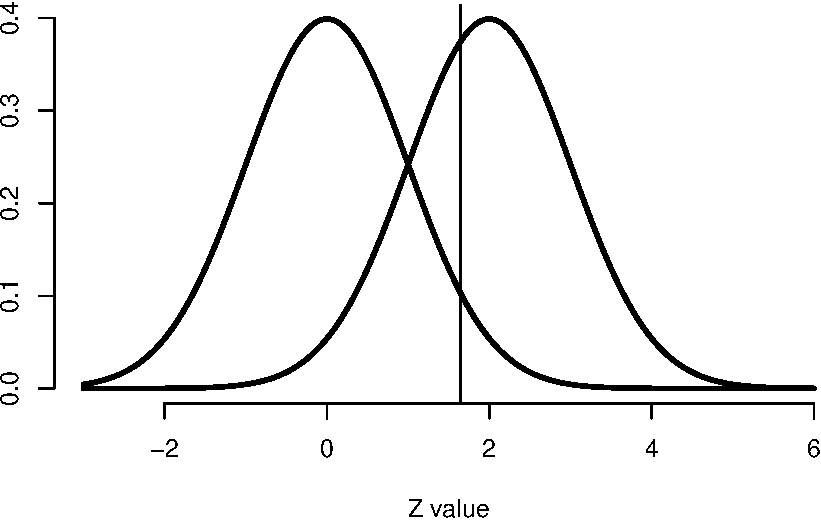
\includegraphics{datadown_files/figure-latex/power-1.pdf}
- 计算步骤
- 考虑 \(H_0 : \mu = \mu_0\) 与 \(H_a : \mu > \mu_0\) 且在\(H_a\)下 \(\mu = \mu_a\)
- 在 \(H_0\) 下统计量 \(Z = \frac{\sqrt{n}(\bar X - \mu_0)}{\sigma}\) 符合 \(N(0, 1)\)
- 在\(H_a\)下 \(Z\) 是 \(N\left( \frac{\sqrt{n}(\mu_a - \mu_0)}{\sigma}, 1\right)\)
- 如果 \(Z > Z_{1-\alpha}\) 拒绝空假设 也就是给定条件下功效不够
- 当检验 \(H_a : \mu > \mu_0\), 如果功效为 \(1 - \beta\) 那么
\(1 - \beta = P\left(Z > z_{1-\alpha} - \frac{\mu_a - \mu_0}{\sigma /\sqrt{n}} ~|~ \mu = \mu_a \right) = P(Z > z_{\beta})\) 也就是 \(z_{1-\alpha} - \frac{\sqrt{n}(\mu_a - \mu_0)}{\sigma} = z_{\beta}\)
- \(\mu_a\), \(\sigma\), \(n\), \(\beta\), \(\mu_0\), \(\alpha\) 给定五个可解出剩余的
- 两尾检验考虑 \(\alpha / 2\)
- 功效在 \(\alpha\) 提高 单尾检验功效高于两尾 \(\mu_1\) 距离 \(\mu_0\) 远功效大 样本数提高功效高
- 计算功效不需要特定样本 只需要指定 \(\frac{\mu_a - \mu_0}{\sigma}\) 也就是有效样本大小 无单位
- R 中使用 \texttt{power.t.test} 来计算 \(t\) 检验功效相关参数 指定多数求一个

\hypertarget{ux591aux91cdux6bd4ux8f83}{%
\section{多重比较}\label{ux591aux91cdux6bd4ux8f83}}

\begin{itemize}
\tightlist
\item
  多次进行比较会导致错误率与校正出现问题
\item
  False positive rate 错误结果是显著的比率 \(\alpha\) 样本数增大错误增加
\item
  Family wise error rate (FWER) 所有比较中至少一个假阳性比率

  \begin{itemize}
  \tightlist
  \item
    Bonferroni correction
  \item
    假设你进行m次测试 控制 \(\alpha\) 在某水平 计算所有测试的 \(p\) 值 将 \(\alpha\) 设为 \(\frac{\alpha}{m}\) 所有测试都在这个置信度下进行
  \item
    容易计算 过于保守
  \end{itemize}
\item
  False discovery rate (FDR) 声称显著是错误的概率

  \begin{itemize}
  \tightlist
  \item
    \(m\) 次测试 水平 \(\alpha\) 计算 \(p\) 值
  \item
    排序 \(P_{(i)} \leq \alpha \times \frac{i}{m}\) 为显著
  \item
    相对容易计算 不保守 允许一定的假阳性
  \end{itemize}
\item
  调节p值

  \begin{itemize}
  \tightlist
  \item
    \(P_i^{fwer} = \max{m \times P_i,1}\) 类似FWER处理 \(\alpha\) 的方式处理 \(p\) 按照正常 \(\alpha\) 检测
  \end{itemize}
\item
  一般情况对 \(p\) 值用 bonferroni/BH矫正就够了
\item
  对比间依赖强烈考虑 method=``BY''
\item
  \href{http://yufree.github.io/blogcn/2013/12/16/rgabriel-package.html}{多重比较从原理到应用} 从实用角度分类 适合常见科研实验结果处理
\end{itemize}

\hypertarget{ux91cdux91c7ux6837ux63a8ux65ad}{%
\section{重采样推断}\label{ux91cdux91c7ux6837ux63a8ux65ad}}

\begin{itemize}
\tightlist
\item
  jackknife

  \begin{itemize}
  \tightlist
  \item
    用来无偏估计偏差与标准误
  \item
    每次估计删掉一个数据 \(\bar \theta = \frac{1}{n}\sum_{i=1}^n \hat \theta_{i}\)
  \item
    偏差 \((n - 1) \left(\bar \theta - \hat \theta\right)\)
  \item
    标准误 \(\left[\frac{n-1}{n}\sum_{i=1}^n (\hat \theta_i - \bar\theta )^2\right]^{1/2}\)
  \item
    可用来估计分位数 是bootstrap的线性逼近 但性质不好
  \item
    假观察量角度理解jackknife \(\mbox{Pseudo Obs} = n \hat \theta - (n - 1) \hat \theta_{i}\) 生成原数据集
  \end{itemize}
\item
  bootstrap
\end{itemize}

\hypertarget{ux6982ux5ff5ux53efux89c6ux5316}{%
\section{概念可视化}\label{ux6982ux5ff5ux53efux89c6ux5316}}

\begin{itemize}
\tightlist
\item
  \href{http://rpsychologist.com/d3/correlation/}{统计概念可视化}

  \begin{itemize}
  \tightlist
  \item
    构建置信区间与求标准误
  \item
    假定采样分布是总体分布 重采样估计统计量
  \item
    有放回的重采样 \(B\) 次 \(N\) 个样本 得到估计统计量的一个分布 直接计算置信区间
  \item
    非参方法 偏差小 \href{http://galton.uchicago.edu/~eichler/stat24600/Handouts/bootstrap.pdf}{进阶指南}
  \end{itemize}
\item
  置换检验

  \begin{itemize}
  \tightlist
  \item
    分组对比时取消原分组随机分组
  \item
    重复进行 记录分组差异
  \item
    对比原参数与置换后参数差异进行推断
  \end{itemize}
\end{itemize}

\hypertarget{reg}{%
\chapter{回归模型}\label{reg}}

\hypertarget{ux56deux5f52ux6a21ux578bux5bfcux8bba}{%
\section{回归模型导论}\label{ux56deux5f52ux6a21ux578bux5bfcux8bba}}

\begin{itemize}
\tightlist
\item
  Francis Galton 1885年用父母身高预测子女身高的案例
\item
  考虑单变量的数据代表:最小二乘值

  \begin{itemize}
  \tightlist
  \item
    最小二乘值物理意义为质心
  \item
    最小二乘统计学意义是平均值
  \item
    可用不等式解 也可用求导方法解
  \end{itemize}
\end{itemize}

\begin{align} 
\sum_{i=1}^n (Y_i - \mu)^2 & = \
\sum_{i=1}^n (Y_i - \bar Y + \bar Y - \mu)^2 \\ 
& = \sum_{i=1}^n (Y_i - \bar Y)^2 + \
2 \sum_{i=1}^n (Y_i - \bar Y)  (\bar Y - \mu) +\
\sum_{i=1}^n (\bar Y - \mu)^2 \\
& = \sum_{i=1}^n (Y_i - \bar Y)^2 + \
2 (\bar Y - \mu) \sum_{i=1}^n (Y_i - \bar Y)  +\
\sum_{i=1}^n (\bar Y - \mu)^2 \\
& = \sum_{i=1}^n (Y_i - \bar Y)^2 + \
2 (\bar Y - \mu)  (\sum_{i=1}^n Y_i - n \bar Y) +\
\sum_{i=1}^n (\bar Y - \mu)^2 \\
& = \sum_{i=1}^n (Y_i - \bar Y)^2 + \sum_{i=1}^n (\bar Y - \mu)^2\\ 
& \geq \sum_{i=1}^n (Y_i - \bar Y)^2 \
\end{align}

\begin{itemize}
\tightlist
\item
  通过原点的回归

  \begin{itemize}
  \tightlist
  \item
    最小化\(\sum_{i=1}^n (Y_i - X_i \beta)^2\)
  \item
    两变量关系用回归线解释
  \end{itemize}
\item
  \href{https://www.listendata.com/2018/03/regression-analysis.html}{回归分析种类大全}
\end{itemize}

\hypertarget{ux672fux8bed}{%
\section{术语}\label{ux672fux8bed}}

\begin{itemize}
\tightlist
\item
  \(X_1, X_2, \ldots, X_n\) 表示 \(n\) 个数据点
\item
  \(Y_1, \ldots , Y_n\) 表示另外 \(n\) 个数据点
\item
  用希腊字母表示不知道的东西 如 \(\mu\)
\item
  大写字母表示概念值 小写字母表示真实值 如 \(P(X_i > x)\)
\item
  \(\bar X = \frac{1}{n}\sum_{i=1}^n X_i\) 表示均值 数据的中心趋向
\item
  \(\tilde X_i = X_i - \bar X\) 表示对数据中心化 均值为0
\item
  均值为数据的最小二乘估计
\item
  \(S^2 = \frac{1}{n-1} \sum_{i=1}^n (X_i - \bar X)^2 = \frac{1}{n-1} \left( \sum_{i=1}^n X_i^2 - n \bar X ^ 2 \right)\) 表示方差
\item
  \(S\) 为标准差 数据的离散程度
\item
  \(X_i / s\) 表示数据缩放 方差为1
\item
  \(Z_i = \frac{X_i - \bar X}{s}\) 表示数据的标准化 先中心化再标准化
\item
  \(Cov(X, Y) = \frac{1}{n-1}\sum_{i=1}^n (X_i - \bar X) (Y_i - \bar Y)= \frac{1}{n-1}\left( \sum_{i=1}^n X_i Y_i - n \bar X \bar Y\right)\) 表示协方差
\item
  \(Cor(X, Y) = \frac{Cov(X, Y)}{S_x S_y}\) 表示相关性

  \begin{itemize}
  \tightlist
  \item
    \(Cor(X, Y) = Cor(Y, X)\)
  \item
    \(-1 \leq Cor(X, Y) \leq 1\)
  \item
    \(Cor(X, Y)\) 度量线性关系强度
  \item
    \(Cor(X, Y) = 0\) 表示无线性关系
  \end{itemize}
\end{itemize}

\hypertarget{ux56deux5f52ux7ebfux7684ux6700ux5c0fux4e8cux4e58ux56deux5f52}{%
\section{回归线的最小二乘回归}\label{ux56deux5f52ux7ebfux7684ux6700ux5c0fux4e8cux4e58ux56deux5f52}}

\begin{itemize}
\tightlist
\item
  用最小二乘法寻找回归线 最小化 \(\sum_{i=1}^n \{Y_i - (\beta_0 + \beta_1 X_i)\}^2\)
\item
  如果定义 \(\mu_i = \beta_0\) \(\hat \beta_0 = \bar Y\) 不考虑其他变量 \(Y\) 的均值就是最小二乘估计
\item
  如果定义 \(\mu_i = X_i \beta_1\) \(\hat \beta_1 = \frac{\sum_{i=1^n} Y_i X_i}{\sum_{i=1}^n X_i^2}\) 如果考虑过原点线的回归 斜率如上
\item
  如果考虑 \(\mu_i = \beta_0 + \beta_1 X_i\)
\end{itemize}

\begin{align} \
\sum_{i=1}^n (Y_i - \hat \mu_i) (\hat \mu_i - \mu_i) 
= & \sum_{i=1}^n (Y_i - \hat\beta_0 - \hat\beta_1 X_i) (\hat \beta_0 + \hat \beta_1 X_i - \beta_0 - \beta_1 X_i) \\
= & (\hat \beta_0 - \beta_0) \sum_{i=1}^n (Y_i - \hat\beta_0 - \hat \beta_1 X_i) + (\beta_1 - \beta_1)\sum_{i=1}^n (Y_i - \hat\beta_0 - \hat \beta_1 X_i)X_i\\
\end{align}

\begin{itemize}
\tightlist
\item
  解为\(\hat \beta_1 = Cor(Y, X) \frac{Sd(Y)}{Sd(X)} ~~~ \hat \beta_0 = \bar Y - \hat \beta_1 \bar X\)
\item
  如果标准化数据 \(\{ \frac{X_i - \bar X}{Sd(X)}, \frac{Y_i - \bar Y}{Sd(Y)}\}\) 解为\(Cor(Y, X)\)
\item
  回归是因变量向自己均值回归与向自变量相关回归的平衡
\end{itemize}

\hypertarget{ux7edfux8ba1ux7ebfux6027ux56deux5f52ux6a21ux578b}{%
\section{统计线性回归模型}\label{ux7edfux8ba1ux7ebfux6027ux56deux5f52ux6a21ux578b}}

\begin{itemize}
\tightlist
\item
  最小二乘是一种估计方法,做推断需要模型
\item
  建立线性回归的概率模型\(Y_i = \beta_0 + \beta_1 X_i + \epsilon_{i}\)
\item
  \(\epsilon_{i}\) 为 iid \(N(0, \sigma^2)\)
\item
  \(E[Y_i ~|~ X_i = x_i] = \mu_i = \beta_0 + \beta_1 x_i\)
\item
  \(Var(Y_i ~|~ X_i = x_i) = \sigma^2\)
\item
  对\(N(\mu_i, \sigma^2)\)独立变量 \(Y\) 进行极大似然估计
\item
  \({\cal L}(\beta, \sigma) = \prod_{i=1}^n \left\{(2 \pi \sigma^2)^{-1/2}\exp\left(-\frac{1}{2\sigma^2}(y_i - \mu_i)^2 \right) \right\}\)
\item
  取对数有 \(-2 \log\{ {\cal L}(\beta, \sigma) \} = \frac{1}{\sigma^2} \sum_{i=1}^n (y_i - \mu_i)^2 + n\log(\sigma^2)\)
\item
  最小二乘估计就是极大似然估计
\item
  \(\hat \beta_1 = Cor(Y, X) \frac{Sd(Y)}{Sd(X)} ~~~ \hat \beta_0 = \bar Y - \hat \beta_1 \bar X\)
\item
  截距是自变量为0时 \(Y\) 的期望 斜率是自变量变化一个单位对 \(Y\) 的影响
\end{itemize}

\hypertarget{ux6b8bux5dee}{%
\section{残差}\label{ux6b8bux5dee}}

\begin{itemize}
\tightlist
\item
  模型 \(Y_i = \beta_0 + \beta_1 X_i + \epsilon_i\)
\item
  预测值 \(\hat Y_i = \hat \beta_0 + \hat \beta_1 X_i\)
\item
  \(e_i = Y_i - \hat Y_i\) 观察数据与回归线的垂直距离
\item
  最小二乘估计最小化残差 \(\sum_{i=1}^n e_i^2\)
\item
  残差 \(e_i\) 可看作 \(\epsilon_i\) 的估计
\item
  可证 \(E[e_i] = 0\) 模型中考虑截距 \(\sum_{i=1}^n e_i = 0\) 考虑自变量 \(\sum_{i=1}^n e_i X_i = 0\)
\item
  残差可用来评价模型效果
\item
  残差波动不同于模型波动
\item
  残差波动 \(\sigma^2\) 的极大似然估计为 \(\frac{1}{n}\sum_{i=1}^n e_i^2\)
\item
  \(\hat \sigma^2 = \frac{1}{n-2}\sum_{i=1}^n e_i^2\) 为无偏估计
\end{itemize}

\begin{align}
\sum_{i=1}^n (Y_i - \bar Y)^2 
& = \sum_{i=1}^n (Y_i - \hat Y_i + \hat Y_i - \bar Y)^2 \\
& = \sum_{i=1}^n (Y_i - \hat Y_i)^2 + 
2 \sum_{i=1}^n  (Y_i - \hat Y_i)(\hat Y_i - \bar Y) + 
\sum_{i=1}^n  (\hat Y_i - \bar Y)^2 \\
\end{align}

\begin{itemize}
\tightlist
\item
  其中 \((Y_i - \hat Y_i) = \{Y_i - (\bar Y - \hat \beta_1 \bar X) - \hat \beta_1 X_i\} = (Y_i - \bar Y) - \hat \beta_1 (X_i - \bar X)\)
\item
  \((\hat Y_i - \bar Y) = (\bar Y - \hat \beta_1 \bar X - \hat \beta_1 X_i - \bar Y )= \hat \beta_1 (X_i - \bar X)\)
\item
  有\(\sum_{i=1}^n (Y_i - \hat Y_i)(\hat Y_i - \bar Y) = \sum_{i=1}^n \{(Y_i - \bar Y) - \hat \beta_1 (X_i - \bar X))\}\{\hat \beta_1 (X_i - \bar X)\}=\hat \beta_1 \sum_{i=1}^n (Y_i - \bar Y)(X_i - \bar X) -\hat\beta_1^2\sum_{i=1}^n (X_i - \bar X)^2= \hat \beta_1^2 \sum_{i=1}^n (X_i - \bar X)^2-\hat\beta_1^2\sum_{i=1}^n (X_i - \bar X)^2 = 0\)
\item
  综上 \(\sum_{i=1}^n (Y_i - \bar Y)^2 = \sum_{i=1}^n (Y_i - \hat Y_i)^2 + \sum_{i=1}^n (\hat Y_i - \bar Y)^2\)
\item
  有 Total Variation = Residual Variation + Regression Variation
\item
  模型解释部分\(R^2 = \frac{\sum_{i=1}^n (\hat Y_i - \bar Y)^2}{\sum_{i=1}^n (Y_i - \bar Y)^2} = 1 - \frac{\sum_{i=1}^n (Y_i - \hat Y_i)^2}{\sum_{i=1}^n (Y_i - \bar Y)^2}\)
\item
  已知 \((\hat Y_i - \bar Y) = \hat \beta_1 (X_i - \bar X)\) \(\hat \beta_1 = Cor(Y, X)\frac{Sd(Y)}{Sd(X)}\) 有 \(R^2 = \frac{\sum_{i=1}^n (\hat Y_i - \bar Y)^2}{\sum_{i=1}^n (Y_i - \bar Y)^2}= \hat \beta_1^2 \frac{\sum_{i=1}^n(X_i - \bar X)^2}{\sum_{i=1}^n (Y_i - \bar Y)^2}= Cor(Y, X)^2\)
\item
  \(R^2\) 实际上是相关性 \(r\) 的平方 \textless{}- 线性模型的可解释性
\item
  \(R^2\) 会伴随样本数增加而增加 会因删除异常值而增加
\item
  \texttt{data(anscombe);example(anscombe)}
\item
  \href{https://www.autodeskresearch.com/publications/samestats}{小恐龙变换}
\end{itemize}

\hypertarget{ux56deux5f52ux63a8ux65ad}{%
\section{回归推断}\label{ux56deux5f52ux63a8ux65ad}}

\begin{itemize}
\tightlist
\item
  \(\frac{\hat \theta - \theta}{\hat \sigma_{\hat \theta}}\) 总符合正态分布或\(t\)分布
\item
  假设检验 \(H_0 : \theta = \theta_0\) 与 \(H_a : \theta >, <, \neq \theta_0\)
\item
  置信区间 \(\theta\) 通过 \(\hat \theta \pm Q_{1-\alpha/2} \hat \sigma_{\hat \theta}\) 构建
\end{itemize}

\begin{align}
Var(\hat \beta_1) & =
Var\left(\frac{\sum_{i=1}^n (Y_i - \bar Y) (X_i - \bar X)}{\sum_{i=1}^n (X_i - \bar X)^2}\right) \\
& = \frac{Var\left(\sum_{i=1}^n Y_i (X_i - \bar X) \right) }{\left(\sum_{i=1}^n (X_i - \bar X)^2 \right)^2} \\
& = \frac{\sum_{i=1}^n \sigma^2(X_i - \bar X)^2}{\left(\sum_{i=1}^n (X_i - \bar X)^2 \right)^2} \\
& = \frac{\sigma^2}{\sum_{i=1}^n (X_i - \bar X)^2} \\
\end{align}

\begin{itemize}
\tightlist
\item
  \(\sigma_{\hat \beta_1}^2 = Var(\hat \beta_1) = \sigma^2 / \sum_{i=1}^n (X_i - \bar X)^2\)
\item
  \(\sigma_{\hat \beta_0}^2 = Var(\hat \beta_0) = \left(\frac{1}{n} + \frac{\bar X^2}{\sum_{i=1}^n (X_i - \bar X)^2 }\right)\sigma^2\)
\item
  这样 \(\frac{\hat \beta_j - \beta_j}{\hat \sigma_{\hat \beta_j}}\) 遵守自由度为\(n-2\)的\(t\)分布或正态分布
\item
  在\(x_0\) 回归线的标准误 \(\hat \sigma\sqrt{\frac{1}{n} + \frac{(x_0 - \bar X)^2}{\sum_{i=1}^n (X_i - \bar X)^2}}\)
\item
  在\(x_0\) 预测值的标准误 \(\hat \sigma\sqrt{1 + \frac{1}{n} + \frac{(x_0 - \bar X)^2}{\sum_{i=1}^n (X_i - \bar X)^2}}\)
\item
  CI代表回归线在特定\(x\)处的变动 PI代表预测值在此处的变动 前者在回归线固定时不变 后者还要考虑预测值围绕回归线的变动
\end{itemize}

\begin{quote}
The prediction interval is the range in which future observation can be thought most likely to occur, whereas the confidence interval is where the mean of future observation is most likely to reside. From \href{http://stackoverflow.com/questions/9406139/r-programming-predict-prediction-vs-confidence/9406534\#9406534}{here}
\end{quote}

\hypertarget{ux591aux5143ux56deux5f52}{%
\section{多元回归}\label{ux591aux5143ux56deux5f52}}

\begin{itemize}
\tightlist
\item
  线性模型 \(Y_i = \beta_1 X_{1i} + \beta_2 X_{2i} + \ldots + \beta_{p} X_{pi} + \epsilon_{i} = \sum_{k=1}^p X_{ik} \beta_j + \epsilon_{i}\)
\item
  最小化 \(\sum_{i=1}^n \left(Y_i - \sum_{k=1}^p X_{ki} \beta_j\right)^2\) 最小二乘估计也是误差正态化的极大似然估计
\item
  最小二乘估计等价于 \(\sum_{i=1}^n (Y_i - X_{1i}\hat \beta_1 - \ldots - X_{ip}\hat \beta_p) X_k = 0\) 本质上使其他参数固定解出一个 然后逐级代入 最后全部解出参数值 参考线性代数
\item
  参数代表固定其他参数后变动一个单位引发的变化
\item
  方差估计 \(\hat \sigma^2 = \frac{1}{n-p} \sum_{i=1}^n e_i ^2\)
\item
  参数标准误\(\hat \sigma_{\hat \beta_k}\) \(\frac{\hat \beta_k - \beta_k}{\hat \sigma_{\hat \beta_k}}\) 符合自由度 \(n-p\) 的 \(T\) 分布
\item
  多元模型中加入变量会导致原有变量的参数估计发生变化 甚至方向相反 一般是由于加入变量与原有变量存在共相关 导致两者参数估计都不准
\end{itemize}

\begin{verbatim}
n <- 100; x2 <- 1 : n; x1 <- .01 * x2 + runif(n, -.1, .1); y = -x1 + x2 + rnorm(n, sd = .01)
summary(lm(y ~ x1))$coef
summary(lm(y ~ x1 + x2))$coef
\end{verbatim}

\begin{itemize}
\tightlist
\item
  \texttt{R} 会自动检测并消除变量生成的变量 如上面 \texttt{x2} 中需要加入 \texttt{runif(n,-.1,.1)} 才能得到结果
\item
  多元模型中包括分类变量考虑加入虚拟变量 \(Y_i = \beta_0 + X_{i1} \beta_1 + \epsilon_{i}\) 属于该分类时 \(E[Y_i] = \beta_0 + \beta_1\) 否则为\(E[Y_i] = \beta_0\)
\item
  分类变量截距有意义 代表其中一个分类 等同于其他分类与该分类进行 \texttt{t} 检验 如果模型中去掉截距 等同于所有分类与零进行 \texttt{t} 检验 参数系数为均值差 可用 \texttt{relevel(data,\textquotesingle{}name\textquotesingle{})} 来指定比对对象
\item
  两变量均值差的标准误通过 \(Var(\hat \beta_B - \hat \beta_C) = Var(\hat \beta_B) + Var(\hat \beta_C) - 2 Cov(\hat \beta_B, \hat \beta_C)\) 来计算进行推断
\item
  交互作用 \(E[Y_i | X_{1i}=x_1, X_{2i}=x_2] = \beta_0 + \beta_1 x_{1} + \beta_2 x_{2} + \beta_3 x_{1}x_{2}\) 中交互作用参数实际表示 \(E[Y_i | X_{1i}=x_1+1, X_{2i}=x_2+1]-E[Y_i | X_{1i}=x_1, X_{2i}=x_2+1]-E[Y_i | X_{1i}=x_1+1, X_{2i}=x_2]-E[Y_i | X_{1i}=x_1, X_{2i}=x_2] =\beta_3\) 各交互参数变化一单位响应变化
\item
  多元回归的参数解释需要考虑清楚变量类型与交互作用
\item
  多元回归中变量与响应 变量与变量间的相关性要全盘考虑 通过模拟观察决定
\end{itemize}

\hypertarget{ux6a21ux578bux8bcaux65adux4e0eux9009ux62e9}{%
\section{模型诊断与选择}\label{ux6a21ux578bux8bcaux65adux4e0eux9009ux62e9}}

\begin{itemize}
\tightlist
\item
  通过残差诊断 最小二乘决定均值为零 方差通过 \(\hat \sigma^2 = \frac{\sum_{i=1}^n e_i^2}{n-p}\) 进行无偏估计
\item
  异常值判断 对回归关系包括系数与其标准误的影响 残差的分布检验等 \texttt{?influence.measures}
\end{itemize}

\begin{quote}
There are known knowns. These are things we know that we know. There are known unknowns. That is to say, there are things that we know we don't know. But there are also unknown unknowns. There are things we don't know we don't know. Donald Rumsfeld
\end{quote}

\begin{itemize}
\tightlist
\item
  随机化有助于平衡未知变量
\item
  杠杆点 加入前后与回归线距离差的比值
\item
  参数方差膨胀 共相关或随机相关 \texttt{vif}来检验 协变量在欠拟合下有偏
\item
  协变量的选择需要专业知识与经验
\end{itemize}

\hypertarget{ux5e7fux4e49ux7ebfux6027ux6a21ux578b}{%
\section{广义线性模型}\label{ux5e7fux4e49ux7ebfux6027ux6a21ux578b}}

\begin{itemize}
\tightlist
\item
  Nelder 与 Wedderburn 1972年提出
\item
  响应是指数家族模型 模型组成部分是线性的 线性预测变量与响应通过连接函数联系
\item
  线性模型

  \begin{itemize}
  \tightlist
  \item
    \(Y_i \sim N(\mu_i, \sigma^2)\)
  \item
    \(\eta_i = \sum_{k=1}^p X_{ik} \beta_k\)
  \item
    \(g(\mu) = \eta\)
  \item
    似然模型为 \(Y_i = \sum_{k=1}^p X_{ik} \beta_k + \epsilon_{i}\) \(\epsilon_i \stackrel{iid}{\sim} N(0, \sigma^2)\)
  \end{itemize}
\item
  logistic 模型

  \begin{itemize}
  \tightlist
  \item
    \(Y_i \sim Bernoulli(\mu_i)\)
  \item
    \(\eta_i = \sum_{k=1}^p X_{ik} \beta_k\)
  \item
    \(g(\mu) = \eta = \log\left( \frac{\mu}{1 - \mu}\right)\) \(g\)为logit函数
  \item
    似然函数为 \(\prod_{i=1}^n \mu_i^{y_i} (1 - \mu_i)^{1-y_i} = \exp\left(\sum_{i=1}^n y_i \eta_i \right) \prod_{i=1}^n (1 + \eta_i)^{-1}\)
  \end{itemize}
\item
  泊松模型

  \begin{itemize}
  \tightlist
  \item
    \(Y_i \sim Poisson(\mu_i)\)
  \item
    \(\eta_i = \sum_{k=1}^p X_{ik} \beta_k\)
  \item
    \(g(\mu) = \eta = \log(\mu)\)
  \item
    似然函数为 \(\prod_{i=1}^n (y_i !)^{-1} \mu_i^{y_i}e^{-\mu_i}\propto \exp\left(\sum_{i=1}^n y_i \eta_i - \sum_{i=1}^n \mu_i\right)\)
  \end{itemize}
\item
  似然函数与数据的联系 \(\sum_{i=1}^n y_i \eta_i = \sum_{i=1}^n y_i\sum_{k=1}^p X_{ik} \beta_k = \sum_{k=1}^p \beta_k\sum_{i=1}^n X_{ik} y_i\) 只有\(\sum_{i=1}^n X_{ik} y_i\)
\item
  极大似然估计的解 \(0=\sum_{i=1}^n \frac{(Y_i - \mu_i)}{Var(Y_i)}W_i\) \(W_i\)是连接函数的反函数的微分
\item
  响应的方差中线性模型 \(Var(Y_i) = \sigma^2\) 是常数 logistic 模型 \(Var(Y_i) = \mu_i (1 - \mu_i)\) 泊松模型 \(Var(Y_i) = \mu_i\)
\item
  可通过对模型方差增加调谐参数 \(\phi\) 使模型更灵活 quasi-likelihood
\item
  模型求解为 \(\hat \beta_k\) 及可能的 \(\hat \phi\)
\item
  线性预测变量关系 \(\hat \eta = \sum_{k=1}^p X_k \hat \beta_k\)
\item
  平均响应 \(\hat \mu = g^{-1}(\hat \eta)\)
\item
  系数解释 \(g(E[Y | X_k = x_k + 1, X_{\sim k} = x_{\sim k}]) - g(E[Y | X_k = x_k, X_{\sim k}=x_{\sim k}]) = \beta_k\)
\end{itemize}

\hypertarget{ux4e8cux5143ux54cdux5e94}{%
\section{二元响应}\label{ux4e8cux5143ux54cdux5e94}}

\begin{itemize}
\tightlist
\item
  \(\log\left(\frac{\rm{Pr}(RW_i | RS_i, b_0, b_1 )}{1-\rm{Pr}(RW_i | RS_i, b_0, b_1)}\right) = b_0 + b_1 RS_i\)
\item
  \(b_0\) 预测变量为零时胜率对数
\item
  \(b_1\) 预测变量变化一个单位胜率的改变对数
\item
  \(\exp(b_1)\) 预测变量变化一个单位胜率的改变
\end{itemize}

\hypertarget{ux8ba1ux6570ux6216ux901fux7387ux54cdux5e94}{%
\section{计数或速率响应}\label{ux8ba1ux6570ux6216ux901fux7387ux54cdux5e94}}

\begin{itemize}
\tightlist
\item
  \(\log\left(E[NH_i | JD_i, b_0, b_1]\right) = b_0 + b_1 JD_i\)
\item
  \(e^{E[\log(Y)]}\) \(Y\) 的几何平均值
\item
  \(e^{\beta_0}\) 第零天的几何平均值
\item
  \(e^{\beta_1}\) 每天相对增加或减少的几何平均值
\item
  通过设置 \texttt{offset} 可用来估计增长率
\item
  注意方差膨胀与\href{http://cran.r-project.org/web/packages/pscl/index.html}{零膨胀}问题
\end{itemize}

\hypertarget{ux5206ux6bb5ux5e73ux6ed1}{%
\section{分段平滑}\label{ux5206ux6bb5ux5e73ux6ed1}}

\begin{itemize}
\tightlist
\item
  可用线性回归拟合曲线 原理是分段拟合连接
\item
  断点平滑可用二次项
\item
  分段项可看作基进行组合
\end{itemize}

\hypertarget{opt}{%
\chapter{最优化}\label{opt}}

\hypertarget{ux6570ux5b66ux672cux8d28}{%
\section{数学本质}\label{ux6570ux5b66ux672cux8d28}}

当\(f_i(x)\leq b_i,(i = 1,...,m)\)时,最小化\(f_0(x)\)。也就是满足限制条件下最小化某函数时其变量\(x\)的取值。

\hypertarget{ux7b80ux53f2}{%
\section{简史}\label{ux7b80ux53f2}}

\begin{itemize}
\item
  1947,Dantzig 提出线性规划的 simplex 算法
\item
  1960s,早期内点法
\item
  1970s,椭球法与其他亚梯度方法
\item
  1980s,线性规划的多项式时间内点法
\item
  1990之前主要运筹学里用,后来用到工程里
\item
  现在,非线性凸优化的多项式时间内点法
\end{itemize}

\hypertarget{ux51f8ux96c6}{%
\section{凸集}\label{ux51f8ux96c6}}

\begin{itemize}
\item
  仿射集 \(x = \theta x_1 + (1-\theta)x_2\),包含所有经过任意两个集合内点的线
\item
  凸集 包含所有集合内任意两点间线段
\item
  凸组合 \(x = \theta_1x_1+\theta_2x_2+...+\theta_kx_k\),其中\(\theta_1+...+\theta_k = 1, \theta_i \geq 0\)
\end{itemize}

\hypertarget{ux6700ux5c0fux4e8cux4e58ux6cd5}{%
\section{最小二乘法}\label{ux6700ux5c0fux4e8cux4e58ux6cd5}}

最小化\(||Ax-b||_2^2\),其解析解为\(x^\star = (A^TA)^{-1}A^Tb\),该算法比较成熟,计算时间正比于\(n^2k(A\in R^{k\times n})\)

\hypertarget{ux7ebfux6027ux89c4ux5212}{%
\section{线性规划}\label{ux7ebfux6027ux89c4ux5212}}

线性规划问题没有解析解,求解算法比较成熟,如果\(m\geq n\),求解时间正比于\(n^2m\)

\hypertarget{ux51f8ux4f18ux5316}{%
\section{凸优化}\label{ux51f8ux4f18ux5316}}

将问题转化为凸函数\(f_i(\alpha x+\beta y)\geq \alpha f_i(x)+\beta f_i(y)\) ,如果\(\alpha + \beta = 1\),\(\alpha \geq 0, \beta\geq 0\),最小二乘法与线性规划是凸优化的特殊形式。

求解凸优化问题没有解析解,求解时间正比于 \(max\{ n^3,n^2m,F\}\),\(F\)是求函数一阶与二阶导数的时间,实际问题转化为凸优化问题不容易发现但确实可以求解。

\hypertarget{mlsl}{%
\chapter{统计模型}\label{mlsl}}

\hypertarget{ux7edfux8ba1ux5b66ux4e60ux6982ux8bba}{%
\section{统计学习概论}\label{ux7edfux8ba1ux5b66ux4e60ux6982ux8bba}}

\begin{itemize}
\tightlist
\item
  统计学习:理解数据的工具集
\item
  监督学习:有因变量,根据自变量预测估计因变量
\item
  非监督学习:无因变量,探索自变量间的关系与结构
\end{itemize}

\hypertarget{ux7edfux8ba1ux5b66ux4e60ux7b80ux53f2}{%
\section{统计学习简史}\label{ux7edfux8ba1ux5b66ux4e60ux7b80ux53f2}}

\begin{itemize}
\tightlist
\item
  19世纪初,Legendre 与 Gauss 发表了最小二乘法的论文,该方法首先应用在天文学领域
\item
  1936年,Fisher 提出线性判别分析来解决定性分析问题
\item
  1940s,logistic回归提出
\item
  1970s,Nelder 与 Wedderburn 提出广义线性模型,将线性回归与logistic回归统一到一个体系
\item
  1980s,计算机技术进步,非线性问题开始得到解决
\item
  Breiman,Friedman,Olshen 与 Stone 提出回归树与聚类,提供交叉检验方法
\item
  1986年,Hastie 与 Tibshirani 提出广义加性模型,将广义线性模型与一些非线性模型同一到一个体系
\item
  伴随软件,机器学习与其他理论的发展,统计学习作为统计学子学科快速发展
\end{itemize}

\hypertarget{ux7edfux8ba1ux5b66ux4e60ux5b9aux4e49}{%
\section{统计学习定义}\label{ux7edfux8ba1ux5b66ux4e60ux5b9aux4e49}}

\begin{itemize}
\tightlist
\item
  \(Y = f(X) + \epsilon\)
\item
  统计学习本质上是在寻找最合适的f来进行\textbf{预测}与\textbf{推断}
\end{itemize}

\hypertarget{ux9884ux6d4b}{%
\section{预测}\label{ux9884ux6d4b}}

\begin{itemize}
\tightlist
\item
  \(\hat Y = \hat f(X)\),\(\hat f(X)\) 通常看作黑箱
\item
  \(\hat Y\)预测\(Y\)需要考虑两部分误差:可约误差与不可约误差
\item
  可约误差指\(\hat f\)推断\(f\)上的偏差
\item
  不可约误差指由\(\epsilon\)引入的误差
\item
  误差的期望 \(E(Y - \hat Y)^2 = [f(x) - \hat f(x)]^2 + Var(\epsilon)\) (证明用到\(E(Y)\))
\end{itemize}

\hypertarget{ux63a8ux65ad}{%
\section{推断}\label{ux63a8ux65ad}}

\begin{itemize}
\tightlist
\item
  关注X与Y的关系,\(\hat f(X)\) 通常有明确的形式
\item
  自变量因变量是否相关
\item
  如何相关
\item
  关系的数学描述
\end{itemize}

\hypertarget{ux4f30ux8ba1ux6a21ux578b}{%
\section{估计模型}\label{ux4f30ux8ba1ux6a21ux578b}}

\begin{itemize}
\tightlist
\item
  使用训练集与验证集
\item
  参数方法与非参数方法
\item
  模型的欠拟合与过拟合
\item
  权衡模型的准确性(预测)与可解释性(推断)
\item
  模型的奥卡姆剃刀与黑箱
\end{itemize}

\hypertarget{ux8bc4ux4ef7ux6a21ux578b}{%
\section{评价模型}\label{ux8bc4ux4ef7ux6a21ux578b}}

\hypertarget{ux62dfux5408ux8d28ux91cfux6d4bux91cf}{%
\subsection{拟合质量测量}\label{ux62dfux5408ux8d28ux91cfux6d4bux91cf}}

\begin{itemize}
\tightlist
\item
  训练集均方误 \(MSE_{Tr} = Ave_{i \in Tr}[y_{i} − \hat f(x_i)]^2\)
\item
  测试集均方误 \(MSE_{Te} = Ave_{i \in Te}[y_{i} − \hat f(x_i)]^2\)
\item
  测试集均方误源于训练集拟合模型的方差,误差项\(\epsilon\)的方差及模型误差的平方三部分
\end{itemize}

\hypertarget{ux805aux7c7bux8bc4ux4ef7}{%
\subsection{聚类评价}\label{ux805aux7c7bux8bc4ux4ef7}}

\begin{itemize}
\item
  错误率 \(Err_{Te} = Ave_{i \in Te}I[y_i \neq \hat C(x_i)]\)
\item
  贝叶斯分类器:错误率最小的分类器,使x属于某个分类的概率最大
\item
  k临近值聚类:距离最小的k个为一类所产生的分类器
\item
  问题 -\textgreater{} 数据 -\textgreater{} 特征 -\textgreater{} 算法 -\textgreater{} 参数 -\textgreater{} 评价
\end{itemize}

\begin{quote}
The combination of some data and an aching desire for an answer does not ensure that a reasonable answer can be extracted from a given body of data. John Tukey
\end{quote}

\begin{itemize}
\tightlist
\item
  数据质量优先于模型
\item
  不要自动特征选择
\item
  算法的可扩展性与计算性能要考虑
\item
  数据过拟合问题 数据总是由信号与噪音组成 但会被算法无差别对待
\item
  数据要与问题相关 低相关度的组合可能产生高相关度
\end{itemize}

\hypertarget{ux7814ux7a76ux8bbeux8ba1}{%
\section{研究设计}\label{ux7814ux7a76ux8bbeux8ba1}}

\begin{itemize}
\tightlist
\item
  定义错误率
\item
  将数据分割为训练集 预测集 验证集
\item
  在训练集上使用交叉检验选择特征与预测算法
\item
  在预测集或验证集上使用一次数据
\item
  预测效果起码要优于瞎猜
\item
  避免使用小样本
\item
  比例为 60\% 训练集 20\% 预测集 20\% 验证集 或 60\% 训练集 40\% 预测集 或小样本交叉检验
\item
  注意数据结构 时序分析要对数据分段采样
\end{itemize}

\hypertarget{ux9519ux8befux7387}{%
\section{错误率}\label{ux9519ux8befux7387}}

\begin{itemize}
\tightlist
\item
  真阳性 真的是对的 TP
\item
  假阳性 真的是错的 FP Type I
\item
  真阴性 假的是错的 TN
\item
  假阴性 假的是对的 FN Type II
\item
  灵敏度 TP/(TP+FP)
\item
  特异性 TN/(TN+FN)
\item
  均方差 MSE \(\frac{1}{n} \sum_{i=1}^n (Prediction_i - Truth_i)^2\)
\item
  均方误 RMSE \(\sqrt{\frac{1}{n} \sum_{i=1}^n(Prediction_i - Truth_i)^2}\)
\item
  中位差 Median absolute deviation
\item
  准确性 (TP+TN)/(TP+FP+TN+FP)
\item
  一致性 \href{https://en.wikipedia.org/wiki/Cohen\%27s_kappa}{kappa值}
\end{itemize}

\hypertarget{roc-ux66f2ux7ebf}{%
\section{ROC 曲线}\label{roc-ux66f2ux7ebf}}

\begin{itemize}
\tightlist
\item
  分类问题寻找判别阈值 满足一定TP下最小FP的模型
\item
  FP v.s.TP 作图
\item
  AUC 曲线下面积表示选择标准 一般超过80\%
\item
  对角线是随机猜的结果
\end{itemize}

\hypertarget{ux91cdux91c7ux6837ux6280ux672f}{%
\section{重采样技术}\label{ux91cdux91c7ux6837ux6280ux672f}}

\hypertarget{ux4ea4ux53c9ux68c0ux9a8c}{%
\subsection{交叉检验}\label{ux4ea4ux53c9ux68c0ux9a8c}}

\begin{itemize}
\item
  训练集上的操作
\item
  训练集上再分为训练集与测试集
\item
  在测试集上评价 重复并平均化测试集错误
\item
  用来进行变量 模型 参数选择
\item
  随机 分组 留一
\item
  分组多方差大 分组少有偏差
\item
  有放回的为bootstrap 不建议用
\item
  核心思想:通过保留一部份训练集数据作为检验集来估计真实检验集的错误率与模型拟合效果
\item
  验证集方法:将训练集数据分为两部分,一部份拟合模型,一部份检验模型,这样得到的错误率为真实检验集的一个估计,选取错误率较低的模型建模
\item
  验证集方法缺点:错误率依赖于采样变动较大,训练集少,高估了错误率
\item
  留一法(LOOCV):每次建模留一个数据点作为验证集,\(MSE_i = (y_i - \hat y_i)^2\)重复n次,得到一个CV值作为对错误率的估计:\(CV_{(n)} = \frac{1}{n} \sum_{i = 1}^{n} MSE_i\)
\item
  留一法优点:使用数据量大,偏差小;结果唯一,不受随机化影响
\item
  留一法缺点:计算量大,公式插入杠杆统计量调节杠杆点对方程拟合的影响,得到\(CV_{(n)} = \frac{1}{n} \sum_{i = 1}^{n} (\frac{y_i - \hat y_i}{1 - h_i})^2\)
\item
  k叠交叉检验:将训练集分为k叠,每次建模用(k-1)叠,用1叠检验
\item
  k叠交叉检验优点:计算量小,结果与留一法相差不多- 交叉检验的结果用来寻找\(CV\)值最小的点来选择模型,通常与真实检验集最小点结果相差不大乎,但交叉检验给出的\(MSE\)会偏低
\item
  偏差方差权衡:使用的训练集数据越多,估计偏差越小,方差越大(相关性越高的方差越大)
\item
  分类问题使用错误率计算\(CV\):\(CV{(n)} = \frac{1}{n} \sum_{i = 1}^{n} Err_{i}\)
\item
  \emph{少n多p问题上使用交叉检验,不可先进行全模型变量选择再交叉检验,应该对整个过程交叉检验}
\end{itemize}

\hypertarget{bootstrap}{%
\subsection{bootstrap}\label{bootstrap}}

\begin{itemize}
\tightlist
\item
  在训练集里有放回的重采样等长的数据形成新的数据集并计算相关参数,重复n次得到对参数的估计,计算标准误
\item
  生成Bootstrap Percentile置信区间
\item
  适用于独立样本,样本间有相关如时间序列数据可采用block法分组屏蔽掉进行bootstrap
\item
  因为存在重复,使用bootstrap建立训练集与预测集会有非独立样本,造成检验集模型方差的低估,去掉重复使模型复杂,不如交叉检验对检验集误差估计的准
\item
  \href{https://github.com/jtleek/slipper}{slipper 包}
\end{itemize}

\hypertarget{caret-ux5305}{%
\section{\texorpdfstring{\texttt{caret} 包}{caret 包}}\label{caret-ux5305}}

\begin{itemize}
\tightlist
\item
  数据清洗 预处理
\item
  数据分割 \texttt{createDataPartition} 数据比例 重采样 产生时间片段
\item
  训练检验整合函数 \texttt{train} \texttt{predict}
\item
  模型对比
\item
  算法整合为选项 线性判别 回归 朴素贝叶斯 支持向量机 分类与回归树 随机森林 Boosting 等
\end{itemize}

\hypertarget{ux6570ux636eux5206ux5272}{%
\section{数据分割}\label{ux6570ux636eux5206ux5272}}

\begin{itemize}
\tightlist
\item
  \texttt{train\ \textless{}-\ createDataPartition(y=spam\$type,p=0.75,\ list=FALSE)} 数据三一分 得到index
\item
  \texttt{folds\ \textless{}-\ createFolds(y=spam\$type,k=10,list=TRUE,returnTrain=TRUE)} 数据分10份 返回每一份列表
\item
  \texttt{folds\ \textless{}-\ createResample(y=spam\$type,times=10,list=TRUE)} 数据bootstrap重采样 返回每一份列表
\item
  \texttt{folds\ \textless{}-\ createTimeSlices(y=tme,initialWindow=20,horizon=10)} 时序数据重采样 产生20为窗口时序片段的训练集与预测集
\end{itemize}

\hypertarget{ux8badux7ec3ux9009ux9879}{%
\section{训练选项}\label{ux8badux7ec3ux9009ux9879}}

\begin{itemize}
\tightlist
\item
  \texttt{args(train.default)} 通过 \texttt{method} 控制算法 \texttt{metric} 控制算法评价 \texttt{trainControl} 控制训练方法
\item
  \texttt{trainControl}中 \texttt{method}选择模型选择方法 如bootstrap 交叉检验 留一法 \texttt{number} 控制次数 \texttt{repeats} 控制重采样次数 \texttt{seed} 控制可重复性 总体设置一个 具体每一次用列表设置控制具体过程 特别是并行模型
\end{itemize}

\hypertarget{ux9884ux6d4bux53d8ux91cfux4f5cux56fe}{%
\section{预测变量作图}\label{ux9884ux6d4bux53d8ux91cfux4f5cux56fe}}

\begin{itemize}
\tightlist
\item
  \texttt{featurePlot}
\item
  \texttt{ggplot2}
\end{itemize}

\hypertarget{ux6570ux636eux9884ux5904ux7406}{%
\section{数据预处理}\label{ux6570ux636eux9884ux5904ux7406}}

\begin{itemize}
\tightlist
\item
  \texttt{train} 中的 \texttt{preProcess=c("center","scale")} 标准化
\item
  \texttt{spatialSign} 该转化可提高计算效率 有偏
\item
  \texttt{preProcess(training{[},-58{]},method=c("BoxCox"))} 正态化转化
\item
  \texttt{method="knnImpute"} 用最小邻近法填补缺失值
\item
  \texttt{nearZeroVar} 去除零方差变量
\item
  \texttt{findCorrelation} 去除相关变量
\item
  \texttt{findLinearCombos} 去除线性组合变量
\item
  \texttt{classDist} 测定分类变量的距离 生成新变量
\item
  测试集也要预处理
\end{itemize}

\hypertarget{ux534fux53d8ux91cfux751fux6210}{%
\section{协变量生成}\label{ux534fux53d8ux91cfux751fux6210}}

\begin{itemize}
\tightlist
\item
  原始数据提取特征
\item
  提取特征后生成新变量
\item
  因子变量要转为虚拟变量
\item
  样条基变量 \texttt{splines} 包中的 \texttt{bs}
\item
  数据压缩 \texttt{preProcess} 中 \texttt{method} 设置为 \texttt{pca} \texttt{pcaComp} 指定主成分个数
\end{itemize}

\hypertarget{ux7ebfux6027ux56deux5f52ux591aux5143ux7ebfux6027ux56deux5f52}{%
\section{线性回归\&多元线性回归}\label{ux7ebfux6027ux56deux5f52ux591aux5143ux7ebfux6027ux56deux5f52}}

\begin{itemize}
\tightlist
\item
  \(ED_i = b_0 + b_1 WT_i + e_i\) 基本模型
\item
  参见前面回归部分
\end{itemize}

\hypertarget{ux7b80ux5355ux7ebfux6027ux56deux5f52}{%
\subsection{简单线性回归}\label{ux7b80ux5355ux7ebfux6027ux56deux5f52}}

\begin{itemize}
\tightlist
\item
  \(Y \approx \beta_0 + \beta_1 X\)
\item
  用最小二乘法估计\(\beta_0\)与\(\beta_1\)得到估计值\(\hat \beta_0\)与\(\hat \beta_1\),代入\(X\),得到模型估计值\(\hat Y\)
\item
  残差平方和:\(RSS = e_1^2 + e_2^2 + ... + e_n^2\),使RSS最小,求导可得参数
\item
  回归线不等于最小二乘线,最小二乘线是通过采样对回归线的估计
\item
  估计会存在偏差,均值的偏差用标准误来描述\(Var(\hat \mu) = SE(\mu)^2 = \frac{\sigma^2}{n}\)
\item
  回归参数的估计也涉及标准误的计算\(Var(\beta_{1}) = \frac{\sigma^2}{\sum_{i=1}^n{(x_i - \bar{x})^2}}\)
\item
  \(\sigma^2\)可用残差标准误RSE(\(RSE = RSS/(n − 2)\))来估计\(\qquad\hat\sigma^2 = \frac{n-p}{n}\;s^2\)
\item
  据此可得回归参数的95\%置信区间\(\hat \beta_1 ± 2 \cdot SE(\hat \beta_1)\)
\item
  参数的评价可通过假设检验进行,零假设为\(\beta_1\)为0,也就是自变量对因变量无影响,构建t统计量\(t = \frac{\hat \beta_1 - 0}{\hat {SE}(\hat \beta_1)}\),然后可根据p值判断参数的显著性
\item
  评价参数后需要评价模型,主要通过\(RSE\)与\(R^2\)来进行
\item
  \(R^2\)表示模型所解释总体方差的比例,与\(RSE\)不同,独立于Y,\(R^2 = \frac{TSS - RSS}{TSS}\)
\item
  \(R^2\)与两变量间的相关系数是一致的,但\(R^2\)统计量的应用面要广于相关系数
\item
  相关系数也可进行假设检验进而判断相关的显著性
\end{itemize}

\hypertarget{ux591aux5143ux7ebfux6027ux56deux5f52}{%
\subsection{多元线性回归}\label{ux591aux5143ux7ebfux6027ux56deux5f52}}

\begin{itemize}
\tightlist
\item
  通过统计量F检验确定回归是否显著,零假设为所有自变量系数为0 \(F = \frac{(TSS - RSS)/p}{RSS/(n-p-1)}\)
\item
  变量选择:向前选择(从0个到p个,显著则包含),向后选择(从p个到0个,不显著则剔除),混合选择(通过p的阈值调节)
\item
  因为RSS会减少,\(R^2\)会伴随自变量数目的增加而增加
\item
  \(RSE\)在多元线性线性回归中为\(RSE = RSS/(n − p - 1)\),伴随自变量个数增加影响超过\(RSS\)减少的影响,\(RSE\)会增大
\item
  自变量间的影响会导致相比单一变量预测更容易出现不显著,这说明自变量间有可能可相互解释
\item
  预测的置信区间与预测区间,前者指模型的变动范围,后者指某个预测值的变动范围,考虑真值本身的变动,后者大于前者
\item
  因子变量通过对每个水平添加系数0,1来回归,也可根据需要赋值
\end{itemize}

\hypertarget{ux7ebfux6027ux6a21ux578bux5ef6ux62d3}{%
\subsection{线性模型延拓}\label{ux7ebfux6027ux6a21ux578bux5ef6ux62d3}}

\begin{itemize}
\tightlist
\item
  线性模型基本假设:可加性与线性
\item
  去掉可加性:考虑交互作用
\item
  层级原理:交互作用项显著而主作用不显著时不可去掉主作用项
\item
  去掉线性:多项式回归
\end{itemize}

\hypertarget{ux5e38ux89c1ux95eeux9898-1}{%
\subsection{常见问题}\label{ux5e38ux89c1ux95eeux9898-1}}

\begin{itemize}
\tightlist
\item
  关系非线性:残差图判断
\item
  误差项共相关:误差项的相关会导致标准误估计偏低,低估参数的区间使不显著差异变得显著,考虑时间序列数据,观察误差项轨迹判断
\item
  误差项方差非常数:喇叭状残差图,通过对因变量进行对数或开方来收敛方差,或者用加权最小二乘
\item
  异常值:通过标准化残差图判断
\item
  杠杆点:加入后会影响模型拟合,通过杠杆统计量判断: \(h_i = \frac{1}{n} + \frac{(x_i - \bar x)^2}{\sum_{i' = 1}^{n} (x_i' - \bar x)^2}\) 多元回归中该统计量均值为\((p+1)/n\),超过很多则可能为杠杆点
\item
  在标准残差-杠杆值图中,右上或右下方为危险值,左方数值对回归影响不大
\item
  共线性:共线性的变量相互可替代,取值范围扩大,标准误加大,对因变量影响相互抵消,降低参数假设检验的功效
\item
  多重共线性:引入方差膨胀因子,自变量引入全模型与单一模型方差的比值,超过5或10说明存在共相关,\(VIF(\hat \beta_j) = \frac{1}{1 - R^2_{X_j|X_{-j}}}\)
\item
  解决共线性:丢弃变量或合并变量
\item
  共线性不同于交互作用
\end{itemize}

\hypertarget{ux7ebfux6027ux56deux5f52ux4e0ekmeansux7b97ux6cd5ux6bd4ux8f83}{%
\subsection{线性回归与kmeans算法比较}\label{ux7ebfux6027ux56deux5f52ux4e0ekmeansux7b97ux6cd5ux6bd4ux8f83}}

\begin{itemize}
\tightlist
\item
  k临近算法:\(\hat f(x_0) = \frac{1}{K} \sum_{x_i \in N_0} y_i\) 核心是选择k
\item
  KNN算法在解决非线性问题上有优势,但一样的面对高维诅咒
\item
  线性回归可给出可解释的形式与简单的描述
\end{itemize}

\hypertarget{logisticux56deux5f52}{%
\subsection{logistic回归}\label{logisticux56deux5f52}}

\begin{itemize}
\tightlist
\item
  因变量以概率形式出现
\item
  \(p(X) = \frac {e^{\beta_0 + \beta_1 X}}{1 + e^{\beta_0 + \beta_1 X}}\)
\item
  变形后\(\frac {p(X)}{1 - p(X)}\) 为胜率,比概率应用更实际些,去对数后为对数胜率(logit)
\item
  因变量\(p(X)\)与自变量间关系非线性
\item
  用极大似然估计确定参数,似然函数为\(l(\beta_0, \beta_1) = \prod_{i:y_i = 1} p(x_i)\prod_{i':y_{i'} = 0} (1 - p(x_{i'}))\),该函数取最大值
\item
  线性回归中,最小二乘法为极大似然估计的特例
\item
  混杂因素的解释上要考虑单因素回归与多元回归
\item
  多响应logistic回归一般被判别分析取代
\end{itemize}

\hypertarget{ux7ebfux6027ux5224ux522bux5206ux6790}{%
\subsection{线性判别分析}\label{ux7ebfux6027ux5224ux522bux5206ux6790}}

\begin{itemize}
\tightlist
\item
  使用原因:分类离散时logistic回归不稳定,n小X正态时更稳定,适用于多响应
\item
  贝页斯理论:\(Pr(Y = k|X = x) = \frac{\pi_k f_k(x)}{\sum_{l = 1}^K \pi_lf_l(x)}\) 其中\(\pi\) 代表先验概率,估计\(f_k(X)\)需要对\(x\)的分布作出假设
\item
  自变量为1时,假定\(f_k(x)\)分布为正态的,有\(f_k(x) = \frac{1}{\sqrt{2 \pi} \sigma_k} exp(- \frac{1}{2 \sigma_k^2} (x - \mu_k)^2)\),代入可得\(p_k(x)\),取对数有\(\sigma_k(x) = x \cdot \frac{\mu_k}{\sigma^2} - \frac{\mu_k^2}{2\sigma^2} + log(\pi_k)\),使\(\sigma_k(x)\)最大的分类方法为判定边界
\item
  贝页斯分类器需要知道所有分布参数,实际中会采用线性判别分析(LDA),通过以下训练集估计方法来插入贝页斯分类器:\(\hat \pi_k = n_k/n\)、\(\hat \mu_k = \frac{1}{n_k} \sum_{i:y_i = k} x_i\) 与 \(\hat \sigma^2 = \frac{1}{n - K} \sum_{k = 1}^K \sum_{i:y_i = k} (x_i - \hat \mu_k)^2\)
\item
  线性体现在判别函数\(\hat \sigma_k(x)\)的形式是线性的
\item
  自变量多于1时,假设自变量均来自多元正态分布的分类
\item
  列连表,表示假阳性,假阴性,可计算灵敏度与特异性
\item
  LDA是对贝页斯分类的模拟,旨在降低总错误率,因此灵敏度与特异性区分并不明显,可根据实际需要调节
\item
  ROC曲线用来展示两种错误,横坐标假阳性,纵坐标真阳性
\end{itemize}

\hypertarget{ux4e8cux6b21ux5224ux522bux5206ux6790qdaux53caux5176ux5b83}{%
\subsection{二次判别分析(QDA)及其它}\label{ux4e8cux6b21ux5224ux522bux5206ux6790qdaux53caux5176ux5b83}}

\begin{itemize}
\tightlist
\item
  不同于LDA,二次判别分析考虑各分类参数中方差不同而不是相同,引入了二次项
\item
  对分类描述更为精细,但容易过拟合,样本较少,LDA优先
\item
  对比logistic回归,两者数学形式相近,取值上logistic回归使用极大似然法,LDA使用共方差的高斯分布假设,结论多数条件一致,但随假设不同而不同
\item
  KNN更适用于非线性关系,标准化很有必要,QDA相对温和
\end{itemize}

\hypertarget{ux7ebfux6027ux6a21ux578bux9009ux62e9ux4e0eux6b63ux5219ux5316}{%
\subsection{线性模型选择与正则化}\label{ux7ebfux6027ux6a21ux578bux9009ux62e9ux4e0eux6b63ux5219ux5316}}

\begin{itemize}
\tightlist
\item
  最小二乘法(OLS)容易解释,预测性能好,但不万能
\item
  预测准确性上,当p\textgreater{}n时,模型方差变大
\item
  模型解释上,p过多需要去除,进行模型选择
\end{itemize}

\hypertarget{ux5b50ux96c6ux9009ux62e9}{%
\subsubsection{子集选择}\label{ux5b50ux96c6ux9009ux62e9}}

\begin{itemize}
\tightlist
\item
  从p个自变量中选出与模型响应相关的进行建模
\item
  使用devianc,最大化为最优子集
\item
  最佳子集选择:p个自变量\(p \choose k\) ,计算\(RSS\)与\(R^2\),\(RSS\)要小,\(R^2\)要大,选择最佳的
\item
  步进法:p值过大,计算负担重,采用逐步改进法进行模型选择
\item
  向前步进选择:从0个自变量开始加,第k个自变量选择p-k个模型,如果\(RSS\)与\(R^2\)表现好就保留,递近选择变量,不保证选择最佳模型,p值较大优先考虑
\item
  向后步进选择:从p个自变量开始减,如果第k个自变量在模型\(RSS\)与\(R^2\)中没表现,就剔除进行变量选择,不保证选择最佳模型,适用于p值较小的情况(较大可能无法拟合)
\item
  步进选择构建\(1 + p(p+1)/2\)个模型,最佳子集法需要构建\(2^p\)个模型
\item
  混合模型:向前选择,之后向后验证,剔除不再提高效果的模型
\end{itemize}

\hypertarget{ux6d4bux8bd5ux96c6ux8befux5deeux4f30ux8ba1}{%
\subsubsection{测试集误差估计}\label{ux6d4bux8bd5ux96c6ux8befux5deeux4f30ux8ba1}}

\begin{itemize}
\tightlist
\item
  \(RSS\)与\(R^2\)评价的是训练集拟合状况,不适用于估计测试集误差
\item
  估计测试集误差可以构建统计量调节训练集误差或直接通过验证集来估计
\item
  Mallow's \(C_p\):\(C_p = \frac{1}{n} (RSS + 2d\hat \sigma^2)\) \(d\)代表使用的变量数,\(\hat \sigma^2\)是对模型方差的估计
\item
  AIC:\(AIC = -2logL + 2 \cdot d\) 极大似然估计,线性模型下\(C_p\)与AIC实质等同
\item
  BIC:\(BIC = \frac{1}{n}(RSS + log(n)d\hat \sigma^2)\) n是样本数,大于7时BIC会比\(C_p\)选择更轻量的模型
\item
  调节\(R^2\):\(Adjusted\) \(R^2 = 1 - \frac{RSS/n-d-1}{TSS/(n - 1)}\) 值越大,测试集误差越小
\item
  不同于\(C_p\),AIC,BIC有严格的统计学意义,调节\(R^2\)虽然直观,但理论基础相对薄弱,单纯考虑了对无关变量的惩罚
\item
  验证与交叉验证:直接估计测试集误差而不用估计模型方差
\item
  单标准误原则:先计算不同规模测试集\(MSE\)的标准差,选择曲线中最小测试集误差一个标准误内最简单的模型
\end{itemize}

\hypertarget{ux6536ux7f29}{%
\subsubsection{收缩}\label{ux6536ux7f29}}

\begin{itemize}
\tightlist
\item
  对系数估计进行收缩,接近0或等于0进行变量选择
\end{itemize}

\hypertarget{ux5cadux56deux5f52}{%
\paragraph{岭回归}\label{ux5cadux56deux5f52}}

\begin{itemize}
\tightlist
\item
  不同于最小二乘估计对\(RSS\)的最小化,岭回归最小化\(RSS + \lambda \sum_{j = 1}^{p} \beta_j^2\),其中\(\lambda\)为调谐参数,后面一项为收缩惩罚,是个\(l_2\)范数,使参数估计逼近0,选择合适\(\lambda\)很重要,可用交叉检验来实现
\item
  因为范数大小影响模型惩罚项,所以进行岭回归前要做标准化处理\[\bar x_{ij} = \frac{x_{ij}}{\sqrt{\frac{1}{n} \sum_{i = 1}^n (x_{ij} - \bar x_j)^2}}\]
\item
  岭回归的参数\(\lambda\)与范数收缩状况可看作最小\(MSE\)的函数来表现偏差-误差均衡
\item
  岭回归适用于最小二乘回归产生方差较大的情况,同时,计算负担较小,只伴随\(\lambda\)取值范围变化而变化
\end{itemize}

\hypertarget{lasso}{%
\paragraph{Lasso}\label{lasso}}

\begin{itemize}
\tightlist
\item
  形式与岭回归一致,最小化\(RSS + \lambda \sum_{j = 1}^{p} |\beta_j|\),使用\(l_1\)范数
\item
  岭回归参数同步收缩接近0,Lasso可以通过软边界直接收缩到0实现变量选择,产生稀疏模型,想像超球体与超多面体与超球面的接触
\item
  贝页斯视角下,岭回归与lasso关于线性模型系数的先验分布是不同的:前者为高斯分布,接近0时平坦,后验概率等同最优解;后者为拉普拉斯分布,接近0时尖锐,先验概率系数接近0,后验概率不一定为稀疏向量
\item
  岭回归与Lasso分别适用于真实模型自变量多或少的情况,并不广谱,考虑交叉检验来进行选择
\item
  交叉检验也可用来选择\(\lambda\), 通过选择的自变量参与建模
\end{itemize}

\hypertarget{ux964dux7ef4}{%
\subsubsection{降维}\label{ux964dux7ef4}}

\begin{itemize}
\tightlist
\item
  前提是自变量间不独立,将p个自变量向量投影到M维空间(M \textless{} p),使用投影M拟合线性回归模型 \(\sum_{m = 1}^{M}\theta_m z_{im} = \sum_{m = 1}^{M} \theta_m \sum_{j = 1}^{p} \phi_{jm}x_{ij} = \sum_{j = 1}^p \sum_{m = 1}^{M} \theta_m \phi_{jm} x_{ij} = \sum_{j = 1}^{p} \beta_j x_{ij}\)
\item
  主成分:各自变量在主成分方向上方差最大
\item
  主成分回归(PCA):实际为无监督算法,得到主成分后作为新变量进行最小二乘回归,认为因变量与自变量变异最大的方向一致,需要仔细检验这个假设,主成分个数的选择影响模型效果
\item
  岭回归疑似为主成分回归的连续版,两者都需要标准化,效果也相近
\item
  偏最小二乘(PLA):第一个投影方向为因变量与自变量回归方向,后续投影是对残差投影方向的回归,重复得到监督学习的效果
\item
  PLA通常并不比PCA更好,引入了监督算法提高了偏差
\end{itemize}

\hypertarget{ux9ad8ux7ef4ux6570ux636e}{%
\subsubsection{高维数据}\label{ux9ad8ux7ef4ux6570ux636e}}

\begin{itemize}
\tightlist
\item
  n远远少于p或接近的数据
\item
  最小二乘估计在n小于p时残差为0,太过精细
\item
  \(C_p\),AIC,BIC方法因为有参数\(\hat \sigma^2\)需要估计,而这个参数会在高维数据下变成0,调节\(R^2\)也会变成1
\item
  高维诅咒:正则化或收缩对高维方法产生影响,合适调谐参数十分重要,测试集误差必然增长
\item
  引入新变量会对预测产生不可知影响,选出的自变量并非不可替代,结果用独立验证集误差或交叉检验误差描述
\end{itemize}

\hypertarget{ux975eux7ebfux6027}{%
\section{非线性}\label{ux975eux7ebfux6027}}

\hypertarget{ux591aux9879ux5f0fux56deux5f52}{%
\subsection{多项式回归}\label{ux591aux9879ux5f0fux56deux5f52}}

\begin{itemize}
\tightlist
\item
  模型基本形式为单一自变量在不同幂指数下的多项式,最小二乘拟合
\item
  模型在特定点的方差受系数方差与协方差影响,幂越高,模型越精细,方差越大
\item
  幂次一般不超过3或4
\item
  可进行logistic回归
\end{itemize}

\hypertarget{ux9636ux68afux51fdux6570}{%
\subsection{阶梯函数}\label{ux9636ux68afux51fdux6570}}

\begin{itemize}
\tightlist
\item
  阶梯函数将自变量由连续变成有序分类变量
\item
  函数形式为引入指标函数\(C_K(x)\)进行自变量分段,然后进行最小二乘拟合
\item
  依赖找间隔点
\item
  可进行logistic回归
\end{itemize}

\hypertarget{ux57faux51fdux6570}{%
\subsection{基函数}\label{ux57faux51fdux6570}}

\begin{itemize}
\tightlist
\item
  固定线性系数\(\beta\),自变量的形式由\(b(x)\)决定,\(b(x)\)为基函数
\item
  多项式回归与阶梯函数均为基函数的特例
\end{itemize}

\hypertarget{ux56deux5f52ux6837ux6761}{%
\subsection{回归样条}\label{ux56deux5f52ux6837ux6761}}

\begin{itemize}
\tightlist
\item
  设定分段点,分段点前后进行多项式回归
\item
  K个点分割(K+1)段,存在(K+1)个多项式回归,自由度过高
\item
  进行边界约束,对n次方程而言,约束分段点0阶,1阶,2阶导数连续,减少3个自由度,共有K个点,则有\((n+1-3)k + n + 1\)个自由度,相比无约束的\((n+1)k\),自由度减少,更稳健
\item
  一般而言约束限制为(自由度-1)阶连续,这样自由度比分界点略多些,够用
\item
  分段样条最好在两端加入线性限制,收敛自由度,这样在边界稳健,为自然样条
\item
  分段点位置一般均匀分布,个数(本质上是自由度)通过交叉检验来确定
\item
  分段多项式回归限定了自由度,因此结果一般比多项式回归更稳定
\end{itemize}

\hypertarget{ux5e73ux6ed1ux6837ux6761}{%
\subsection{平滑样条}\label{ux5e73ux6ed1ux6837ux6761}}

\begin{itemize}
\tightlist
\item
  如果以RSS衡量不加入限制,很容易产生过拟合,因此考虑加入平滑项
\item
  最小化 \[ \sum_{i = 1}^n (y_{i} - g(x_i))^2 + \lambda \int g''(t)^2 dt \] 其中,\(g(x)\)为平滑样条,由损失函数与惩罚项组成,二次导数表示在t处的平坦度,越平坦,惩罚越小,越崎岖,惩罚越大,因而平滑
\item
  对三次函数而言,平滑样条会将函数两端收敛的跟自然样条一样,实际上,平滑样条是自然样条的收缩版
\item
  参数\(\lambda\)也影响平滑效果,越大越平滑,因为k固定,只涉及\(\lambda\)的选择
\item
  参数\(\lambda\)的选择基于有效自由度,可以用留一法进行估计,形式与杠杆点统计量差不多,可以很方便的进行数值求解
\item
  平滑样条的自由度比多项式要小,更稳健
\end{itemize}

\hypertarget{ux672cux5730ux56deux5f52}{%
\subsection{本地回归}\label{ux672cux5730ux56deux5f52}}

\begin{itemize}
\tightlist
\item
  首先分段,然后分段内进行加权回归,离某点越近,权重越高,进行最小二乘拟合,得到每个点的函数,联合模型拟合
\item
  自变量较多,可考虑本地有选择的选取自变量进行本地回归
\item
  同样遭受高维诅咒带来的临近值少或稀疏问题
\end{itemize}

\hypertarget{ux5e7fux4e49ux52a0ux6027ux6a21ux578b}{%
\subsection{广义加性模型}\label{ux5e7fux4e49ux52a0ux6027ux6a21ux578b}}

\begin{itemize}
\tightlist
\item
  \[y_i = \beta_0 + \sum_{i = 1}^n f_j(x_{ij}) + \epsilon\] 每个自变量都有自己的函数形式,加合求解
\item
  每个自变量影响都可以展示
\item
  可分段,也可使用平滑,平滑方法中使用了反馈拟合策略对不易用最小二乘拟合求解的问题进行求解,效果差不多,分段不必要
\item
  可用于分类回归问题,解释性好
\item
  优点:非线性,更准确,易解释,可进行统计推断,可用自由度衡量平滑性
\item
  缺点:不易考虑交互影响
\end{itemize}

\hypertarget{ux6811}{%
\section{树}\label{ux6811}}

\hypertarget{ux56deux5f52ux6811}{%
\subsection{回归树}\label{ux56deux5f52ux6811}}

\begin{itemize}
\tightlist
\item
  将因变量按自变量分区间,每个区间内预测值一致,直观易解释
\item
  \(\sum_{j = 1}^J\sum_{i \in R_J}(y_i - \hat y_{R_j})^2\)
\item
  计算困难,使用自上而下的贪心算法
\item
  递归二元分割:构建树过程每个节点都选最佳分割点,也就是分割后残差最小的变量与数值
\item
  算法在叶样本数为5时结束
\item
  树修剪,选择训练集误差最小的子树,引入调谐因子\(\alpha\)
\item
  最小化\(\sum_{m = 1}^{|T|} \sum_{i:x_i \in R_m} (y_i - \hat y_{R_m})^2 + \alpha|T|\) 类似lasso算法
\item
  确定\(\alpha\)要用交叉检验,之后选出特定模型
\end{itemize}

\hypertarget{ux5206ux7c7bux6811}{%
\subsection{分类树}\label{ux5206ux7c7bux6811}}

\begin{itemize}
\tightlist
\item
  因变量为分类变量,RSS用分类错误率代替
\item
  \(E = 1 - max_k(\hat p_{mk})\)但分类错误率对树生长并不敏感,应采用其他指标
\item
  Gini系数:\(G = \sum_{k = 1}^K\hat p_{mk}(1 - \hat p_{mk})\),分类越准,值越小,衡量端纯度
\item
  cross-entropy:\(D = - \sum_{k = 1}^K\hat p_{mk} log\hat p_{mk}\),与Gini系数相似,描述一致
\item
  如果以修剪树为目标,指标应选择分类错误率
\item
  节点产生相同预测说明预测纯度不同,可靠性不同
\item
  与线性模型相比,适用数据种类不同,借助可视化判断
\item
  优点:容易解释,适用于决策,容易出图,处理分类问题简单
\item
  缺点:预测准确率低于其他常见回归与分类方法
\end{itemize}

\hypertarget{bagging}{%
\subsection{Bagging}\label{bagging}}

\begin{itemize}
\item
  决策树方法相比线性回归模型方差很大
\item
  引入Bootstrap,通过平均构建低方差模型
\item
  \(\hat f_{avg}(x) = \frac{1}{B} \sum_{b = 1}^B \hat f^{*b}(x)\)
\item
  不修剪,通过平均降低方差
\item
  对于分类变量,通过投票,少数服从多数得到答案
\item
  误差估计通过包外样本(OOB)进行交叉检验并进行树的选择,降低计算成本
\item
  变量权重在Bagging中不易衡量,可通过衡量每棵树的RSS或者Gini系数在进行一次变量分割后RSS下降程度并进行排序取得
\item
  该方法可应用于其他统计模型
\item
  重采样 重新计算预测值
\item
  平均或投票给出结果
\item
  减少方差 偏差类似 适用于非线性过程
\item
  bagged trees

  \begin{itemize}
  \tightlist
  \item
    重采样
  \item
    重建树
  \item
    结果重评价
  \item
    更稳健 效果不如RF
  \end{itemize}
\item
  Bagged loess 可用来处理细节
\end{itemize}

\hypertarget{ux968fux673aux68eeux6797}{%
\subsection{随机森林}\label{ux968fux673aux68eeux6797}}

\begin{itemize}
\tightlist
\item
  bagging中使用所有的变量进行选择,但是会更易出现共相关变量,方差降低不多
\item
  随机森林的核心在于强制使用较少的自变量,为其他自变量提供预测空间进而提高模型表现
\item
  变量数一般选择为\(\sqrt p\)
\item
  表现会比bagging好一些
\item
  bootstrap采样
\item
  每一个节点bootstrap选取变量
\item
  多棵树投票
\item
  准确度高 速度慢 不好解释 容易过拟合
\end{itemize}

\hypertarget{boosting}{%
\subsection{Boosting}\label{boosting}}

\begin{itemize}
\item
  通用的统计学习方法
\item
  树生长基于先前的树,不使用bootstrap,使用修改过的原始数据
\item
  先生成有d个节点的树,之后通过加入收缩的新树来拟合残差,收缩因子为\(\lambda\),呈现层级模式,最后模型为\(\hat f(x) = \sum_{b = 1}^B \lambda \hat f^b(x)\)
\item
  boosting学习缓慢,一般学习较慢的学习效果更好
\item
  三个参数:树个数B(交叉检验),收缩因子\(\lambda\)(控制学习速率),树节点数(一般为1,为交互作用深度,控制涉及变量)
\item
  深度d为1时是加性模型
\item
  随机森林与Boosting产生的模型都不好解释
\item
  迭代分割变量
\item
  在最大化预测时分割
\item
  评估分支的同质性
\item
  多个树的预测更好

  \begin{itemize}
  \tightlist
  \item
    优点 容易解释应用 可用在神经网络上
  \item
    缺点 不容易交叉验证 不确定性不宜估计 结果可能变化
    -算法
  \item
    先在一个组里用所有的变量计算
  \item
    寻找最容易分离结果的变量
  \item
    把数据按照该变量节点分为两组
  \item
    在每一个组中寻找最好的分离变量
  \item
    迭代直到过程结束\\
  \item
    节点纯度用 Gini 系数或 交叉墒来衡量
  \end{itemize}
\item
  \texttt{rattle} 包的 \texttt{fancyRpartPlot} 出图漂亮
\item
  可用来处理非线性模型与变量选择
\item
  弱预测变量加权后构建强预测变量
\item
  从一组预测变量开始
\item
  添加有惩罚项的预测变量来训练模型
\item
  以降低训练集误差为目的
\item
  通用方法
\end{itemize}

\hypertarget{ux652fux6301ux5411ux91cfux673a}{%
\section{支持向量机}\label{ux652fux6301ux5411ux91cfux673a}}

\hypertarget{ux6700ux5927ux8fb9ux754cux5206ux7c7bux5668}{%
\subsection{最大边界分类器}\label{ux6700ux5927ux8fb9ux754cux5206ux7c7bux5668}}

\hypertarget{ux8d85ux5e73ux9762}{%
\subsubsection{超平面}\label{ux8d85ux5e73ux9762}}

\begin{itemize}
\tightlist
\item
  p维空间里(p-1)维子空间
\item
  \(\beta_0 + \beta_1 X_1 + \beta_2 X_2 + ... + \beta_p X_p = 0\) 定义一个p维超平面,X落在超平面上
\item
  p维空间中点X不在超平面上就在其两侧
\end{itemize}

\hypertarget{ux8d85ux5e73ux9762ux5206ux7c7b}{%
\subsubsection{超平面分类}\label{ux8d85ux5e73ux9762ux5206ux7c7b}}

\begin{itemize}
\tightlist
\item
  n*p矩阵X分为两类Y-1或1
\item
  代入超平面大于0为1,小于0为-1,有\(Y*\beta*X > 0\) 表示分类正确
\item
  构建训练函数\(f(x^*) = \beta_0 + \beta_1 X_1^* + \beta_2 X_2^* + ... + \beta_p X_p^*\) 正数表示为1,负数为-1,距离0越远表示距离超平面越远,越近表示分类越不确定,判定边界为线性
\end{itemize}

\hypertarget{ux6700ux5927ux8fb9ux754cux5206ux7c7bux5668-1}{%
\subsubsection{最大边界分类器}\label{ux6700ux5927ux8fb9ux754cux5206ux7c7bux5668-1}}

\begin{itemize}
\tightlist
\item
  最大边界超平面:距离边界最近的距离的所有超平面中距离边界点最远的那个超平面
\item
  分类良好但容易在p大时过拟合
\item
  形成最大边界分类器所需要的边界点为支持向量,用以支持最大边界超平面
\item
  \(f(x^*)*y_i\)在系数平方和为1时为点到平面的垂直距离,最小化后最大化这个距离是求最大边界超平面的关键
\end{itemize}

\hypertarget{ux652fux6301ux5411ux91cfux5206ux7c7bux5668}{%
\subsection{支持向量分类器}\label{ux652fux6301ux5411ux91cfux5206ux7c7bux5668}}

\begin{itemize}
\tightlist
\item
  有些情况不存在超平面,需要求一个软边界来适配最多的分类,这就是支持向量分类器
\item
  因为是软边界所以允许在超平面或边界一边出现误判
\item
  计算上还是为最小化最大化距离,但分类上距离要乘以\(1 - \epsilon_i\)项,也就是松弛变量
\item
  松弛变量大于0表示边界误判,大于1表示超平面误判,总和为C,表示边界的容忍度,越大分类越模糊
\item
  C可通过交叉检验获得,控制bias-variance权衡
\item
  只有边界内观察点影响超平面的选择,这些点为支持向量,是形成模型的关键
\item
  与LDA不同,使用部分数据,与logistic回归类似
\end{itemize}

\hypertarget{ux652fux6301ux5411ux91cfux673aux539fux7406}{%
\subsection{支持向量机原理}\label{ux652fux6301ux5411ux91cfux673aux539fux7406}}

\begin{itemize}
\tightlist
\item
  非线性条件下可以考虑将超平面理解为非线性超平面,提高样本维度换取分类效果
\item
  加入多项式等非线性描述后计算量不可控
\item
  支持向量机通过核来控制非线性边界
\item
  通过样本内积来解决支持向量分类问题
\item
  线性支持向量分类器\(f(x) = \beta_0 + \sum_{i = 1}^{n} \alpha_i < x,x_i >\) 只有支持向量在解中非0,现在只需要支持向量的内积就可以求解
\item
  内积可以推广为核函数,核函数可以采用非线性模式
\item
  \(f(x) = \beta_0 + \sum_{i = 1}^{n} \alpha_i K( x,x_i )\) 径向基核函数较为常用
\item
  使用内积的核函数计算上简单且等价与高维空间超平面分类
\end{itemize}

\hypertarget{ux591aux4e8eux4e8cux5206ux7c7b}{%
\subsubsection{多于二分类}\label{ux591aux4e8eux4e8cux5206ux7c7b}}

\begin{itemize}
\tightlist
\item
  一对一分类:对比\(K \choose 2\)个分类器在检验集中的效果,通过计数来选择分类结果
\item
  一对多分类:对比K个与剩下的K-1个分类,分类结果最远的认为属于那个分类
\end{itemize}

\hypertarget{svmux4e0elogisticux56deux5f52ux5173ux7cfb}{%
\subsection{svm与logistic回归关系}\label{svmux4e0elogisticux56deux5f52ux5173ux7cfb}}

\begin{itemize}
\tightlist
\item
  中枢损失,对关键点敏感
\item
  传统方法也可以借鉴核函数观点视同
\item
  支持向量无法提供参数概率信息,采用核函数的logistic回归可以,计算量大
\item
  分类距离较远,支持向量机会比logistic回归好一点
\item
  支持向量机是计算机背景,logistic回归是概率背景
\end{itemize}

\hypertarget{ux65e0ux76d1ux7763ux5b66ux4e60}{%
\section{无监督学习}\label{ux65e0ux76d1ux7763ux5b66ux4e60}}

\hypertarget{ux4e3bux6210ux5206ux5206ux6790}{%
\subsection{主成分分析}\label{ux4e3bux6210ux5206ux5206ux6790}}

\begin{itemize}
\tightlist
\item
  用较少的变量代表较多的变量,方便可视化与理解数据
\item
  第一主成分\(Z_1 = \phi_{11} X_1 + \phi_{21}X_2 + ... + \phi_{p1} X_p\) 方差最大, 正则化后有\(\sum_{j = 1}^p \phi_{j1}^2 = 1\),则\(\phi\)为变量在第一主成分上的载荷
\item
  求解上第一主成分最大化\(\frac{1}{n} \sum_{i = 1}^{n} z_{i1}^2\) 求解载荷值,\(z_{ni}\)是第一个样本在第一个主成分上的得分
\item
  载荷表示变量重要程度,得分表示样本重要程度
\item
  第二主成分与第一主成分正交求解
\item
  biplot 同时表示载荷与得分,载荷向量接近表示有相关性,方向不一表示相关性弱,变量在主成分得分差异表示其状态
\item
  第一个主成分表示在p维空间里距离n个观察最近的超平面,因此具备代表性
\item
  取M个主成分可代表所有数据\(x_{ij} \approx \sum_{m = 1}^M z_{im} \phi_{jm}\)
\item
  变量单位要统一,已经统一就不要标准化了
\item
  主成分是唯一的,符号可能有变化,载荷与得分值也唯一
\item
  主成分的重要性通过方差解释比例(PVE)来衡量,用碎石图来可视化\[\frac{\sum_{i = 1}^n (\sum_{j =1}^p \phi_{jm} x_{ij})^2}{\sum_{j =1}^p x_{ij}^2}\]
\item
  寻找碎石图的肘部来确定选取主成分的个数,方法不固定
\item
  可用来进行M小于p的主成分回归
\item
  \href{https://github.com/j2kun/svd}{SVD 算法}
\end{itemize}

\hypertarget{ux805aux7c7bux65b9ux6cd5}{%
\subsection{聚类方法}\label{ux805aux7c7bux65b9ux6cd5}}

\begin{itemize}
\tightlist
\item
  寻找子分类或簇的方法,从异质性寻找同质性
\end{itemize}

\hypertarget{kux5747ux503cux805aux7c7b}{%
\subsubsection{k均值聚类}\label{kux5747ux503cux805aux7c7b}}

\begin{itemize}
\tightlist
\item
  子类中方差小,子类间方差大
\item
  事先指定子类个数
\item
  最小化所有K个平均欧式距离\(W(C_k) = \frac{1}{|C_k|} \sum_{i,i' \in C_k} \sum_{j = 1}^{p} (x_{ij} - x_{i'j})^2\)
\item
  先对所有样本随机分类,然后每种分类取中心,选取里中心距离最近的点重新分类,重新计算中心,迭代得到聚类结果
\end{itemize}

\hypertarget{ux5206ux5c42ux805aux7c7b-1}{%
\subsubsection{分层聚类}\label{ux5206ux5c42ux805aux7c7b-1}}

\begin{itemize}
\tightlist
\item
  不需要指定先前聚类数,形成冰柱图
\item
  冰柱图要垂直分层解释,水平解释容易出现误导- 修剪冰柱图可给出聚类数
\item
  计算所有样本间距离,越相近就融合为一类,重新计算距离,反复这一过程
\item
  计算两者间相似度是很关键的,不同场景应用不同算法
\item
  变量的标准化处理上也很重要,考虑实际场景
\end{itemize}

\hypertarget{ux4ebaux5de5ux795eux7ecfux7f51ux7edc}{%
\section{人工神经网络}\label{ux4ebaux5de5ux795eux7ecfux7f51ux7edc}}

\begin{itemize}
\tightlist
\item
  \href{http://karpathy.github.io/2015/05/21/rnn-effectiveness/}{RNN神经网络算法}
\item
  \href{http://livefreeordichotomize.com/2017/11/08/lstm-neural-nets-as-told-by-baseball/}{LSTM神经网络算法}
\item
  \href{https://rstd.io/ml-with-tensorflow-and-r/}{tensorflow keras与深度学习}
\item
  \href{http://blog.fastforwardlabs.com/2017/03/09/fairml-auditing-black-box-predictive-models.html}{通过正交变量监督黑箱模型的敏感度}
\end{itemize}

\hypertarget{ux6a21ux578bux8054ux5408}{%
\section{模型联合}\label{ux6a21ux578bux8054ux5408}}

\begin{itemize}
\tightlist
\item
  通过平均与投票结合模型
\item
  联合分类器提高准确率
\item
  \texttt{caretEnsemble} 包
\item
  案例 广义加性模型
\end{itemize}

\begin{verbatim}
library(ISLR); data(Wage); library(ggplot2); library(caret);
Wage <- subset(Wage,select=-c(logwage))
# Create a building data set and validation set
inBuild <- createDataPartition(y=Wage$wage,p=0.7, list=FALSE)
validation <- Wage[-inBuild,]; buildData <- Wage[inBuild,]
inTrain <- createDataPartition(y=buildData$wage,p=0.7, list=FALSE)
training <- buildData[inTrain,]; testing <- buildData[-inTrain,]
mod1 <- train(wage ~.,method="glm",data=training)
mod2 <- train(wage ~.,method="rf",data=training,trControl = trainControl(method="cv"),number=3)
pred1 <- predict(mod1,testing); pred2 <- predict(mod2,testing)
qplot(pred1,pred2,colour=wage,data=testing)
predDF <- data.frame(pred1,pred2,wage=testing$wage)
combModFit <- train(wage ~.,method="gam",data=predDF)
combPred <- predict(combModFit,predDF)
sqrt(sum((pred1-testing$wage)^2))
sqrt(sum((pred2-testing$wage)^2))
sqrt(sum((combPred-testing$wage)^2))
\end{verbatim}

\hypertarget{ux65e0ux76d1ux7763ux9884ux6d4b}{%
\section{无监督预测}\label{ux65e0ux76d1ux7763ux9884ux6d4b}}

\begin{itemize}
\tightlist
\item
  先聚类 后预测
\item
  \texttt{clue} 包 \texttt{cl\_predict} 函数
\item
  推荐系统
\end{itemize}

\hypertarget{ux6a21ux578bux9884ux6d4b}{%
\section{模型预测}\label{ux6a21ux578bux9884ux6d4b}}

\begin{itemize}
\tightlist
\item
  时序数据 包含趋势 季节变化 循环

  \begin{itemize}
  \tightlist
  \item
    效应分解 \texttt{decompose}
  \item
    \texttt{window} 窗口
  \item
    \texttt{ma} 平滑
  \item
    \texttt{ets} 指数平滑
  \item
    \texttt{forecast} 预测
  \end{itemize}
\item
  空间数据同样有这种问题 临近依赖 地域效应
\item
  \texttt{quantmod} 包 或 \texttt{quandl} 包处理金融数据
\item
  外推要谨慎
\end{itemize}

\hypertarget{ux6a21ux578bux53efux89c6ux5316}{%
\section{模型可视化}\label{ux6a21ux578bux53efux89c6ux5316}}

\begin{itemize}
\tightlist
\item
  \href{http://mfviz.com/hierarchical-models/}{统计模型可视化}
\end{itemize}

\hypertarget{product}{%
\chapter{开发数据产品}\label{product}}

\hypertarget{shiny}{%
\section{shiny}\label{shiny}}

\begin{itemize}
\tightlist
\item
  源自 R-studio
\item
  动态网络应用
\item
  入门版 \href{https://www.opencpu.org/}{OpenCPU}
\item
  高级版 \href{https://support.rstudio.com/hc/en-us/articles/200551906-Interactive-Plotting-with-Manipulate}{Manipulate}
\item
  \texttt{install.packages("shiny");libray(shiny)}
\item
  \texttt{ui.R} 控制外观 \texttt{sever.R} 控制计算
\item
  \texttt{runApp()} 启动应用
\item
  \texttt{sever.R} 中 \texttt{shinyServer} 之前的代码只在启动应用时执行一次 适合读入数据
\item
  \texttt{shinyServer(function(input,\ output)\{} 之内的非互动函数只被每个用户执行一次
\item
  \texttt{Render*} 为互动函数 数值改变就执行一次
\item
  \texttt{runApp(display.mode=\textquotesingle{}showcase\textquotesingle{})} 可用来同时高亮显示执行代码
\item
  \texttt{reactive} 用来加速互动函数外的信息交换
\item
  \texttt{actionButton} 用来一次提交输入数据 \texttt{if\ (input\$goButton\ ==\ 1)\{\ Conditional\ statements\ \}} 用来定义条件语句
\item
  \texttt{cat} \texttt{browser()} 调试
\item
  \texttt{fluidRow} 产生表格
\item
  shinydashboard
\item
  flexdashboard
\item
  docker image
\item
  \href{https://github.com/yixuan/prettydoc}{prettydoc}
\end{itemize}

\hypertarget{rcharts}{%
\section{rCharts}\label{rcharts}}

\begin{itemize}
\tightlist
\item
  \href{http://ramnathv.github.io/rCharts/}{主页}
\item
  动态交互可视化工具
\item
  \texttt{require(devtools);install\_github(\textquotesingle{}rCharts\textquotesingle{},\ \textquotesingle{}ramnathv\textquotesingle{})}
\end{itemize}

\hypertarget{googlevis}{%
\section{GoogleVis}\label{googlevis}}

\begin{itemize}
\tightlist
\item
  \href{https://developers.google.com/chart/interactive/docs/gallery}{主页}
\item
  R 代码产生图表 生成html
\item
  \texttt{install.packages(\textquotesingle{}googleVis\textquotesingle{});library(googleVis)}
\item
  \href{http://decastillo.github.io/googleVis_Tutorial/}{教程}
\end{itemize}

\hypertarget{slidify}{%
\section{Slidify}\label{slidify}}

\begin{itemize}
\tightlist
\item
  \href{slidify.org}{主页}
\item
  html5 幻灯片
\item
  \texttt{install.packages("devtools");library(devtools);install\_github(\textquotesingle{}slidify\textquotesingle{},\ \textquotesingle{}ramnathv\textquotesingle{});install\_github(\textquotesingle{}slidifyLibraries\textquotesingle{},\ \textquotesingle{}ramnathv\textquotesingle{});library(slidify)}
\item
  \texttt{author("yufree")}
\item
  \texttt{YAML} 配置幻灯片结构
\item
  \texttt{\#\#} 幻灯片开始 \texttt{-\/-\/-} 加空行表结束 \texttt{.class\ \#id} 自定义css文件id
\item
  \texttt{slidify("index.Rmd")} 生成 \texttt{browseURL("index.html")} 观看
\item
  \texttt{publish\_github(user,\ repo)} github发布
\end{itemize}

\hypertarget{yhat}{%
\section{yhat}\label{yhat}}

\begin{itemize}
\tightlist
\item
  \href{https://yhathq.com/}{主页}
\item
  本地提交算法或模型 生成可调用API 支持R与python
\end{itemize}

\hypertarget{swagger}{%
\section{swagger}\label{swagger}}

\begin{itemize}
\tightlist
\item
  \href{https://swagger.io/}{主页}
\item
  生产API
\end{itemize}

\hypertarget{ux6848ux4f8b}{%
\section{案例}\label{ux6848ux4f8b}}

\begin{itemize}
\item
  \href{https://www.forbes.com/sites/kashmirhill/2012/02/16/how-target-figured-out-a-teen-girl-was-pregnant-before-her-father-did/\#304228956668}{算法先发现女儿怀孕}
\item
  \href{https://www.techdirt.com/articles/20120409/03412518422/why-netflix-never-implemented-algorithm-that-won-netflix-1-million-challenge.shtml}{netflix为什么不用获奖算法}
\item
  \href{http://www.onthelambda.com/2014/02/20/how-to-fake-a-sophisticated-knowledge-of-wine-with-markov-chains/}{伪装品酒师}
\item
  \href{https://medium.com/message/how-facebook-s-algorithm-suppresses-content-diversity-modestly-how-the-newsfeed-rules-the-clicks-b5f8a4bb7bab}{facebook 算法压抑多样性}
\item
  \href{http://voxeu.org/article/measuring-local-economy-yelp-data}{利用点评数据预测经济发展可能比政府数据更新更及时,也更准确,刚搜了一下发现淘宝就有卖这类数据的\ldots{}}
\item
  \href{https://www.biorxiv.org/content/early/2017/12/30/240317}{\#biorxiv 京都大学的一篇预印本论文基于深度神经网络与功能性核磁共振技术重构了视觉图像,看来读心术跟梦境重现术用不了多久就能见到产品了}
\item
  \href{https://qz.com/1176962/map-how-the-word-tea-spread-over-land-and-sea-to-conquer-the-world/}{\#qz 茶是一种很特殊的跨国交易品,Nikhil Sonnad 发现丝绸之路上国家对茶的发音接近 cha,而地理大发现后沿岸(大概可理解为海上丝绸之路)上国家对茶的发音接近 tea(闽南语的茶),这种利用特产发音研究贸易史的方法很有启发性}
\item
  \href{https://www.nytimes.com/interactive/2017/12/08/us/puerto-rico-hurricane-maria-death-toll.html?_r=0}{飓风玛丽亚的官方死亡人数是64,但纽约时报对比了往年数据认为应该是1052,这个往年对比对方法对灾害评价更有意义,可以发现一些非灾害直接导致但潜在相关的死亡现象}
\item
  \href{http://sketches.christianlaesser.com/2018-01-08-shopping-pattern/}{某数据科学家收集并可视化了17年的买菜收据研究其购买行为的潜在模式,很神奇地发现他每次买东西的顺序都是相似的,然而后来被证明是电脑根据货物分类的默认排序}
\item
  \href{https://blog.beezwax.net/2017/07/07/writing-a-markdown-compiler/}{写一个markdown编译器}
\item
  \href{https://www.facebook.com/notes/mike-develin/debunking-princeton/10151947421191849}{facebook 与普林斯顿的互掐}
\item
  \href{http://longstreet.typepad.com/thesciencebookstore/2016/03/measuring-things-with-ships.html}{船跟教堂都曾是很直观的测量单位}
\item
  \href{https://qz.com/486704/this-is-how-men-and-women-drink-according-to-twitter/}{twitter上喝酒的性别分析}
\item
  \href{http://popvssoda.com/}{美国各地对饮料的提法,南部人说coke,东北与西海岸说soda,其余地方说pop}
\item
  \href{https://mp.weixin.qq.com/s/b3g-VycUoLaZgTWkgznU9g}{百度指数抓取}
\item
  \href{http://science.sciencemag.org/content/359/6380/1146}{twitter 上数据现实真相传播速度比谣言要慢,机器传播真假速率一致,人的传播起主要作用}
\item
  \href{https://blogs.scientificamerican.com/sa-visual/in-silico-flurries/}{\#科学美国人 雪花的生长模拟与分类,脑洞很大,这是我头一次看到有人把 t-sne 跟 rnn 算法用到科普里}
\item
  \href{https://geovisualist.com/2015/06/22/visualizing-100-years-of-earthquakes/}{地震记录可视化}
\item
  \href{https://www.quora.com/What-are-the-chances-of-survival-of-individual-chess-pieces-in-average-games}{国际象棋生存概率}
\item
  \href{https://www.fixr.com/blog/2015/04/17/world-of-obsessions/}{各国人民想买什么}
\item
  \href{http://how-to-fix-a-toilet.com/}{如何修厕所跟如何用筷子具有搜索相关性 很有画面感}
\item
  \href{http://hedonometer.org/index.html?from=2008-09-10}{09-17年推特的语义幸福度走势图,这两天因枪击达到了历史最低点,整体呈现出了6-7年的周期性,目前处于下行大趋势}
\item
  \href{http://visualizationuniverse.com/}{谷歌新闻实验室出品的可视化图形、书籍及工具的流行趋势,可作为入门可视化的``光环效应''指南,没想到甘特图排那么靠前,另外漏掉了今年的新秀joyplot}
\item
  \href{https://www.statschat.org.nz/2018/01/08/long-tail-of-baby-names/}{新西兰的新生儿名字在最近50年里呈现了长尾化,父母在给孩子起名字时有了更强的多样性,要知道在1850年英国新生儿里有13.7\%的William和14.6\%的Mary,突然想明白了为啥有个历史悠久的威廉玛丽学院了\ldots{}}
\item
  \href{http://www.r2d3.us/\%E5\%9B\%BE\%E8\%A7\%A3\%E6\%9C\%BA\%E5\%99\%A8\%E5\%AD\%A6\%E4\%B9\%A0/}{图解机器学习系列}
\item
  \href{https://notstatschat.rbind.io/2018/09/27/how-to-write-a-racist-ai-in-r-without-really-trying/}{训练一个种族歧视的AI}
\end{itemize}

\hypertarget{bayes}{%
\chapter{贝叶斯统计}\label{bayes}}

\hypertarget{ux8d1dux5854ux5206ux5e03}{%
\section{贝塔分布}\label{ux8d1dux5854ux5206ux5e03}}

\begin{itemize}
\item
  贝塔分布的本质是概率分布的分布
\item
  棒球击球率的预测问题,你不可能预测一个刚打出本垒下一个也击中,会有一个先验概率
\item
  这个概率可以用一个参数 \(\alpha\) 与 \(\beta\) 的贝塔分布来描述,例如一共打了300个球,81个击中,219个击空,那么 \(\alpha\) 为81,\(\beta\) 为219
\item
  均值为\(\frac{\alpha}{\alpha + \beta} = \frac{81}{81+219} = 0.27\)
\item
  概率密度分布图,从图上我们可以看出一个大约在0.2-0.35的概率区间,表示击球的先验概率空间可能的取值
\end{itemize}

\begin{Shaded}
\begin{Highlighting}[]
\KeywordTok{library}\NormalTok{(ggplot2)}
\NormalTok{x <-}\StringTok{ }\KeywordTok{seq}\NormalTok{(}\DecValTok{0}\NormalTok{,}\DecValTok{1}\NormalTok{,}\DataTypeTok{length=}\DecValTok{100}\NormalTok{)}
\NormalTok{db <-}\StringTok{ }\KeywordTok{dbeta}\NormalTok{(x, }\DecValTok{81}\NormalTok{, }\DecValTok{219}\NormalTok{)}
\KeywordTok{ggplot}\NormalTok{() }\OperatorTok{+}\StringTok{ }\KeywordTok{geom_line}\NormalTok{(}\KeywordTok{aes}\NormalTok{(x,db)) }\OperatorTok{+}\StringTok{ }\KeywordTok{ylab}\NormalTok{(}\StringTok{"Density of beta"}\NormalTok{)}
\end{Highlighting}
\end{Shaded}

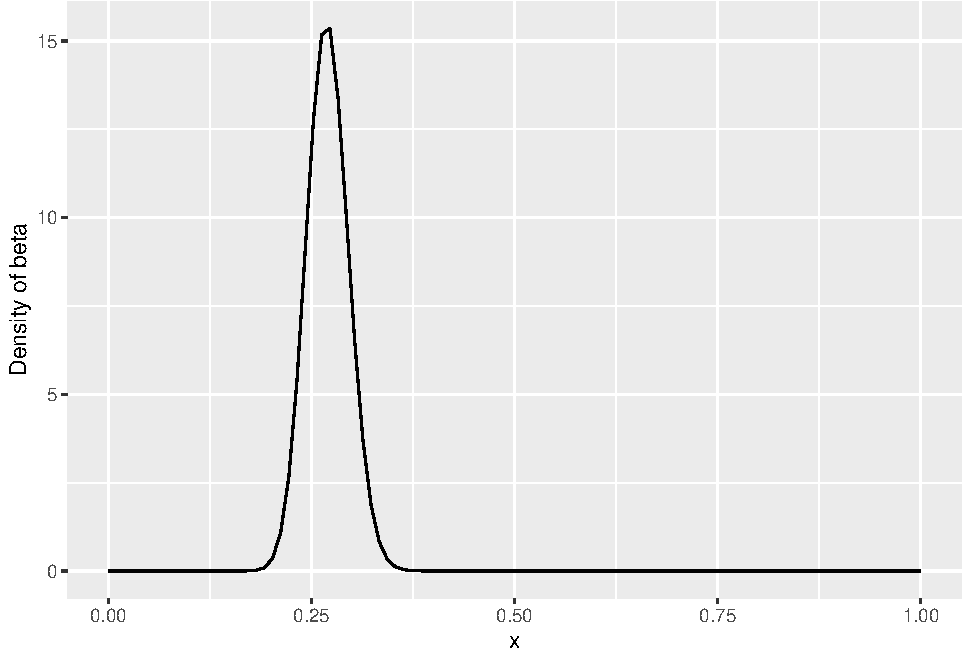
\includegraphics{datadown_files/figure-latex/beta-1.pdf}

\hypertarget{ux4e3aux4ec0ux4e48ux51fbux7403ux7684ux6982ux7387ux5206ux5e03ux7b26ux5408ux8d1dux5854ux5206ux5e03}{%
\section{为什么击球的概率分布符合贝塔分布?}\label{ux4e3aux4ec0ux4e48ux51fbux7403ux7684ux6982ux7387ux5206ux5e03ux7b26ux5408ux8d1dux5854ux5206ux5e03}}

\begin{itemize}
\tightlist
\item
  设想球员A打了一个球打中了,那么在没有先验知识的情况下我会认为他击中概率为1
\item
  这个球员又打中了一个球,那么还是1
\item
  但第三个没打中,我们会认为他击中概率是0吗?
\item
  一般而言,这类连续击球问题可以用二项分布来描述,例如10个球打中8个的概率,我们假设这个击球概率为q,那么这个概率应该是个q的函数:
\end{itemize}

\[f(q) \propto q^a(1-q)^b\]

\begin{itemize}
\tightlist
\item
  q对于一个实际问题是确定的常数,所以出现这个场景的概率实际上是a与b的函数
\item
  为了保障这个概率函数累积为1,需要除一个跟a与b有关的数
\item
  这个数可以用贝塔函数\(B(a,b)\)来表示,数学证明\href{https://en.wikipedia.org/wiki/Conjugate_prior\#Example}{略}
\item
  如果接着打了一个中了,那么如何更新这个概率?
\item
  根据贝叶斯公式,最后推导出的结果如下:
\end{itemize}

\[Beta(\alpha+1,\beta+0)\]

\begin{itemize}
\tightlist
\item
  那么我们对这个击球率的估计就略高了一点,这是贝塔分布的神奇之处,形式非常简单,理解也很直观
\end{itemize}

\hypertarget{ux5148ux9a8cux4e0eux540eux9a8c}{%
\section{先验与后验}\label{ux5148ux9a8cux4e0eux540eux9a8c}}

\begin{itemize}
\tightlist
\item
  如果我们后续观察的击球少,那么不太容易影响到对概率的先验估计
\end{itemize}

\begin{Shaded}
\begin{Highlighting}[]
\NormalTok{x <-}\StringTok{ }\KeywordTok{seq}\NormalTok{(}\DecValTok{0}\NormalTok{,}\DecValTok{1}\NormalTok{,}\DataTypeTok{length=}\DecValTok{100}\NormalTok{)}
\NormalTok{db <-}\StringTok{ }\KeywordTok{dbeta}\NormalTok{(x, }\DecValTok{81}\OperatorTok{+}\DecValTok{1}\NormalTok{, }\DecValTok{219}\NormalTok{)}
\KeywordTok{ggplot}\NormalTok{() }\OperatorTok{+}\StringTok{ }\KeywordTok{geom_line}\NormalTok{(}\KeywordTok{aes}\NormalTok{(x,db)) }\OperatorTok{+}\StringTok{ }\KeywordTok{ylab}\NormalTok{(}\StringTok{"Density of beta"}\NormalTok{)}
\end{Highlighting}
\end{Shaded}

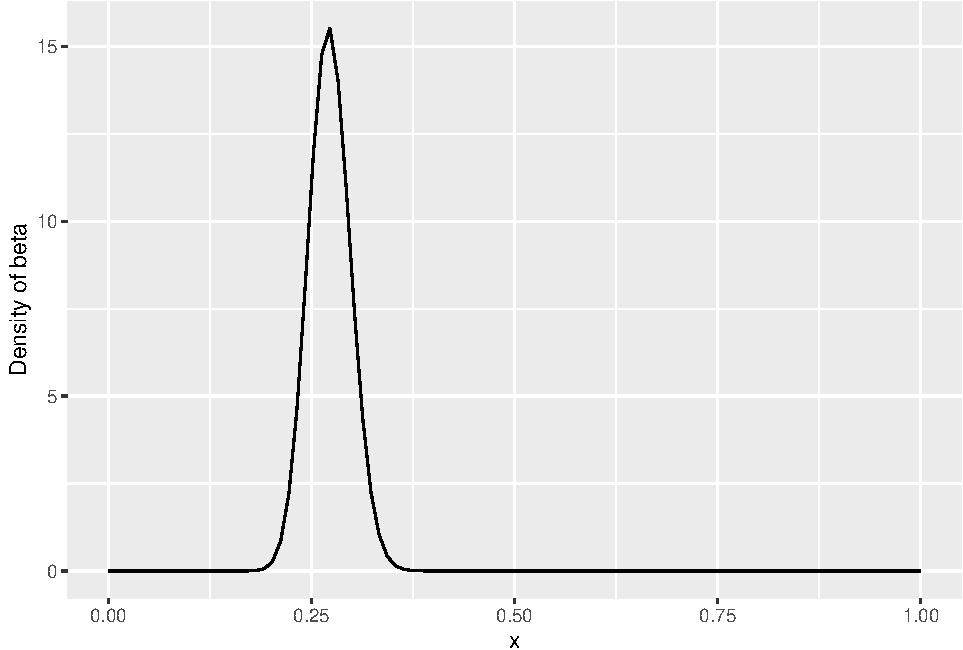
\includegraphics{datadown_files/figure-latex/beta1-1.pdf}

\begin{itemize}
\tightlist
\item
  如果后续观察了大量的击球都中了,那么概率会偏向后面数据量的那一部分
\end{itemize}

\begin{Shaded}
\begin{Highlighting}[]
\NormalTok{x <-}\StringTok{ }\KeywordTok{seq}\NormalTok{(}\DecValTok{0}\NormalTok{,}\DecValTok{1}\NormalTok{,}\DataTypeTok{length=}\DecValTok{100}\NormalTok{)}
\NormalTok{db <-}\StringTok{ }\KeywordTok{dbeta}\NormalTok{(x, }\DecValTok{81}\OperatorTok{+}\DecValTok{1000}\NormalTok{, }\DecValTok{219}\NormalTok{)}
\KeywordTok{ggplot}\NormalTok{() }\OperatorTok{+}\StringTok{ }\KeywordTok{geom_line}\NormalTok{(}\KeywordTok{aes}\NormalTok{(x,db)) }\OperatorTok{+}\StringTok{ }\KeywordTok{ylab}\NormalTok{(}\StringTok{"Density of beta"}\NormalTok{)}
\end{Highlighting}
\end{Shaded}

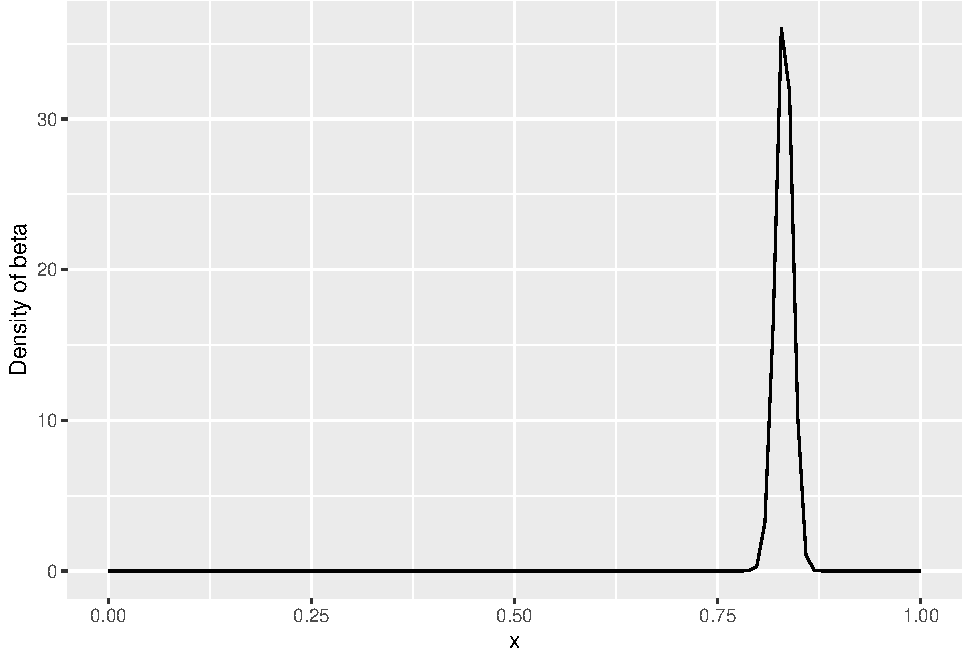
\includegraphics{datadown_files/figure-latex/beta2-1.pdf}

\begin{itemize}
\item
  这是贝叶斯分析的核心思想,通过证据更新经验
\item
  最后得到的均值(后验0.83)一定是介于经验值(先验0.27)与证据值(全击中就是1)之间
\item
  贝塔分布天然适合描述一个对概率的估计场景
\item
  另一种不那么严谨的理解方法是如果一个概率是稳定的,那么多次实验的结果差别不会太大,则有:
\end{itemize}

\[\frac{a}{b} = \frac{c}{d} = \frac{a+b}{c+d}\]

\begin{itemize}
\tightlist
\item
  如果每次实验的概率持平,那么不存在不确定度;但如果前面实验的次数少而后面实验的次数多,那么概率会偏重于后面,这就是贝塔分布想说明的事
\end{itemize}

\hypertarget{ux7ecfux9a8cux8d1dux53f6ux65af}{%
\section{经验贝叶斯}\label{ux7ecfux9a8cux8d1dux53f6ux65af}}

\begin{itemize}
\item
  对于两个球员,一个打了10个球中了4个,另一个打了1000个球中了300个,一般击中概率0.2,你会选哪一个?
\item
  我们对于小样本量的统计推断会有天然的不信任,如何通过统计量来描述?
\item
  下面用MLB的数据说明,首先提取出球员的击球数据:
\end{itemize}

\begin{Shaded}
\begin{Highlighting}[]
\KeywordTok{library}\NormalTok{(dplyr)}
\KeywordTok{library}\NormalTok{(tidyr)}
\KeywordTok{library}\NormalTok{(Lahman)}
\CommentTok{# 拿到击球数据}
\NormalTok{career <-}\StringTok{ }\NormalTok{Batting }\OperatorTok
\StringTok{  }\KeywordTok{filter}\NormalTok{(AB }\OperatorTok{>}\StringTok{ }\DecValTok{0}\NormalTok{) }\OperatorTok
\StringTok{  }\KeywordTok{anti_join}\NormalTok{(Pitching, }\DataTypeTok{by =} \StringTok{"playerID"}\NormalTok{) }\OperatorTok
\StringTok{  }\KeywordTok{group_by}\NormalTok{(playerID) }\OperatorTok
\StringTok{  }\KeywordTok{summarize}\NormalTok{(}\DataTypeTok{H =} \KeywordTok{sum}\NormalTok{(H), }\DataTypeTok{AB =} \KeywordTok{sum}\NormalTok{(AB)) }\OperatorTok
\StringTok{  }\KeywordTok{mutate}\NormalTok{(}\DataTypeTok{average =}\NormalTok{ H }\OperatorTok{/}\StringTok{ }\NormalTok{AB)}

\CommentTok{# 把ID换成球员名字}
\NormalTok{career <-}\StringTok{ }\NormalTok{Master }\OperatorTok
\StringTok{  }\KeywordTok{tbl_df}\NormalTok{() }\OperatorTok
\StringTok{  }\NormalTok{dplyr}\OperatorTok{::}\KeywordTok{select}\NormalTok{(playerID, nameFirst, nameLast) }\OperatorTok
\StringTok{  }\KeywordTok{unite}\NormalTok{(name, nameFirst, nameLast, }\DataTypeTok{sep =} \StringTok{" "}\NormalTok{) }\OperatorTok
\StringTok{  }\KeywordTok{inner_join}\NormalTok{(career, }\DataTypeTok{by =} \StringTok{"playerID"}\NormalTok{) }\OperatorTok
\StringTok{  }\NormalTok{dplyr}\OperatorTok{::}\KeywordTok{select}\NormalTok{(}\OperatorTok{-}\NormalTok{playerID)}
\CommentTok{# 展示数据}
\NormalTok{career}
\end{Highlighting}
\end{Shaded}

\begin{verbatim}
## # A tibble: 9,670 x 4
##    name                  H    AB average
##    <chr>             <int> <int>   <dbl>
##  1 Hank Aaron         3771 12364  0.305 
##  2 Tommie Aaron        216   944  0.229 
##  3 Andy Abad             2    21  0.0952
##  4 John Abadie          11    49  0.224 
##  5 Ed Abbaticchio      772  3044  0.254 
##  6 Fred Abbott         107   513  0.209 
##  7 Jeff Abbott         157   596  0.263 
##  8 Kurt Abbott         523  2044  0.256 
##  9 Ody Abbott           13    70  0.186 
## 10 Frank Abercrombie     0     4  0     
## # ... with 9,660 more rows
\end{verbatim}

\begin{Shaded}
\begin{Highlighting}[]
\CommentTok{# 击球前5}
\NormalTok{career }\OperatorTok
\StringTok{  }\KeywordTok{arrange}\NormalTok{(}\KeywordTok{desc}\NormalTok{(average)) }\OperatorTok
\StringTok{  }\KeywordTok{head}\NormalTok{(}\DecValTok{5}\NormalTok{) }\OperatorTok
\StringTok{  }\KeywordTok{kable}\NormalTok{()}
\end{Highlighting}
\end{Shaded}

\begin{tabular}{l|r|r|r}
\hline
name & H & AB & average\\
\hline
Jeff Banister & 1 & 1 & 1\\
\hline
Doc Bass & 1 & 1 & 1\\
\hline
Steve Biras & 2 & 2 & 1\\
\hline
C. B. Burns & 1 & 1 & 1\\
\hline
Jackie Gallagher & 1 & 1 & 1\\
\hline
\end{tabular}

\begin{Shaded}
\begin{Highlighting}[]
\CommentTok{# 击球后5}
\NormalTok{career }\OperatorTok
\StringTok{  }\KeywordTok{arrange}\NormalTok{(average) }\OperatorTok
\StringTok{  }\KeywordTok{head}\NormalTok{(}\DecValTok{5}\NormalTok{) }\OperatorTok
\StringTok{  }\KeywordTok{kable}\NormalTok{()}
\end{Highlighting}
\end{Shaded}

\begin{tabular}{l|r|r|r}
\hline
name & H & AB & average\\
\hline
Frank Abercrombie & 0 & 4 & 0\\
\hline
Horace Allen & 0 & 7 & 0\\
\hline
Pete Allen & 0 & 4 & 0\\
\hline
Walter Alston & 0 & 1 & 0\\
\hline
Bill Andrus & 0 & 9 & 0\\
\hline
\end{tabular}

\begin{itemize}
\item
  如果仅考虑击球率会把很多板凳球员与运气球员包括进来,一个先验概率分布很有必要
\item
  那么考虑下如何得到,经验贝叶斯方法认为如果估计一个个体的参数,那么这个个体所在的整体的概率分布可作为先验概率分布
\item
  这个先验概率分布可以直接从数据中得到,然后我们要用极大似然或矩估计的方法拿到贝塔分布的两个参数:
\end{itemize}

\begin{Shaded}
\begin{Highlighting}[]
\NormalTok{career_filtered <-}\StringTok{ }\NormalTok{career }\OperatorTok
\StringTok{    }\KeywordTok{filter}\NormalTok{(AB }\OperatorTok{>=}\StringTok{ }\DecValTok{500}\NormalTok{)}

\NormalTok{m <-}\StringTok{ }\NormalTok{MASS}\OperatorTok{::}\KeywordTok{fitdistr}\NormalTok{(career_filtered}\OperatorTok{$}\NormalTok{average, dbeta,}
                    \DataTypeTok{start =} \KeywordTok{list}\NormalTok{(}\DataTypeTok{shape1 =} \DecValTok{1}\NormalTok{, }\DataTypeTok{shape2 =} \DecValTok{10}\NormalTok{))}

\NormalTok{alpha0 <-}\StringTok{ }\NormalTok{m}\OperatorTok{$}\NormalTok{estimate[}\DecValTok{1}\NormalTok{]}
\NormalTok{beta0 <-}\StringTok{ }\NormalTok{m}\OperatorTok{$}\NormalTok{estimate[}\DecValTok{2}\NormalTok{]}

\CommentTok{# 看下拟合效果}

\KeywordTok{ggplot}\NormalTok{(career_filtered) }\OperatorTok{+}
\StringTok{  }\KeywordTok{geom_histogram}\NormalTok{(}\KeywordTok{aes}\NormalTok{(average, }\DataTypeTok{y =}\NormalTok{ ..density..), }\DataTypeTok{binwidth =} \FloatTok{.005}\NormalTok{) }\OperatorTok{+}
\StringTok{  }\KeywordTok{stat_function}\NormalTok{(}\DataTypeTok{fun =} \ControlFlowTok{function}\NormalTok{(x) }\KeywordTok{dbeta}\NormalTok{(x, alpha0, beta0), }\DataTypeTok{color =} \StringTok{"red"}\NormalTok{,}
                \DataTypeTok{size =} \DecValTok{1}\NormalTok{) }\OperatorTok{+}
\StringTok{  }\KeywordTok{xlab}\NormalTok{(}\StringTok{"Batting average"}\NormalTok{)}
\end{Highlighting}
\end{Shaded}

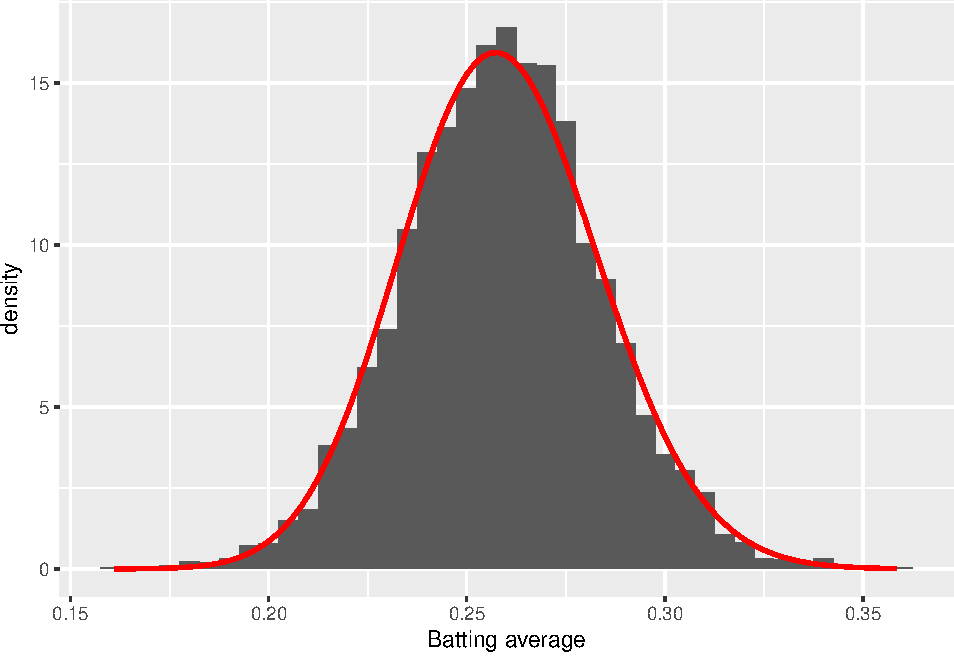
\includegraphics{datadown_files/figure-latex/ebayes-1.pdf}

\hypertarget{ux4eceux6574ux4f53ux5230ux4e2aux4eba}{%
\section{从整体到个人}\label{ux4eceux6574ux4f53ux5230ux4e2aux4eba}}

\begin{itemize}
\item
  当我们估计个人的击球率时,整体可以作为先验函数,个人的数据可以通过贝塔分布更新到个体
\item
  那么如果一个人数据少,我们倾向于认为他是平均水平;数据多则认为符合个人表现
\item
  这事实上是一个分层结构,经验贝叶斯推断里隐含了这么一个从整体到个人的过程
\end{itemize}

\begin{Shaded}
\begin{Highlighting}[]
\NormalTok{career_eb <-}\StringTok{ }\NormalTok{career }\OperatorTok
\StringTok{    }\KeywordTok{mutate}\NormalTok{(}\DataTypeTok{eb_estimate =}\NormalTok{ (H }\OperatorTok{+}\StringTok{ }\NormalTok{alpha0) }\OperatorTok{/}\StringTok{ }\NormalTok{(AB }\OperatorTok{+}\StringTok{ }\NormalTok{alpha0 }\OperatorTok{+}\StringTok{ }\NormalTok{beta0))}
\CommentTok{# 击球率高}
\NormalTok{career_eb }\OperatorTok
\StringTok{  }\KeywordTok{arrange}\NormalTok{(}\KeywordTok{desc}\NormalTok{(eb_estimate)) }\OperatorTok
\StringTok{  }\KeywordTok{head}\NormalTok{(}\DecValTok{5}\NormalTok{) }\OperatorTok
\StringTok{  }\KeywordTok{kable}\NormalTok{()}
\end{Highlighting}
\end{Shaded}

\begin{tabular}{l|r|r|r|r}
\hline
name & H & AB & average & eb\_estimate\\
\hline
Rogers Hornsby & 2930 & 8173 & 0.358 & 0.355\\
\hline
Shoeless Joe Jackson & 1772 & 4981 & 0.356 & 0.350\\
\hline
Ed Delahanty & 2597 & 7510 & 0.346 & 0.342\\
\hline
Billy Hamilton & 2164 & 6283 & 0.344 & 0.340\\
\hline
Harry Heilmann & 2660 & 7787 & 0.342 & 0.338\\
\hline
\end{tabular}

\begin{Shaded}
\begin{Highlighting}[]
\CommentTok{# 击球率低}
\NormalTok{career_eb }\OperatorTok
\StringTok{  }\KeywordTok{arrange}\NormalTok{(eb_estimate) }\OperatorTok
\StringTok{  }\KeywordTok{head}\NormalTok{(}\DecValTok{5}\NormalTok{) }\OperatorTok
\StringTok{  }\KeywordTok{kable}\NormalTok{()}
\end{Highlighting}
\end{Shaded}

\begin{tabular}{l|r|r|r|r}
\hline
name & H & AB & average & eb\_estimate\\
\hline
Bill Bergen & 516 & 3028 & 0.170 & 0.179\\
\hline
Ray Oyler & 221 & 1265 & 0.175 & 0.191\\
\hline
John Vukovich & 90 & 559 & 0.161 & 0.196\\
\hline
John Humphries & 52 & 364 & 0.143 & 0.196\\
\hline
George Baker & 74 & 474 & 0.156 & 0.196\\
\hline
\end{tabular}

\begin{Shaded}
\begin{Highlighting}[]
\CommentTok{# 整体估计}
\KeywordTok{ggplot}\NormalTok{(career_eb, }\KeywordTok{aes}\NormalTok{(average, eb_estimate, }\DataTypeTok{color =}\NormalTok{ AB)) }\OperatorTok{+}
\StringTok{  }\KeywordTok{geom_hline}\NormalTok{(}\DataTypeTok{yintercept =}\NormalTok{ alpha0 }\OperatorTok{/}\StringTok{ }\NormalTok{(alpha0 }\OperatorTok{+}\StringTok{ }\NormalTok{beta0), }\DataTypeTok{color =} \StringTok{"red"}\NormalTok{, }\DataTypeTok{lty =} \DecValTok{2}\NormalTok{) }\OperatorTok{+}
\StringTok{  }\KeywordTok{geom_point}\NormalTok{() }\OperatorTok{+}
\StringTok{  }\KeywordTok{geom_abline}\NormalTok{(}\DataTypeTok{color =} \StringTok{"red"}\NormalTok{) }\OperatorTok{+}
\StringTok{  }\KeywordTok{scale_colour_gradient}\NormalTok{(}\DataTypeTok{trans =} \StringTok{"log"}\NormalTok{, }\DataTypeTok{breaks =} \DecValTok{10} \OperatorTok{^}\StringTok{ }\NormalTok{(}\DecValTok{1}\OperatorTok{:}\DecValTok{5}\NormalTok{)) }\OperatorTok{+}
\StringTok{  }\KeywordTok{xlab}\NormalTok{(}\StringTok{"Batting average"}\NormalTok{) }\OperatorTok{+}
\StringTok{  }\KeywordTok{ylab}\NormalTok{(}\StringTok{"Empirical Bayes batting average"}\NormalTok{)}
\end{Highlighting}
\end{Shaded}

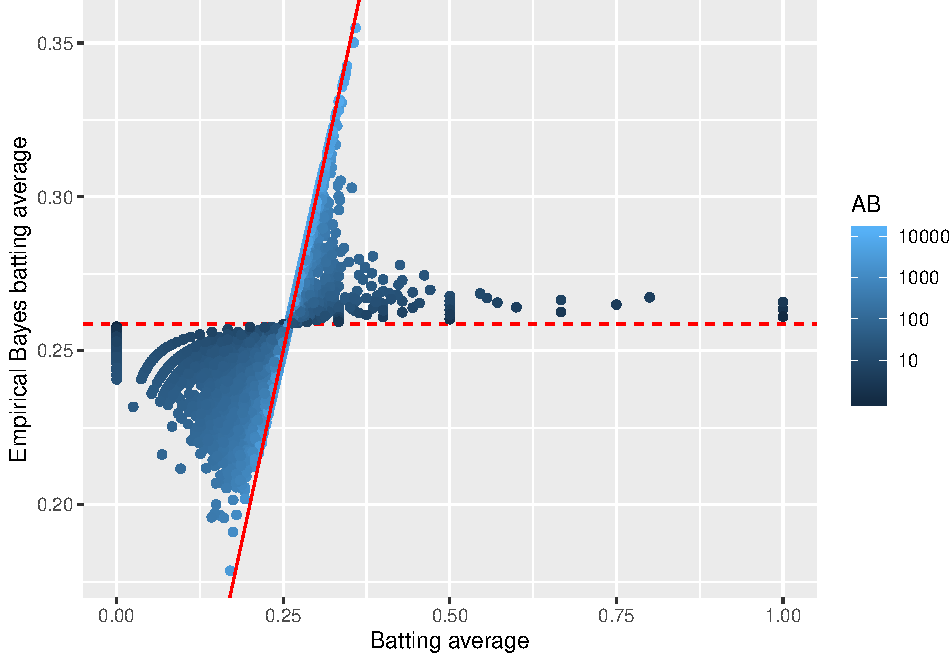
\includegraphics{datadown_files/figure-latex/ebayes2-1.pdf}

\begin{itemize}
\item
  数据点多会收缩到\(x=y\),也就是个人的击球率;数据点少则回归到整体击球率
\item
  这就是经验贝叶斯方法的全貌:先估计整体的参数,然后把整体参数作为先验概率估计个人参数
\end{itemize}

\hypertarget{ux53efux4fe1ux533aux95f4ux4e0eux7f6eux4fe1ux533aux95f4}{%
\section{可信区间与置信区间}\label{ux53efux4fe1ux533aux95f4ux4e0eux7f6eux4fe1ux533aux95f4}}

\begin{itemize}
\item
  经验贝叶斯可以给出点估计,但现实中我们可能更关心区间估计
\item
  一般这类区间估计可以用二项式比例估计来进行,不过没有先验经验的限制置信区间大到没意义
\item
  经验贝叶斯会给出一个后验分布,这个分布可以用来求可信区间
\end{itemize}

\begin{Shaded}
\begin{Highlighting}[]
\KeywordTok{library}\NormalTok{(broom)}
\CommentTok{# 给出后验分布}
\NormalTok{career <-}\StringTok{ }\NormalTok{Batting }\OperatorTok
\StringTok{  }\KeywordTok{filter}\NormalTok{(AB }\OperatorTok{>}\StringTok{ }\DecValTok{0}\NormalTok{) }\OperatorTok
\StringTok{  }\KeywordTok{anti_join}\NormalTok{(Pitching, }\DataTypeTok{by =} \StringTok{"playerID"}\NormalTok{) }\OperatorTok
\StringTok{  }\KeywordTok{group_by}\NormalTok{(playerID) }\OperatorTok
\StringTok{  }\KeywordTok{summarize}\NormalTok{(}\DataTypeTok{H =} \KeywordTok{sum}\NormalTok{(H), }\DataTypeTok{AB =} \KeywordTok{sum}\NormalTok{(AB)) }\OperatorTok
\StringTok{  }\KeywordTok{mutate}\NormalTok{(}\DataTypeTok{average =}\NormalTok{ H }\OperatorTok{/}\StringTok{ }\NormalTok{AB)}

\NormalTok{career <-}\StringTok{ }\NormalTok{Master }\OperatorTok
\StringTok{  }\KeywordTok{tbl_df}\NormalTok{() }\OperatorTok
\StringTok{  }\NormalTok{dplyr}\OperatorTok{::}\KeywordTok{select}\NormalTok{(playerID, nameFirst, nameLast) }\OperatorTok
\StringTok{  }\KeywordTok{unite}\NormalTok{(name, nameFirst, nameLast, }\DataTypeTok{sep =} \StringTok{" "}\NormalTok{) }\OperatorTok
\StringTok{  }\KeywordTok{inner_join}\NormalTok{(career, }\DataTypeTok{by =} \StringTok{"playerID"}\NormalTok{)}

\NormalTok{career0 <-}\StringTok{ }\NormalTok{Batting }\OperatorTok
\StringTok{  }\KeywordTok{filter}\NormalTok{(AB }\OperatorTok{>}\StringTok{ }\DecValTok{0}\NormalTok{) }\OperatorTok
\StringTok{  }\KeywordTok{anti_join}\NormalTok{(Pitching, }\DataTypeTok{by =} \StringTok{"playerID"}\NormalTok{) }\OperatorTok
\StringTok{  }\KeywordTok{group_by}\NormalTok{(playerID) }\OperatorTok
\StringTok{  }\KeywordTok{summarize}\NormalTok{(}\DataTypeTok{H =} \KeywordTok{sum}\NormalTok{(H), }\DataTypeTok{AB =} \KeywordTok{sum}\NormalTok{(AB), }\DataTypeTok{year =} \KeywordTok{mean}\NormalTok{(yearID)) }\OperatorTok
\StringTok{  }\KeywordTok{mutate}\NormalTok{(}\DataTypeTok{average =}\NormalTok{ H }\OperatorTok{/}\StringTok{ }\NormalTok{AB)}

\NormalTok{career2 <-}\StringTok{ }\NormalTok{Master }\OperatorTok
\StringTok{  }\KeywordTok{tbl_df}\NormalTok{() }\OperatorTok
\StringTok{  }\NormalTok{dplyr}\OperatorTok{::}\KeywordTok{select}\NormalTok{(playerID, nameFirst, nameLast, bats) }\OperatorTok
\StringTok{  }\KeywordTok{unite}\NormalTok{(name, nameFirst, nameLast, }\DataTypeTok{sep =} \StringTok{" "}\NormalTok{) }\OperatorTok
\StringTok{  }\KeywordTok{inner_join}\NormalTok{(career0, }\DataTypeTok{by =} \StringTok{"playerID"}\NormalTok{)}

\NormalTok{career_eb <-}\StringTok{ }\NormalTok{career }\OperatorTok
\StringTok{    }\KeywordTok{mutate}\NormalTok{(}\DataTypeTok{eb_estimate =}\NormalTok{ (H }\OperatorTok{+}\StringTok{ }\NormalTok{alpha0) }\OperatorTok{/}\StringTok{ }\NormalTok{(AB }\OperatorTok{+}\StringTok{ }\NormalTok{alpha0 }\OperatorTok{+}\StringTok{ }\NormalTok{beta0))}
\NormalTok{career_eb <-}\StringTok{ }\NormalTok{career_eb }\OperatorTok
\StringTok{    }\KeywordTok{mutate}\NormalTok{(}\DataTypeTok{alpha1 =}\NormalTok{ H }\OperatorTok{+}\StringTok{ }\NormalTok{alpha0,}
           \DataTypeTok{beta1 =}\NormalTok{ AB }\OperatorTok{-}\StringTok{ }\NormalTok{H }\OperatorTok{+}\StringTok{ }\NormalTok{beta0)}
\CommentTok{# 提取洋基队的数据}
\NormalTok{yankee_}\DecValTok{1998}\NormalTok{ <-}\StringTok{ }\KeywordTok{c}\NormalTok{(}\StringTok{"brosisc01"}\NormalTok{, }\StringTok{"jeterde01"}\NormalTok{, }\StringTok{"knoblch01"}\NormalTok{, }\StringTok{"martiti02"}\NormalTok{, }\StringTok{"posadjo01"}\NormalTok{, }\StringTok{"strawda01"}\NormalTok{, }\StringTok{"willibe02"}\NormalTok{)}

\NormalTok{yankee_}\DecValTok{1998}\NormalTok{_career <-}\StringTok{ }\NormalTok{career_eb }\OperatorTok
\StringTok{    }\KeywordTok{filter}\NormalTok{(playerID }\OperatorTok\StringTok{ }\NormalTok{yankee_}\DecValTok{1998}\NormalTok{)}

\CommentTok{# 提取可信区间}
\NormalTok{yankee_}\DecValTok{1998}\NormalTok{_career <-}\StringTok{ }\NormalTok{yankee_}\DecValTok{1998}\NormalTok{_career }\OperatorTok
\StringTok{    }\KeywordTok{mutate}\NormalTok{(}\DataTypeTok{low  =} \KeywordTok{qbeta}\NormalTok{(.}\DecValTok{025}\NormalTok{, alpha1, beta1),}
           \DataTypeTok{high =} \KeywordTok{qbeta}\NormalTok{(.}\DecValTok{975}\NormalTok{, alpha1, beta1))}
\NormalTok{yankee_}\DecValTok{1998}\NormalTok{_career }\OperatorTok
\StringTok{    }\NormalTok{dplyr}\OperatorTok{::}\KeywordTok{select}\NormalTok{(}\OperatorTok{-}\NormalTok{alpha1, }\OperatorTok{-}\NormalTok{beta1, }\OperatorTok{-}\NormalTok{eb_estimate) }\OperatorTok
\StringTok{    }\NormalTok{knitr}\OperatorTok{::}\KeywordTok{kable}\NormalTok{()}
\end{Highlighting}
\end{Shaded}

\begin{tabular}{l|l|r|r|r|r|r}
\hline
playerID & name & H & AB & average & low & high\\
\hline
brosisc01 & Scott Brosius & 1001 & 3889 & 0.257 & 0.244 & 0.271\\
\hline
jeterde01 & Derek Jeter & 3465 & 11195 & 0.310 & 0.300 & 0.317\\
\hline
knoblch01 & Chuck Knoblauch & 1839 & 6366 & 0.289 & 0.277 & 0.298\\
\hline
martiti02 & Tino Martinez & 1925 & 7111 & 0.271 & 0.260 & 0.280\\
\hline
posadjo01 & Jorge Posada & 1664 & 6092 & 0.273 & 0.262 & 0.283\\
\hline
strawda01 & Darryl Strawberry & 1401 & 5418 & 0.259 & 0.247 & 0.270\\
\hline
willibe02 & Bernie Williams & 2336 & 7869 & 0.297 & 0.286 & 0.305\\
\hline
\end{tabular}

\begin{Shaded}
\begin{Highlighting}[]
\CommentTok{# 绘制可信区间}
\NormalTok{yankee_}\DecValTok{1998}\NormalTok{_career }\OperatorTok
\StringTok{    }\KeywordTok{mutate}\NormalTok{(}\DataTypeTok{name =} \KeywordTok{reorder}\NormalTok{(name, average)) }\OperatorTok
\StringTok{    }\KeywordTok{ggplot}\NormalTok{(}\KeywordTok{aes}\NormalTok{(average, name)) }\OperatorTok{+}
\StringTok{    }\KeywordTok{geom_point}\NormalTok{() }\OperatorTok{+}
\StringTok{    }\KeywordTok{geom_errorbarh}\NormalTok{(}\KeywordTok{aes}\NormalTok{(}\DataTypeTok{xmin =}\NormalTok{ low, }\DataTypeTok{xmax =}\NormalTok{ high)) }\OperatorTok{+}
\StringTok{    }\KeywordTok{geom_vline}\NormalTok{(}\DataTypeTok{xintercept =}\NormalTok{ alpha0 }\OperatorTok{/}\StringTok{ }\NormalTok{(alpha0 }\OperatorTok{+}\StringTok{ }\NormalTok{beta0), }\DataTypeTok{color =} \StringTok{"red"}\NormalTok{, }\DataTypeTok{lty =} \DecValTok{2}\NormalTok{) }\OperatorTok{+}
\StringTok{    }\KeywordTok{xlab}\NormalTok{(}\StringTok{"Estimated batting average (w/ 95% interval)"}\NormalTok{) }\OperatorTok{+}
\StringTok{    }\KeywordTok{ylab}\NormalTok{(}\StringTok{"Player"}\NormalTok{)}
\end{Highlighting}
\end{Shaded}

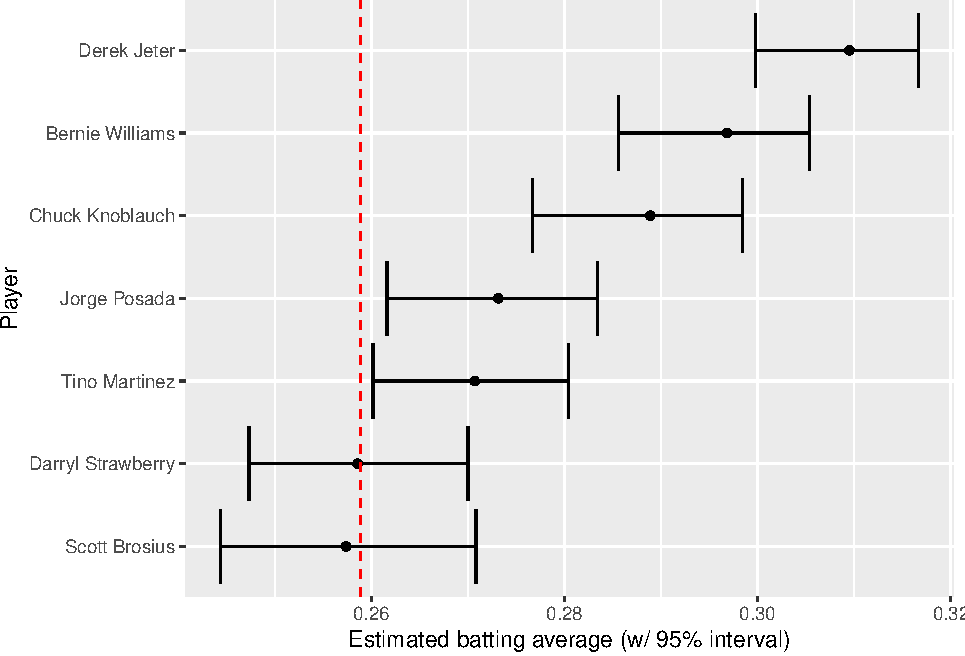
\includegraphics{datadown_files/figure-latex/ci-1.pdf}

\begin{Shaded}
\begin{Highlighting}[]
\CommentTok{# 对比置信区间与可信区间}
\NormalTok{career_eb <-}\StringTok{ }\NormalTok{career_eb }\OperatorTok
\StringTok{    }\KeywordTok{mutate}\NormalTok{(}\DataTypeTok{low =} \KeywordTok{qbeta}\NormalTok{(.}\DecValTok{025}\NormalTok{, alpha1, beta1),}
           \DataTypeTok{high =} \KeywordTok{qbeta}\NormalTok{(.}\DecValTok{975}\NormalTok{, alpha1, beta1))}

\KeywordTok{set.seed}\NormalTok{(}\DecValTok{2016}\NormalTok{)}

\NormalTok{some <-}\StringTok{ }\NormalTok{career_eb }\OperatorTok
\StringTok{    }\KeywordTok{sample_n}\NormalTok{(}\DecValTok{20}\NormalTok{) }\OperatorTok
\StringTok{    }\KeywordTok{mutate}\NormalTok{(}\DataTypeTok{name =} \KeywordTok{paste0}\NormalTok{(name, }\StringTok{" ("}\NormalTok{, H, }\StringTok{"/"}\NormalTok{, AB, }\StringTok{")"}\NormalTok{))}

\NormalTok{frequentist <-}\StringTok{ }\NormalTok{some }\OperatorTok
\StringTok{    }\KeywordTok{group_by}\NormalTok{(playerID, name, AB) }\OperatorTok
\StringTok{    }\KeywordTok{do}\NormalTok{(}\KeywordTok{tidy}\NormalTok{(}\KeywordTok{binom.test}\NormalTok{(.}\OperatorTok{$}\NormalTok{H, .}\OperatorTok{$}\NormalTok{AB))) }\OperatorTok
\StringTok{    }\NormalTok{dplyr}\OperatorTok{::}\KeywordTok{select}\NormalTok{(playerID, name, estimate, }\DataTypeTok{low =}\NormalTok{ conf.low, }\DataTypeTok{high =}\NormalTok{ conf.high) }\OperatorTok
\StringTok{    }\KeywordTok{mutate}\NormalTok{(}\DataTypeTok{method =} \StringTok{"Confidence"}\NormalTok{)}

\NormalTok{bayesian <-}\StringTok{ }\NormalTok{some }\OperatorTok
\StringTok{    }\NormalTok{dplyr}\OperatorTok{::}\KeywordTok{select}\NormalTok{(playerID, name, AB, }\DataTypeTok{estimate =}\NormalTok{ eb_estimate,}
           \DataTypeTok{low =}\NormalTok{ low, }\DataTypeTok{high =}\NormalTok{ high) }\OperatorTok
\StringTok{    }\KeywordTok{mutate}\NormalTok{(}\DataTypeTok{method =} \StringTok{"Credible"}\NormalTok{)}

\NormalTok{combined <-}\StringTok{ }\KeywordTok{bind_rows}\NormalTok{(frequentist, bayesian)}

\NormalTok{combined }\OperatorTok
\StringTok{    }\KeywordTok{mutate}\NormalTok{(}\DataTypeTok{name2 =} \KeywordTok{reorder}\NormalTok{(name, }\OperatorTok{-}\NormalTok{AB)) }\OperatorTok
\StringTok{    }\KeywordTok{ggplot}\NormalTok{(}\KeywordTok{aes}\NormalTok{(estimate, name2, }\DataTypeTok{color =}\NormalTok{ method, }\DataTypeTok{group =}\NormalTok{ method)) }\OperatorTok{+}
\StringTok{    }\KeywordTok{geom_point}\NormalTok{() }\OperatorTok{+}
\StringTok{    }\KeywordTok{geom_errorbarh}\NormalTok{(}\KeywordTok{aes}\NormalTok{(}\DataTypeTok{xmin =}\NormalTok{ low, }\DataTypeTok{xmax =}\NormalTok{ high)) }\OperatorTok{+}
\StringTok{    }\KeywordTok{geom_vline}\NormalTok{(}\DataTypeTok{xintercept =}\NormalTok{ alpha0 }\OperatorTok{/}\StringTok{ }\NormalTok{(alpha0 }\OperatorTok{+}\StringTok{ }\NormalTok{beta0), }\DataTypeTok{color =} \StringTok{"red"}\NormalTok{, }\DataTypeTok{lty =} \DecValTok{2}\NormalTok{) }\OperatorTok{+}
\StringTok{    }\KeywordTok{xlab}\NormalTok{(}\StringTok{"Estimated batting average"}\NormalTok{) }\OperatorTok{+}
\StringTok{    }\KeywordTok{ylab}\NormalTok{(}\StringTok{"Player"}\NormalTok{) }\OperatorTok{+}
\StringTok{    }\KeywordTok{labs}\NormalTok{(}\DataTypeTok{color =} \StringTok{""}\NormalTok{)}
\end{Highlighting}
\end{Shaded}

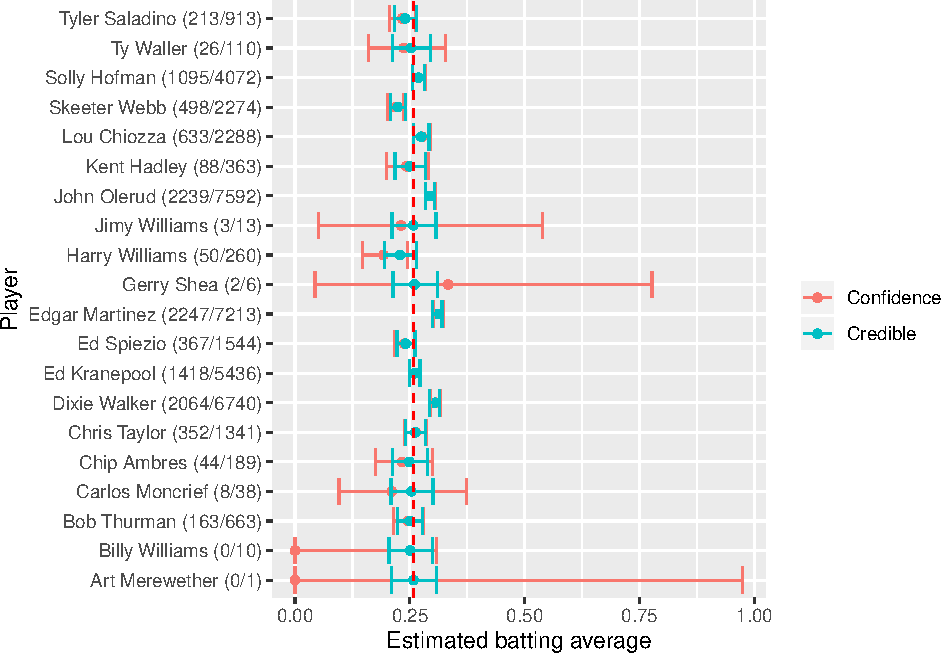
\includegraphics{datadown_files/figure-latex/ci-2.pdf}

\begin{itemize}
\tightlist
\item
  可信区间与置信区间很大的区别在于前者考虑了先验概率进而实现了区间的收缩,后者则可看作无先验贝塔分布给出的区间估计,频率学派目前没有很好的收缩区间估计的方法
\end{itemize}

\hypertarget{ux540eux9a8cux9519ux8befux7387}{%
\section{后验错误率}\label{ux540eux9a8cux9519ux8befux7387}}

\begin{itemize}
\tightlist
\item
  现实问题经常不局限于估计,而是侧重决策,例如如果一个球员的击球率高于某个值,他就可以进入名人堂(击球率大于0.3),这个决策常常伴随区间估计而不是简单的点估计
\end{itemize}

\begin{Shaded}
\begin{Highlighting}[]
\CommentTok{# 以 Hank Aaron 为例}
\NormalTok{career_eb }\OperatorTok
\StringTok{    }\KeywordTok{filter}\NormalTok{(name }\OperatorTok{==}\StringTok{ "Hank Aaron"}\NormalTok{) }\OperatorTok
\StringTok{    }\KeywordTok{do}\NormalTok{(}\KeywordTok{data_frame}\NormalTok{(}\DataTypeTok{x =} \KeywordTok{seq}\NormalTok{(.}\DecValTok{27}\NormalTok{, }\FloatTok{.33}\NormalTok{, }\FloatTok{.0002}\NormalTok{),}
                  \DataTypeTok{density =} \KeywordTok{dbeta}\NormalTok{(x, .}\OperatorTok{$}\NormalTok{alpha1, .}\OperatorTok{$}\NormalTok{beta1))) }\OperatorTok
\StringTok{    }\KeywordTok{ggplot}\NormalTok{(}\KeywordTok{aes}\NormalTok{(x, density)) }\OperatorTok{+}
\StringTok{    }\KeywordTok{geom_line}\NormalTok{() }\OperatorTok{+}
\StringTok{    }\KeywordTok{geom_ribbon}\NormalTok{(}\KeywordTok{aes}\NormalTok{(}\DataTypeTok{ymin =} \DecValTok{0}\NormalTok{, }\DataTypeTok{ymax =}\NormalTok{ density }\OperatorTok{*}\StringTok{ }\NormalTok{(x }\OperatorTok{<}\StringTok{ }\FloatTok{.3}\NormalTok{)),}
                \DataTypeTok{alpha =} \FloatTok{.1}\NormalTok{, }\DataTypeTok{fill =} \StringTok{"red"}\NormalTok{) }\OperatorTok{+}
\StringTok{    }\KeywordTok{geom_vline}\NormalTok{(}\DataTypeTok{color =} \StringTok{"red"}\NormalTok{, }\DataTypeTok{lty =} \DecValTok{2}\NormalTok{, }\DataTypeTok{xintercept =} \FloatTok{.3}\NormalTok{)}
\end{Highlighting}
\end{Shaded}

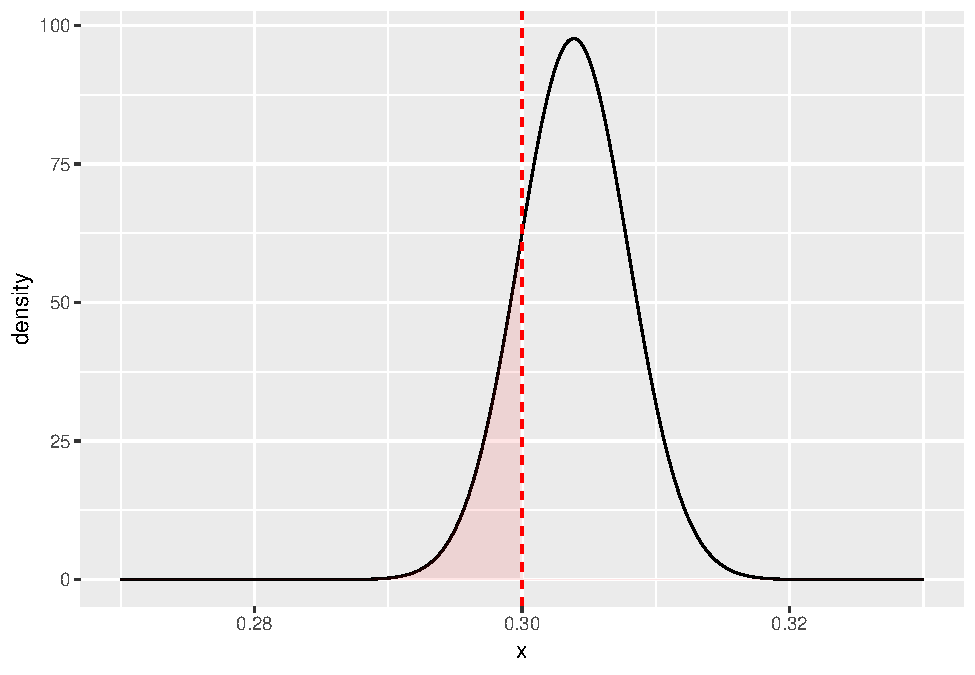
\includegraphics{datadown_files/figure-latex/lp-1.pdf}

\begin{Shaded}
\begin{Highlighting}[]
\CommentTok{# 提取该球员数据}
\NormalTok{career_eb }\OperatorTok\StringTok{ }\KeywordTok{filter}\NormalTok{(name }\OperatorTok{==}\StringTok{ "Hank Aaron"}\NormalTok{)}
\end{Highlighting}
\end{Shaded}

\begin{verbatim}
## # A tibble: 1 x 10
##   playerID  name       H    AB average eb_estimate alpha1 beta1   low  high
##   <chr>     <chr>  <int> <int>   <dbl>       <dbl>  <dbl> <dbl> <dbl> <dbl>
## 1 aaronha01 Hank ~  3771 12364   0.305       0.304  3851. 8821. 0.296 0.312
\end{verbatim}

\begin{Shaded}
\begin{Highlighting}[]
\CommentTok{# 计算其不进入名人堂的概率}
\KeywordTok{pbeta}\NormalTok{(.}\DecValTok{3}\NormalTok{, }\DecValTok{3850}\NormalTok{, }\DecValTok{8818}\NormalTok{)}
\end{Highlighting}
\end{Shaded}

\begin{verbatim}
## [1] 0.169
\end{verbatim}

\begin{itemize}
\item
  后验错误率(Posterior Error Probability)可类比经典假设检验中的显著性水平\(\alpha\)
\item
  后验包括率(Posterior Inclusion Probability)可类比经典假设检验中的置信水平\(1-\alpha\)
\end{itemize}

\begin{Shaded}
\begin{Highlighting}[]
\CommentTok{# 所有球员的后验错误率分布,大部分不超过0.3}
\NormalTok{career_eb <-}\StringTok{ }\NormalTok{career_eb }\OperatorTok
\StringTok{    }\KeywordTok{mutate}\NormalTok{(}\DataTypeTok{PEP =} \KeywordTok{pbeta}\NormalTok{(.}\DecValTok{3}\NormalTok{, alpha1, beta1))}
\KeywordTok{ggplot}\NormalTok{(career_eb, }\KeywordTok{aes}\NormalTok{(PEP)) }\OperatorTok{+}
\StringTok{    }\KeywordTok{geom_histogram}\NormalTok{(}\DataTypeTok{binwidth =} \FloatTok{.02}\NormalTok{) }\OperatorTok{+}
\StringTok{    }\KeywordTok{xlab}\NormalTok{(}\StringTok{"Posterior Error Probability (PEP)"}\NormalTok{) }\OperatorTok{+}
\StringTok{    }\KeywordTok{xlim}\NormalTok{(}\DecValTok{0}\NormalTok{, }\DecValTok{1}\NormalTok{)}
\end{Highlighting}
\end{Shaded}

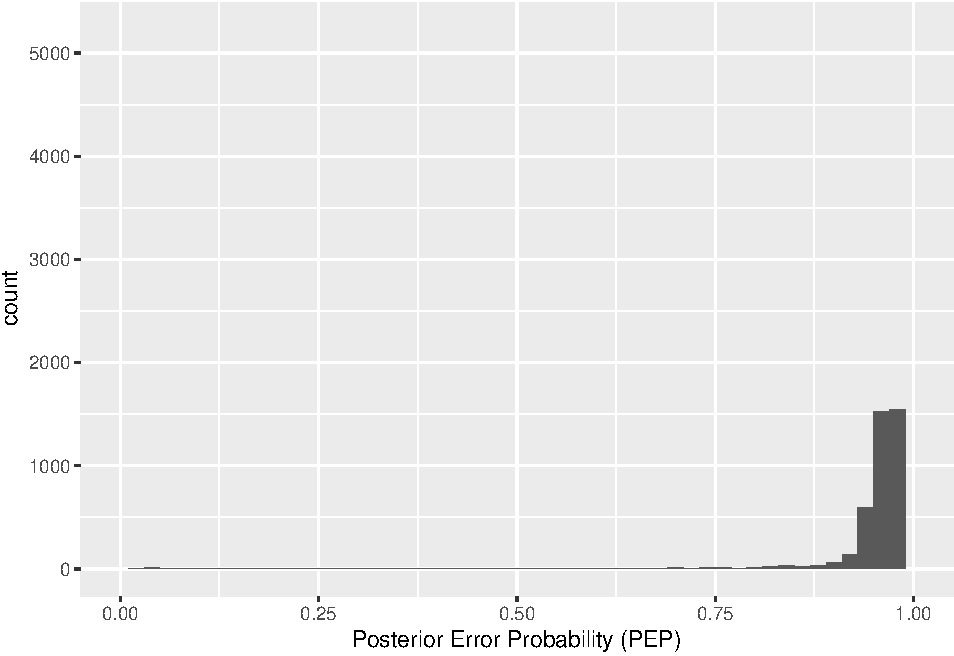
\includegraphics{datadown_files/figure-latex/ap-1.pdf}

\begin{Shaded}
\begin{Highlighting}[]
\CommentTok{# 后验错误率与击球率的关系}
\NormalTok{career_eb }\OperatorTok
\StringTok{    }\KeywordTok{ggplot}\NormalTok{(}\KeywordTok{aes}\NormalTok{(eb_estimate, PEP, }\DataTypeTok{color =}\NormalTok{ AB)) }\OperatorTok{+}
\StringTok{    }\KeywordTok{geom_point}\NormalTok{(}\DataTypeTok{size =} \DecValTok{1}\NormalTok{) }\OperatorTok{+}
\StringTok{    }\KeywordTok{xlab}\NormalTok{(}\StringTok{"(Shrunken) batting average estimate"}\NormalTok{) }\OperatorTok{+}
\StringTok{    }\KeywordTok{ylab}\NormalTok{(}\StringTok{"Posterior Error Probability (PEP)"}\NormalTok{) }\OperatorTok{+}
\StringTok{    }\KeywordTok{geom_vline}\NormalTok{(}\DataTypeTok{color =} \StringTok{"red"}\NormalTok{, }\DataTypeTok{lty =} \DecValTok{2}\NormalTok{, }\DataTypeTok{xintercept =} \FloatTok{.3}\NormalTok{) }\OperatorTok{+}
\StringTok{    }\KeywordTok{scale_colour_gradient}\NormalTok{(}\DataTypeTok{trans =} \StringTok{"log"}\NormalTok{, }\DataTypeTok{breaks =} \DecValTok{10} \OperatorTok{^}\StringTok{ }\NormalTok{(}\DecValTok{1}\OperatorTok{:}\DecValTok{5}\NormalTok{))}
\end{Highlighting}
\end{Shaded}

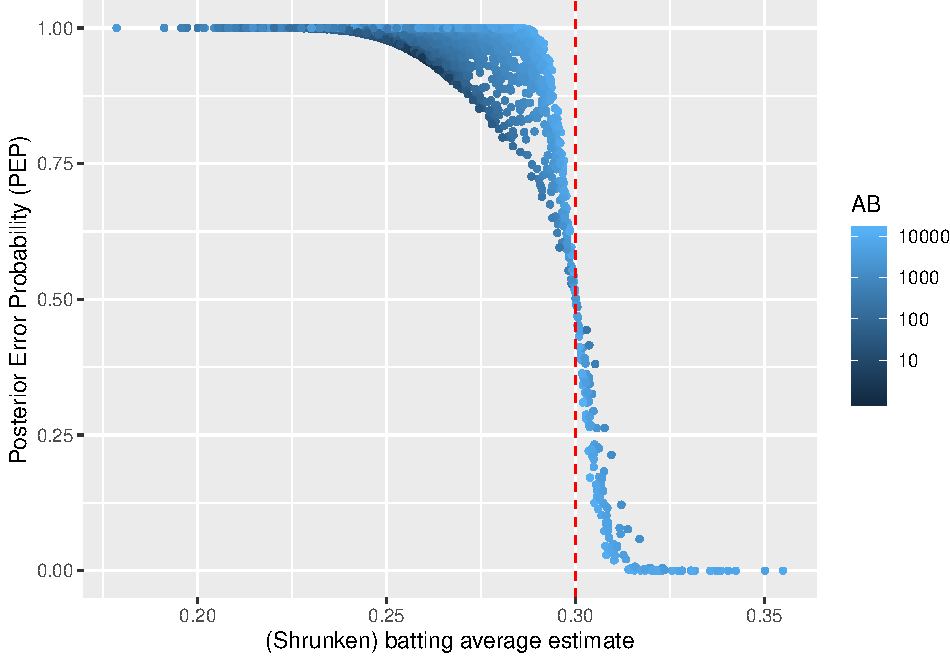
\includegraphics{datadown_files/figure-latex/ap-2.pdf}

\begin{itemize}
\tightlist
\item
  后验错误率高于0.3的多数是击球率与击球数都高的人,因为贝叶斯方法惩罚了击球数低的人
\end{itemize}

\hypertarget{ux9519ux8befux53d1ux73b0ux7387}{%
\section{错误发现率}\label{ux9519ux8befux53d1ux73b0ux7387}}

\begin{itemize}
\item
  错误发现率(FDR)可用来控制一个整体决策,保证整体犯错的概率低于某个数值,错误发现率越高,越可能把假阳性包括进来
\item
  假如我们把进入名人堂的决策作为一个整体,则可允许一定的整体错误率,因为每个人的后验错误率可以计算且期望值线性可加和,我们可以得到一个整体的错误率
\end{itemize}

\begin{Shaded}
\begin{Highlighting}[]
\CommentTok{# 取前100个球员}
\NormalTok{top_players <-}\StringTok{ }\NormalTok{career_eb }\OperatorTok
\StringTok{    }\KeywordTok{arrange}\NormalTok{(PEP) }\OperatorTok
\StringTok{    }\KeywordTok{head}\NormalTok{(}\DecValTok{100}\NormalTok{)}
\CommentTok{# 总错率率}
\KeywordTok{sum}\NormalTok{(top_players}\OperatorTok{$}\NormalTok{PEP)}
\end{Highlighting}
\end{Shaded}

\begin{verbatim}
## [1] 5.17
\end{verbatim}

\begin{Shaded}
\begin{Highlighting}[]
\CommentTok{# 平均错误率}
\KeywordTok{mean}\NormalTok{(top_players}\OperatorTok{$}\NormalTok{PEP)}
\end{Highlighting}
\end{Shaded}

\begin{verbatim}
## [1] 0.0517
\end{verbatim}

\begin{Shaded}
\begin{Highlighting}[]
\CommentTok{# 错误率随所取球员的变化}
\NormalTok{sorted_PEP <-}\StringTok{ }\NormalTok{career_eb }\OperatorTok
\StringTok{    }\KeywordTok{arrange}\NormalTok{(PEP)}

\KeywordTok{mean}\NormalTok{(}\KeywordTok{head}\NormalTok{(sorted_PEP}\OperatorTok{$}\NormalTok{PEP, }\DecValTok{50}\NormalTok{))}
\end{Highlighting}
\end{Shaded}

\begin{verbatim}
## [1] 0.00189
\end{verbatim}

\begin{Shaded}
\begin{Highlighting}[]
\KeywordTok{mean}\NormalTok{(}\KeywordTok{head}\NormalTok{(sorted_PEP}\OperatorTok{$}\NormalTok{PEP, }\DecValTok{200}\NormalTok{))}
\end{Highlighting}
\end{Shaded}

\begin{verbatim}
## [1] 0.25
\end{verbatim}

\begin{itemize}
\tightlist
\item
  错误率在排序后前面低后面高,但这个错误率不特指某个球员,而是包含到某个球员的整体犯错的概率
\end{itemize}

\hypertarget{qux503c}{%
\section{q值}\label{qux503c}}

\begin{itemize}
\tightlist
\item
  q值定义为排序后累积到某个样本的整体平均错误率,类似多重比较中对整体错误率控制的p值
\end{itemize}

\begin{Shaded}
\begin{Highlighting}[]
\CommentTok{# 生成每个球员的q值}
\NormalTok{career_eb <-}\StringTok{ }\NormalTok{career_eb }\OperatorTok
\StringTok{    }\KeywordTok{arrange}\NormalTok{(PEP) }\OperatorTok
\StringTok{    }\KeywordTok{mutate}\NormalTok{(}\DataTypeTok{qvalue =} \KeywordTok{cummean}\NormalTok{(PEP))}
\CommentTok{# 观察不同q值对名人堂球员数的影响}
\NormalTok{career_eb }\OperatorTok
\StringTok{    }\KeywordTok{ggplot}\NormalTok{(}\KeywordTok{aes}\NormalTok{(qvalue, }\KeywordTok{rank}\NormalTok{(PEP))) }\OperatorTok{+}
\StringTok{    }\KeywordTok{geom_line}\NormalTok{() }\OperatorTok{+}
\StringTok{    }\KeywordTok{xlab}\NormalTok{(}\StringTok{"q-value cutoff"}\NormalTok{) }\OperatorTok{+}
\StringTok{    }\KeywordTok{ylab}\NormalTok{(}\StringTok{"Number of players included"}\NormalTok{)}
\end{Highlighting}
\end{Shaded}

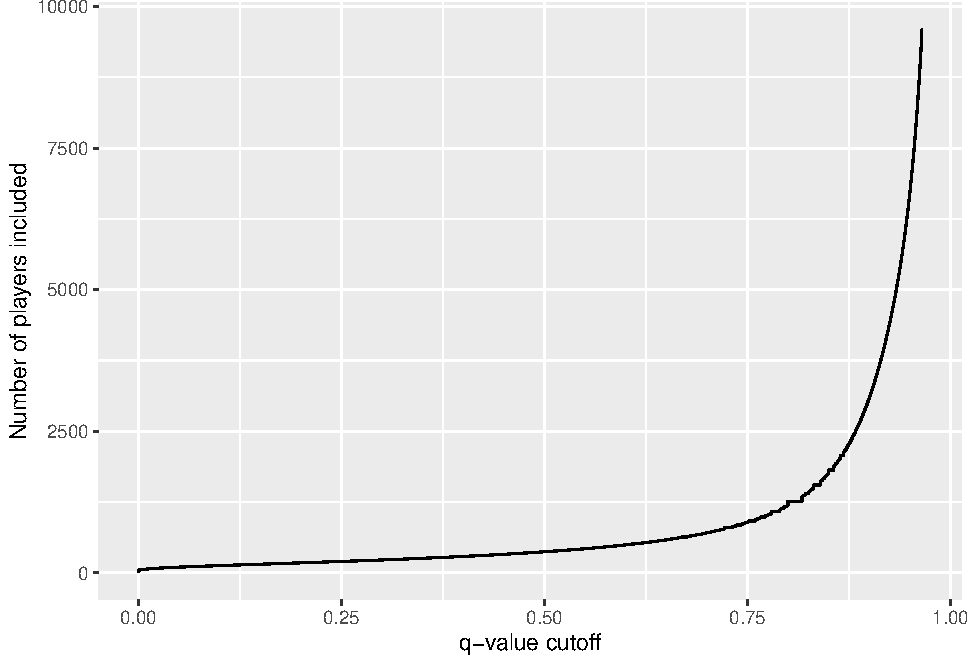
\includegraphics{datadown_files/figure-latex/qvalue-1.pdf}

\begin{Shaded}
\begin{Highlighting}[]
\CommentTok{# 观察小q值部分}
\NormalTok{career_eb }\OperatorTok
\StringTok{    }\KeywordTok{filter}\NormalTok{(qvalue }\OperatorTok{<}\StringTok{ }\FloatTok{.25}\NormalTok{) }\OperatorTok
\StringTok{    }\KeywordTok{ggplot}\NormalTok{(}\KeywordTok{aes}\NormalTok{(qvalue, }\KeywordTok{rank}\NormalTok{(PEP))) }\OperatorTok{+}
\StringTok{    }\KeywordTok{geom_line}\NormalTok{() }\OperatorTok{+}
\StringTok{    }\KeywordTok{xlab}\NormalTok{(}\StringTok{"q-value cutoff"}\NormalTok{) }\OperatorTok{+}
\StringTok{    }\KeywordTok{ylab}\NormalTok{(}\StringTok{"Number of players included"}\NormalTok{)}
\end{Highlighting}
\end{Shaded}

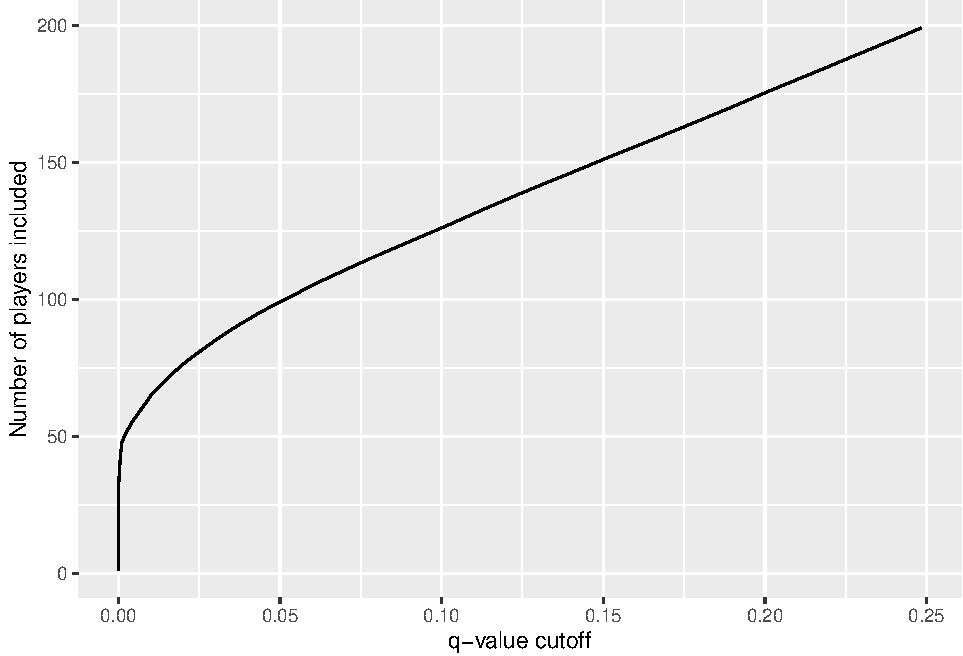
\includegraphics{datadown_files/figure-latex/qvalue-2.pdf}

\begin{itemize}
\item
  200个人进入名人堂可能有约1/4的球员不合适,如果是50个人进入名人堂那么基本不会犯错
\item
  q值是一个整体而非个体的平均错误率,具有累积性,不代表q值大的那一个就是错的
\item
  q值在频率学派的多重比较里也有定义,虽然没有空假设(有先验概率),但实质等同
\end{itemize}

\hypertarget{ux8d1dux53f6ux65afux89c6ux89d2ux7684ux5047ux8bbeux68c0ux9a8c}{%
\section{贝叶斯视角的假设检验}\label{ux8d1dux53f6ux65afux89c6ux89d2ux7684ux5047ux8bbeux68c0ux9a8c}}

\begin{itemize}
\item
  前面描述的是击球率如何求,如何进行区间估计与多个体的错误率控制,面向的个体或整体,那么如何解决比较问题
\item
  设想多个球员,我们考虑如何去比较他们击球率。如果两个球员击球率的概率密度曲线比较接近,那么即便均值有不同我们也无法进行区分;如果重叠比较少,那么我们有理由认为他们之间的差异显著
\item
  贝叶斯视角下如何定量描述这个差异是否显著?
\end{itemize}

\hypertarget{ux6a21ux62dfux9a8cux8bc1}{%
\subsection{模拟验证}\label{ux6a21ux62dfux9a8cux8bc1}}

\begin{itemize}
\tightlist
\item
  单纯取样比大小然后计算比例
\end{itemize}

\begin{Shaded}
\begin{Highlighting}[]
\CommentTok{# 提取两人数据}
\NormalTok{aaron <-}\StringTok{ }\NormalTok{career_eb }\OperatorTok\StringTok{ }\KeywordTok{filter}\NormalTok{(name }\OperatorTok{==}\StringTok{ "Hank Aaron"}\NormalTok{)}
\NormalTok{piazza <-}\StringTok{ }\NormalTok{career_eb }\OperatorTok\StringTok{ }\KeywordTok{filter}\NormalTok{(name }\OperatorTok{==}\StringTok{ "Mike Piazza"}\NormalTok{)}
\CommentTok{# 模拟取样10万次}
\NormalTok{piazza_simulation <-}\StringTok{ }\KeywordTok{rbeta}\NormalTok{(}\FloatTok{1e6}\NormalTok{, piazza}\OperatorTok{$}\NormalTok{alpha1, piazza}\OperatorTok{$}\NormalTok{beta1)}
\NormalTok{aaron_simulation <-}\StringTok{ }\KeywordTok{rbeta}\NormalTok{(}\FloatTok{1e6}\NormalTok{, aaron}\OperatorTok{$}\NormalTok{alpha1, aaron}\OperatorTok{$}\NormalTok{beta1)}
\CommentTok{# 计算一个人超过另一个人的概率}
\NormalTok{sim <-}\StringTok{ }\KeywordTok{mean}\NormalTok{(piazza_simulation }\OperatorTok{>}\StringTok{ }\NormalTok{aaron_simulation)}
\NormalTok{sim}
\end{Highlighting}
\end{Shaded}

\begin{verbatim}
## [1] 0.605
\end{verbatim}

\hypertarget{ux6570ux503cux79efux5206}{%
\subsection{数值积分}\label{ux6570ux503cux79efux5206}}

\begin{itemize}
\tightlist
\item
  两个概率的联合概率分布,然后积分一个队员大于另一个的概率
\end{itemize}

\begin{Shaded}
\begin{Highlighting}[]
\NormalTok{d <-}\StringTok{ }\FloatTok{.00002}
\NormalTok{limits <-}\StringTok{ }\KeywordTok{seq}\NormalTok{(.}\DecValTok{29}\NormalTok{, }\FloatTok{.33}\NormalTok{, d)}
\KeywordTok{sum}\NormalTok{(}\KeywordTok{outer}\NormalTok{(limits, limits, }\ControlFlowTok{function}\NormalTok{(x, y) \{}
\NormalTok{  (x }\OperatorTok{>}\StringTok{ }\NormalTok{y) }\OperatorTok{*}
\StringTok{    }\KeywordTok{dbeta}\NormalTok{(x, piazza}\OperatorTok{$}\NormalTok{alpha1, piazza}\OperatorTok{$}\NormalTok{beta1) }\OperatorTok{*}
\StringTok{    }\KeywordTok{dbeta}\NormalTok{(y, aaron}\OperatorTok{$}\NormalTok{alpha1, aaron}\OperatorTok{$}\NormalTok{beta1) }\OperatorTok{*}
\StringTok{    }\NormalTok{d }\OperatorTok{^}\StringTok{ }\DecValTok{2}
\NormalTok{\}))}
\end{Highlighting}
\end{Shaded}

\begin{verbatim}
## [1] 0.604
\end{verbatim}

\hypertarget{ux89e3ux6790ux89e3}{%
\subsection{解析解}\label{ux89e3ux6790ux89e3}}

\begin{itemize}
\tightlist
\item
  两个贝塔分布一个比另一个高是有含有贝塔函数的解析解的:
\end{itemize}

\[p_A \sim \mbox{Beta}(\alpha_A, \beta_A)\]

\[p_B \sim \mbox{Beta}(\alpha_B, \beta_B)\]

\[{\rm Pr}(p_B > p_A) = \sum_{i=0}^{\alpha_B-1}\frac{B(\alpha_A+i,\beta_A+\beta_B)}{(\beta_B+i) B(1+i, \beta_B) B(\alpha_A, \beta_A) }\]

\begin{Shaded}
\begin{Highlighting}[]
\NormalTok{h <-}\StringTok{ }\ControlFlowTok{function}\NormalTok{(alpha_a, beta_a,}
\NormalTok{              alpha_b, beta_b) \{}
\NormalTok{  j <-}\StringTok{ }\KeywordTok{seq.int}\NormalTok{(}\DecValTok{0}\NormalTok{, }\KeywordTok{round}\NormalTok{(alpha_b) }\OperatorTok{-}\StringTok{ }\DecValTok{1}\NormalTok{)}
\NormalTok{  log_vals <-}\StringTok{ }\NormalTok{(}\KeywordTok{lbeta}\NormalTok{(alpha_a }\OperatorTok{+}\StringTok{ }\NormalTok{j, beta_a }\OperatorTok{+}\StringTok{ }\NormalTok{beta_b) }\OperatorTok{-}\StringTok{ }\KeywordTok{log}\NormalTok{(beta_b }\OperatorTok{+}\StringTok{ }\NormalTok{j) }\OperatorTok{-}
\StringTok{               }\KeywordTok{lbeta}\NormalTok{(}\DecValTok{1} \OperatorTok{+}\StringTok{ }\NormalTok{j, beta_b) }\OperatorTok{-}\StringTok{ }\KeywordTok{lbeta}\NormalTok{(alpha_a, beta_a))}
  \DecValTok{1} \OperatorTok{-}\StringTok{ }\KeywordTok{sum}\NormalTok{(}\KeywordTok{exp}\NormalTok{(log_vals))}
\NormalTok{\}}

\KeywordTok{h}\NormalTok{(piazza}\OperatorTok{$}\NormalTok{alpha1, piazza}\OperatorTok{$}\NormalTok{beta1,}
\NormalTok{  aaron}\OperatorTok{$}\NormalTok{alpha1, aaron}\OperatorTok{$}\NormalTok{beta1)}
\end{Highlighting}
\end{Shaded}

\begin{verbatim}
## [1] 0.603
\end{verbatim}

\hypertarget{ux6b63ux6001ux8fd1ux4f3cux6c42ux89e3}{%
\subsection{正态近似求解}\label{ux6b63ux6001ux8fd1ux4f3cux6c42ux89e3}}

\begin{itemize}
\tightlist
\item
  贝塔分布在\(\alpha\)与\(\beta\)比较大时接近正态分布,可以直接用正态分布的解析解求,速度快很多
\end{itemize}

\begin{Shaded}
\begin{Highlighting}[]
\NormalTok{h_approx <-}\StringTok{ }\ControlFlowTok{function}\NormalTok{(alpha_a, beta_a,}
\NormalTok{                     alpha_b, beta_b) \{}
\NormalTok{  u1 <-}\StringTok{ }\NormalTok{alpha_a }\OperatorTok{/}\StringTok{ }\NormalTok{(alpha_a }\OperatorTok{+}\StringTok{ }\NormalTok{beta_a)}
\NormalTok{  u2 <-}\StringTok{ }\NormalTok{alpha_b }\OperatorTok{/}\StringTok{ }\NormalTok{(alpha_b }\OperatorTok{+}\StringTok{ }\NormalTok{beta_b)}
\NormalTok{  var1 <-}\StringTok{ }\NormalTok{alpha_a }\OperatorTok{*}\StringTok{ }\NormalTok{beta_a }\OperatorTok{/}\StringTok{ }\NormalTok{((alpha_a }\OperatorTok{+}\StringTok{ }\NormalTok{beta_a) }\OperatorTok{^}\StringTok{ }\DecValTok{2} \OperatorTok{*}\StringTok{ }\NormalTok{(alpha_a }\OperatorTok{+}\StringTok{ }\NormalTok{beta_a }\OperatorTok{+}\StringTok{ }\DecValTok{1}\NormalTok{))}
\NormalTok{  var2 <-}\StringTok{ }\NormalTok{alpha_b }\OperatorTok{*}\StringTok{ }\NormalTok{beta_b }\OperatorTok{/}\StringTok{ }\NormalTok{((alpha_b }\OperatorTok{+}\StringTok{ }\NormalTok{beta_b) }\OperatorTok{^}\StringTok{ }\DecValTok{2} \OperatorTok{*}\StringTok{ }\NormalTok{(alpha_b }\OperatorTok{+}\StringTok{ }\NormalTok{beta_b }\OperatorTok{+}\StringTok{ }\DecValTok{1}\NormalTok{))}
  \KeywordTok{pnorm}\NormalTok{(}\DecValTok{0}\NormalTok{, u2 }\OperatorTok{-}\StringTok{ }\NormalTok{u1, }\KeywordTok{sqrt}\NormalTok{(var1 }\OperatorTok{+}\StringTok{ }\NormalTok{var2))}
\NormalTok{\}}

\KeywordTok{h_approx}\NormalTok{(piazza}\OperatorTok{$}\NormalTok{alpha1, piazza}\OperatorTok{$}\NormalTok{beta1, aaron}\OperatorTok{$}\NormalTok{alpha1, aaron}\OperatorTok{$}\NormalTok{beta1)}
\end{Highlighting}
\end{Shaded}

\begin{verbatim}
## [1] 0.605
\end{verbatim}

\hypertarget{ux6bd4ux4f8bux68c0ux9a8c}{%
\section{比例检验}\label{ux6bd4ux4f8bux68c0ux9a8c}}

\begin{itemize}
\tightlist
\item
  这是个列联表问题,频率学派对比两个比例
\end{itemize}

\begin{Shaded}
\begin{Highlighting}[]
\NormalTok{two_players <-}\StringTok{ }\KeywordTok{bind_rows}\NormalTok{(aaron, piazza)}

\NormalTok{two_players }\OperatorTok
\StringTok{  }\KeywordTok{transmute}\NormalTok{(}\DataTypeTok{Player =}\NormalTok{ name, }\DataTypeTok{Hits =}\NormalTok{ H, }\DataTypeTok{Misses =}\NormalTok{ AB }\OperatorTok{-}\StringTok{ }\NormalTok{H) }\OperatorTok
\StringTok{  }\NormalTok{knitr}\OperatorTok{::}\KeywordTok{kable}\NormalTok{()}
\end{Highlighting}
\end{Shaded}

\begin{tabular}{l|r|r}
\hline
Player & Hits & Misses\\
\hline
Hank Aaron & 3771 & 8593\\
\hline
Mike Piazza & 2127 & 4784\\
\hline
\end{tabular}

\begin{Shaded}
\begin{Highlighting}[]
\KeywordTok{prop.test}\NormalTok{(two_players}\OperatorTok{$}\NormalTok{H, two_players}\OperatorTok{$}\NormalTok{AB)}
\end{Highlighting}
\end{Shaded}

\begin{verbatim}
## 
##  2-sample test for equality of proportions with continuity
##  correction
## 
## data:  two_players$H out of two_players$AB
## X-squared = 0.1, df = 1, p-value = 0.7
## alternative hypothesis: two.sided
## 95 percent confidence interval:
##  -0.0165  0.0109
## sample estimates:
## prop 1 prop 2 
##  0.305  0.308
\end{verbatim}

\begin{itemize}
\tightlist
\item
  贝叶斯学派对比两个比例
\end{itemize}

\begin{Shaded}
\begin{Highlighting}[]
\NormalTok{credible_interval_approx <-}\StringTok{ }\ControlFlowTok{function}\NormalTok{(a, b, c, d) \{}
\NormalTok{  u1 <-}\StringTok{ }\NormalTok{a }\OperatorTok{/}\StringTok{ }\NormalTok{(a }\OperatorTok{+}\StringTok{ }\NormalTok{b)}
\NormalTok{  u2 <-}\StringTok{ }\NormalTok{c }\OperatorTok{/}\StringTok{ }\NormalTok{(c }\OperatorTok{+}\StringTok{ }\NormalTok{d)}
\NormalTok{  var1 <-}\StringTok{ }\NormalTok{a }\OperatorTok{*}\StringTok{ }\NormalTok{b }\OperatorTok{/}\StringTok{ }\NormalTok{((a }\OperatorTok{+}\StringTok{ }\NormalTok{b) }\OperatorTok{^}\StringTok{ }\DecValTok{2} \OperatorTok{*}\StringTok{ }\NormalTok{(a }\OperatorTok{+}\StringTok{ }\NormalTok{b }\OperatorTok{+}\StringTok{ }\DecValTok{1}\NormalTok{))}
\NormalTok{  var2 <-}\StringTok{ }\NormalTok{c }\OperatorTok{*}\StringTok{ }\NormalTok{d }\OperatorTok{/}\StringTok{ }\NormalTok{((c }\OperatorTok{+}\StringTok{ }\NormalTok{d) }\OperatorTok{^}\StringTok{ }\DecValTok{2} \OperatorTok{*}\StringTok{ }\NormalTok{(c }\OperatorTok{+}\StringTok{ }\NormalTok{d }\OperatorTok{+}\StringTok{ }\DecValTok{1}\NormalTok{))}

\NormalTok{  mu_diff <-}\StringTok{ }\NormalTok{u2 }\OperatorTok{-}\StringTok{ }\NormalTok{u1}
\NormalTok{  sd_diff <-}\StringTok{ }\KeywordTok{sqrt}\NormalTok{(var1 }\OperatorTok{+}\StringTok{ }\NormalTok{var2)}

  \KeywordTok{data_frame}\NormalTok{(}\DataTypeTok{posterior =} \KeywordTok{pnorm}\NormalTok{(}\DecValTok{0}\NormalTok{, mu_diff, sd_diff),}
             \DataTypeTok{estimate =}\NormalTok{ mu_diff,}
             \DataTypeTok{conf.low =} \KeywordTok{qnorm}\NormalTok{(.}\DecValTok{025}\NormalTok{, mu_diff, sd_diff),}
             \DataTypeTok{conf.high =} \KeywordTok{qnorm}\NormalTok{(.}\DecValTok{975}\NormalTok{, mu_diff, sd_diff))}
\NormalTok{\}}

\KeywordTok{credible_interval_approx}\NormalTok{(piazza}\OperatorTok{$}\NormalTok{alpha1, piazza}\OperatorTok{$}\NormalTok{beta1, aaron}\OperatorTok{$}\NormalTok{alpha1, aaron}\OperatorTok{$}\NormalTok{beta1)}
\end{Highlighting}
\end{Shaded}

\begin{verbatim}
## # A tibble: 1 x 4
##   posterior estimate conf.low conf.high
##       <dbl>    <dbl>    <dbl>     <dbl>
## 1     0.605 -0.00181  -0.0151    0.0115
\end{verbatim}

\begin{itemize}
\tightlist
\item
  多个球员对比一个
\end{itemize}

\begin{Shaded}
\begin{Highlighting}[]
\KeywordTok{set.seed}\NormalTok{(}\DecValTok{2016}\NormalTok{)}

\NormalTok{intervals <-}\StringTok{ }\NormalTok{career_eb }\OperatorTok
\StringTok{  }\KeywordTok{filter}\NormalTok{(AB }\OperatorTok{>}\StringTok{ }\DecValTok{10}\NormalTok{) }\OperatorTok
\StringTok{  }\KeywordTok{sample_n}\NormalTok{(}\DecValTok{20}\NormalTok{) }\OperatorTok
\StringTok{  }\KeywordTok{group_by}\NormalTok{(name, H, AB) }\OperatorTok
\StringTok{  }\KeywordTok{do}\NormalTok{(}\KeywordTok{credible_interval_approx}\NormalTok{(piazza}\OperatorTok{$}\NormalTok{alpha1, piazza}\OperatorTok{$}\NormalTok{beta1, .}\OperatorTok{$}\NormalTok{alpha1, .}\OperatorTok{$}\NormalTok{beta1)) }\OperatorTok
\StringTok{  }\KeywordTok{ungroup}\NormalTok{() }\OperatorTok
\StringTok{  }\KeywordTok{mutate}\NormalTok{(}\DataTypeTok{name =} \KeywordTok{reorder}\NormalTok{(}\KeywordTok{paste0}\NormalTok{(name, }\StringTok{" ("}\NormalTok{, H, }\StringTok{" / "}\NormalTok{, AB, }\StringTok{")"}\NormalTok{), }\OperatorTok{-}\NormalTok{estimate))}
\NormalTok{f <-}\StringTok{ }\ControlFlowTok{function}\NormalTok{(H, AB) broom}\OperatorTok{::}\KeywordTok{tidy}\NormalTok{(}\KeywordTok{prop.test}\NormalTok{(}\KeywordTok{c}\NormalTok{(H, piazza}\OperatorTok{$}\NormalTok{H), }\KeywordTok{c}\NormalTok{(AB, piazza}\OperatorTok{$}\NormalTok{AB)))}
\NormalTok{prop_tests <-}\StringTok{ }\NormalTok{purrr}\OperatorTok{::}\KeywordTok{map2_df}\NormalTok{(intervals}\OperatorTok{$}\NormalTok{H, intervals}\OperatorTok{$}\NormalTok{AB, f) }\OperatorTok
\StringTok{  }\KeywordTok{mutate}\NormalTok{(}\DataTypeTok{estimate =}\NormalTok{ estimate1 }\OperatorTok{-}\StringTok{ }\NormalTok{estimate2,}
         \DataTypeTok{name =}\NormalTok{ intervals}\OperatorTok{$}\NormalTok{name)}

\NormalTok{all_intervals <-}\StringTok{ }\KeywordTok{bind_rows}\NormalTok{(}
  \KeywordTok{mutate}\NormalTok{(intervals, }\DataTypeTok{type =} \StringTok{"Credible"}\NormalTok{),}
  \KeywordTok{mutate}\NormalTok{(prop_tests, }\DataTypeTok{type =} \StringTok{"Confidence"}\NormalTok{)}
\NormalTok{)}

\KeywordTok{ggplot}\NormalTok{(all_intervals, }\KeywordTok{aes}\NormalTok{(}\DataTypeTok{x =}\NormalTok{ estimate, }\DataTypeTok{y =}\NormalTok{ name, }\DataTypeTok{color =}\NormalTok{ type)) }\OperatorTok{+}
\StringTok{  }\KeywordTok{geom_point}\NormalTok{() }\OperatorTok{+}
\StringTok{  }\KeywordTok{geom_errorbarh}\NormalTok{(}\KeywordTok{aes}\NormalTok{(}\DataTypeTok{xmin =}\NormalTok{ conf.low, }\DataTypeTok{xmax =}\NormalTok{ conf.high)) }\OperatorTok{+}
\StringTok{  }\KeywordTok{xlab}\NormalTok{(}\StringTok{"Piazza average - player average"}\NormalTok{) }\OperatorTok{+}
\StringTok{  }\KeywordTok{ylab}\NormalTok{(}\StringTok{"Player"}\NormalTok{)}
\end{Highlighting}
\end{Shaded}

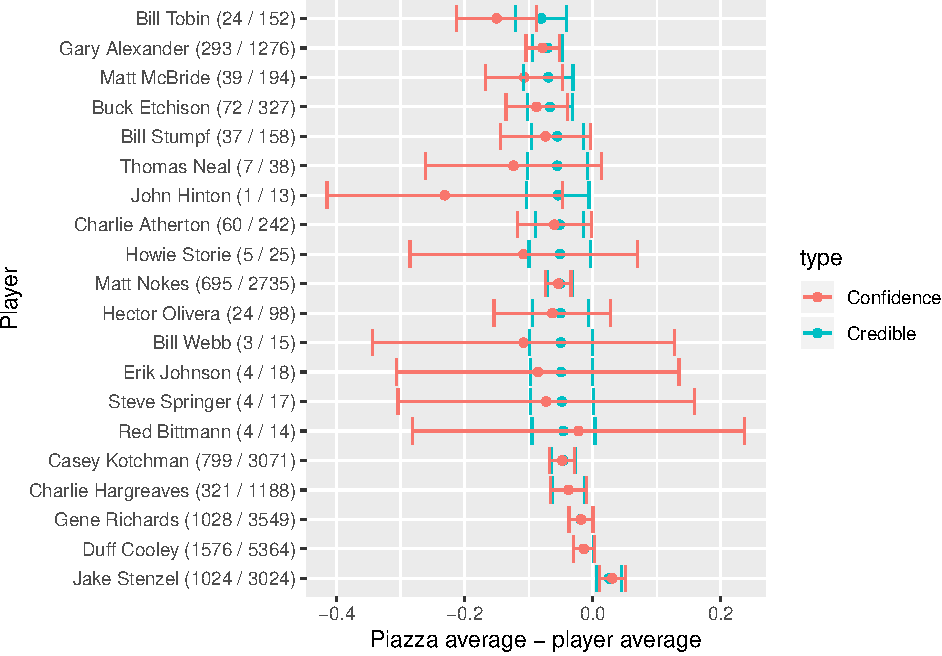
\includegraphics{datadown_files/figure-latex/mp-1.pdf}

\begin{itemize}
\tightlist
\item
  置信区间与可信区间的主要差异来自于经验贝叶斯的区间收敛
\end{itemize}

\hypertarget{ux9519ux8befux7387ux63a7ux5236}{%
\section{错误率控制}\label{ux9519ux8befux7387ux63a7ux5236}}

\begin{itemize}
\item
  如果我打算交易一个球员,那么如何筛选候选人?
\item
  先选那些击球率更好的球员
\end{itemize}

\begin{Shaded}
\begin{Highlighting}[]
\CommentTok{# 对比打算交易的球员与其他球员}
\NormalTok{career_eb_vs_piazza <-}\StringTok{ }\KeywordTok{bind_cols}\NormalTok{(}
\NormalTok{  career_eb,}
  \KeywordTok{credible_interval_approx}\NormalTok{(piazza}\OperatorTok{$}\NormalTok{alpha1, piazza}\OperatorTok{$}\NormalTok{beta1,}
\NormalTok{                           career_eb}\OperatorTok{$}\NormalTok{alpha1, career_eb}\OperatorTok{$}\NormalTok{beta1)) }\OperatorTok
\StringTok{  }\NormalTok{dplyr}\OperatorTok{::}\KeywordTok{select}\NormalTok{(name, posterior, conf.low, conf.high)}

\NormalTok{career_eb_vs_piazza}
\end{Highlighting}
\end{Shaded}

\begin{verbatim}
## # A tibble: 9,670 x 4
##    name                 posterior conf.low conf.high
##    <chr>                    <dbl>    <dbl>     <dbl>
##  1 Rogers Hornsby        2.84e-11   0.0345    0.0639
##  2 Ed Delahanty          7.52e- 7   0.0217    0.0517
##  3 Shoeless Joe Jackson  8.89e- 8   0.0278    0.0611
##  4 Willie Keeler         4.62e- 6   0.0183    0.0472
##  5 Nap Lajoie            1.55e- 5   0.0159    0.0441
##  6 Tony Gwynn            1.83e- 5   0.0157    0.0442
##  7 Harry Heilmann        7.19e- 6   0.0180    0.0476
##  8 Lou Gehrig            1.43e- 5   0.0167    0.0461
##  9 Billy Hamilton        6.47e- 6   0.0191    0.0504
## 10 Eddie Collins         1.99e- 4   0.0113    0.0393
## # ... with 9,660 more rows
\end{verbatim}

\begin{Shaded}
\begin{Highlighting}[]
\CommentTok{# 计算q值}
\NormalTok{career_eb_vs_piazza <-}\StringTok{ }\NormalTok{career_eb_vs_piazza }\OperatorTok
\StringTok{  }\KeywordTok{arrange}\NormalTok{(posterior) }\OperatorTok
\StringTok{  }\KeywordTok{mutate}\NormalTok{(}\DataTypeTok{qvalue =} \KeywordTok{cummean}\NormalTok{(posterior))}

\CommentTok{# 筛选那些q值小于0.05的}
\NormalTok{better <-}\StringTok{ }\NormalTok{career_eb_vs_piazza }\OperatorTok
\StringTok{  }\KeywordTok{filter}\NormalTok{(qvalue }\OperatorTok{<}\StringTok{ }\FloatTok{.05}\NormalTok{)}

\NormalTok{better}
\end{Highlighting}
\end{Shaded}

\begin{verbatim}
## # A tibble: 48 x 5
##    name                 posterior conf.low conf.high   qvalue
##    <chr>                    <dbl>    <dbl>     <dbl>    <dbl>
##  1 Rogers Hornsby        2.84e-11   0.0345    0.0639 2.84e-11
##  2 Shoeless Joe Jackson  8.89e- 8   0.0278    0.0611 4.45e- 8
##  3 Ed Delahanty          7.52e- 7   0.0217    0.0517 2.80e- 7
##  4 Willie Keeler         4.62e- 6   0.0183    0.0472 1.36e- 6
##  5 Billy Hamilton        6.47e- 6   0.0191    0.0504 2.39e- 6
##  6 Harry Heilmann        7.19e- 6   0.0180    0.0476 3.19e- 6
##  7 Lou Gehrig            1.43e- 5   0.0167    0.0461 4.78e- 6
##  8 Nap Lajoie            1.55e- 5   0.0159    0.0441 6.12e- 6
##  9 Tony Gwynn            1.83e- 5   0.0157    0.0442 7.47e- 6
## 10 Bill Terry            3.04e- 5   0.0162    0.0472 9.77e- 6
## # ... with 38 more rows
\end{verbatim}

\begin{itemize}
\tightlist
\item
  这样我们筛到一个可交易的群体,总和错误率不超过5\%
\end{itemize}

\hypertarget{ux5f71ux54cdux56e0ux5b50}{%
\section{影响因子}\label{ux5f71ux54cdux56e0ux5b50}}

\begin{itemize}
\tightlist
\item
  击球率高除了能力影响外还有可能是因为得到的机会多或者光环效应,例如一开始凭运气打得好,后面给机会多,通过经验累积提高了击球率
\end{itemize}

\begin{Shaded}
\begin{Highlighting}[]
\NormalTok{career }\OperatorTok
\StringTok{  }\KeywordTok{filter}\NormalTok{(AB }\OperatorTok{>=}\StringTok{ }\DecValTok{20}\NormalTok{) }\OperatorTok
\StringTok{  }\KeywordTok{ggplot}\NormalTok{(}\KeywordTok{aes}\NormalTok{(AB, average)) }\OperatorTok{+}
\StringTok{  }\KeywordTok{geom_point}\NormalTok{() }\OperatorTok{+}
\StringTok{  }\KeywordTok{geom_smooth}\NormalTok{(}\DataTypeTok{method =} \StringTok{"lm"}\NormalTok{, }\DataTypeTok{se =} \OtherTok{FALSE}\NormalTok{) }\OperatorTok{+}
\StringTok{  }\KeywordTok{scale_x_log10}\NormalTok{()}
\end{Highlighting}
\end{Shaded}

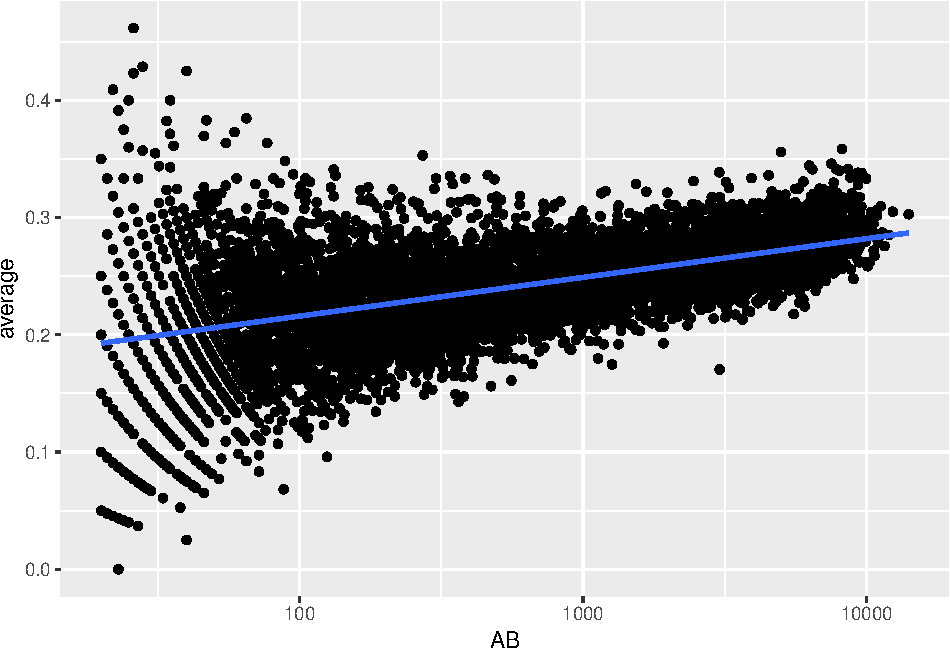
\includegraphics{datadown_files/figure-latex/if-1.pdf}

\begin{itemize}
\item
  击球数低方差会大,这比较正常,很多人挂在起跑线上了
\item
  直接使用经验贝叶斯方法会导致整体向均值收敛,这高估了新手的数据
\end{itemize}

\begin{Shaded}
\begin{Highlighting}[]
\NormalTok{prior_mu <-}\StringTok{ }\NormalTok{alpha0 }\OperatorTok{/}\StringTok{ }\NormalTok{(alpha0 }\OperatorTok{+}\StringTok{ }\NormalTok{beta0)}
\NormalTok{career_eb }\OperatorTok
\StringTok{  }\KeywordTok{filter}\NormalTok{(AB }\OperatorTok{>=}\StringTok{ }\DecValTok{20}\NormalTok{) }\OperatorTok
\StringTok{  }\KeywordTok{gather}\NormalTok{(type, value, average, eb_estimate) }\OperatorTok
\StringTok{  }\KeywordTok{mutate}\NormalTok{(}\DataTypeTok{type =}\NormalTok{ plyr}\OperatorTok{::}\KeywordTok{revalue}\NormalTok{(type, }\KeywordTok{c}\NormalTok{(}\DataTypeTok{average =} \StringTok{"Raw"}\NormalTok{,}
                                      \DataTypeTok{eb_estimate =} \StringTok{"With EB Shrinkage"}\NormalTok{))) }\OperatorTok
\StringTok{  }\KeywordTok{ggplot}\NormalTok{(}\KeywordTok{aes}\NormalTok{(AB, value)) }\OperatorTok{+}
\StringTok{  }\KeywordTok{geom_point}\NormalTok{() }\OperatorTok{+}
\StringTok{  }\KeywordTok{scale_x_log10}\NormalTok{() }\OperatorTok{+}
\StringTok{  }\KeywordTok{geom_hline}\NormalTok{(}\DataTypeTok{color =} \StringTok{"red"}\NormalTok{, }\DataTypeTok{lty =} \DecValTok{2}\NormalTok{, }\DataTypeTok{size =} \FloatTok{1.5}\NormalTok{, }\DataTypeTok{yintercept =}\NormalTok{ prior_mu) }\OperatorTok{+}
\StringTok{  }\KeywordTok{facet_wrap}\NormalTok{(}\OperatorTok{~}\NormalTok{type) }\OperatorTok{+}
\StringTok{  }\KeywordTok{ylab}\NormalTok{(}\StringTok{"average"}\NormalTok{) }\OperatorTok{+}
\StringTok{    }\KeywordTok{geom_smooth}\NormalTok{(}\DataTypeTok{method =} \StringTok{"lm"}\NormalTok{)}
\end{Highlighting}
\end{Shaded}

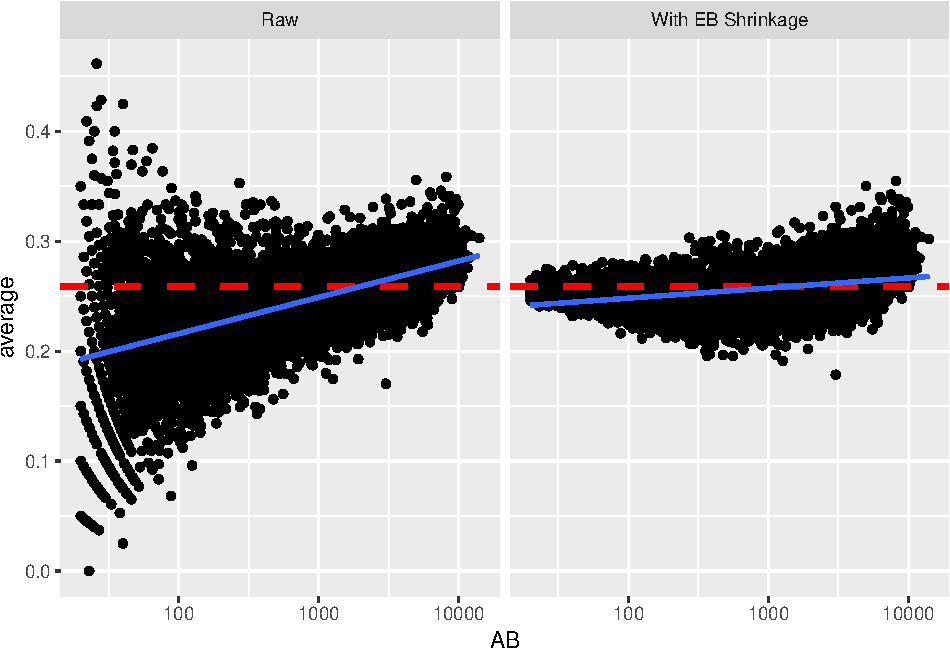
\includegraphics{datadown_files/figure-latex/ife-1.pdf}

\begin{itemize}
\item
  为了如实反应这种情况,我们应该认为击球率符合贝塔分布,但同时贝塔分布的两个参数受击球数的影响,击球数越多,越可能击中
\item
  这个模型可以用贝塔-二项式回归来描述
\end{itemize}

\[\mu_i = \mu_0 + \mu_{\mbox{AB}} \cdot \log(\mbox{AB})\]

\[\alpha_{0,i} = \mu_i / \sigma_0\]

\[\beta_{0,i} = (1 - \mu_i) / \sigma_0\]

\[p_i \sim \mbox{Beta}(\alpha_{0,i}, \beta_{0,i})\]

\[H_i \sim \mbox{Binom}(\mbox{AB}_i, p_i)\]

\hypertarget{ux62dfux5408ux6a21ux578b}{%
\subsection{拟合模型}\label{ux62dfux5408ux6a21ux578b}}

\begin{itemize}
\tightlist
\item
  寻找拟合后的模型参数,构建新的先验概率
\end{itemize}

\begin{Shaded}
\begin{Highlighting}[]
\KeywordTok{library}\NormalTok{(gamlss)}
\CommentTok{# 拟合模型}
\NormalTok{fit <-}\StringTok{ }\KeywordTok{gamlss}\NormalTok{(}\KeywordTok{cbind}\NormalTok{(H, AB }\OperatorTok{-}\StringTok{ }\NormalTok{H) }\OperatorTok{~}\StringTok{ }\KeywordTok{log}\NormalTok{(AB),}
              \DataTypeTok{data =}\NormalTok{ career_eb,}
              \DataTypeTok{family =} \KeywordTok{BB}\NormalTok{(}\DataTypeTok{mu.link =} \StringTok{"identity"}\NormalTok{))}
\end{Highlighting}
\end{Shaded}

\begin{verbatim}
## GAMLSS-RS iteration 1: Global Deviance = 94587 
## GAMLSS-RS iteration 2: Global Deviance = 74795 
## GAMLSS-RS iteration 3: Global Deviance = 70515 
## GAMLSS-RS iteration 4: Global Deviance = 70509 
## GAMLSS-RS iteration 5: Global Deviance = 70509
\end{verbatim}

\begin{Shaded}
\begin{Highlighting}[]
\CommentTok{# 展示拟合参数}
\NormalTok{td <-}\StringTok{ }\KeywordTok{tidy}\NormalTok{(fit)}
\NormalTok{td}
\end{Highlighting}
\end{Shaded}

\begin{verbatim}
## # A tibble: 3 x 6
##   parameter term        estimate std.error statistic p.value
##   <chr>     <chr>          <dbl>     <dbl>     <dbl>   <dbl>
## 1 mu        (Intercept)   0.144   0.00158       91.0       0
## 2 mu        log(AB)       0.0151  0.000216      70.0       0
## 3 sigma     (Intercept)  -6.35    0.0246      -258.        0
\end{verbatim}

\begin{Shaded}
\begin{Highlighting}[]
\CommentTok{# 构建新的先验概率}
\NormalTok{mu_}\DecValTok{0}\NormalTok{ <-}\StringTok{ }\NormalTok{td}\OperatorTok{$}\NormalTok{estimate[}\DecValTok{1}\NormalTok{]}
\NormalTok{mu_AB <-}\StringTok{ }\NormalTok{td}\OperatorTok{$}\NormalTok{estimate[}\DecValTok{2}\NormalTok{]}
\NormalTok{sigma <-}\StringTok{ }\KeywordTok{exp}\NormalTok{(td}\OperatorTok{$}\NormalTok{estimate[}\DecValTok{3}\NormalTok{])}

\CommentTok{# 看看AB对先验概率的影响}
\KeywordTok{crossing}\NormalTok{(}\DataTypeTok{x =} \KeywordTok{seq}\NormalTok{(}\FloatTok{0.08}\NormalTok{, }\FloatTok{.35}\NormalTok{, }\FloatTok{.001}\NormalTok{), }\DataTypeTok{AB =} \KeywordTok{c}\NormalTok{(}\DecValTok{1}\NormalTok{, }\DecValTok{10}\NormalTok{, }\DecValTok{100}\NormalTok{, }\DecValTok{1000}\NormalTok{, }\DecValTok{10000}\NormalTok{)) }\OperatorTok
\StringTok{  }\KeywordTok{mutate}\NormalTok{(}\DataTypeTok{density =} \KeywordTok{dbeta}\NormalTok{(x, (mu_}\DecValTok{0} \OperatorTok{+}\StringTok{ }\NormalTok{mu_AB }\OperatorTok{*}\StringTok{ }\KeywordTok{log}\NormalTok{(AB)) }\OperatorTok{/}\StringTok{ }\NormalTok{sigma,}
\NormalTok{                         (}\DecValTok{1} \OperatorTok{-}\StringTok{ }\NormalTok{(mu_}\DecValTok{0} \OperatorTok{+}\StringTok{ }\NormalTok{mu_AB }\OperatorTok{*}\StringTok{ }\KeywordTok{log}\NormalTok{(AB))) }\OperatorTok{/}\StringTok{ }\NormalTok{sigma)) }\OperatorTok
\StringTok{  }\KeywordTok{mutate}\NormalTok{(}\DataTypeTok{AB =} \KeywordTok{factor}\NormalTok{(AB)) }\OperatorTok
\StringTok{  }\KeywordTok{ggplot}\NormalTok{(}\KeywordTok{aes}\NormalTok{(x, density, }\DataTypeTok{color =}\NormalTok{ AB, }\DataTypeTok{group =}\NormalTok{ AB)) }\OperatorTok{+}
\StringTok{  }\KeywordTok{geom_line}\NormalTok{() }\OperatorTok{+}
\StringTok{  }\KeywordTok{xlab}\NormalTok{(}\StringTok{"Batting average"}\NormalTok{) }\OperatorTok{+}
\StringTok{  }\KeywordTok{ylab}\NormalTok{(}\StringTok{"Prior density"}\NormalTok{)}
\end{Highlighting}
\end{Shaded}

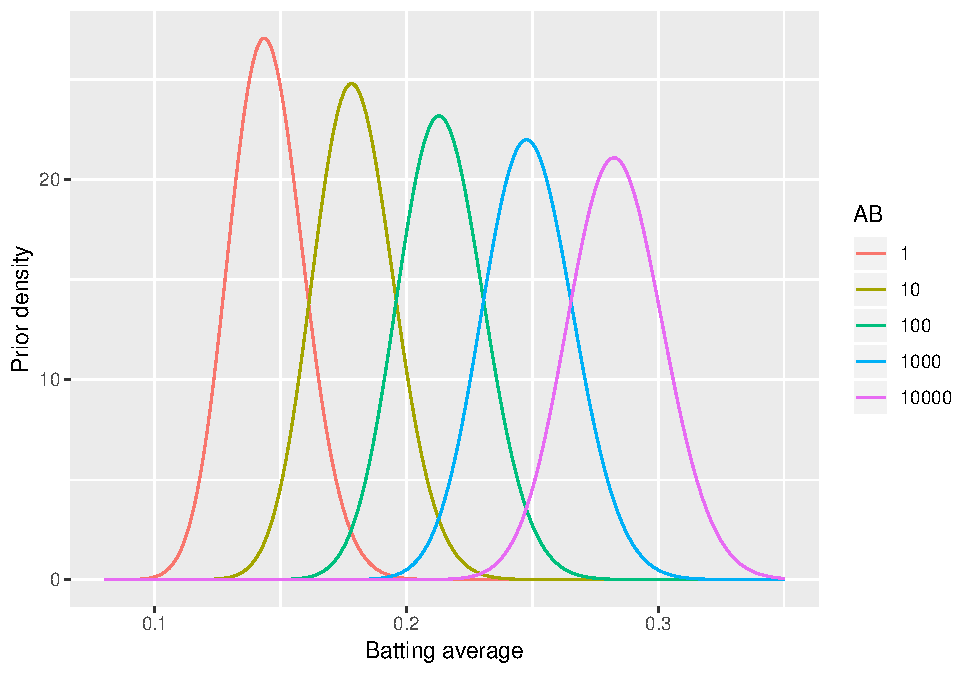
\includegraphics{datadown_files/figure-latex/fitbb-1.pdf}

\hypertarget{ux6c42ux540eux9a8cux6982ux7387}{%
\subsection{求后验概率}\label{ux6c42ux540eux9a8cux6982ux7387}}

\begin{Shaded}
\begin{Highlighting}[]
\CommentTok{# 计算所有拟合值}
\NormalTok{mu <-}\StringTok{ }\KeywordTok{fitted}\NormalTok{(fit, }\DataTypeTok{parameter =} \StringTok{"mu"}\NormalTok{)}
\NormalTok{sigma <-}\StringTok{ }\KeywordTok{fitted}\NormalTok{(fit, }\DataTypeTok{parameter =} \StringTok{"sigma"}\NormalTok{)}
\CommentTok{# 计算所有后验概率}
\NormalTok{career_eb_wAB <-}\StringTok{ }\NormalTok{career_eb }\OperatorTok
\StringTok{  }\NormalTok{dplyr}\OperatorTok{::}\KeywordTok{select}\NormalTok{(name, H, AB, }\DataTypeTok{original_eb =}\NormalTok{ eb_estimate) }\OperatorTok
\StringTok{  }\KeywordTok{mutate}\NormalTok{(}\DataTypeTok{mu =}\NormalTok{ mu,}
         \DataTypeTok{alpha0 =}\NormalTok{ mu }\OperatorTok{/}\StringTok{ }\NormalTok{sigma,}
         \DataTypeTok{beta0 =}\NormalTok{ (}\DecValTok{1} \OperatorTok{-}\StringTok{ }\NormalTok{mu) }\OperatorTok{/}\StringTok{ }\NormalTok{sigma,}
         \DataTypeTok{alpha1 =}\NormalTok{ alpha0 }\OperatorTok{+}\StringTok{ }\NormalTok{H,}
         \DataTypeTok{beta1 =}\NormalTok{ beta0 }\OperatorTok{+}\StringTok{ }\NormalTok{AB }\OperatorTok{-}\StringTok{ }\NormalTok{H,}
         \DataTypeTok{new_eb =}\NormalTok{ alpha1 }\OperatorTok{/}\StringTok{ }\NormalTok{(alpha1 }\OperatorTok{+}\StringTok{ }\NormalTok{beta1))}
\CommentTok{# 展示拟合后的击球率}
\KeywordTok{ggplot}\NormalTok{(career_eb_wAB, }\KeywordTok{aes}\NormalTok{(original_eb, new_eb, }\DataTypeTok{color =}\NormalTok{ AB)) }\OperatorTok{+}
\StringTok{  }\KeywordTok{geom_point}\NormalTok{() }\OperatorTok{+}
\StringTok{  }\KeywordTok{geom_abline}\NormalTok{(}\DataTypeTok{color =} \StringTok{"red"}\NormalTok{) }\OperatorTok{+}
\StringTok{  }\KeywordTok{xlab}\NormalTok{(}\StringTok{"Original EB Estimate"}\NormalTok{) }\OperatorTok{+}
\StringTok{  }\KeywordTok{ylab}\NormalTok{(}\StringTok{"EB Estimate w/ AB term"}\NormalTok{) }\OperatorTok{+}
\StringTok{  }\KeywordTok{scale_color_continuous}\NormalTok{(}\DataTypeTok{trans =} \StringTok{"log"}\NormalTok{, }\DataTypeTok{breaks =} \DecValTok{10} \OperatorTok{^}\StringTok{ }\NormalTok{(}\DecValTok{0}\OperatorTok{:}\DecValTok{4}\NormalTok{))}
\end{Highlighting}
\end{Shaded}

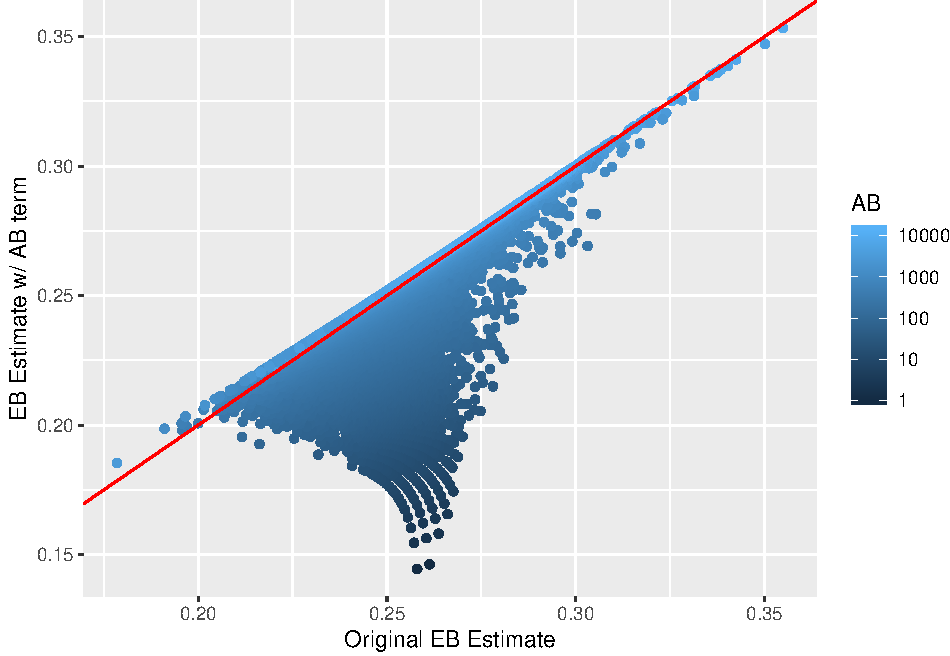
\includegraphics{datadown_files/figure-latex/fitpo-1.pdf}

\begin{Shaded}
\begin{Highlighting}[]
\CommentTok{# 对比}
\KeywordTok{library}\NormalTok{(tidyr)}

\NormalTok{lev <-}\StringTok{ }\KeywordTok{c}\NormalTok{(}\DataTypeTok{raw =} \StringTok{"Raw H / AB"}\NormalTok{, }\DataTypeTok{original_eb =} \StringTok{"EB Estimate"}\NormalTok{, }\DataTypeTok{new_eb =} \StringTok{"EB w/ Regression"}\NormalTok{)}

\NormalTok{career_eb_wAB }\OperatorTok
\StringTok{  }\KeywordTok{filter}\NormalTok{(AB }\OperatorTok{>=}\StringTok{ }\DecValTok{10}\NormalTok{) }\OperatorTok
\StringTok{  }\KeywordTok{mutate}\NormalTok{(}\DataTypeTok{raw =}\NormalTok{ H }\OperatorTok{/}\StringTok{ }\NormalTok{AB) }\OperatorTok
\StringTok{  }\KeywordTok{gather}\NormalTok{(type, value, raw, original_eb, new_eb) }\OperatorTok
\StringTok{  }\KeywordTok{mutate}\NormalTok{(}\DataTypeTok{mu =} \KeywordTok{ifelse}\NormalTok{(type }\OperatorTok{==}\StringTok{ "original_eb"}\NormalTok{, prior_mu,}
                     \KeywordTok{ifelse}\NormalTok{(type }\OperatorTok{==}\StringTok{ "new_eb"}\NormalTok{, mu, }\OtherTok{NA}\NormalTok{))) }\OperatorTok
\StringTok{  }\KeywordTok{mutate}\NormalTok{(}\DataTypeTok{type =} \KeywordTok{factor}\NormalTok{(plyr}\OperatorTok{::}\KeywordTok{revalue}\NormalTok{(type, lev), lev)) }\OperatorTok
\StringTok{  }\KeywordTok{ggplot}\NormalTok{(}\KeywordTok{aes}\NormalTok{(AB, value)) }\OperatorTok{+}
\StringTok{  }\KeywordTok{geom_point}\NormalTok{() }\OperatorTok{+}
\StringTok{  }\KeywordTok{geom_line}\NormalTok{(}\KeywordTok{aes}\NormalTok{(}\DataTypeTok{y =}\NormalTok{ mu), }\DataTypeTok{color =} \StringTok{"red"}\NormalTok{) }\OperatorTok{+}
\StringTok{  }\KeywordTok{scale_x_log10}\NormalTok{() }\OperatorTok{+}
\StringTok{  }\KeywordTok{facet_wrap}\NormalTok{(}\OperatorTok{~}\NormalTok{type) }\OperatorTok{+}
\StringTok{  }\KeywordTok{xlab}\NormalTok{(}\StringTok{"At-Bats (AB)"}\NormalTok{) }\OperatorTok{+}
\StringTok{  }\KeywordTok{ylab}\NormalTok{(}\StringTok{"Estimate"}\NormalTok{)}
\end{Highlighting}
\end{Shaded}

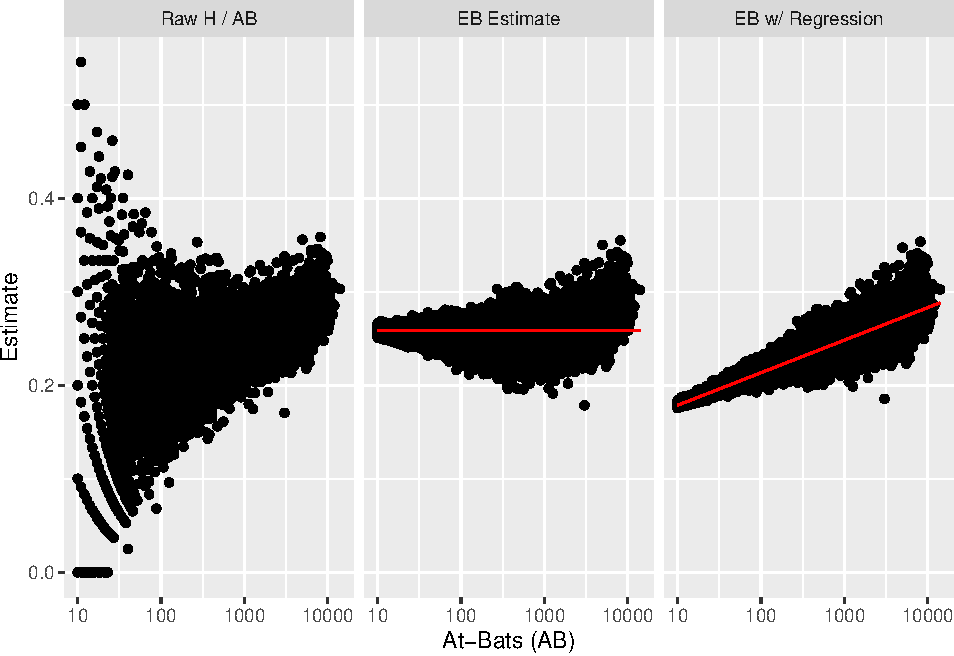
\includegraphics{datadown_files/figure-latex/fitpo-2.pdf}

\begin{itemize}
\tightlist
\item
  矫正后我们的数据更复合现实了,其实这是贝叶斯分层模型的一个简单版本,通过考虑更多因素,我们可以构建更复杂的模型来挖掘出我们所需要的信息
\end{itemize}

\hypertarget{ux8003ux8651ux66f4ux591aux56e0ux7d20}{%
\subsection{考虑更多因素}\label{ux8003ux8651ux66f4ux591aux56e0ux7d20}}

\begin{itemize}
\tightlist
\item
  现在我们听说左利手跟右利手的表现可能不一样,所以我们要对模型进行完善,考虑把左右手参数加入模型
\end{itemize}

\begin{Shaded}
\begin{Highlighting}[]
\CommentTok{# 展示数据}
\NormalTok{career2 }\OperatorTok
\StringTok{        }\KeywordTok{count}\NormalTok{(bats)}
\end{Highlighting}
\end{Shaded}

\begin{verbatim}
## # A tibble: 4 x 2
##   bats      n
##   <fct> <int>
## 1 B       788
## 2 L      2740
## 3 R      5486
## 4 <NA>    656
\end{verbatim}

\begin{Shaded}
\begin{Highlighting}[]
\CommentTok{# 排除NA}
\NormalTok{career3 <-}\StringTok{ }\NormalTok{career2 }\OperatorTok
\StringTok{  }\KeywordTok{filter}\NormalTok{(}\OperatorTok{!}\KeywordTok{is.na}\NormalTok{(bats)) }\OperatorTok
\StringTok{  }\KeywordTok{mutate}\NormalTok{(}\DataTypeTok{bats =} \KeywordTok{relevel}\NormalTok{(bats, }\StringTok{"R"}\NormalTok{))}
\CommentTok{# 重建模型}
\NormalTok{fit2 <-}\StringTok{ }\KeywordTok{gamlss}\NormalTok{(}\KeywordTok{cbind}\NormalTok{(H, AB }\OperatorTok{-}\StringTok{ }\NormalTok{H) }\OperatorTok{~}\StringTok{ }\KeywordTok{log}\NormalTok{(AB) }\OperatorTok{+}\StringTok{ }\NormalTok{bats,}
               \DataTypeTok{data =}\NormalTok{ career3,}
               \DataTypeTok{family =} \KeywordTok{BB}\NormalTok{(}\DataTypeTok{mu.link =} \StringTok{"identity"}\NormalTok{))}
\end{Highlighting}
\end{Shaded}

\begin{verbatim}
## GAMLSS-RS iteration 1: Global Deviance = 90843 
## GAMLSS-RS iteration 2: Global Deviance = 71587 
## GAMLSS-RS iteration 3: Global Deviance = 67295 
## GAMLSS-RS iteration 4: Global Deviance = 67289 
## GAMLSS-RS iteration 5: Global Deviance = 67289
\end{verbatim}

\begin{Shaded}
\begin{Highlighting}[]
\CommentTok{# 观察参数}
\KeywordTok{tidy}\NormalTok{(fit2)}
\end{Highlighting}
\end{Shaded}

\begin{verbatim}
## # A tibble: 5 x 6
##   parameter term        estimate std.error statistic  p.value
##   <chr>     <chr>          <dbl>     <dbl>     <dbl>    <dbl>
## 1 mu        (Intercept)  0.142    0.00162      87.6  0.      
## 2 mu        log(AB)      0.0150   0.000219     68.3  0.      
## 3 mu        batsB       -0.00158  0.000982     -1.61 1.07e- 1
## 4 mu        batsL        0.00953  0.000630     15.1  5.11e-51
## 5 sigma     (Intercept) -6.43     0.0251     -256.   0.
\end{verbatim}

\begin{Shaded}
\begin{Highlighting}[]
\NormalTok{sigma <-}\StringTok{ }\KeywordTok{fitted}\NormalTok{(fit2, }\StringTok{"sigma"}\NormalTok{)[}\DecValTok{1}\NormalTok{]}
\KeywordTok{crossing}\NormalTok{(}\DataTypeTok{bats =} \KeywordTok{c}\NormalTok{(}\StringTok{"L"}\NormalTok{, }\StringTok{"R"}\NormalTok{),}
         \DataTypeTok{AB =} \KeywordTok{c}\NormalTok{(}\DecValTok{1}\NormalTok{, }\DecValTok{10}\NormalTok{, }\DecValTok{100}\NormalTok{, }\DecValTok{1000}\NormalTok{, }\DecValTok{10000}\NormalTok{)) }\OperatorTok
\StringTok{  }\KeywordTok{augment}\NormalTok{(fit2, }\DataTypeTok{newdata =}\NormalTok{ .) }\OperatorTok
\StringTok{  }\KeywordTok{rename}\NormalTok{(}\DataTypeTok{mu =}\NormalTok{ .fitted) }\OperatorTok
\StringTok{  }\KeywordTok{crossing}\NormalTok{(}\DataTypeTok{x =} \KeywordTok{seq}\NormalTok{(.}\DecValTok{1}\NormalTok{, }\FloatTok{.36}\NormalTok{, }\FloatTok{.0005}\NormalTok{)) }\OperatorTok
\StringTok{  }\KeywordTok{mutate}\NormalTok{(}\DataTypeTok{alpha =}\NormalTok{ mu }\OperatorTok{/}\StringTok{ }\NormalTok{sigma,}
         \DataTypeTok{beta =}\NormalTok{ (}\DecValTok{1} \OperatorTok{-}\StringTok{ }\NormalTok{mu) }\OperatorTok{/}\StringTok{ }\NormalTok{sigma,}
         \DataTypeTok{density =} \KeywordTok{dbeta}\NormalTok{(x, alpha, beta)) }\OperatorTok
\StringTok{  }\KeywordTok{ggplot}\NormalTok{(}\KeywordTok{aes}\NormalTok{(x, density, }\DataTypeTok{color =} \KeywordTok{factor}\NormalTok{(AB), }\DataTypeTok{lty =}\NormalTok{ bats)) }\OperatorTok{+}
\StringTok{  }\KeywordTok{geom_line}\NormalTok{() }\OperatorTok{+}
\StringTok{  }\KeywordTok{labs}\NormalTok{(}\DataTypeTok{x =} \StringTok{"Batting average"}\NormalTok{,}
       \DataTypeTok{y =} \StringTok{"Prior density"}\NormalTok{,}
       \DataTypeTok{color =} \StringTok{"AB"}\NormalTok{,}
       \DataTypeTok{lty =} \StringTok{"Batting hand"}\NormalTok{)}
\end{Highlighting}
\end{Shaded}

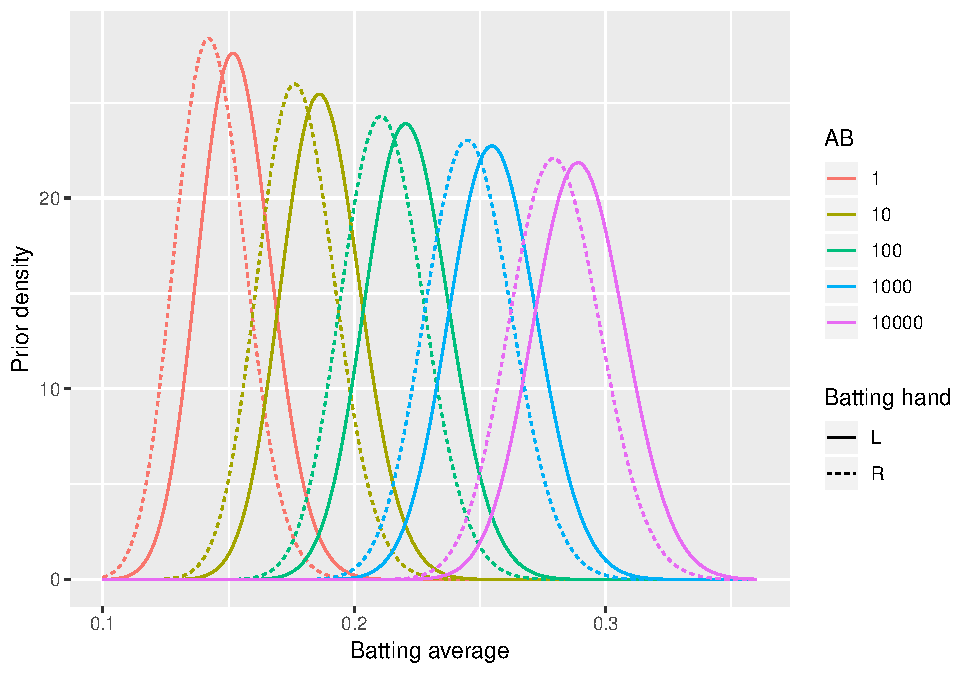
\includegraphics{datadown_files/figure-latex/career2-1.pdf}

\begin{itemize}
\tightlist
\item
  存在先验概率的情况下,可以考虑考察随着击球数增长左右手的不同
\end{itemize}

\begin{Shaded}
\begin{Highlighting}[]
\KeywordTok{crossing}\NormalTok{(}\DataTypeTok{bats =} \KeywordTok{c}\NormalTok{(}\StringTok{"L"}\NormalTok{, }\StringTok{"R"}\NormalTok{),}
         \DataTypeTok{AB =} \KeywordTok{c}\NormalTok{(}\DecValTok{10}\NormalTok{, }\DecValTok{100}\NormalTok{, }\DecValTok{1000}\NormalTok{, }\DecValTok{10000}\NormalTok{)) }\OperatorTok
\StringTok{  }\KeywordTok{augment}\NormalTok{(fit2, }\DataTypeTok{newdata =}\NormalTok{ .) }\OperatorTok
\StringTok{  }\KeywordTok{mutate}\NormalTok{(}\DataTypeTok{H =} \FloatTok{.3} \OperatorTok{*}\StringTok{ }\NormalTok{AB,}
         \DataTypeTok{alpha0 =}\NormalTok{ .fitted }\OperatorTok{/}\StringTok{ }\NormalTok{sigma,}
         \DataTypeTok{beta0 =}\NormalTok{ (}\DecValTok{1} \OperatorTok{-}\StringTok{ }\NormalTok{.fitted) }\OperatorTok{/}\StringTok{ }\NormalTok{sigma,}
         \DataTypeTok{alpha1 =}\NormalTok{ alpha0 }\OperatorTok{+}\StringTok{ }\NormalTok{H,}
         \DataTypeTok{beta1 =}\NormalTok{ beta0 }\OperatorTok{+}\StringTok{ }\NormalTok{AB }\OperatorTok{-}\StringTok{ }\NormalTok{H,}
         \DataTypeTok{estimate =}\NormalTok{ alpha1 }\OperatorTok{/}\StringTok{ }\NormalTok{(alpha1 }\OperatorTok{+}\StringTok{ }\NormalTok{beta1),}
         \DataTypeTok{conf.low =} \KeywordTok{qbeta}\NormalTok{(.}\DecValTok{025}\NormalTok{, alpha1, beta1),}
         \DataTypeTok{conf.high =} \KeywordTok{qbeta}\NormalTok{(.}\DecValTok{975}\NormalTok{, alpha1, beta1),}
         \DataTypeTok{record =} \KeywordTok{paste}\NormalTok{(H, AB, }\DataTypeTok{sep =} \StringTok{" / "}\NormalTok{)) }\OperatorTok
\StringTok{  }\KeywordTok{ggplot}\NormalTok{(}\KeywordTok{aes}\NormalTok{(estimate, record, }\DataTypeTok{color =}\NormalTok{ bats)) }\OperatorTok{+}
\StringTok{  }\KeywordTok{geom_point}\NormalTok{() }\OperatorTok{+}
\StringTok{  }\KeywordTok{geom_errorbarh}\NormalTok{(}\KeywordTok{aes}\NormalTok{(}\DataTypeTok{xmin =}\NormalTok{ conf.low, }\DataTypeTok{xmax =}\NormalTok{ conf.high)) }\OperatorTok{+}
\StringTok{  }\KeywordTok{labs}\NormalTok{(}\DataTypeTok{x =} \StringTok{"Estimate w/ 95% credible interval"}\NormalTok{,}
       \DataTypeTok{y =} \StringTok{"Batting record"}\NormalTok{,}
       \DataTypeTok{color =} \StringTok{"Batting hand"}\NormalTok{)}
\end{Highlighting}
\end{Shaded}

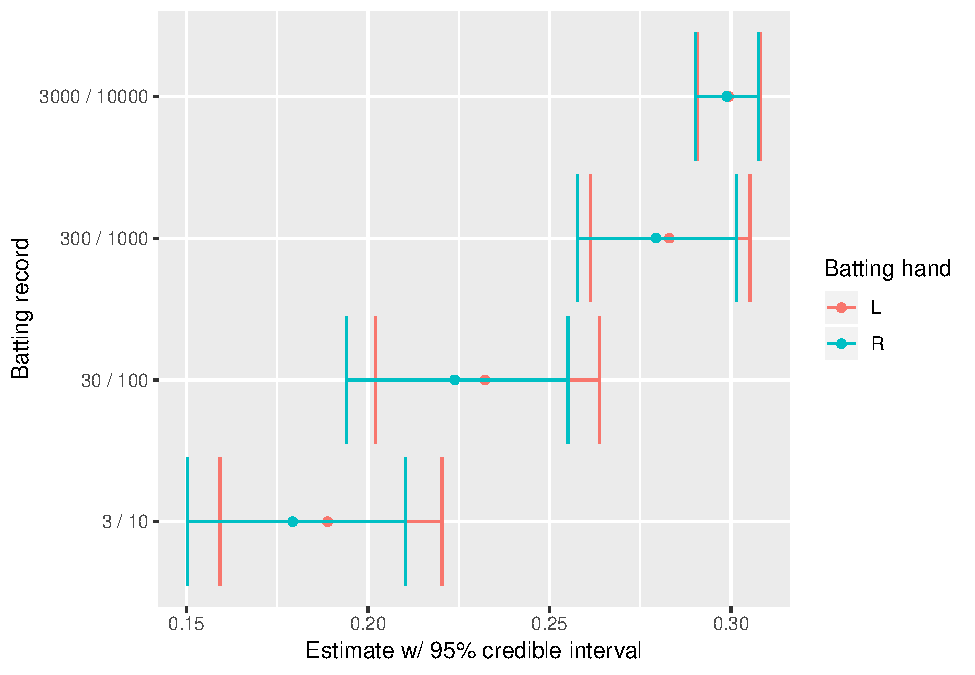
\includegraphics{datadown_files/figure-latex/lrcom-1.pdf}

\begin{itemize}
\tightlist
\item
  另一个要考虑的因素是不同年份的平均击球率可能也有起伏
\end{itemize}

\begin{Shaded}
\begin{Highlighting}[]
\NormalTok{career3 }\OperatorTok
\StringTok{  }\KeywordTok{mutate}\NormalTok{(}\DataTypeTok{decade =} \KeywordTok{factor}\NormalTok{(}\KeywordTok{round}\NormalTok{(year }\OperatorTok{-}\StringTok{ }\DecValTok{5}\NormalTok{, }\DecValTok{-1}\NormalTok{))) }\OperatorTok
\StringTok{  }\KeywordTok{filter}\NormalTok{(AB }\OperatorTok{>=}\StringTok{ }\DecValTok{500}\NormalTok{) }\OperatorTok
\StringTok{  }\KeywordTok{ggplot}\NormalTok{(}\KeywordTok{aes}\NormalTok{(decade, average)) }\OperatorTok{+}
\StringTok{  }\KeywordTok{geom_boxplot}\NormalTok{() }\OperatorTok{+}
\StringTok{  }\KeywordTok{theme}\NormalTok{(}\DataTypeTok{axis.text.x =} \KeywordTok{element_text}\NormalTok{(}\DataTypeTok{angle =} \DecValTok{90}\NormalTok{, }\DataTypeTok{hjust =} \DecValTok{1}\NormalTok{)) }\OperatorTok{+}
\StringTok{  }\KeywordTok{ylab}\NormalTok{(}\StringTok{"Batting average"}\NormalTok{)}
\CommentTok{# 用样条插值来进行拟合}
\KeywordTok{library}\NormalTok{(splines)}
\NormalTok{fit3 <-}\StringTok{ }\KeywordTok{gamlss}\NormalTok{(}\KeywordTok{cbind}\NormalTok{(H, AB }\OperatorTok{-}\StringTok{ }\NormalTok{H) }\OperatorTok{~}\StringTok{ }\DecValTok{0} \OperatorTok{+}\StringTok{ }\KeywordTok{ns}\NormalTok{(year, }\DataTypeTok{df =} \DecValTok{5}\NormalTok{) }\OperatorTok{+}\StringTok{ }\NormalTok{bats }\OperatorTok{+}\StringTok{ }\KeywordTok{log}\NormalTok{(AB),}
               \DataTypeTok{data =}\NormalTok{ career3,}
               \DataTypeTok{family =} \KeywordTok{BB}\NormalTok{(}\DataTypeTok{mu.link =} \StringTok{"identity"}\NormalTok{))}

\CommentTok{# 观察在击球数1000上先验概率的变化}
\NormalTok{plot_gamlss_fit <-}\StringTok{ }\ControlFlowTok{function}\NormalTok{(f) \{}
\NormalTok{  career3 }\OperatorTok
\StringTok{    }\NormalTok{dplyr}\OperatorTok{::}\KeywordTok{select}\NormalTok{(year, bats) }\OperatorTok
\StringTok{    }\KeywordTok{distinct}\NormalTok{() }\OperatorTok
\StringTok{    }\KeywordTok{filter}\NormalTok{(bats }\OperatorTok{!=}\StringTok{ "B"}\NormalTok{) }\OperatorTok
\StringTok{    }\KeywordTok{mutate}\NormalTok{(}\DataTypeTok{AB =} \DecValTok{1000}\NormalTok{) }\OperatorTok
\StringTok{    }\KeywordTok{augment}\NormalTok{(f, }\DataTypeTok{newdata =}\NormalTok{ .) }\OperatorTok
\StringTok{    }\KeywordTok{rename}\NormalTok{(}\DataTypeTok{mu =}\NormalTok{ .fitted) }\OperatorTok
\StringTok{    }\KeywordTok{mutate}\NormalTok{(}\DataTypeTok{sigma =} \KeywordTok{fitted}\NormalTok{(fit3, }\StringTok{"sigma"}\NormalTok{)[}\DecValTok{1}\NormalTok{],}
           \DataTypeTok{alpha0 =}\NormalTok{ mu }\OperatorTok{/}\StringTok{ }\NormalTok{sigma,}
           \DataTypeTok{beta0 =}\NormalTok{ (}\DecValTok{1} \OperatorTok{-}\StringTok{ }\NormalTok{mu) }\OperatorTok{/}\StringTok{ }\NormalTok{sigma,}
           \DataTypeTok{conf_low =} \KeywordTok{qbeta}\NormalTok{(.}\DecValTok{025}\NormalTok{, alpha0, beta0),}
           \DataTypeTok{conf_high =} \KeywordTok{qbeta}\NormalTok{(.}\DecValTok{975}\NormalTok{, alpha0, beta0)) }\OperatorTok
\StringTok{    }\KeywordTok{ggplot}\NormalTok{(}\KeywordTok{aes}\NormalTok{(year, mu, }\DataTypeTok{color =}\NormalTok{ bats, }\DataTypeTok{group =}\NormalTok{ bats)) }\OperatorTok{+}
\StringTok{    }\KeywordTok{geom_line}\NormalTok{() }\OperatorTok{+}
\StringTok{    }\KeywordTok{geom_ribbon}\NormalTok{(}\KeywordTok{aes}\NormalTok{(}\DataTypeTok{ymin =}\NormalTok{ conf_low, }\DataTypeTok{ymax =}\NormalTok{ conf_high), }\DataTypeTok{linetype =} \DecValTok{2}\NormalTok{, }\DataTypeTok{alpha =} \FloatTok{.1}\NormalTok{) }\OperatorTok{+}
\StringTok{    }\KeywordTok{labs}\NormalTok{(}\DataTypeTok{x =} \StringTok{"Year"}\NormalTok{,}
         \DataTypeTok{y =} \StringTok{"Prior distribution (median + 95% quantiles)"}\NormalTok{,}
         \DataTypeTok{color =} \StringTok{"Batting hand"}\NormalTok{)}
\NormalTok{\}}
\KeywordTok{plot_gamlss_fit}\NormalTok{(fit3)}
\end{Highlighting}
\end{Shaded}

\begin{itemize}
\tightlist
\item
  同时另一个问题是这些因素会交互影响
\end{itemize}

\begin{Shaded}
\begin{Highlighting}[]
\NormalTok{fit4 <-}\StringTok{ }\KeywordTok{gamlss}\NormalTok{(}\KeywordTok{cbind}\NormalTok{(H, AB }\OperatorTok{-}\StringTok{ }\NormalTok{H) }\OperatorTok{~}\StringTok{ }\DecValTok{0} \OperatorTok{+}\StringTok{ }\KeywordTok{ns}\NormalTok{(year, }\DecValTok{5}\NormalTok{) }\OperatorTok{*}\StringTok{ }\NormalTok{bats }\OperatorTok{+}\StringTok{ }\KeywordTok{log}\NormalTok{(AB),}
               \DataTypeTok{data =}\NormalTok{ career3,}
               \DataTypeTok{family =} \KeywordTok{BB}\NormalTok{(}\DataTypeTok{mu.link =} \StringTok{"identity"}\NormalTok{))}
\KeywordTok{plot_gamlss_fit}\NormalTok{(fit4)}

\NormalTok{Pitching }\OperatorTok
\StringTok{  }\NormalTok{dplyr}\OperatorTok{::}\KeywordTok{select}\NormalTok{(playerID, yearID, GS) }\OperatorTok
\StringTok{  }\KeywordTok{distinct}\NormalTok{() }\OperatorTok
\StringTok{  }\KeywordTok{inner_join}\NormalTok{(dplyr}\OperatorTok{::}\KeywordTok{select}\NormalTok{(Master, playerID, throws)) }\OperatorTok
\StringTok{  }\KeywordTok{count}\NormalTok{(yearID, throws, }\DataTypeTok{wt =}\NormalTok{ GS) }\OperatorTok
\StringTok{  }\KeywordTok{filter}\NormalTok{(}\OperatorTok{!}\KeywordTok{is.na}\NormalTok{(throws)) }\OperatorTok
\StringTok{  }\KeywordTok{mutate}\NormalTok{(}\DataTypeTok{percent =}\NormalTok{ n }\OperatorTok{/}\StringTok{ }\KeywordTok{sum}\NormalTok{(n)) }\OperatorTok
\StringTok{  }\KeywordTok{filter}\NormalTok{(throws }\OperatorTok{==}\StringTok{ "L"}\NormalTok{) }\OperatorTok
\StringTok{  }\KeywordTok{ggplot}\NormalTok{(}\KeywordTok{aes}\NormalTok{(yearID, percent)) }\OperatorTok{+}
\StringTok{  }\KeywordTok{geom_line}\NormalTok{() }\OperatorTok{+}
\StringTok{  }\KeywordTok{geom_smooth}\NormalTok{() }\OperatorTok{+}
\StringTok{  }\KeywordTok{scale_y_continuous}\NormalTok{(}\DataTypeTok{labels =}\NormalTok{ scales}\OperatorTok{::}\KeywordTok{percent_format}\NormalTok{()) }\OperatorTok{+}
\StringTok{  }\KeywordTok{xlab}\NormalTok{(}\StringTok{"Year"}\NormalTok{) }\OperatorTok{+}
\StringTok{  }\KeywordTok{ylab}\NormalTok{(}\StringTok{"% of games with left-handed pitcher"}\NormalTok{)}
\end{Highlighting}
\end{Shaded}

\begin{itemize}
\tightlist
\item
  左右手之间的差距伴随年份在逐渐减少
\end{itemize}

\begin{Shaded}
\begin{Highlighting}[]
\NormalTok{players <-}\StringTok{ }\KeywordTok{crossing}\NormalTok{(}\DataTypeTok{year =} \KeywordTok{c}\NormalTok{(}\DecValTok{1915}\NormalTok{, }\DecValTok{1965}\NormalTok{, }\DecValTok{2015}\NormalTok{),}
                    \DataTypeTok{bats =} \KeywordTok{c}\NormalTok{(}\StringTok{"L"}\NormalTok{, }\StringTok{"R"}\NormalTok{),}
                    \DataTypeTok{H =} \DecValTok{30}\NormalTok{,}
                    \DataTypeTok{AB =} \DecValTok{100}\NormalTok{)}

\NormalTok{players_posterior <-}\StringTok{ }\NormalTok{players }\OperatorTok
\StringTok{  }\KeywordTok{mutate}\NormalTok{(}\DataTypeTok{mu =} \KeywordTok{predict}\NormalTok{(fit4, }\DataTypeTok{what =} \StringTok{"mu"}\NormalTok{, }\DataTypeTok{newdata =}\NormalTok{ players),}
         \DataTypeTok{sigma =} \KeywordTok{predict}\NormalTok{(fit4, }\DataTypeTok{what =} \StringTok{"sigma"}\NormalTok{, }\DataTypeTok{newdata =}\NormalTok{ players, }\DataTypeTok{type =} \StringTok{"response"}\NormalTok{),}
         \DataTypeTok{alpha0 =}\NormalTok{ mu }\OperatorTok{/}\StringTok{ }\NormalTok{sigma,}
         \DataTypeTok{beta0 =}\NormalTok{ (}\DecValTok{1} \OperatorTok{-}\StringTok{ }\NormalTok{mu) }\OperatorTok{/}\StringTok{ }\NormalTok{sigma,}
         \DataTypeTok{alpha1 =}\NormalTok{ alpha0 }\OperatorTok{+}\StringTok{ }\NormalTok{H,}
         \DataTypeTok{beta1 =}\NormalTok{ beta0 }\OperatorTok{+}\StringTok{ }\NormalTok{AB }\OperatorTok{-}\StringTok{ }\NormalTok{H)}
\NormalTok{players_posterior }\OperatorTok
\StringTok{  }\KeywordTok{crossing}\NormalTok{(}\DataTypeTok{x =} \KeywordTok{seq}\NormalTok{(.}\DecValTok{15}\NormalTok{, }\FloatTok{.3}\NormalTok{, }\FloatTok{.001}\NormalTok{)) }\OperatorTok
\StringTok{  }\KeywordTok{mutate}\NormalTok{(}\DataTypeTok{density =} \KeywordTok{dbeta}\NormalTok{(x, alpha1, beta1)) }\OperatorTok
\StringTok{  }\KeywordTok{ggplot}\NormalTok{(}\KeywordTok{aes}\NormalTok{(x, density, }\DataTypeTok{color =}\NormalTok{ bats)) }\OperatorTok{+}
\StringTok{  }\KeywordTok{geom_line}\NormalTok{() }\OperatorTok{+}
\StringTok{  }\KeywordTok{facet_wrap}\NormalTok{(}\OperatorTok{~}\StringTok{ }\NormalTok{year) }\OperatorTok{+}
\StringTok{  }\KeywordTok{xlab}\NormalTok{(}\StringTok{"Batting average"}\NormalTok{) }\OperatorTok{+}
\StringTok{  }\KeywordTok{ylab}\NormalTok{(}\StringTok{"Posterior density"}\NormalTok{) }\OperatorTok{+}
\StringTok{  }\KeywordTok{ggtitle}\NormalTok{(}\StringTok{"Posterior distributions for batters with 30 / 100"}\NormalTok{)}
\end{Highlighting}
\end{Shaded}

\begin{itemize}
\tightlist
\item
  经验贝叶斯对先验概率的估计类似频率学派,但进行的又是贝叶斯分析
\end{itemize}

\hypertarget{ux6df7ux5408ux6982ux7387ux6a21ux578b}{%
\section{混合概率模型}\label{ux6df7ux5408ux6982ux7387ux6a21ux578b}}

\begin{itemize}
\tightlist
\item
  用击球概率为例,击球手跟非击球手的概率分布是不一样的,那么实际看到的总体球员概率分布应该是一个混合在一起的两个独立分布
\end{itemize}

\begin{Shaded}
\begin{Highlighting}[]
\CommentTok{# 找出投球3次以上的人}
\NormalTok{pitchers <-}\StringTok{ }\NormalTok{Pitching }\OperatorTok
\StringTok{  }\KeywordTok{group_by}\NormalTok{(playerID) }\OperatorTok
\StringTok{  }\KeywordTok{summarize}\NormalTok{(}\DataTypeTok{gamesPitched =} \KeywordTok{sum}\NormalTok{(G)) }\OperatorTok
\StringTok{  }\KeywordTok{filter}\NormalTok{(gamesPitched }\OperatorTok{>}\StringTok{ }\DecValTok{3}\NormalTok{)}

\CommentTok{# 参考上一章节的发现找出击球率稳定的选手 }

\NormalTok{career <-}\StringTok{ }\NormalTok{Batting }\OperatorTok
\StringTok{  }\KeywordTok{filter}\NormalTok{(AB }\OperatorTok{>}\StringTok{ }\DecValTok{0}\NormalTok{, lgID }\OperatorTok{==}\StringTok{ "NL"}\NormalTok{, yearID }\OperatorTok{>=}\StringTok{ }\DecValTok{1980}\NormalTok{) }\OperatorTok
\StringTok{  }\KeywordTok{group_by}\NormalTok{(playerID) }\OperatorTok
\StringTok{  }\KeywordTok{summarize}\NormalTok{(}\DataTypeTok{H =} \KeywordTok{sum}\NormalTok{(H), }\DataTypeTok{AB =} \KeywordTok{sum}\NormalTok{(AB), }\DataTypeTok{year =} \KeywordTok{mean}\NormalTok{(yearID)) }\OperatorTok
\StringTok{  }\KeywordTok{mutate}\NormalTok{(}\DataTypeTok{average =}\NormalTok{ H }\OperatorTok{/}\StringTok{ }\NormalTok{AB,}
         \DataTypeTok{isPitcher =}\NormalTok{ playerID }\OperatorTok\StringTok{ }\NormalTok{pitchers}\OperatorTok{$}\NormalTok{playerID)}

\CommentTok{# 链接上名字}
\NormalTok{career <-}\StringTok{ }\NormalTok{Master }\OperatorTok
\StringTok{  }\KeywordTok{tbl_df}\NormalTok{() }\OperatorTok
\StringTok{  }\NormalTok{dplyr}\OperatorTok{::}\KeywordTok{select}\NormalTok{(playerID, nameFirst, nameLast, bats) }\OperatorTok
\StringTok{  }\KeywordTok{unite}\NormalTok{(name, nameFirst, nameLast, }\DataTypeTok{sep =} \StringTok{" "}\NormalTok{) }\OperatorTok
\StringTok{  }\KeywordTok{inner_join}\NormalTok{(career, }\DataTypeTok{by =} \StringTok{"playerID"}\NormalTok{)}
\end{Highlighting}
\end{Shaded}

\hypertarget{ux671fux671bux6700ux5927ux7b97ux6cd5}{%
\subsection{期望最大算法}\label{ux671fux671bux6700ux5927ux7b97ux6cd5}}

\begin{itemize}
\tightlist
\item
  将一个分布拆成两个,可以使用期望最大算法
\end{itemize}

\begin{Shaded}
\begin{Highlighting}[]
\KeywordTok{set.seed}\NormalTok{(}\DecValTok{2017}\NormalTok{)}

\CommentTok{# 先随机分为两组}
\NormalTok{starting_data <-}\StringTok{ }\NormalTok{career }\OperatorTok
\StringTok{  }\KeywordTok{filter}\NormalTok{(AB }\OperatorTok{>=}\StringTok{ }\DecValTok{20}\NormalTok{) }\OperatorTok
\StringTok{  }\NormalTok{dplyr}\OperatorTok{::}\KeywordTok{select}\NormalTok{(}\OperatorTok{-}\NormalTok{year, }\OperatorTok{-}\NormalTok{bats, }\OperatorTok{-}\NormalTok{isPitcher) }\OperatorTok
\StringTok{  }\KeywordTok{mutate}\NormalTok{(}\DataTypeTok{cluster =} \KeywordTok{factor}\NormalTok{(}\KeywordTok{sample}\NormalTok{(}\KeywordTok{c}\NormalTok{(}\StringTok{"A"}\NormalTok{, }\StringTok{"B"}\NormalTok{), }\KeywordTok{n}\NormalTok{(), }\DataTypeTok{replace =} \OtherTok{TRUE}\NormalTok{)))}

\CommentTok{# 观察效果}
\NormalTok{starting_data }\OperatorTok
\StringTok{  }\KeywordTok{ggplot}\NormalTok{(}\KeywordTok{aes}\NormalTok{(average, }\DataTypeTok{color =}\NormalTok{ cluster)) }\OperatorTok{+}
\StringTok{  }\KeywordTok{geom_density}\NormalTok{()}
\end{Highlighting}
\end{Shaded}

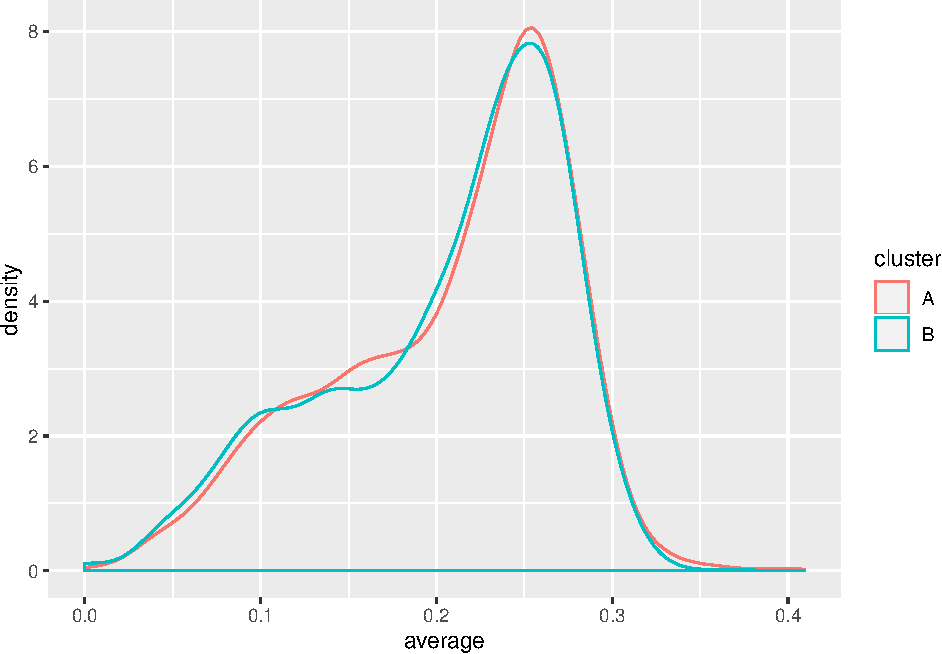
\includegraphics{datadown_files/figure-latex/EM-1.pdf}

\begin{Shaded}
\begin{Highlighting}[]
\KeywordTok{library}\NormalTok{(VGAM)}
\NormalTok{fit_bb_mle <-}\StringTok{ }\ControlFlowTok{function}\NormalTok{(x, n) \{}
  \CommentTok{# dbetabinom.ab 是用n、alpha与beta作为参数的二项贝塔分布的似然度函数}
\NormalTok{  ll <-}\StringTok{ }\ControlFlowTok{function}\NormalTok{(alpha, beta) \{}
    \OperatorTok{-}\KeywordTok{sum}\NormalTok{(}\KeywordTok{dbetabinom.ab}\NormalTok{(x, n, alpha, beta, }\DataTypeTok{log =} \OtherTok{TRUE}\NormalTok{))}
\NormalTok{  \}}
\NormalTok{  m <-}\StringTok{ }\NormalTok{stats4}\OperatorTok{::}\KeywordTok{mle}\NormalTok{(ll, }\DataTypeTok{start =} \KeywordTok{list}\NormalTok{(}\DataTypeTok{alpha =} \DecValTok{3}\NormalTok{, }\DataTypeTok{beta =} \DecValTok{10}\NormalTok{), }\DataTypeTok{method =} \StringTok{"L-BFGS-B"}\NormalTok{,}
                   \DataTypeTok{lower =} \KeywordTok{c}\NormalTok{(}\FloatTok{0.001}\NormalTok{, }\FloatTok{.001}\NormalTok{))}
\NormalTok{  ab <-}\StringTok{ }\NormalTok{stats4}\OperatorTok{::}\KeywordTok{coef}\NormalTok{(m)}
  \KeywordTok{data_frame}\NormalTok{(}\DataTypeTok{alpha =}\NormalTok{ ab[}\DecValTok{1}\NormalTok{], }\DataTypeTok{beta =}\NormalTok{ ab[}\DecValTok{2}\NormalTok{], }\DataTypeTok{number =} \KeywordTok{length}\NormalTok{(x))}
\NormalTok{\}}
\CommentTok{# 看下初始参数}
\KeywordTok{fit_bb_mle}\NormalTok{(starting_data}\OperatorTok{$}\NormalTok{H, starting_data}\OperatorTok{$}\NormalTok{AB)}
\end{Highlighting}
\end{Shaded}

\begin{verbatim}
## # A tibble: 1 x 3
##   alpha  beta number
##   <dbl> <dbl>  <int>
## 1  12.4  44.5   3615
\end{verbatim}

\begin{Shaded}
\begin{Highlighting}[]
\CommentTok{# 看下随机分拆后的参数并生成各分组样本数的先验概率}
\NormalTok{fits <-}\StringTok{ }\NormalTok{starting_data }\OperatorTok
\StringTok{  }\KeywordTok{group_by}\NormalTok{(cluster) }\OperatorTok
\StringTok{  }\KeywordTok{do}\NormalTok{(}\KeywordTok{fit_bb_mle}\NormalTok{(.}\OperatorTok{$}\NormalTok{H, .}\OperatorTok{$}\NormalTok{AB)) }\OperatorTok
\StringTok{  }\KeywordTok{ungroup}\NormalTok{() }\OperatorTok
\StringTok{  }\KeywordTok{mutate}\NormalTok{(}\DataTypeTok{prior =}\NormalTok{ number }\OperatorTok{/}\StringTok{ }\KeywordTok{sum}\NormalTok{(number))}

\NormalTok{fits}
\end{Highlighting}
\end{Shaded}

\begin{verbatim}
## # A tibble: 2 x 5
##   cluster alpha  beta number prior
##   <fct>   <dbl> <dbl>  <int> <dbl>
## 1 A        12.6  45.0   1764 0.488
## 2 B        12.2  44.0   1851 0.512
\end{verbatim}

\begin{itemize}
\tightlist
\item
  算法优化的期望是将这两个分布分拆开,前面一次分拆已经产生微弱差异,下面就通过贝叶斯思想对数据更新这个差异重新分组让两者分开
\end{itemize}

\begin{Shaded}
\begin{Highlighting}[]
\NormalTok{assignments <-}\StringTok{ }\NormalTok{starting_data }\OperatorTok
\StringTok{  }\NormalTok{dplyr}\OperatorTok{::}\KeywordTok{select}\NormalTok{(}\OperatorTok{-}\NormalTok{cluster) }\OperatorTok
\StringTok{  }\KeywordTok{crossing}\NormalTok{(fits) }\OperatorTok
\StringTok{  }\KeywordTok{mutate}\NormalTok{(}\DataTypeTok{likelihood =}\NormalTok{ prior }\OperatorTok{*}\StringTok{ }\NormalTok{VGAM}\OperatorTok{::}\KeywordTok{dbetabinom.ab}\NormalTok{(H, AB, alpha, beta)) }\OperatorTok
\StringTok{  }\KeywordTok{group_by}\NormalTok{(playerID) }\OperatorTok
\StringTok{  }\KeywordTok{top_n}\NormalTok{(}\DecValTok{1}\NormalTok{, likelihood) }\OperatorTok
\StringTok{  }\KeywordTok{ungroup}\NormalTok{()}
\CommentTok{# 去除掉原有分组,根据更新的后验概率重新分组}
\NormalTok{assignments}
\end{Highlighting}
\end{Shaded}

\begin{verbatim}
## # A tibble: 3,615 x 11
##    playerID name      H    AB average cluster alpha  beta number prior
##    <chr>    <chr> <int> <int>   <dbl> <fct>   <dbl> <dbl>  <int> <dbl>
##  1 abbotje~ Jeff~    11    42  0.262  B        12.2  44.0   1851 0.512
##  2 abbotji~ Jim ~     2    21  0.0952 B        12.2  44.0   1851 0.512
##  3 abbotku~ Kurt~   475  1860  0.255  B        12.2  44.0   1851 0.512
##  4 abbotky~ Kyle~     3    31  0.0968 B        12.2  44.0   1851 0.512
##  5 abercre~ Regg~    86   386  0.223  B        12.2  44.0   1851 0.512
##  6 abnersh~ Shaw~   110   531  0.207  B        12.2  44.0   1851 0.512
##  7 abreubo~ Bobb~  1607  5395  0.298  B        12.2  44.0   1851 0.512
##  8 abreuto~ Tony~   129   509  0.253  B        12.2  44.0   1851 0.512
##  9 acevejo~ Jose~     8   101  0.0792 B        12.2  44.0   1851 0.512
## 10 aceveju~ Juan~     6    65  0.0923 B        12.2  44.0   1851 0.512
## # ... with 3,605 more rows, and 1 more variable: likelihood <dbl>
\end{verbatim}

\begin{Shaded}
\begin{Highlighting}[]
\CommentTok{# 观察更新后概率分布}
\KeywordTok{ggplot}\NormalTok{(assignments, }\KeywordTok{aes}\NormalTok{(average, }\DataTypeTok{fill =}\NormalTok{ cluster)) }\OperatorTok{+}
\StringTok{  }\KeywordTok{geom_histogram}\NormalTok{()}
\end{Highlighting}
\end{Shaded}

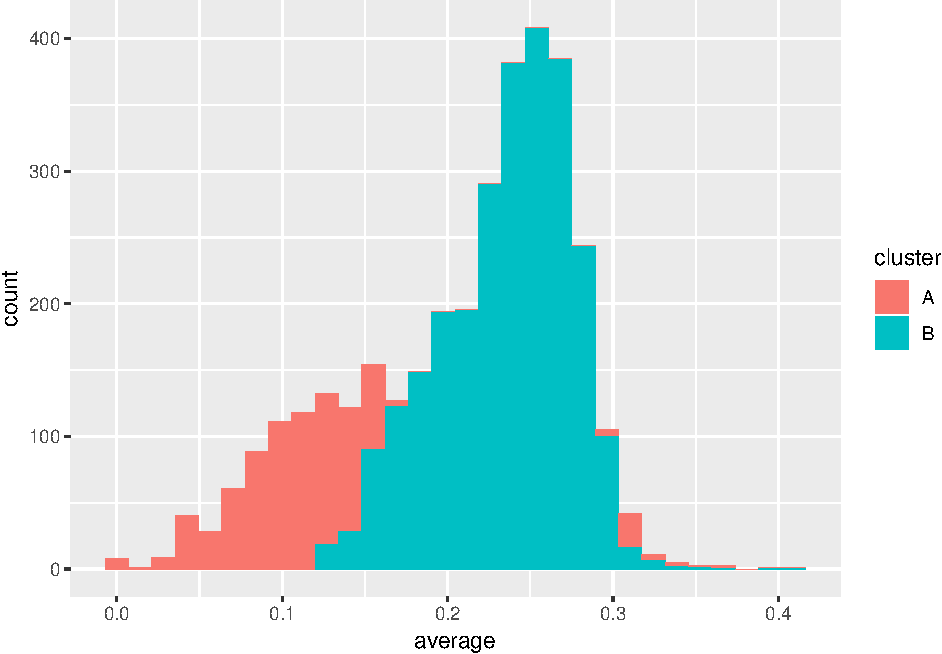
\includegraphics{datadown_files/figure-latex/EMbayes-1.pdf}

\begin{itemize}
\tightlist
\item
  不断重复这个过程,最终分拆数据(其实就是第一步分拆最重要,后面直接收敛了)
\end{itemize}

\begin{Shaded}
\begin{Highlighting}[]
\KeywordTok{set.seed}\NormalTok{(}\DecValTok{1987}\NormalTok{)}

\NormalTok{iterate_em <-}\StringTok{ }\ControlFlowTok{function}\NormalTok{(state, ...) \{}
\NormalTok{  fits <-}\StringTok{ }\NormalTok{state}\OperatorTok{$}\NormalTok{assignments }\OperatorTok
\StringTok{    }\KeywordTok{group_by}\NormalTok{(cluster) }\OperatorTok
\StringTok{    }\KeywordTok{do}\NormalTok{(}\KeywordTok{mutate}\NormalTok{(}\KeywordTok{fit_bb_mle}\NormalTok{(.}\OperatorTok{$}\NormalTok{H, .}\OperatorTok{$}\NormalTok{AB), }\DataTypeTok{number =} \KeywordTok{nrow}\NormalTok{(.))) }\OperatorTok
\StringTok{    }\KeywordTok{ungroup}\NormalTok{() }\OperatorTok
\StringTok{    }\KeywordTok{mutate}\NormalTok{(}\DataTypeTok{prior =}\NormalTok{ number }\OperatorTok{/}\StringTok{ }\KeywordTok{sum}\NormalTok{(number))}

\NormalTok{  assignments <-}\StringTok{ }\NormalTok{assignments }\OperatorTok
\StringTok{    }\NormalTok{dplyr}\OperatorTok{::}\KeywordTok{select}\NormalTok{(playerID}\OperatorTok{:}\NormalTok{average) }\OperatorTok
\StringTok{    }\KeywordTok{crossing}\NormalTok{(fits) }\OperatorTok
\StringTok{    }\KeywordTok{mutate}\NormalTok{(}\DataTypeTok{likelihood =}\NormalTok{ prior }\OperatorTok{*}\StringTok{ }\NormalTok{VGAM}\OperatorTok{::}\KeywordTok{dbetabinom.ab}\NormalTok{(H, AB, alpha, beta)) }\OperatorTok
\StringTok{    }\KeywordTok{group_by}\NormalTok{(playerID) }\OperatorTok
\StringTok{    }\KeywordTok{top_n}\NormalTok{(}\DecValTok{1}\NormalTok{, likelihood) }\OperatorTok
\StringTok{    }\KeywordTok{ungroup}\NormalTok{()}
  
  \KeywordTok{list}\NormalTok{(}\DataTypeTok{assignments =}\NormalTok{ assignments,}
       \DataTypeTok{fits =}\NormalTok{ fits)}
\NormalTok{\}}

\KeywordTok{library}\NormalTok{(purrr)}
\CommentTok{# 使用purrr包存储中间结果}
\NormalTok{iterations <-}\StringTok{ }\KeywordTok{accumulate}\NormalTok{(}\DecValTok{1}\OperatorTok{:}\DecValTok{5}\NormalTok{, iterate_em, }\DataTypeTok{.init =} \KeywordTok{list}\NormalTok{(}\DataTypeTok{assignments =}\NormalTok{ starting_data))}

\NormalTok{assignment_iterations <-}\StringTok{ }\NormalTok{iterations }\OperatorTok
\StringTok{  }\KeywordTok{map_df}\NormalTok{(}\StringTok{"assignments"}\NormalTok{, }\DataTypeTok{.id =} \StringTok{"iteration"}\NormalTok{)}
\CommentTok{# 观察收敛过程}
\NormalTok{assignment_iterations }\OperatorTok
\StringTok{  }\KeywordTok{ggplot}\NormalTok{(}\KeywordTok{aes}\NormalTok{(average, }\DataTypeTok{fill =}\NormalTok{ cluster)) }\OperatorTok{+}
\StringTok{  }\KeywordTok{geom_histogram}\NormalTok{() }\OperatorTok{+}
\StringTok{  }\KeywordTok{facet_wrap}\NormalTok{(}\OperatorTok{~}\StringTok{ }\NormalTok{iteration)}
\end{Highlighting}
\end{Shaded}

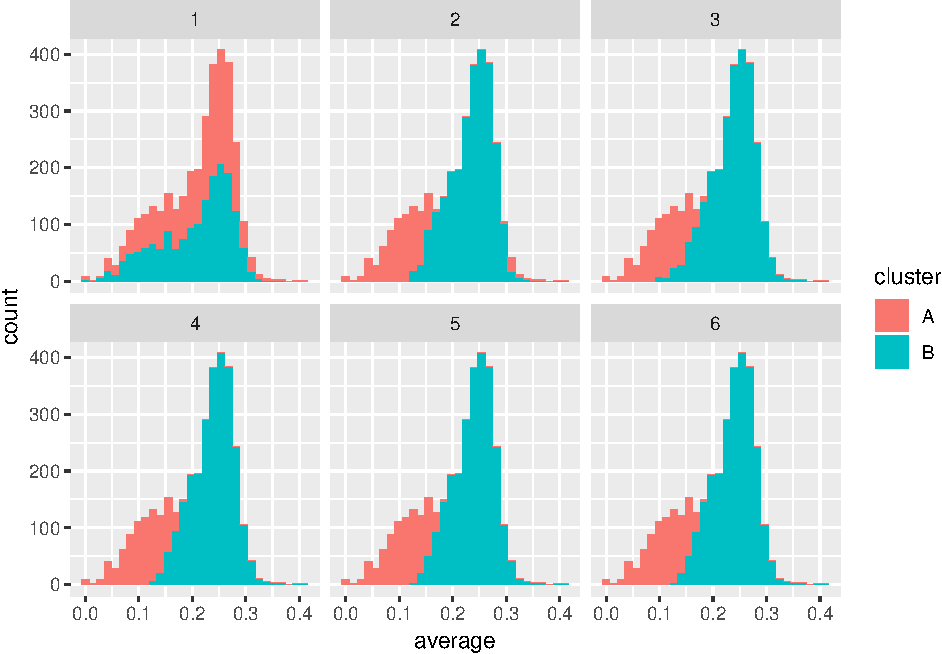
\includegraphics{datadown_files/figure-latex/EMrepeat-1.pdf}

\begin{Shaded}
\begin{Highlighting}[]
\NormalTok{fit_iterations <-}\StringTok{ }\NormalTok{iterations }\OperatorTok
\StringTok{  }\KeywordTok{map_df}\NormalTok{(}\StringTok{"fits"}\NormalTok{, }\DataTypeTok{.id =} \StringTok{"iteration"}\NormalTok{)}
\CommentTok{# 两个分布的收敛过程}
\NormalTok{fit_iterations }\OperatorTok
\StringTok{  }\KeywordTok{crossing}\NormalTok{(}\DataTypeTok{x =} \KeywordTok{seq}\NormalTok{(.}\DecValTok{001}\NormalTok{, }\FloatTok{.4}\NormalTok{, }\FloatTok{.001}\NormalTok{)) }\OperatorTok
\StringTok{  }\KeywordTok{mutate}\NormalTok{(}\DataTypeTok{density =}\NormalTok{ prior }\OperatorTok{*}\StringTok{ }\KeywordTok{dbeta}\NormalTok{(x, alpha, beta)) }\OperatorTok
\StringTok{  }\KeywordTok{ggplot}\NormalTok{(}\KeywordTok{aes}\NormalTok{(x, density, }\DataTypeTok{color =}\NormalTok{ iteration, }\DataTypeTok{group =}\NormalTok{ iteration)) }\OperatorTok{+}
\StringTok{  }\KeywordTok{geom_line}\NormalTok{() }\OperatorTok{+}
\StringTok{  }\KeywordTok{facet_wrap}\NormalTok{(}\OperatorTok{~}\StringTok{ }\NormalTok{cluster)}
\end{Highlighting}
\end{Shaded}

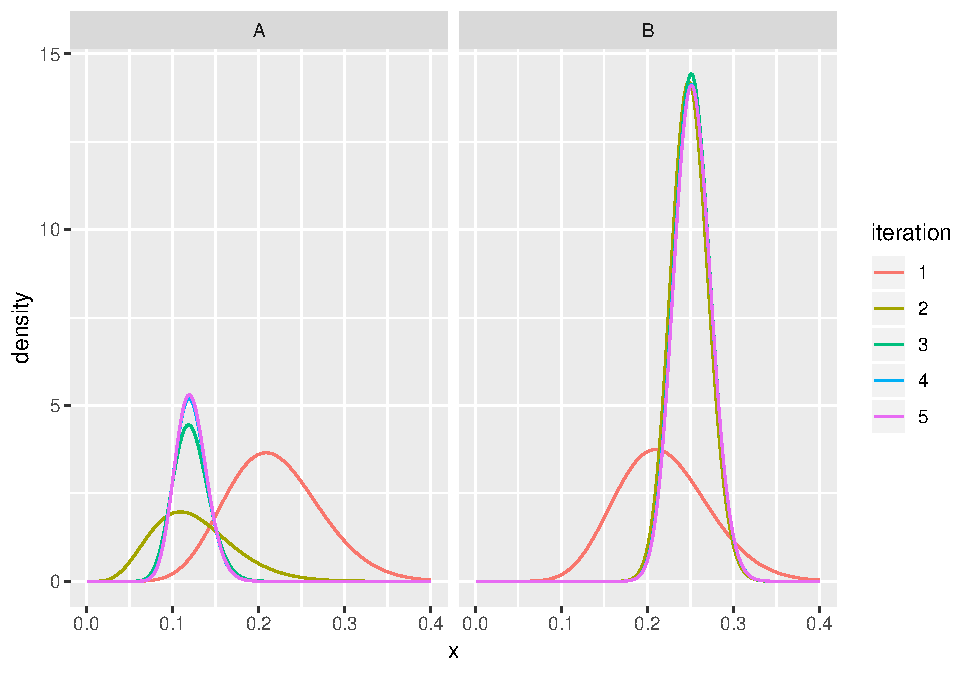
\includegraphics{datadown_files/figure-latex/EMrepeat-2.pdf}

\hypertarget{ux5206ux914d}{%
\subsection{分配}\label{ux5206ux914d}}

\begin{itemize}
\tightlist
\item
  得到每个选手在两个分布中后验概率后要对其进行分配,这里我们认为拆分出的两个分布其实就是是否是击球手的两个分组,由于两组重叠较多,直接分配会有困难
\end{itemize}

\begin{Shaded}
\begin{Highlighting}[]
\CommentTok{# 找6个击球数100的选手进行分配}
\NormalTok{batter100 <-}\StringTok{ }\NormalTok{career }\OperatorTok
\StringTok{  }\KeywordTok{filter}\NormalTok{(AB }\OperatorTok{==}\StringTok{ }\DecValTok{100}\NormalTok{) }\OperatorTok
\StringTok{  }\KeywordTok{arrange}\NormalTok{(average)}
\NormalTok{batter100}
\end{Highlighting}
\end{Shaded}

\begin{verbatim}
## # A tibble: 6 x 8
##   playerID  name            bats      H    AB  year average isPitcher
##   <chr>     <chr>           <fct> <int> <int> <dbl>   <dbl> <lgl>    
## 1 dejesjo01 Jose de Jesus   R        11   100 1990.    0.11 TRUE     
## 2 mahonmi02 Mike Mahoney    R        18   100 2002.    0.18 FALSE    
## 3 cancero01 Robinson Cancel R        20   100 2007.    0.2  FALSE    
## 4 buschmi01 Mike Busch      R        22   100 1996.    0.22 FALSE    
## 5 verdual01 Alex Verdugo    L        24   100 2018.    0.24 FALSE    
## 6 shealry01 Ryan Shealy     R        32   100 2006.    0.32 FALSE
\end{verbatim}

\begin{Shaded}
\begin{Highlighting}[]
\CommentTok{# 前面算法得到的最终结果}
\NormalTok{fit_iterations}
\end{Highlighting}
\end{Shaded}

\begin{verbatim}
## # A tibble: 6 x 6
##   iteration cluster alpha  beta number prior
##   <chr>     <fct>   <dbl> <dbl>  <int> <dbl>
## 1 1         A        12.6  45.0   1764 0.488
## 2 1         B        12.2  44.0   1851 0.512
## 3 2         B        12.4  44.5   3615 1    
## 4 3         B        12.4  44.5   3615 1    
## 5 4         B        12.4  44.5   3615 1    
## 6 5         B        12.4  44.5   3615 1
\end{verbatim}

\begin{Shaded}
\begin{Highlighting}[]
\NormalTok{final_parameters <-}\StringTok{ }\NormalTok{fit_iterations }\OperatorTok
\StringTok{  }\KeywordTok{filter}\NormalTok{(iteration }\OperatorTok{==}\StringTok{ }\DecValTok{1}\NormalTok{)}

\NormalTok{final_parameters}
\end{Highlighting}
\end{Shaded}

\begin{verbatim}
## # A tibble: 2 x 6
##   iteration cluster alpha  beta number prior
##   <chr>     <fct>   <dbl> <dbl>  <int> <dbl>
## 1 1         A        12.6  45.0   1764 0.488
## 2 1         B        12.2  44.0   1851 0.512
\end{verbatim}

\begin{Shaded}
\begin{Highlighting}[]
\CommentTok{# 观察球员位置}
\NormalTok{final_parameters }\OperatorTok
\StringTok{  }\KeywordTok{crossing}\NormalTok{(}\DataTypeTok{x =} \DecValTok{0}\OperatorTok{:}\DecValTok{45}\NormalTok{) }\OperatorTok
\StringTok{  }\KeywordTok{mutate}\NormalTok{(}\DataTypeTok{density =}\NormalTok{ prior }\OperatorTok{*}\StringTok{ }\NormalTok{VGAM}\OperatorTok{::}\KeywordTok{dbetabinom.ab}\NormalTok{(x, }\DecValTok{100}\NormalTok{, alpha, beta)) }\OperatorTok
\StringTok{  }\KeywordTok{ggplot}\NormalTok{(}\KeywordTok{aes}\NormalTok{(x, density)) }\OperatorTok{+}
\StringTok{  }\KeywordTok{geom_line}\NormalTok{(}\KeywordTok{aes}\NormalTok{(}\DataTypeTok{color =}\NormalTok{ cluster)) }\OperatorTok{+}
\StringTok{  }\KeywordTok{geom_vline}\NormalTok{(}\KeywordTok{aes}\NormalTok{(}\DataTypeTok{xintercept =}\NormalTok{ H), }\DataTypeTok{data =}\NormalTok{ batter100, }\DataTypeTok{lty =} \DecValTok{2}\NormalTok{) }\OperatorTok{+}
\StringTok{  }\KeywordTok{geom_text}\NormalTok{(}\KeywordTok{aes}\NormalTok{(}\DataTypeTok{x =}\NormalTok{ H, }\DataTypeTok{y =} \FloatTok{-.022}\NormalTok{, }\DataTypeTok{label =}\NormalTok{ name), }\DataTypeTok{data =}\NormalTok{ batter100, }\DataTypeTok{hjust =} \DecValTok{1}\NormalTok{, }\DataTypeTok{vjust =} \DecValTok{1}\NormalTok{, }\DataTypeTok{angle =} \DecValTok{270}\NormalTok{) }\OperatorTok{+}
\StringTok{  }\KeywordTok{labs}\NormalTok{(}\DataTypeTok{x =} \StringTok{"H (out of 100 at-bats)"}\NormalTok{,}
       \DataTypeTok{y =} \StringTok{"Likelihood of this H out of 100 hits"}\NormalTok{)}
\end{Highlighting}
\end{Shaded}

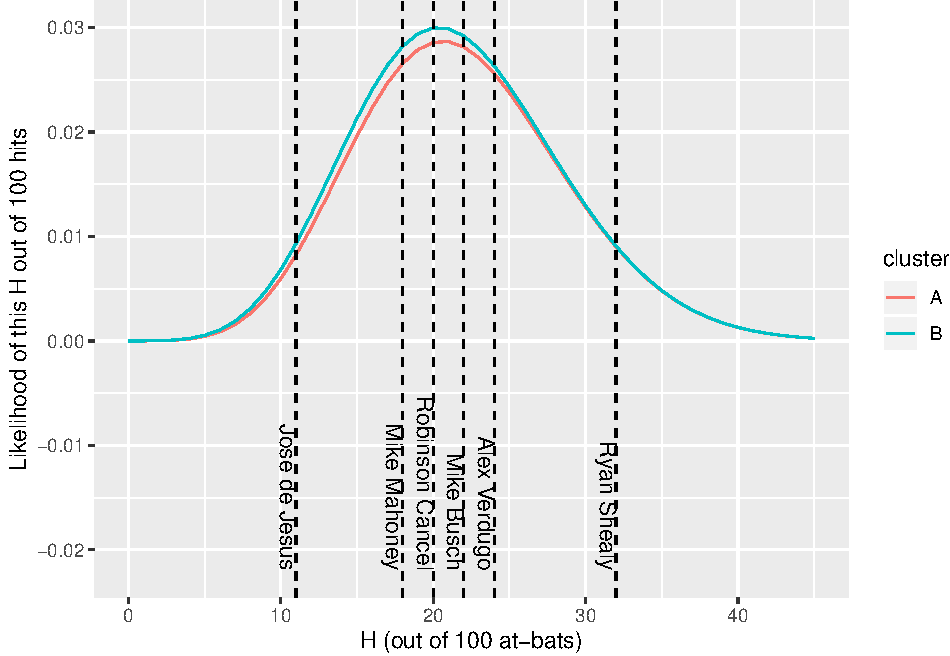
\includegraphics{datadown_files/figure-latex/assign-1.pdf}

\begin{Shaded}
\begin{Highlighting}[]
\CommentTok{# 根据贝叶斯理论,我们可以用在A分组的似然度比上两个分组似然度的和得到后验概率}

\NormalTok{final_parameters }\OperatorTok
\StringTok{  }\KeywordTok{crossing}\NormalTok{(}\DataTypeTok{H =} \DecValTok{1}\OperatorTok{:}\DecValTok{40}\NormalTok{) }\OperatorTok
\StringTok{  }\KeywordTok{transmute}\NormalTok{(H, cluster, }\DataTypeTok{likelihood =}\NormalTok{ prior }\OperatorTok{*}\StringTok{ }\NormalTok{VGAM}\OperatorTok{::}\KeywordTok{dbetabinom.ab}\NormalTok{(H, }\DecValTok{100}\NormalTok{, alpha, beta)) }\OperatorTok
\StringTok{  }\KeywordTok{spread}\NormalTok{(cluster, likelihood) }\OperatorTok
\StringTok{  }\KeywordTok{mutate}\NormalTok{(}\DataTypeTok{probabilityA =}\NormalTok{ A }\OperatorTok{/}\NormalTok{(A }\OperatorTok{+}\StringTok{ }\NormalTok{B)) }\OperatorTok
\StringTok{  }\KeywordTok{ggplot}\NormalTok{(}\KeywordTok{aes}\NormalTok{(H, probabilityA)) }\OperatorTok{+}
\StringTok{  }\KeywordTok{geom_line}\NormalTok{() }\OperatorTok{+}
\StringTok{  }\KeywordTok{geom_vline}\NormalTok{(}\KeywordTok{aes}\NormalTok{(}\DataTypeTok{xintercept =}\NormalTok{ H), }\DataTypeTok{data =}\NormalTok{ batter100, }\DataTypeTok{lty =} \DecValTok{2}\NormalTok{) }\OperatorTok{+}
\StringTok{  }\KeywordTok{geom_text}\NormalTok{(}\KeywordTok{aes}\NormalTok{(}\DataTypeTok{x =}\NormalTok{ H, }\DataTypeTok{y =} \DecValTok{0}\NormalTok{, }\DataTypeTok{label =}\NormalTok{ name), }\DataTypeTok{data =}\NormalTok{ batter100, }\DataTypeTok{hjust =} \DecValTok{1}\NormalTok{, }\DataTypeTok{vjust =} \DecValTok{1}\NormalTok{, }\DataTypeTok{angle =} \DecValTok{270}\NormalTok{) }\OperatorTok{+}
\StringTok{  }\KeywordTok{labs}\NormalTok{(}\DataTypeTok{x =} \StringTok{"H (out of 100 at-bats)"}\NormalTok{,}
        \DataTypeTok{y =} \StringTok{"(Likelihood if pitcher) / (Likelihood if pitcher + Likelihood if not)"}\NormalTok{,}
        \DataTypeTok{title =} \StringTok{"Posterior probability a player is in the pitcher cluster"}\NormalTok{)}
\end{Highlighting}
\end{Shaded}

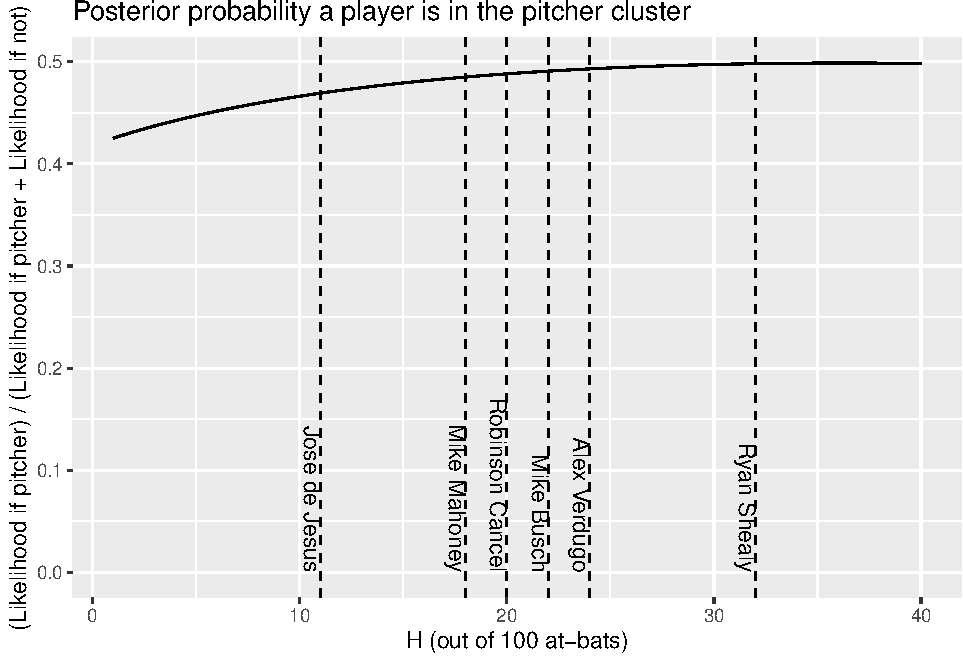
\includegraphics{datadown_files/figure-latex/assign-2.pdf}

\begin{itemize}
\tightlist
\item
  通过构建后验概率,我们可以直接对结果基于概率进行分组
\end{itemize}

\begin{Shaded}
\begin{Highlighting}[]
\NormalTok{career_likelihoods <-}\StringTok{ }\NormalTok{career }\OperatorTok
\StringTok{  }\KeywordTok{filter}\NormalTok{(AB }\OperatorTok{>}\StringTok{ }\DecValTok{20}\NormalTok{) }\OperatorTok
\StringTok{  }\KeywordTok{crossing}\NormalTok{(final_parameters) }\OperatorTok
\StringTok{  }\KeywordTok{mutate}\NormalTok{(}\DataTypeTok{likelihood =}\NormalTok{ prior }\OperatorTok{*}\StringTok{ }\NormalTok{VGAM}\OperatorTok{::}\KeywordTok{dbetabinom.ab}\NormalTok{(H, AB, alpha, beta)) }\OperatorTok
\StringTok{  }\KeywordTok{group_by}\NormalTok{(playerID) }\OperatorTok
\StringTok{  }\KeywordTok{mutate}\NormalTok{(}\DataTypeTok{posterior =}\NormalTok{ likelihood }\OperatorTok{/}\StringTok{ }\KeywordTok{sum}\NormalTok{(likelihood))}

\NormalTok{career_assignments <-}\StringTok{ }\NormalTok{career_likelihoods }\OperatorTok
\StringTok{  }\KeywordTok{top_n}\NormalTok{(}\DecValTok{1}\NormalTok{, posterior) }\OperatorTok
\StringTok{  }\KeywordTok{ungroup}\NormalTok{()}
\CommentTok{# 对比这种分组与实际数据的结果}
\NormalTok{career_assignments }\OperatorTok
\StringTok{  }\KeywordTok{filter}\NormalTok{(posterior }\OperatorTok{>}\StringTok{ }\FloatTok{.8}\NormalTok{) }\OperatorTok
\StringTok{  }\KeywordTok{count}\NormalTok{(isPitcher, cluster) }\OperatorTok
\StringTok{  }\KeywordTok{spread}\NormalTok{(cluster, n)}
\end{Highlighting}
\end{Shaded}

\begin{verbatim}
## # A tibble: 2 x 2
##   isPitcher     B
##   <lgl>     <int>
## 1 FALSE      2510
## 2 TRUE       1073
\end{verbatim}

\begin{itemize}
\tightlist
\item
  这样基于对概率分布的观察,我们可以实现有现实意义的分组,对分组的改进则需要对数据的进一步理解
\end{itemize}

\hypertarget{ux7ecfux9a8cux8d1dux53f6ux65afux6536ux7f29}{%
\subsection{经验贝叶斯收缩}\label{ux7ecfux9a8cux8d1dux53f6ux65afux6536ux7f29}}

\begin{itemize}
\tightlist
\item
  混合模型下前面所做的工作都需要重新考虑
\end{itemize}

\begin{Shaded}
\begin{Highlighting}[]
\CommentTok{# 观察击球数100选手的后验概率分布}
\NormalTok{batting_data <-}\StringTok{ }\NormalTok{career_likelihoods }\OperatorTok
\StringTok{  }\KeywordTok{ungroup}\NormalTok{() }\OperatorTok
\StringTok{  }\KeywordTok{filter}\NormalTok{(AB }\OperatorTok{==}\StringTok{ }\DecValTok{100}\NormalTok{) }\OperatorTok
\StringTok{  }\KeywordTok{mutate}\NormalTok{(}\DataTypeTok{name =} \KeywordTok{paste0}\NormalTok{(name, }\StringTok{" ("}\NormalTok{, H, }\StringTok{"/"}\NormalTok{, AB, }\StringTok{")"}\NormalTok{),}
         \DataTypeTok{name =} \KeywordTok{reorder}\NormalTok{(name, H),}
         \DataTypeTok{alpha1 =}\NormalTok{ H }\OperatorTok{+}\StringTok{ }\NormalTok{alpha,}
         \DataTypeTok{beta1 =}\NormalTok{ AB }\OperatorTok{-}\StringTok{ }\NormalTok{H }\OperatorTok{+}\StringTok{ }\NormalTok{beta)}

\NormalTok{batting_data }\OperatorTok
\StringTok{  }\KeywordTok{crossing}\NormalTok{(}\DataTypeTok{x =} \KeywordTok{seq}\NormalTok{(}\DecValTok{0}\NormalTok{, }\FloatTok{.4}\NormalTok{, }\FloatTok{.001}\NormalTok{)) }\OperatorTok
\StringTok{  }\KeywordTok{mutate}\NormalTok{(}\DataTypeTok{posterior_density =}\NormalTok{ posterior }\OperatorTok{*}\StringTok{ }\KeywordTok{dbeta}\NormalTok{(x, alpha1, beta1)) }\OperatorTok
\StringTok{  }\KeywordTok{group_by}\NormalTok{(name, x) }\OperatorTok
\StringTok{  }\KeywordTok{summarize}\NormalTok{(}\DataTypeTok{posterior_density =} \KeywordTok{sum}\NormalTok{(posterior_density)) }\OperatorTok
\StringTok{  }\KeywordTok{ggplot}\NormalTok{(}\KeywordTok{aes}\NormalTok{(x, posterior_density, }\DataTypeTok{color =}\NormalTok{ name)) }\OperatorTok{+}
\StringTok{  }\KeywordTok{geom_line}\NormalTok{(}\DataTypeTok{show.legend =} \OtherTok{FALSE}\NormalTok{) }\OperatorTok{+}
\StringTok{  }\KeywordTok{geom_vline}\NormalTok{(}\KeywordTok{aes}\NormalTok{(}\DataTypeTok{xintercept =}\NormalTok{ average), }\DataTypeTok{data =}\NormalTok{ batting_data, }\DataTypeTok{lty =} \DecValTok{2}\NormalTok{) }\OperatorTok{+}
\StringTok{  }\KeywordTok{facet_wrap}\NormalTok{(}\OperatorTok{~}\StringTok{ }\NormalTok{name) }\OperatorTok{+}
\StringTok{  }\KeywordTok{labs}\NormalTok{(}\DataTypeTok{x =} \StringTok{"Batting average (actual average shown as dashed line)"}\NormalTok{,}
       \DataTypeTok{y =} \StringTok{"Posterior density after updating"}\NormalTok{)}
\end{Highlighting}
\end{Shaded}

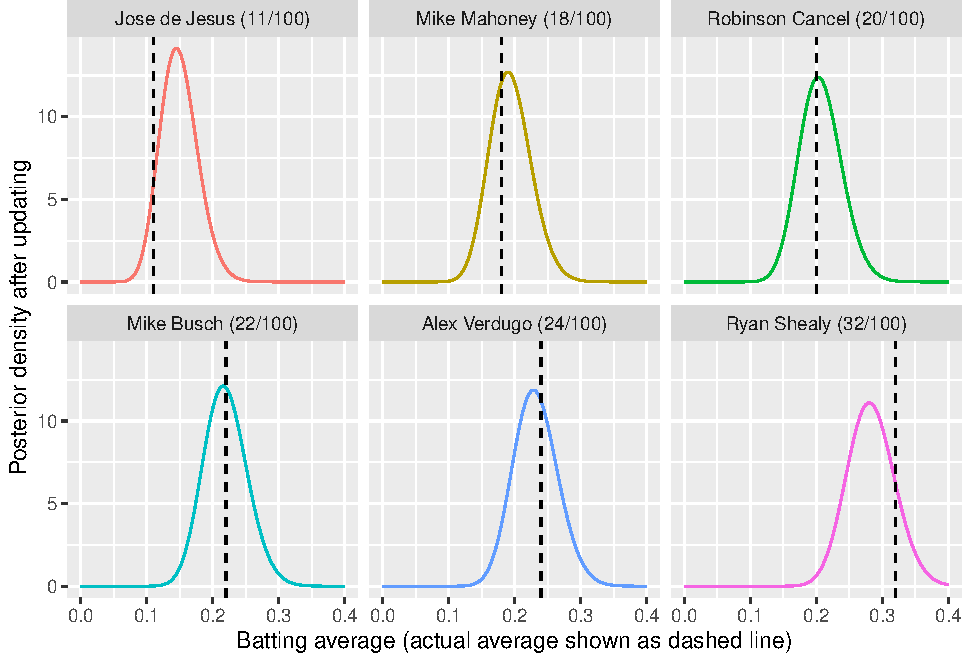
\includegraphics{datadown_files/figure-latex/ebayesem-1.pdf}

\begin{itemize}
\tightlist
\item
  此时不太好判断属于哪一分布,可采用后验概率对平均分布进行加权
\end{itemize}

\begin{Shaded}
\begin{Highlighting}[]
\NormalTok{eb_shrinkage <-}\StringTok{ }\NormalTok{career_likelihoods }\OperatorTok
\StringTok{  }\KeywordTok{mutate}\NormalTok{(}\DataTypeTok{shrunken_average =}\NormalTok{ (H }\OperatorTok{+}\StringTok{ }\NormalTok{alpha) }\OperatorTok{/}\StringTok{ }\NormalTok{(AB }\OperatorTok{+}\StringTok{ }\NormalTok{alpha }\OperatorTok{+}\StringTok{ }\NormalTok{beta)) }\OperatorTok
\StringTok{  }\KeywordTok{group_by}\NormalTok{(playerID) }\OperatorTok
\StringTok{  }\KeywordTok{summarize}\NormalTok{(}\DataTypeTok{shrunken_average =} \KeywordTok{sum}\NormalTok{(posterior }\OperatorTok{*}\StringTok{ }\NormalTok{shrunken_average))}
\CommentTok{# 观察加权分布}
\NormalTok{eb_shrinkage }\OperatorTok
\StringTok{  }\KeywordTok{inner_join}\NormalTok{(career) }\OperatorTok
\StringTok{  }\KeywordTok{filter}\NormalTok{(AB }\OperatorTok{>}\StringTok{ }\DecValTok{50}\NormalTok{) }\OperatorTok
\StringTok{  }\KeywordTok{gather}\NormalTok{(type, value, average, shrunken_average) }\OperatorTok
\StringTok{  }\KeywordTok{mutate}\NormalTok{(}\DataTypeTok{type =} \KeywordTok{ifelse}\NormalTok{(type }\OperatorTok{==}\StringTok{ "average"}\NormalTok{, }\StringTok{"Raw batting average"}\NormalTok{, }\StringTok{"Average posterior"}\NormalTok{),}
         \DataTypeTok{type =} \KeywordTok{relevel}\NormalTok{(}\KeywordTok{factor}\NormalTok{(type), }\StringTok{"Raw batting average"}\NormalTok{)) }\OperatorTok
\StringTok{  }\KeywordTok{ggplot}\NormalTok{(}\KeywordTok{aes}\NormalTok{(AB, value)) }\OperatorTok{+}
\StringTok{  }\KeywordTok{geom_point}\NormalTok{() }\OperatorTok{+}
\StringTok{  }\KeywordTok{facet_wrap}\NormalTok{(}\OperatorTok{~}\StringTok{ }\NormalTok{type) }\OperatorTok{+}
\StringTok{  }\KeywordTok{scale_x_log10}\NormalTok{() }\OperatorTok{+}
\StringTok{  }\KeywordTok{ylab}\NormalTok{(}\StringTok{"Estimate"}\NormalTok{)}
\end{Highlighting}
\end{Shaded}

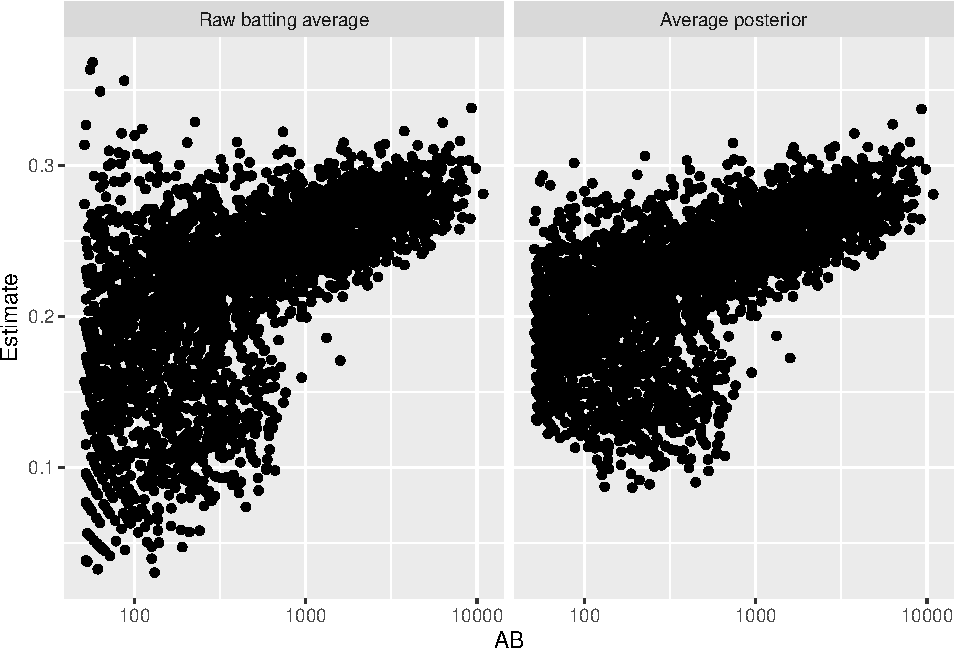
\includegraphics{datadown_files/figure-latex/weightdist-1.pdf}
- 收敛后的分布会朝向两个中心而不是一个,并非所有之前的方法(例如区间估计)都可以适用到混合模型里,需要根据实际情况进行分析

\hypertarget{ux6a21ux62dfux9a8cux8bc1ux7ed3ux679c}{%
\section{模拟验证结果}\label{ux6a21ux62dfux9a8cux8bc1ux7ed3ux679c}}

\begin{itemize}
\tightlist
\item
  上面的经验贝叶斯推断大都是给出的结果,我们需要对其进行模拟验证
\end{itemize}

\begin{Shaded}
\begin{Highlighting}[]
\NormalTok{pitchers <-}\StringTok{ }\NormalTok{Pitching }\OperatorTok
\StringTok{  }\KeywordTok{group_by}\NormalTok{(playerID) }\OperatorTok
\StringTok{  }\KeywordTok{summarize}\NormalTok{(}\DataTypeTok{gamesPitched =} \KeywordTok{sum}\NormalTok{(G)) }\OperatorTok
\StringTok{  }\KeywordTok{filter}\NormalTok{(gamesPitched }\OperatorTok{>}\StringTok{ }\DecValTok{3}\NormalTok{)}
\NormalTok{career <-}\StringTok{ }\NormalTok{Batting }\OperatorTok
\StringTok{  }\KeywordTok{filter}\NormalTok{(AB }\OperatorTok{>}\StringTok{ }\DecValTok{0}\NormalTok{) }\OperatorTok
\StringTok{  }\KeywordTok{anti_join}\NormalTok{(pitchers, }\DataTypeTok{by =} \StringTok{"playerID"}\NormalTok{) }\OperatorTok
\StringTok{  }\KeywordTok{group_by}\NormalTok{(playerID) }\OperatorTok
\StringTok{  }\KeywordTok{summarize}\NormalTok{(}\DataTypeTok{H =} \KeywordTok{sum}\NormalTok{(H), }\DataTypeTok{AB =} \KeywordTok{sum}\NormalTok{(AB))}
\CommentTok{# 从数据中找到贝塔分布的两个参数}
\KeywordTok{library}\NormalTok{(ebbr)}
\NormalTok{prior <-}\StringTok{ }\NormalTok{career }\OperatorTok
\StringTok{  }\KeywordTok{ebb_fit_prior}\NormalTok{(H, AB)}

\NormalTok{prior}
\end{Highlighting}
\end{Shaded}

\begin{verbatim}
## Empirical Bayes binomial fit with method mle 
## Parameters:
## # A tibble: 1 x 2
##   alpha  beta
##   <dbl> <dbl>
## 1  72.9  218.
\end{verbatim}

\begin{Shaded}
\begin{Highlighting}[]
\CommentTok{# 用这两个参数生成球员的击球概率}
\NormalTok{alpha0 <-}\StringTok{ }\KeywordTok{tidy}\NormalTok{(prior)}\OperatorTok{$}\NormalTok{alpha}
\NormalTok{beta0 <-}\StringTok{ }\KeywordTok{tidy}\NormalTok{(prior)}\OperatorTok{$}\NormalTok{beta}

\KeywordTok{qplot}\NormalTok{(}\KeywordTok{rbeta}\NormalTok{(}\DecValTok{10000}\NormalTok{, alpha0, beta0))}
\end{Highlighting}
\end{Shaded}

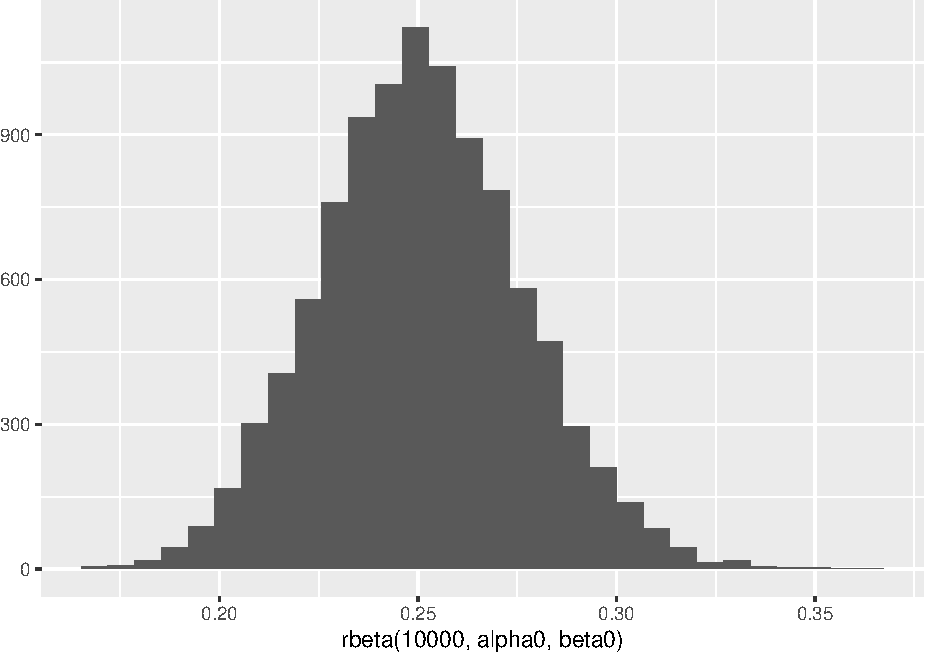
\includegraphics{datadown_files/figure-latex/dtpre-1.pdf}

\begin{Shaded}
\begin{Highlighting}[]
\CommentTok{# 击球数使用原始数据}
\KeywordTok{ggplot}\NormalTok{(career, }\KeywordTok{aes}\NormalTok{(AB)) }\OperatorTok{+}
\StringTok{  }\KeywordTok{geom_histogram}\NormalTok{() }\OperatorTok{+}
\StringTok{  }\KeywordTok{scale_x_log10}\NormalTok{()}
\end{Highlighting}
\end{Shaded}

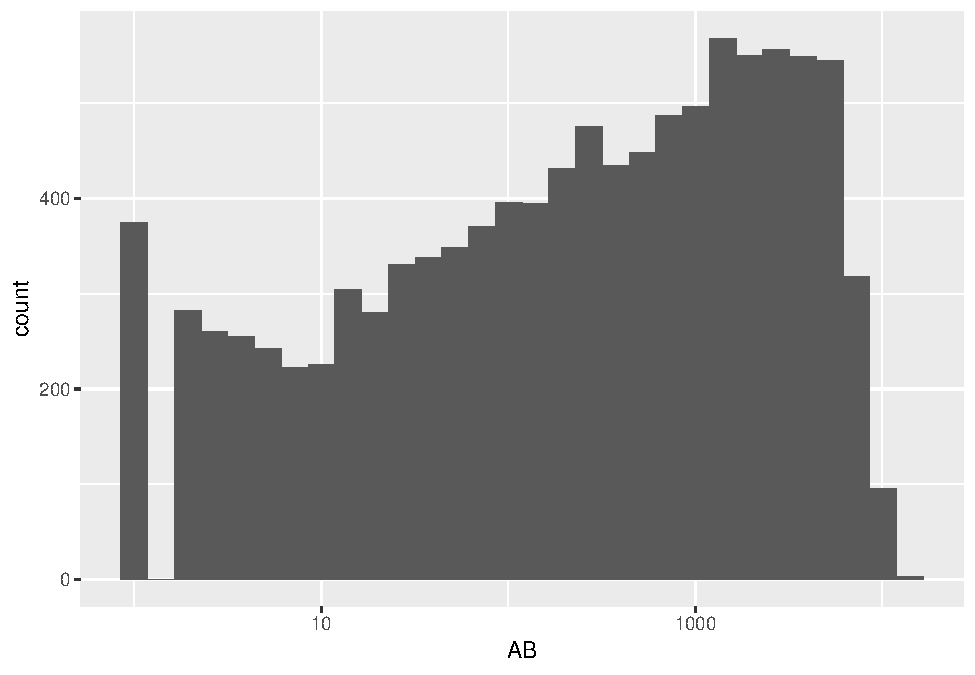
\includegraphics{datadown_files/figure-latex/dtpre-2.pdf}

\begin{Shaded}
\begin{Highlighting}[]
\CommentTok{# 构建仿真数据}
\KeywordTok{set.seed}\NormalTok{(}\DecValTok{2017}\NormalTok{)}

\NormalTok{career_sim <-}\StringTok{ }\NormalTok{career }\OperatorTok
\StringTok{  }\KeywordTok{mutate}\NormalTok{(}\DataTypeTok{p =} \KeywordTok{rbeta}\NormalTok{(}\KeywordTok{n}\NormalTok{(), alpha0, beta0),}
         \DataTypeTok{H =} \KeywordTok{rbinom}\NormalTok{(}\KeywordTok{n}\NormalTok{(), AB, p))}

\NormalTok{career_sim}
\end{Highlighting}
\end{Shaded}

\begin{verbatim}
## # A tibble: 10,800 x 4
##    playerID      H    AB     p
##    <chr>     <int> <int> <dbl>
##  1 aaronha01  3665 12364 0.298
##  2 aaronto01   249   944 0.249
##  3 abadan01      6    21 0.273
##  4 abadijo01    10    49 0.198
##  5 abbated01   790  3044 0.249
##  6 abbeych01   460  1756 0.264
##  7 abbotda01     3     7 0.191
##  8 abbotfr01   132   513 0.251
##  9 abbotje01   151   596 0.243
## 10 abbotku01   535  2044 0.261
## # ... with 10,790 more rows
\end{verbatim}

\hypertarget{ux6a21ux62dfux5bf9ux5206ux5e03ux53c2ux6570ux7684ux4f30ux8ba1}{%
\subsection{模拟对分布参数的估计}\label{ux6a21ux62dfux5bf9ux5206ux5e03ux53c2ux6570ux7684ux4f30ux8ba1}}

\begin{itemize}
\tightlist
\item
  生产数据后我们可以估计分布参数,看能否与模拟值对应
\end{itemize}

\begin{Shaded}
\begin{Highlighting}[]
\NormalTok{career_sim_eb <-}\StringTok{ }\NormalTok{career_sim }\OperatorTok
\StringTok{  }\KeywordTok{add_ebb_estimate}\NormalTok{(H, AB)}

\NormalTok{career_sim_gathered <-}\StringTok{ }\NormalTok{career_sim_eb }\OperatorTok
\StringTok{  }\KeywordTok{rename}\NormalTok{(}\DataTypeTok{Shrunken =}\NormalTok{ .fitted, }\DataTypeTok{Raw =}\NormalTok{ .raw) }\OperatorTok
\StringTok{  }\KeywordTok{gather}\NormalTok{(type, estimate, Shrunken, Raw)}
\CommentTok{# 观察是否能收敛数据}
\NormalTok{career_sim_gathered }\OperatorTok
\StringTok{  }\KeywordTok{filter}\NormalTok{(AB }\OperatorTok{>=}\StringTok{ }\DecValTok{10}\NormalTok{) }\OperatorTok
\StringTok{  }\KeywordTok{ggplot}\NormalTok{(}\KeywordTok{aes}\NormalTok{(p, estimate, }\DataTypeTok{color =}\NormalTok{ AB)) }\OperatorTok{+}
\StringTok{  }\KeywordTok{geom_point}\NormalTok{() }\OperatorTok{+}
\StringTok{  }\KeywordTok{geom_abline}\NormalTok{(}\DataTypeTok{color =} \StringTok{"red"}\NormalTok{) }\OperatorTok{+}
\StringTok{  }\KeywordTok{geom_smooth}\NormalTok{(}\DataTypeTok{method =} \StringTok{"lm"}\NormalTok{, }\DataTypeTok{color =} \StringTok{"white"}\NormalTok{, }\DataTypeTok{lty =} \DecValTok{2}\NormalTok{, }\DataTypeTok{se =} \OtherTok{FALSE}\NormalTok{) }\OperatorTok{+}
\StringTok{  }\KeywordTok{scale_color_continuous}\NormalTok{(}\DataTypeTok{trans =} \StringTok{"log"}\NormalTok{, }\DataTypeTok{breaks =} \KeywordTok{c}\NormalTok{(}\DecValTok{10}\NormalTok{, }\DecValTok{100}\NormalTok{, }\DecValTok{1000}\NormalTok{, }\DecValTok{10000}\NormalTok{)) }\OperatorTok{+}
\StringTok{  }\KeywordTok{facet_wrap}\NormalTok{(}\OperatorTok{~}\StringTok{ }\NormalTok{type) }\OperatorTok{+}
\StringTok{  }\KeywordTok{labs}\NormalTok{(}\DataTypeTok{x =} \StringTok{"True batting average (p)"}\NormalTok{,}
       \DataTypeTok{y =} \StringTok{"Raw or shrunken batting average"}\NormalTok{,}
       \DataTypeTok{title =} \StringTok{"Empirical Bayes shrinkage reduces variance, but causes bias"}\NormalTok{,}
       \DataTypeTok{subtitle =} \StringTok{"Red line is x = y; dashed white line is a linear fit"}\NormalTok{)}
\end{Highlighting}
\end{Shaded}

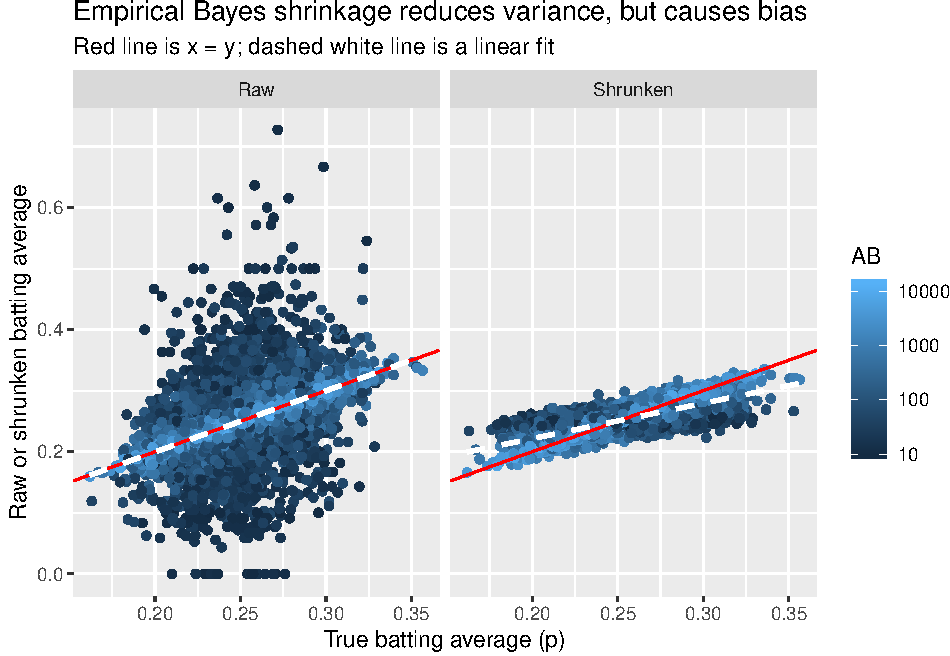
\includegraphics{datadown_files/figure-latex/simhpara-1.pdf}

\begin{itemize}
\item
  我们可以看到,估计方差有了一定收敛,但出现了一定偏差,可参考统计学习中方差-偏差权衡的描述
\item
  可以用均方误来衡量,此处虽牺牲了偏差,但整体误差降低了
\end{itemize}

\[\mbox{MSE}=\frac{1}{n}\sum_{1}^{n}(p-\hat{p})^2\]

\begin{Shaded}
\begin{Highlighting}[]
\NormalTok{career_sim_gathered }\OperatorTok
\StringTok{  }\KeywordTok{group_by}\NormalTok{(type) }\OperatorTok
\StringTok{  }\KeywordTok{summarize}\NormalTok{(}\DataTypeTok{mse =} \KeywordTok{mean}\NormalTok{((estimate }\OperatorTok{-}\StringTok{ }\NormalTok{p) }\OperatorTok{^}\StringTok{ }\DecValTok{2}\NormalTok{))}
\end{Highlighting}
\end{Shaded}

\begin{verbatim}
## # A tibble: 2 x 2
##   type          mse
##   <chr>       <dbl>
## 1 Raw      0.0152  
## 2 Shrunken 0.000347
\end{verbatim}

\begin{itemize}
\tightlist
\item
  注意到击球数可能影响收敛,所以可以探索其对均方误的影响
\end{itemize}

\begin{Shaded}
\begin{Highlighting}[]
\NormalTok{metric_by_bin <-}\StringTok{ }\NormalTok{career_sim_gathered }\OperatorTok
\StringTok{  }\KeywordTok{group_by}\NormalTok{(type, }\DataTypeTok{AB =} \DecValTok{10} \OperatorTok{^}\StringTok{ }\NormalTok{(}\KeywordTok{round}\NormalTok{(}\KeywordTok{log10}\NormalTok{(AB)))) }\OperatorTok
\StringTok{  }\KeywordTok{summarize}\NormalTok{(}\DataTypeTok{mse =} \KeywordTok{mean}\NormalTok{((estimate }\OperatorTok{-}\StringTok{ }\NormalTok{p) }\OperatorTok{^}\StringTok{ }\DecValTok{2}\NormalTok{))}

\KeywordTok{ggplot}\NormalTok{(metric_by_bin, }\KeywordTok{aes}\NormalTok{(AB, mse, }\DataTypeTok{color =}\NormalTok{ type)) }\OperatorTok{+}
\StringTok{  }\KeywordTok{geom_line}\NormalTok{() }\OperatorTok{+}
\StringTok{  }\KeywordTok{scale_x_log10}\NormalTok{() }\OperatorTok{+}
\StringTok{  }\KeywordTok{scale_y_log10}\NormalTok{() }\OperatorTok{+}
\StringTok{  }\KeywordTok{labs}\NormalTok{(}\DataTypeTok{x =} \StringTok{"Number of at-bats (AB)"}\NormalTok{,}
       \DataTypeTok{y =} \StringTok{"Mean-squared-error within this bin (note log scale)"}\NormalTok{,}
       \DataTypeTok{title =} \StringTok{"Mean squared error is higher with raw estimate, especially for low AB"}\NormalTok{)}
\end{Highlighting}
\end{Shaded}

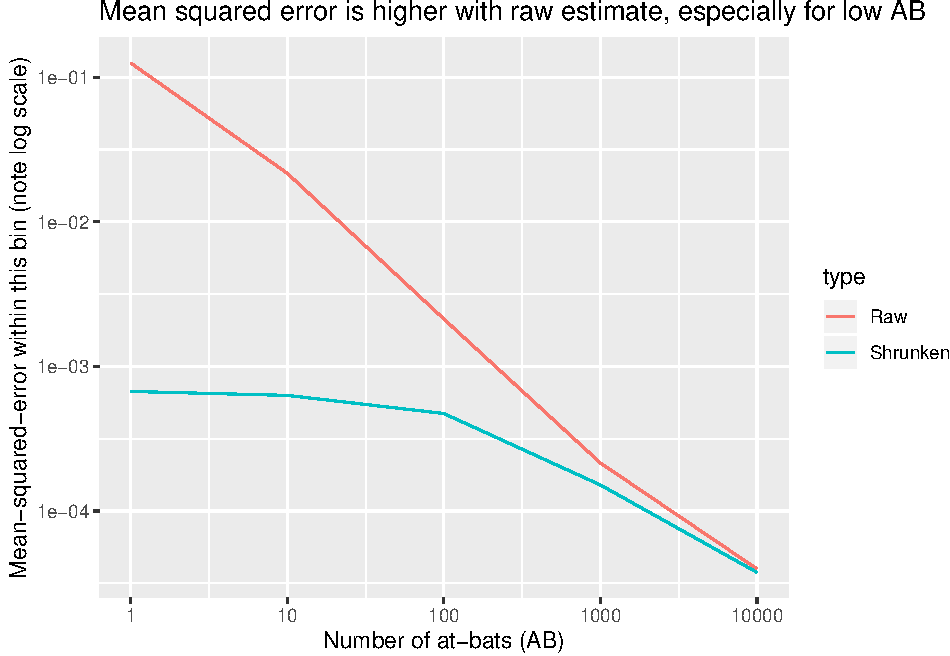
\includegraphics{datadown_files/figure-latex/simAB-1.pdf}

\begin{itemize}
\tightlist
\item
  击球数越多,均方误越低,此时可进一步探索
\end{itemize}

\begin{Shaded}
\begin{Highlighting}[]
\KeywordTok{library}\NormalTok{(scales)}
\CommentTok{# 观察斜率p值变化}
\NormalTok{career_sim_gathered }\OperatorTok
\StringTok{  }\KeywordTok{mutate}\NormalTok{(}\DataTypeTok{AB =} \DecValTok{10} \OperatorTok{^}\StringTok{ }\NormalTok{(}\KeywordTok{round}\NormalTok{(}\KeywordTok{log10}\NormalTok{(AB)))) }\OperatorTok
\StringTok{  }\KeywordTok{filter}\NormalTok{(AB }\OperatorTok{>}\StringTok{ }\DecValTok{1}\NormalTok{) }\OperatorTok
\StringTok{  }\KeywordTok{nest}\NormalTok{(}\OperatorTok{-}\NormalTok{type, }\OperatorTok{-}\NormalTok{AB) }\OperatorTok
\StringTok{  }\KeywordTok{mutate}\NormalTok{(}\DataTypeTok{model=}\KeywordTok{map}\NormalTok{(data, }\OperatorTok{~}\StringTok{ }\KeywordTok{tidy}\NormalTok{(}\KeywordTok{lm}\NormalTok{(estimate }\OperatorTok{~}\StringTok{ }\NormalTok{p, .)))) }\OperatorTok
\StringTok{  }\KeywordTok{unnest}\NormalTok{(model) }\OperatorTok
\StringTok{  }\KeywordTok{filter}\NormalTok{(term }\OperatorTok{==}\StringTok{ "p"}\NormalTok{) }\OperatorTok
\StringTok{  }\KeywordTok{ggplot}\NormalTok{(}\KeywordTok{aes}\NormalTok{(AB, estimate, }\DataTypeTok{color =}\NormalTok{ type)) }\OperatorTok{+}
\StringTok{  }\KeywordTok{geom_line}\NormalTok{() }\OperatorTok{+}
\StringTok{  }\KeywordTok{scale_x_log10}\NormalTok{(}\DataTypeTok{breaks =} \KeywordTok{c}\NormalTok{(}\DecValTok{10}\NormalTok{, }\DecValTok{100}\NormalTok{, }\DecValTok{1000}\NormalTok{, }\DecValTok{10000}\NormalTok{)) }\OperatorTok{+}
\StringTok{  }\KeywordTok{geom_hline}\NormalTok{(}\DataTypeTok{yintercept =} \DecValTok{1}\NormalTok{, }\DataTypeTok{lty =} \DecValTok{2}\NormalTok{) }\OperatorTok{+}
\StringTok{  }\KeywordTok{labs}\NormalTok{(}\DataTypeTok{x =} \StringTok{"Number of at-bats (AB)"}\NormalTok{,}
       \DataTypeTok{y =} \StringTok{"Slope of estimate/p within this bin"}\NormalTok{,}
       \DataTypeTok{title =} \StringTok{"Shrunken estimates introduce bias for low AB"}\NormalTok{,}
       \DataTypeTok{subtitle =} \StringTok{"Note that an unbiased estimate would have a slope of 0"}\NormalTok{)}
\end{Highlighting}
\end{Shaded}

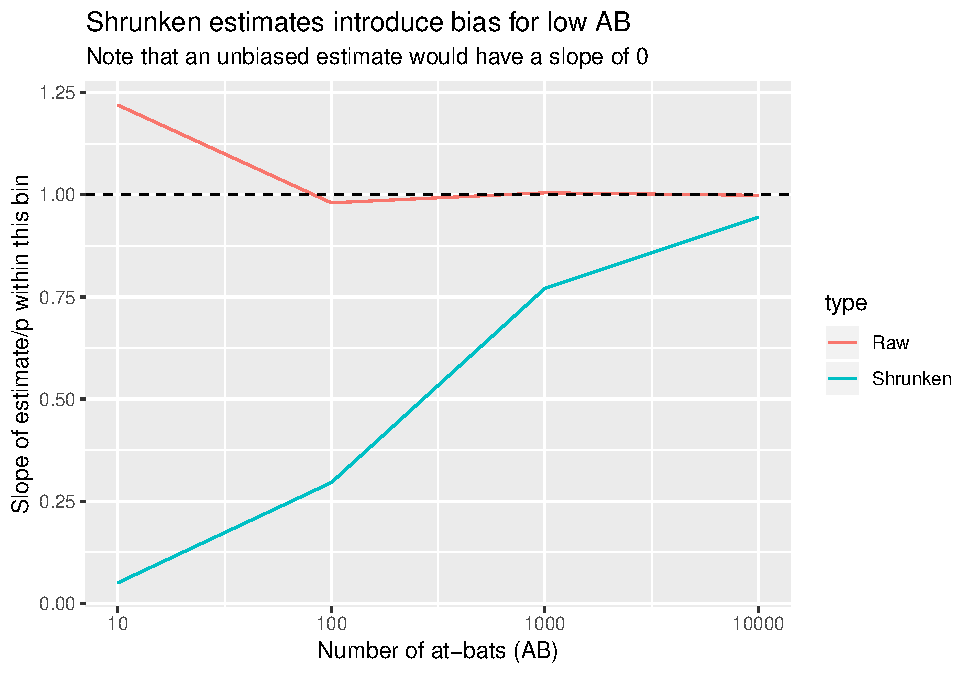
\includegraphics{datadown_files/figure-latex/simp-1.pdf}

\begin{Shaded}
\begin{Highlighting}[]
\CommentTok{# 分层}
\NormalTok{career_sim_gathered }\OperatorTok
\StringTok{  }\KeywordTok{mutate}\NormalTok{(}\DataTypeTok{ab_bin =} \KeywordTok{cut}\NormalTok{(AB, }\KeywordTok{c}\NormalTok{(}\DecValTok{0}\NormalTok{, }\DecValTok{10}\NormalTok{, }\DecValTok{100}\NormalTok{, }\DecValTok{1000}\NormalTok{, }\OtherTok{Inf}\NormalTok{),}
                      \DataTypeTok{labels =} \KeywordTok{c}\NormalTok{(}\StringTok{"1-10"}\NormalTok{, }\StringTok{"11-100"}\NormalTok{, }\StringTok{"101-1000"}\NormalTok{, }\StringTok{"1000+"}\NormalTok{))) }\OperatorTok
\StringTok{  }\KeywordTok{ggplot}\NormalTok{(}\KeywordTok{aes}\NormalTok{(p, estimate, }\DataTypeTok{color =}\NormalTok{ AB)) }\OperatorTok{+}
\StringTok{  }\KeywordTok{geom_point}\NormalTok{() }\OperatorTok{+}
\StringTok{  }\KeywordTok{geom_abline}\NormalTok{(}\DataTypeTok{color =} \StringTok{"red"}\NormalTok{) }\OperatorTok{+}
\StringTok{  }\KeywordTok{geom_smooth}\NormalTok{(}\DataTypeTok{method =} \StringTok{"lm"}\NormalTok{, }\DataTypeTok{color =} \StringTok{"gray"}\NormalTok{, }\DataTypeTok{lty =} \DecValTok{2}\NormalTok{, }\DataTypeTok{se =} \OtherTok{FALSE}\NormalTok{) }\OperatorTok{+}
\StringTok{  }\KeywordTok{scale_color_continuous}\NormalTok{(}\DataTypeTok{trans =} \StringTok{"log"}\NormalTok{, }\DataTypeTok{breaks =} \KeywordTok{c}\NormalTok{(}\DecValTok{10}\NormalTok{, }\DecValTok{100}\NormalTok{, }\DecValTok{1000}\NormalTok{, }\DecValTok{10000}\NormalTok{)) }\OperatorTok{+}
\StringTok{  }\KeywordTok{facet_grid}\NormalTok{(ab_bin }\OperatorTok{~}\StringTok{ }\NormalTok{type, }\DataTypeTok{scales =} \StringTok{"free_y"}\NormalTok{) }\OperatorTok{+}
\StringTok{  }\KeywordTok{labs}\NormalTok{(}\DataTypeTok{x =} \StringTok{"True batting average (p)"}\NormalTok{,}
       \DataTypeTok{y =} \StringTok{"Raw or shrunken estimate"}\NormalTok{,}
       \DataTypeTok{title =} \StringTok{"Empirical Bayes shrinkage reduces variance, but introduces bias"}\NormalTok{,}
       \DataTypeTok{subtitle =} \StringTok{"Red line is x = y; dashed white line is a linear fit"}\NormalTok{)}
\end{Highlighting}
\end{Shaded}

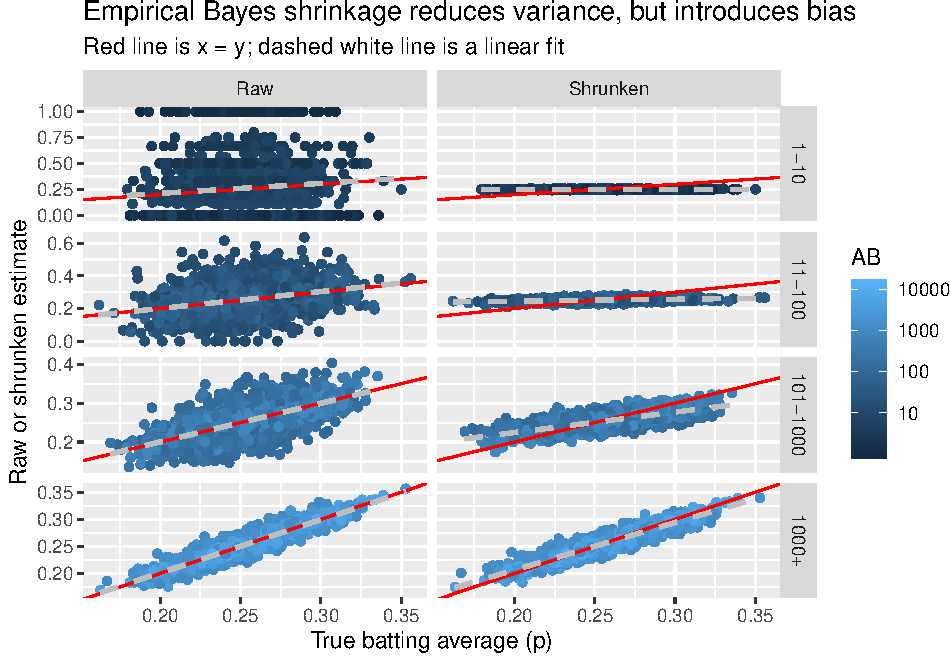
\includegraphics{datadown_files/figure-latex/simp-2.pdf}

\begin{itemize}
\tightlist
\item
  击球数越多,越接近真相
\end{itemize}

\hypertarget{ux533aux95f4ux4f30ux8ba1}{%
\subsection{区间估计}\label{ux533aux95f4ux4f30ux8ba1}}

\begin{itemize}
\tightlist
\item
  检验区间估计是否覆盖95\%的真值
\end{itemize}

\begin{Shaded}
\begin{Highlighting}[]
\NormalTok{career_sim_eb }\OperatorTok
\StringTok{  }\KeywordTok{summarize}\NormalTok{(}\DataTypeTok{coverage =} \KeywordTok{mean}\NormalTok{(.low }\OperatorTok{<=}\StringTok{ }\NormalTok{p }\OperatorTok{&}\StringTok{ }\NormalTok{p }\OperatorTok{<=}\StringTok{ }\NormalTok{.high))}
\end{Highlighting}
\end{Shaded}

\begin{verbatim}
## # A tibble: 1 x 1
##   coverage
##      <dbl>
## 1    0.945
\end{verbatim}

\begin{itemize}
\tightlist
\item
  观察不同区间的覆盖范围
\end{itemize}

\begin{Shaded}
\begin{Highlighting}[]
\NormalTok{sim_prior <-}\StringTok{ }\KeywordTok{ebb_fit_prior}\NormalTok{(career_sim, H, AB)}
\NormalTok{estimate_by_cred_level <-}\StringTok{ }\KeywordTok{data_frame}\NormalTok{(}\DataTypeTok{level =} \KeywordTok{seq}\NormalTok{(.}\DecValTok{5}\NormalTok{, }\FloatTok{.98}\NormalTok{, }\FloatTok{.02}\NormalTok{)) }\OperatorTok
\StringTok{  }\KeywordTok{mutate}\NormalTok{(}\DataTypeTok{model=}\KeywordTok{map}\NormalTok{(level, }\OperatorTok{~}\StringTok{ }\KeywordTok{augment}\NormalTok{(sim_prior, career_sim, }\DataTypeTok{cred_level =}\NormalTok{ .))) }\OperatorTok
\StringTok{  }\KeywordTok{unnest}\NormalTok{(model)}

\NormalTok{estimate_by_cred_level }\OperatorTok
\StringTok{  }\KeywordTok{group_by}\NormalTok{(level) }\OperatorTok
\StringTok{  }\KeywordTok{mutate}\NormalTok{(}\DataTypeTok{cover =}\NormalTok{ .low }\OperatorTok{<=}\StringTok{ }\NormalTok{p }\OperatorTok{&}\StringTok{ }\NormalTok{p }\OperatorTok{<=}\StringTok{ }\NormalTok{.high) }\OperatorTok
\StringTok{  }\KeywordTok{summarize}\NormalTok{(}\DataTypeTok{coverage =} \KeywordTok{mean}\NormalTok{(cover)) }\OperatorTok
\StringTok{  }\KeywordTok{ggplot}\NormalTok{(}\KeywordTok{aes}\NormalTok{(level, coverage)) }\OperatorTok{+}
\StringTok{  }\KeywordTok{geom_point}\NormalTok{() }\OperatorTok{+}
\StringTok{  }\KeywordTok{geom_abline}\NormalTok{(}\DataTypeTok{color =} \StringTok{"red"}\NormalTok{) }\OperatorTok{+}
\StringTok{  }\KeywordTok{labs}\NormalTok{(}\DataTypeTok{x =} \StringTok{"Level of credible interval"}\NormalTok{,}
       \DataTypeTok{y =} \StringTok{"Probability credible interval contains the true value"}\NormalTok{)}
\end{Highlighting}
\end{Shaded}

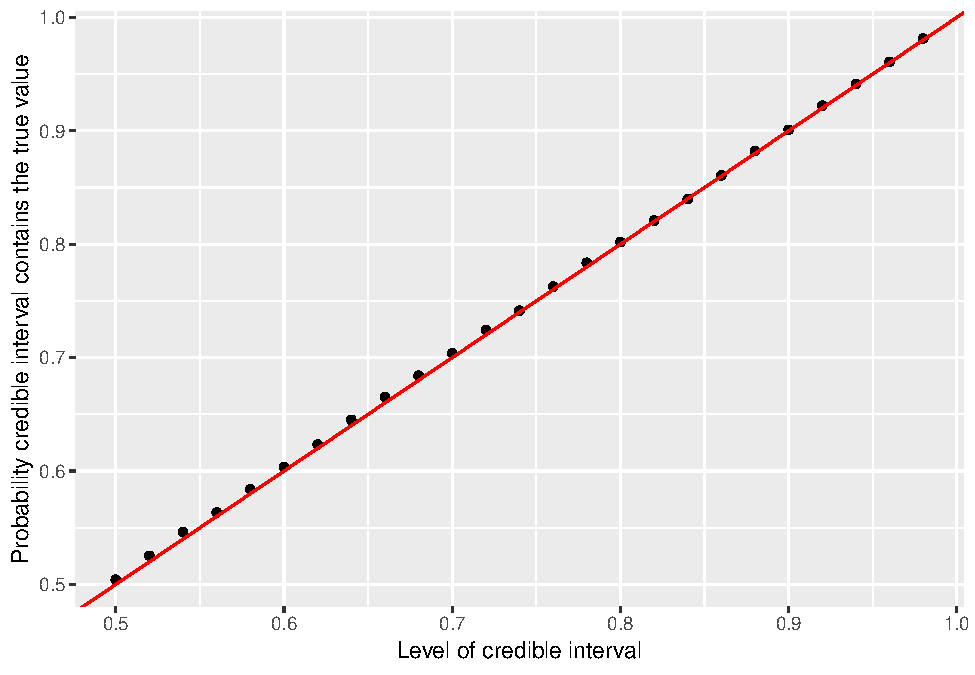
\includegraphics{datadown_files/figure-latex/simmint-1.pdf}

\begin{itemize}
\tightlist
\item
  结果基本吻合,说明区间估计也比较准
\end{itemize}

\hypertarget{ux9519ux8befux53d1ux73b0ux7387-1}{%
\subsection{错误发现率}\label{ux9519ux8befux53d1ux73b0ux7387-1}}

\begin{itemize}
\tightlist
\item
  看一下进入名人堂的人
\end{itemize}

\begin{Shaded}
\begin{Highlighting}[]
\NormalTok{pt <-}\StringTok{ }\NormalTok{career_sim_eb }\OperatorTok
\StringTok{  }\KeywordTok{add_ebb_prop_test}\NormalTok{(.}\DecValTok{3}\NormalTok{, }\DataTypeTok{sort =} \OtherTok{TRUE}\NormalTok{)}

\CommentTok{# 错误发现率控制为10%}
\NormalTok{hall_of_fame <-}\StringTok{ }\NormalTok{pt }\OperatorTok
\StringTok{  }\KeywordTok{filter}\NormalTok{(.qvalue }\OperatorTok{<=}\StringTok{ }\FloatTok{.1}\NormalTok{)}

\KeywordTok{mean}\NormalTok{(hall_of_fame}\OperatorTok{$}\NormalTok{p }\OperatorTok{<}\StringTok{ }\FloatTok{.3}\NormalTok{)}
\end{Highlighting}
\end{Shaded}

\begin{verbatim}
## [1] 0.157
\end{verbatim}

\begin{Shaded}
\begin{Highlighting}[]
\CommentTok{# 观察整体错误发现率的变动}
\NormalTok{pt }\OperatorTok
\StringTok{  }\KeywordTok{mutate}\NormalTok{(}\DataTypeTok{true_fdr =} \KeywordTok{cummean}\NormalTok{(p }\OperatorTok{<}\StringTok{ }\FloatTok{.3}\NormalTok{)) }\OperatorTok
\StringTok{  }\KeywordTok{ggplot}\NormalTok{(}\KeywordTok{aes}\NormalTok{(.qvalue, true_fdr)) }\OperatorTok{+}
\StringTok{  }\KeywordTok{geom_line}\NormalTok{() }\OperatorTok{+}
\StringTok{  }\KeywordTok{geom_abline}\NormalTok{(}\DataTypeTok{color =} \StringTok{"red"}\NormalTok{) }\OperatorTok{+}
\StringTok{  }\KeywordTok{labs}\NormalTok{(}\DataTypeTok{x =} \StringTok{"q-value"}\NormalTok{,}
       \DataTypeTok{y =} \StringTok{"True FDR at this q-value threshold"}\NormalTok{)}
\end{Highlighting}
\end{Shaded}

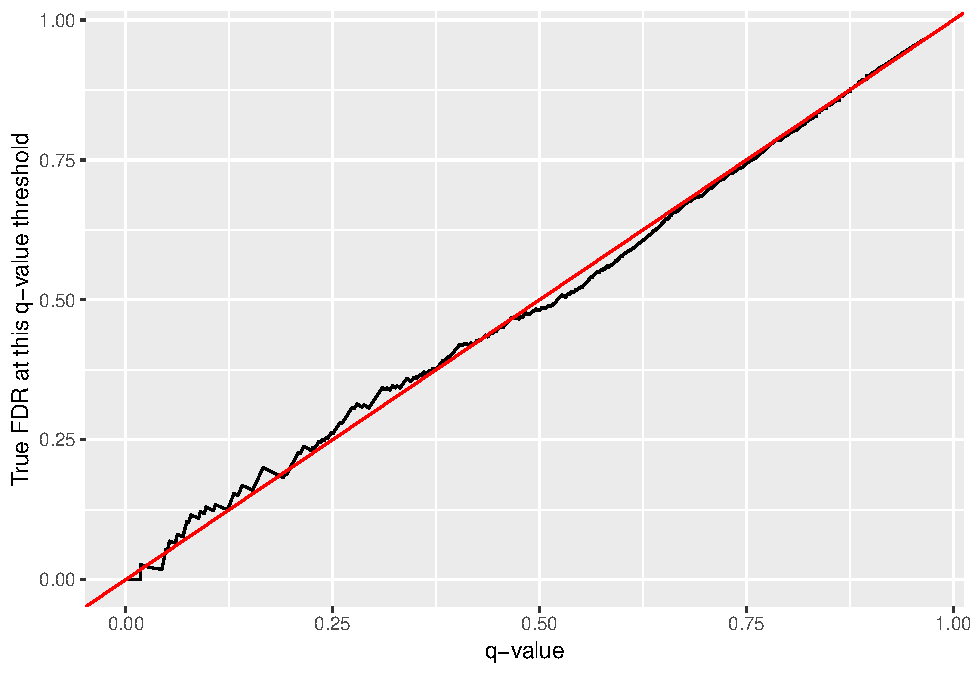
\includegraphics{datadown_files/figure-latex/simfdr-1.pdf}

\hypertarget{ux8d1dux5854ux4e8cux9879ux56deux5f52}{%
\subsection{贝塔二项回归}\label{ux8d1dux5854ux4e8cux9879ux56deux5f52}}

\begin{itemize}
\tightlist
\item
  看下影响因素
\end{itemize}

\begin{Shaded}
\begin{Highlighting}[]
\CommentTok{# 回归值}
\NormalTok{bb_reg <-}\StringTok{ }\NormalTok{career }\OperatorTok
\StringTok{  }\KeywordTok{ebb_fit_prior}\NormalTok{(H, AB, }\DataTypeTok{method =} \StringTok{"gamlss"}\NormalTok{, }\DataTypeTok{mu_predictors =} \OperatorTok{~}\StringTok{ }\KeywordTok{log10}\NormalTok{(AB))}

\KeywordTok{tidy}\NormalTok{(bb_reg)}
\end{Highlighting}
\end{Shaded}

\begin{verbatim}
## # A tibble: 3 x 6
##   parameter term        estimate std.error statistic p.value
##   <chr>     <chr>          <dbl>     <dbl>     <dbl>   <dbl>
## 1 mu        (Intercept)   -1.69    0.00885    -191.        0
## 2 mu        log10(AB)      0.192   0.00273      70.2       0
## 3 sigma     (Intercept)   -6.31    0.0227     -278.        0
\end{verbatim}

\begin{Shaded}
\begin{Highlighting}[]
\KeywordTok{set.seed}\NormalTok{(}\DecValTok{2017}\NormalTok{)}

\NormalTok{career_sim_ab <-}\StringTok{ }\KeywordTok{augment}\NormalTok{(bb_reg, career) }\OperatorTok
\StringTok{  }\NormalTok{dplyr}\OperatorTok{::}\KeywordTok{select}\NormalTok{(playerID, AB, }\DataTypeTok{true_alpha0 =}\NormalTok{ .alpha0, }\DataTypeTok{true_beta0 =}\NormalTok{ .beta0) }\OperatorTok
\StringTok{  }\KeywordTok{mutate}\NormalTok{(}\DataTypeTok{p =} \KeywordTok{rbeta}\NormalTok{(}\KeywordTok{n}\NormalTok{(), true_alpha0, true_beta0),}
         \DataTypeTok{H =} \KeywordTok{rbinom}\NormalTok{(}\KeywordTok{n}\NormalTok{(), AB, p))}
\CommentTok{# 真实值}
\NormalTok{career_ab_prior <-}\StringTok{ }\NormalTok{career_sim_ab }\OperatorTok
\StringTok{  }\KeywordTok{ebb_fit_prior}\NormalTok{(H, AB, }\DataTypeTok{method =} \StringTok{"gamlss"}\NormalTok{, }\DataTypeTok{mu_predictors =} \OperatorTok{~}\StringTok{ }\KeywordTok{log10}\NormalTok{(AB))}

\CommentTok{# 对比}
\KeywordTok{tidy}\NormalTok{(career_ab_prior)}
\end{Highlighting}
\end{Shaded}

\begin{verbatim}
## # A tibble: 3 x 6
##   parameter term        estimate std.error statistic p.value
##   <chr>     <chr>          <dbl>     <dbl>     <dbl>   <dbl>
## 1 mu        (Intercept)   -1.67    0.00880    -190.        0
## 2 mu        log10(AB)      0.187   0.00272      69.0       0
## 3 sigma     (Intercept)   -6.32    0.0267     -237.        0
\end{verbatim}

\begin{Shaded}
\begin{Highlighting}[]
\CommentTok{# 观察击球数影响}
\NormalTok{career_flat_prior <-}\StringTok{ }\NormalTok{career_sim_ab }\OperatorTok
\StringTok{  }\KeywordTok{ebb_fit_prior}\NormalTok{(H, AB)}

\KeywordTok{data_frame}\NormalTok{(}\DataTypeTok{method =} \KeywordTok{c}\NormalTok{(}\StringTok{"Flat prior"}\NormalTok{, }\StringTok{"Prior depending on AB"}\NormalTok{),}
           \DataTypeTok{model =} \KeywordTok{list}\NormalTok{(career_flat_prior, career_ab_prior)) }\OperatorTok
\StringTok{  }\KeywordTok{mutate}\NormalTok{(}\DataTypeTok{model=}\KeywordTok{map}\NormalTok{(model, augment, }\DataTypeTok{data =}\NormalTok{ career_sim_ab)) }\OperatorTok
\StringTok{  }\KeywordTok{unnest}\NormalTok{(model) }\OperatorTok
\StringTok{  }\KeywordTok{ggplot}\NormalTok{(}\KeywordTok{aes}\NormalTok{(p, .fitted, }\DataTypeTok{color =}\NormalTok{ AB)) }\OperatorTok{+}
\StringTok{  }\KeywordTok{geom_point}\NormalTok{() }\OperatorTok{+}
\StringTok{  }\KeywordTok{scale_color_continuous}\NormalTok{(}\DataTypeTok{trans =} \StringTok{"log"}\NormalTok{) }\OperatorTok{+}
\StringTok{  }\KeywordTok{geom_abline}\NormalTok{(}\DataTypeTok{color =} \StringTok{"red"}\NormalTok{) }\OperatorTok{+}
\StringTok{  }\KeywordTok{facet_wrap}\NormalTok{(}\OperatorTok{~}\StringTok{ }\NormalTok{method) }\OperatorTok{+}
\StringTok{  }\KeywordTok{labs}\NormalTok{(}\DataTypeTok{x =} \StringTok{"True batting average (p)"}\NormalTok{,}
       \DataTypeTok{y =} \StringTok{"Shrunken batting average estimate"}\NormalTok{)}
\end{Highlighting}
\end{Shaded}

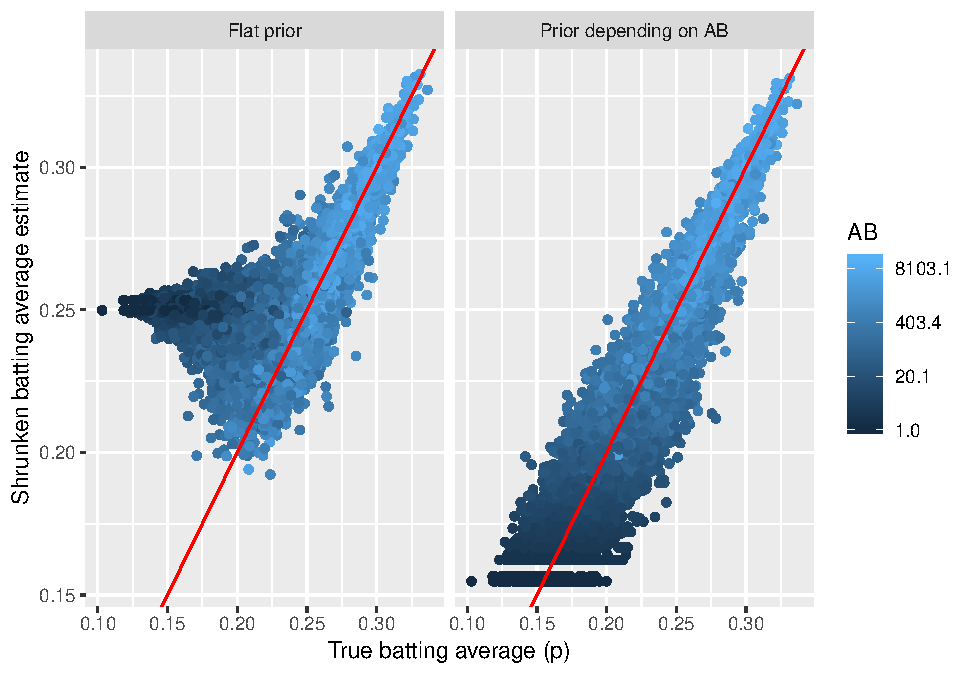
\includegraphics{datadown_files/figure-latex/simbbreg-1.pdf}

\hypertarget{ux91cdux590dux6a21ux62df}{%
\subsection{重复模拟}\label{ux91cdux590dux6a21ux62df}}

\begin{itemize}
\tightlist
\item
  为防止意外或运气可以重复模拟看看
\end{itemize}

\begin{Shaded}
\begin{Highlighting}[]
\KeywordTok{set.seed}\NormalTok{(}\DecValTok{2019}\NormalTok{)}

\NormalTok{sim_replications <-}\StringTok{ }\NormalTok{career }\OperatorTok
\StringTok{  }\KeywordTok{crossing}\NormalTok{(}\DataTypeTok{replication =} \DecValTok{1}\OperatorTok{:}\DecValTok{50}\NormalTok{) }\OperatorTok
\StringTok{  }\KeywordTok{mutate}\NormalTok{(}\DataTypeTok{p =} \KeywordTok{rbeta}\NormalTok{(}\KeywordTok{n}\NormalTok{(), alpha0, beta0),}
         \DataTypeTok{H =} \KeywordTok{rbinom}\NormalTok{(}\KeywordTok{n}\NormalTok{(), AB, p))}

\NormalTok{sim_replications}

\NormalTok{sim_replication_models <-}\StringTok{ }\NormalTok{sim_replications }\OperatorTok
\StringTok{  }\KeywordTok{nest}\NormalTok{(}\OperatorTok{-}\NormalTok{replication) }\OperatorTok
\StringTok{  }\KeywordTok{mutate}\NormalTok{(}\DataTypeTok{prior =}\NormalTok{ purrr}\OperatorTok{::}\KeywordTok{map}\NormalTok{(data, }\OperatorTok{~}\StringTok{ }\KeywordTok{ebb_fit_prior}\NormalTok{(., H, AB)))}

\CommentTok{# 估计参数}
\NormalTok{sim_replication_priors <-}\StringTok{ }\NormalTok{sim_replication_models }\OperatorTok
\StringTok{  }\KeywordTok{mutate}\NormalTok{(}\DataTypeTok{model=} \KeywordTok{map}\NormalTok{(prior, tidy)) }\OperatorTok
\StringTok{  }\NormalTok{dplyr}\OperatorTok{::}\KeywordTok{select}\NormalTok{(}\OperatorTok{-}\KeywordTok{c}\NormalTok{(data,prior)) }\OperatorTok
\StringTok{  }\KeywordTok{unnest}\NormalTok{(model)}

\NormalTok{sim_replication_priors}

\NormalTok{true_values <-}\StringTok{ }\KeywordTok{data_frame}\NormalTok{(}\DataTypeTok{parameter =} \KeywordTok{c}\NormalTok{(}\StringTok{"alpha"}\NormalTok{, }\StringTok{"beta"}\NormalTok{, }\StringTok{"mean"}\NormalTok{),}
                          \DataTypeTok{true =} \KeywordTok{c}\NormalTok{(alpha0, beta0, alpha0 }\OperatorTok{/}\StringTok{ }\NormalTok{(alpha0 }\OperatorTok{+}\StringTok{ }\NormalTok{beta0)))}

\NormalTok{sim_replication_priors }\OperatorTok
\StringTok{  }\KeywordTok{gather}\NormalTok{(parameter, value, }\OperatorTok{-}\NormalTok{replication) }\OperatorTok
\StringTok{  }\KeywordTok{inner_join}\NormalTok{(true_values, }\DataTypeTok{by =} \StringTok{"parameter"}\NormalTok{) }\OperatorTok
\StringTok{  }\KeywordTok{ggplot}\NormalTok{(}\KeywordTok{aes}\NormalTok{(}\DecValTok{1}\NormalTok{, value)) }\OperatorTok{+}
\StringTok{  }\KeywordTok{geom_boxplot}\NormalTok{() }\OperatorTok{+}
\StringTok{  }\KeywordTok{geom_hline}\NormalTok{(}\KeywordTok{aes}\NormalTok{(}\DataTypeTok{yintercept =}\NormalTok{ true), }\DataTypeTok{color =} \StringTok{"red"}\NormalTok{, }\DataTypeTok{lty =} \DecValTok{2}\NormalTok{) }\OperatorTok{+}
\StringTok{  }\KeywordTok{facet_wrap}\NormalTok{(}\OperatorTok{~}\StringTok{ }\NormalTok{parameter, }\DataTypeTok{scales =} \StringTok{"free_y"}\NormalTok{) }\OperatorTok{+}
\StringTok{  }\KeywordTok{labs}\NormalTok{(}\DataTypeTok{x =} \StringTok{""}\NormalTok{,}
       \DataTypeTok{y =} \StringTok{"Estimated parameter (true value shown as red line)"}\NormalTok{,}
       \DataTypeTok{title =} \StringTok{"Estimated hyperparameters across 50 replications"}\NormalTok{)}

\CommentTok{# 估计区间与假设检验}

\CommentTok{## 估计均方误}
\NormalTok{sim_replication_au <-}\StringTok{ }\NormalTok{sim_replication_models }\OperatorTok
\StringTok{  }\KeywordTok{mutate}\NormalTok{(}\DataTypeTok{model=}\KeywordTok{map2}\NormalTok{(prior, data, augment)) }\OperatorTok
\StringTok{  }\KeywordTok{unnest}\NormalTok{(model)}

\NormalTok{sim_replication_mse <-}\StringTok{ }\NormalTok{sim_replication_au }\OperatorTok
\StringTok{  }\KeywordTok{rename}\NormalTok{(}\DataTypeTok{Raw =}\NormalTok{ .raw, }\DataTypeTok{Shrunken =}\NormalTok{ .fitted) }\OperatorTok
\StringTok{  }\KeywordTok{gather}\NormalTok{(type, estimate, Raw, Shrunken) }\OperatorTok
\StringTok{  }\KeywordTok{group_by}\NormalTok{(type, replication) }\OperatorTok
\StringTok{  }\KeywordTok{summarize}\NormalTok{(}\DataTypeTok{mse =} \KeywordTok{mean}\NormalTok{((estimate }\OperatorTok{-}\StringTok{ }\NormalTok{p) }\OperatorTok{^}\StringTok{ }\DecValTok{2}\NormalTok{))}

\KeywordTok{ggplot}\NormalTok{(sim_replication_mse, }\KeywordTok{aes}\NormalTok{(type, mse)) }\OperatorTok{+}
\StringTok{  }\KeywordTok{geom_boxplot}\NormalTok{() }\OperatorTok{+}
\StringTok{  }\KeywordTok{ylab}\NormalTok{(}\StringTok{"Mean squared error across 50 replications"}\NormalTok{)}
\CommentTok{## 估计区间}
\NormalTok{sim_replication_au }\OperatorTok
\StringTok{  }\KeywordTok{mutate}\NormalTok{(}\DataTypeTok{cover =}\NormalTok{ .low }\OperatorTok{<=}\StringTok{ }\NormalTok{p }\OperatorTok{&}\StringTok{ }\NormalTok{p }\OperatorTok{<=}\StringTok{ }\NormalTok{.high) }\OperatorTok
\StringTok{  }\KeywordTok{group_by}\NormalTok{(replication) }\OperatorTok
\StringTok{  }\KeywordTok{summarize}\NormalTok{(}\DataTypeTok{coverage =} \KeywordTok{mean}\NormalTok{(cover)) }\OperatorTok
\StringTok{  }\KeywordTok{ggplot}\NormalTok{(}\KeywordTok{aes}\NormalTok{(coverage)) }\OperatorTok{+}
\StringTok{  }\KeywordTok{geom_histogram}\NormalTok{(}\DataTypeTok{binwidth =} \FloatTok{.001}\NormalTok{) }\OperatorTok{+}
\StringTok{  }\KeywordTok{labs}\NormalTok{(}\DataTypeTok{x =} \StringTok{"% of time true value was in a 95% confidence interval"}\NormalTok{,}
       \DataTypeTok{title =} \StringTok{"95% credible interval is well calibrated across replications"}\NormalTok{)}

\NormalTok{sim_replication_intervals <-}\StringTok{ }\NormalTok{sim_replication_models }\OperatorTok
\StringTok{  }\KeywordTok{expand_grid}\NormalTok{(}\DataTypeTok{cred_level =} \KeywordTok{c}\NormalTok{(}\KeywordTok{seq}\NormalTok{(.}\DecValTok{5}\NormalTok{, }\FloatTok{.9}\NormalTok{, }\FloatTok{.05}\NormalTok{), }\FloatTok{.95}\NormalTok{)) }\OperatorTok
\StringTok{  }\KeywordTok{mutate}\NormalTok{(}\DataTypeTok{model=}\KeywordTok{pmap}\NormalTok{(}\KeywordTok{list}\NormalTok{(prior, data, }\DataTypeTok{cred_level =}\NormalTok{ cred_level), augment)) }\OperatorTok
\StringTok{  }\KeywordTok{unnest}\NormalTok{(model) }\OperatorTok
\StringTok{  }\NormalTok{dplyr}\OperatorTok{::}\KeywordTok{select}\NormalTok{(replication, cred_level, p, .low, .high)}

\NormalTok{sim_replication_intervals }\OperatorTok
\StringTok{  }\KeywordTok{mutate}\NormalTok{(}\DataTypeTok{cover =}\NormalTok{ .low }\OperatorTok{<=}\StringTok{ }\NormalTok{p }\OperatorTok{&}\StringTok{ }\NormalTok{p }\OperatorTok{<=}\StringTok{ }\NormalTok{.high) }\OperatorTok
\StringTok{  }\KeywordTok{group_by}\NormalTok{(replication, cred_level) }\OperatorTok
\StringTok{  }\KeywordTok{summarize}\NormalTok{(}\DataTypeTok{coverage =} \KeywordTok{mean}\NormalTok{(cover)) }\OperatorTok
\StringTok{  }\KeywordTok{ggplot}\NormalTok{(}\KeywordTok{aes}\NormalTok{(cred_level, coverage, }\DataTypeTok{group =}\NormalTok{ replication)) }\OperatorTok{+}
\StringTok{  }\KeywordTok{geom_line}\NormalTok{(}\DataTypeTok{alpha =} \FloatTok{.3}\NormalTok{) }\OperatorTok{+}
\StringTok{  }\KeywordTok{geom_abline}\NormalTok{(}\DataTypeTok{color =} \StringTok{"red"}\NormalTok{) }\OperatorTok{+}
\StringTok{  }\KeywordTok{labs}\NormalTok{(}\DataTypeTok{x =} \StringTok{"Credibility level"}\NormalTok{,}
       \DataTypeTok{y =} \StringTok{"% of credible intervals in this replication that contain the true parameter"}\NormalTok{,}
       \DataTypeTok{title =} \StringTok{"Credible intervals are well calibrated across 50 replications"}\NormalTok{,}
       \DataTypeTok{subtitle =} \StringTok{"Red line is x = y"}\NormalTok{)}

\CommentTok{# q值的稳定性}

\NormalTok{sim_replication_prop_tests <-}\StringTok{ }\NormalTok{sim_replication_au }\OperatorTok
\StringTok{   }\KeywordTok{nest}\NormalTok{(}\OperatorTok{-}\NormalTok{replication) }\OperatorTok
\StringTok{   }\KeywordTok{mutate}\NormalTok{(}\DataTypeTok{model=}\KeywordTok{map}\NormalTok{(data, add_ebb_prop_test, }\DataTypeTok{threshold =} \FloatTok{.3}\NormalTok{, }\DataTypeTok{sort =} \OtherTok{TRUE}\NormalTok{)) }\OperatorTok
\StringTok{   }\KeywordTok{unnest}\NormalTok{(model)}

\NormalTok{sim_replication_prop_tests }\OperatorTok
\StringTok{   }\KeywordTok{group_by}\NormalTok{(replication) }\OperatorTok
\StringTok{   }\KeywordTok{mutate}\NormalTok{(}\DataTypeTok{fdr =} \KeywordTok{cummean}\NormalTok{(p }\OperatorTok{<}\StringTok{ }\FloatTok{.3}\NormalTok{)) }\OperatorTok
\StringTok{   }\KeywordTok{ggplot}\NormalTok{(}\KeywordTok{aes}\NormalTok{(.qvalue, fdr, }\DataTypeTok{group =}\NormalTok{ replication)) }\OperatorTok{+}
\StringTok{   }\KeywordTok{geom_line}\NormalTok{(}\DataTypeTok{alpha =} \FloatTok{.3}\NormalTok{) }\OperatorTok{+}
\StringTok{   }\KeywordTok{geom_abline}\NormalTok{(}\DataTypeTok{color =} \StringTok{"red"}\NormalTok{) }\OperatorTok{+}
\StringTok{   }\KeywordTok{labs}\NormalTok{(}\DataTypeTok{x =} \StringTok{"Q-value threshold"}\NormalTok{,}
        \DataTypeTok{y =} \StringTok{"Proportion of false discoveries below this threshold"}\NormalTok{,}
        \DataTypeTok{title =} \StringTok{"Q-value successfully controls FDR across 50 replications"}\NormalTok{)}
\end{Highlighting}
\end{Shaded}

\hypertarget{bayeslink}{%
\section{网络资源}\label{bayeslink}}

\begin{itemize}
\tightlist
\item
  \href{http://mindhacks.cn/2008/09/21/the-magical-bayesian-method/}{贝叶斯方法}
\item
  \href{https://github.com/mavelli/rocker-bayesian}{贝叶斯镜像}
\end{itemize}

\hypertarget{why}{%
\chapter{因果分析}\label{why}}

\hypertarget{introduction}{%
\section{Introduction}\label{introduction}}

\begin{quote}
``Impact assessment, simply defined, is the process of identifying the future consequences of a current or proposed action.'' (IAIA, 2009)
\end{quote}

\begin{quote}
``Policy assessment seeks to inform decision-makers by predicting and evaluating the potential impacts of policy options.'' (Adelle and Weiland, 2012)
\end{quote}

\begin{quote}
``\ldots{} I see no greater impediment to scientific progress than the prevailing practice of focusing all our mathematical resources on probabilistic and statistical inferences while leaving causal considerations to the mercy of intuition and good judgment.'' (Pearl, 1999)
\end{quote}

\hypertarget{causal-information}{%
\section{Causal Information}\label{causal-information}}

\hypertarget{target}{%
\subsection{Target}\label{target}}

\begin{quote}
practical framework for causal effect estimation in the context of policy assessment and impact analysis, and in the absence of experimental data
\end{quote}

\hypertarget{causal-sources}{%
\subsection{Causal sources}\label{causal-sources}}

\begin{itemize}
\tightlist
\item
  Causal Inference by Experiment: Randomized experiments
\item
  Causal Inference from Observational Data and Theory: Existing data or Big data
\end{itemize}

\hypertarget{identification-and-estimation-process}{%
\subsection{Identification and Estimation Process}\label{identification-and-estimation-process}}

\begin{itemize}
\tightlist
\item
  Causal Identification: domain knowledge based
\item
  Computing the Effect Size: Bayesian networks
\end{itemize}

\hypertarget{theoretical-background}{%
\section{Theoretical Background}\label{theoretical-background}}

\hypertarget{potential-outcomes-framework}{%
\subsection{Potential Outcomes Framework}\label{potential-outcomes-framework}}

\begin{itemize}
\tightlist
\item
  \(Y_{i,1}\) Potential outcome of individual i given treatment T=1 (e.g.~taking two Aspirins)
\item
  \(Y_{i,0}\) Potential outcome of individual i given treatment T=0 (e.g.~drinking a glass of water)
\item
  individual-level causal effect (ICE)

  \begin{itemize}
  \tightlist
  \item
    \(ICE=Y_{i,1} −Y_{i,0}\)
  \end{itemize}
\item
  average causal effect (ACE)

  \begin{itemize}
  \tightlist
  \item
    \(ACE = E[Y_{i,1}] −E[Y_{i,0}]\)
  \end{itemize}
\end{itemize}

\hypertarget{causal-identification}{%
\subsection{Causal Identification}\label{causal-identification}}

\begin{itemize}
\tightlist
\item
  \(Y_{i,1}\) (treatment) and \(Y_{i,0}\) (non-treatment) can never be both observed for the same individual at the same time
\item
  Association S

  \begin{itemize}
  \tightlist
  \item
    \(S = E[Y_1|T = 1] - E[Y_0|T = 0]\)
  \end{itemize}
\item
  S is not the \textbf{same} with ACE

  \begin{itemize}
  \tightlist
  \item
    association does not imply causation
  \item
    randomized experiment
  \end{itemize}
\end{itemize}

\hypertarget{ignorability}{%
\subsubsection{Ignorability}\label{ignorability}}

\begin{itemize}
\tightlist
\item
  \((Y_1,Y_0) \upmodels T\), \(Y_1\) and \(Y_0\) must be jointly independent of the treatment assignment
\item
  \((Y_1,Y_0) \upmodels T|X\) for realobservational studies, conditional on variables X, \(Y_1\), and \(Y_0\) are jointly independent of T, the assignment mechanism
\item
  \(ACE|X = E[Y_1|X] - E[Y_0|X] = E[Y_1|T=1,X] - E[Y_0|􏰀T = 0,X] = E[Y|􏰀T = 1,X] - E[Y|􏰀T =0,X] = S|􏰀X\)
\end{itemize}

\hypertarget{assumptions}{%
\subsubsection{Assumptions}\label{assumptions}}

\begin{itemize}
\tightlist
\item
  Causal inference requires causal assumptions
\end{itemize}

\hypertarget{methods-for-identification-and-estimation}{%
\section{Methods for Identification and Estimation}\label{methods-for-identification-and-estimation}}

\hypertarget{directed-acyclic-graphsdag-for-identification}{%
\subsection{Directed Acyclic Graphs(DAG) for Identification}\label{directed-acyclic-graphsdag-for-identification}}

\begin{itemize}
\tightlist
\item
  DAGs Are Nonparametric
\item
  A Node represents a variable in a domain, regardless of whether it is observable or unobservable
\item
  A Directed Arc has the appearance of an arrow and represents a potential causal effect. The arc direction indicates the assumed causal direction, i.e. ``A→B'' means ``A causes B.''
\item
  A Missing Arc encodes the definitive absence of a direct causal effect, i.e.~no arc between A and B means that there exists no direct causal relationship between A and B and vice versa. As such, a missing arc repre- sents an assumption
\end{itemize}

\hypertarget{indirect-connection}{%
\subsection{Indirect Connection}\label{indirect-connection}}

\begin{itemize}
\tightlist
\item
  A causes B via node C
\item
  \(A \nupmodels B\) and \(A \upmodels B|C\)
\end{itemize}

\hypertarget{common-cause}{%
\subsection{Common Cause}\label{common-cause}}

\begin{itemize}
\tightlist
\item
  C causes both A and B
\item
  \(A \nupmodels B\) and \(A \upmodels B|C\)
\end{itemize}

\hypertarget{common-effect}{%
\subsection{Common Effect}\label{common-effect}}

\begin{itemize}
\tightlist
\item
  C is the common effect of A and B
\item
  \(A \upmodels B\) and \(A \nupmodels B|C\)
\end{itemize}

\hypertarget{example-simpsons-paradox}{%
\subsection{Example: Simpson's Paradox}\label{example-simpsons-paradox}}

\hypertarget{yinguolink}{%
\section{链接}\label{yinguolink}}

\begin{itemize}
\tightlist
\item
  \href{https://cosx.org/2012/03/causality1-simpson-paradox}{因果推断}
\item
  \href{https://github.com/google/CausalImpact}{Google的因果分析包}
\end{itemize}

\hypertarget{neta}{%
\chapter{网络分析}\label{neta}}

\hypertarget{ux56feux8bba}{%
\section{图论}\label{ux56feux8bba}}

\begin{itemize}
\tightlist
\item
  最早是七桥问题
\item
  网络里节点(node)与连接(link)对应图论里的交点(vertex)与边(edge)
\item
  (N,L)表示一个系统
\item
  节点的度指的是节点对内对外的连接数
\item
  网络的度指的是所有节点的平均度,无方向的除2
\item
  均值 \(<x^n> = \frac{x_1^n+x_2^n+...+x_N^n}{N} = \frac{1}{N}\sum_{i=1}^N x_i^n\)
\item
  方差 \(\sigma_x = \sqrt{\frac{1}{N}\sum_{i=1}^N (x_i-<x>)^2}\)
\item
  度的概率分布 \(p_x = \frac{1}{N}\sum_i \delta_{x,x_i}\) \(\sum_ip_x = 1\)
\item
  连接矩阵 \(A_{ij}\) \(A_{ij} = 1\) 表示点有链接 无方向的上下矩阵对称
\item
  连接矩阵通常是稀疏的
\item
  全连接网络 \(L_{max} = \frac{N(N-1)}{2}\) 平均度 \(<k> = N-1\)
\item
  二分图,顶点可分成互斥独立集U和V
\item
  聚集系数,邻居互相连接的比例 \(C_i = \frac{2e_i}{k_i(k_i-1)}\) \(C_i =1\) 表示全连接,0表示全不连接
\end{itemize}

\hypertarget{ux968fux673aux7f51ux7edcux6a21ux578b}{%
\section{随机网络模型}\label{ux968fux673aux7f51ux7edcux6a21ux578b}}

\begin{itemize}
\tightlist
\item
  任意两点链接概率固定,符合二项分布的概率,度取决于概率与节点数
\item
  稀疏网络近似符合泊松分布,参数只有平均度
\item
  100点之下还是用二项分布
\item
  度是泊松分布
\item
  随机网络里出现高度节点的概率很低,与现实不符
\item
  平均度为1,也就是概率为\(\frac{1}{N}\)时,随机网络可出现大节点。小于1时网络高度节点的增长赶不上节点数增长。到了1时出现临界点,大的节点大概是 \(N^{\frac{2}{3}}\) 。当平均度达到 \(lnN(p>lnN/N)\) 时,所有节点连接在一起。
\item
  真实世界里平均度大于1小于\(lnN\),也就是存在大节点,但并不完全贯通,处于亚临界与全联通之间,为超临界状态
\item
  随机网络里节点数固定,单总距离数 \(N(d)\approx 1+<k>+<k>^2+...+<k>^d = \frac{<k>^{d+1}-1}{<k>-1}\)
\item
  最大距离 \(N(d_{max})\approx N \approx <k>^{d_{max}}\) 距离 \(d_{max} \approx\frac{lnN}{ln<k>}\)
\item
  网络连接越密集,平均距离越短
\item
  互联网平均距离 \(<d> \approx 0.35+0.89lnN\)
\item
  小世界特性,随机网络里平均距离比较短
\item
  聚集系数,邻居互相连接的比例 \(C_i = \frac{2<L_i>}{k_i(k_i-1)} = p = \frac{<k>}{N}\)
\item
  Watts-Strogatz 小世界模型,低平均距离与高聚集系数,处于完全聚集长距离的正则网络与不聚集短距离的随机网络之间
\end{itemize}

\hypertarget{ux65e0ux5c3aux5ea6ux7f51ux7edc}{%
\section{无尺度网络}\label{ux65e0ux5c3aux5ea6ux7f51ux7edc}}

\begin{itemize}
\tightlist
\item
  度的概率分布事符合幂律的 \(log p_k = -\gamma logCk+b\) ,其中\(\gamma\)是度指数
\item
  因为 \(\sum_{k=1}^\infty p_k = 1\),所以 \(C = \frac{1}{\sum_{k=1}^{\infty}k^{-\gamma}} = \frac{1}{\zeta(\gamma)}\)
\item
  后面那个是 Riemann-zeta 函数,因此概率 \(p_k = \frac{k^{-\gamma}}{\zeta(\gamma)}\)
\item
  最大的度 \(k_{max} = k_{min}N^{\frac{1}{\gamma -1}}\) 节点数越多,最大节点数越大,比随机网络大很多
\item
  无尺度主要是说n阶矩的分布 \(<k^n> = C\frac{k_{max}^{n-\gamma+1} - k_{min}^{n-\gamma+1}}{n-\gamma+1}\) ,多数无尺度网络的 \(\gamma\) 在2-3之间,因此除了一阶矩以外,所有的高阶矩都会非常大,随机网络则有尺度
\item
  超小特性,平均距离要比随机网络小很多,\(\gamma =2\) 平均距离是常数,2-3之间为\(lnlnN\),3为\(\frac{lnN}{lnlnN}\),大于3为\(lnN\)(小世界网络)。在无尺度网络里大节点会缩小距离。
\end{itemize}

\hypertarget{ux65e0ux5c3aux5ea6ux7684ux751fux6210---barabuxe1si-albert-ux6a21ux578b}{%
\section{无尺度的生成 - Barabási-Albert 模型}\label{ux65e0ux5c3aux5ea6ux7684ux751fux6210---barabuxe1si-albert-ux6a21ux578b}}

\begin{itemize}
\tightlist
\item
  网络的生长存在选择性依附,新节点会依附在度更高的节点上
\item
  生长概率 \(\prod (K_i) = \frac{k_i}{\sum_jk_j}\)
\item
  度动力学 \(\frac{dk_i}{dt} = m\prod(k_i) = m\frac{k_i}{\sum_{j=1}^{N-1}k_j}\)
\item
  m个连接 \(\sum_{j=1}^{N-1}k_j = 2mt-m\)
\item
  整理后得到 \(k_i(t) = m(\frac{t}{t_i})^{\beta}\),\(\beta\) 为0.5
\end{itemize}

\hypertarget{ux7f51ux7edcux7684ux8fdbux5316---bianconi-barabuxe1si-ux6a21ux578b}{%
\section{网络的进化 - Bianconi-Barabási 模型}\label{ux7f51ux7edcux7684ux8fdbux5316---bianconi-barabuxe1si-ux6a21ux578b}}

\begin{itemize}
\tightlist
\item
  选择依附会导致后来的成为节点概率低,无法解释现实世界里后来居上的现象
\item
  生长概率\(\prod (K_i) = \frac{\eta_ik_i}{\sum_j\eta_i k_j}\) \(\eta\) 代表适应度(fitness)
\item
  后来者适应度如果高,其度也很超过先来的
\item
  互联网适应度与概率指数分布,期刊适应度峰分布
\item
  物理机制可对应 波色-爱因斯坦凝聚态,适应度对应能量,新节点对应能级上新粒子,节点度对应能级上的粒子数。波色-爱因斯坦凝聚态可以无限吸引新粒子,因此不再无尺度,出现强者恒强
\item
  还要考虑节点删除与老化
\end{itemize}

\hypertarget{ux5ea6ux76f8ux5173}{%
\section{度相关}\label{ux5ea6ux76f8ux5173}}

\begin{itemize}
\item
  大节点似乎不连接大节点,小节点总是连接小节点
\item
  两个节点连接概率 \(p_{k,k'} = \frac{kk'}{2L}\)
\item
  神经网络是随机连接,符合概率
\item
  匹配性网络(assortative network),大节点互相连接,小节点只连接小节点,光环效应
\item
  非匹配性网络(disassortative network),大节点连接小节点但互相不连接
\item
  度相关矩阵 \(e_{ij}\)且\(\sum_{i,j}e_{ij} = 1\)
\item
  度的概率 \(q_k = \frac{kp_k}{<k>}\),因此 \(\sum_je_{ij} = q_i\)
\item
  单一节点度相关性 \(k_{nn}(k_i) = \frac{1}{k_i}\sum_{j=1}^NA_{ij}k_j\)
\item
  网络总相关性 \(k_{nn}(k) = \sum_{k'}k'P(k'|k)\)
\item
  神经网络里 \(k_{nn}(k)=\frac{<k^2>}{k}\)
\item
  近似公式 \(k_{nn}(k)=ak^{\mu}\)
\item
  神经网络 \(\mu = 0\),匹配性网络科学家合作网络 \(\mu>0\),非匹配性网络代谢网络 \(\mu<0\)
\item
  度相关系数 \(r=\sum_{jk}\frac{jk(e_{jk}-q_{j}q_{k})}{\sigma^2}\),其中\(\sigma^2=\sum_{k}k^2q_k - [\sum_kkq_k]^2\)
\item
  度相关系数\(r\)与相关指数\(\mu\)假设不同但基本相关
\item
  朋友悖论:朋友总比你受欢迎
\item
  真实网络存在度相关,改变度相关会改变网络性质,对网络功能的进一步描述
\item
  模型生成的配置模型与隐参数模型可根据度来生成模型
\item
  静态生成模型是非匹配或随机网络
\item
  当\(\gamma>3\),动态生成模型可能是弱匹配网络
\end{itemize}

\hypertarget{ux7f51ux7edcux7a33ux5065ux6027}{%
\section{网络稳健性}\label{ux7f51ux7edcux7a33ux5065ux6027}}

\begin{itemize}
\tightlist
\item
  去掉节点后网络功能性的影响,复原能力与冗余机制是稳健性保障
\item
  渗透理论(percolation),少量节点去除后不影响整体,但超过关键点后会碎裂成小集群,林火理论
\item
  Malloy-Reed 法则:\(\frac{<k^2>}{k}>2\) 判断是否存在大组分
\item
  随机错误 \(f_c = 1-\frac{1}{\frac{<k^2>}{<k>}-1}\)
\item
  随机网络 \(f_c^{ER}=1-\frac{1}{<k>}\) 无尺度网络二阶矩很大,所以容错高
\item
  提高稳健性 \(f_c>f_c^{ER}\)
\item
  遭受攻击时 \(f_c^{\frac{2-\gamma}{1-\gamma}}=2+\frac{2-\gamma}{1-\gamma}k_{min}(f_c^{\frac{3-\gamma}{1-\gamma}}-1)\)
\item
  如果优先攻击高度节点,那么稳健性会很低,随机进攻影响不大
\item
  攻击会造成级联反应,最稳健的网络一个中心节点,其余节点度相同,非无尺度网络
\item
  拉萨路效应(Lazarus effect):一个突变细菌继续敲除基因后会死而复生,继续繁殖,相当于林火模型里放任小火堆
\end{itemize}

\hypertarget{ux7f51ux7edcux96c6ux7fa4}{%
\section{网络集群}\label{ux7f51ux7edcux96c6ux7fa4}}

\begin{itemize}
\tightlist
\item
  假设1:集群存在与节点的连接关系中
\item
  假设2:集群内部联通度高
\item
  假设3:随机网络里没有集群
\item
  假设4:最大模块假设 \(M=\sum_{c=1}^{n_c}[\frac{l_c}{L}-(\frac{k_c}{2L})^2]\)
\item
  集群是否存在无法验证,所以只有假设
\item
  集群存在共享节点
\item
  算法很多, Louvain 与 the Infomap 比较快(\(o(NlogN)\)),cfinder 比较慢(\(o(e^N)\))
\item
  集群也存在生成与进化问题
\end{itemize}

\hypertarget{game}{%
\chapter{博弈论}\label{game}}

\hypertarget{ux672fux8bed-1}{%
\section{术语}\label{ux672fux8bed-1}}

\begin{itemize}
\tightlist
\item
  博弈论说白了就是讲两方势力在一件事上为了自己的最大利益所采取的行动或决策的理论
\item
  参与者(players) \(N= {1,...,n}\)
\item
  参与者 \(i\) 有一组行动(Actions),行动的集合 \(a=(a_1,...,a_n) \in A=A_1 \times A_2 \times ... \times A_n\)
\item
  参与者 \(i\) 的每个行为的收益(Payoffs)都可以用 \(u_i:A \rightarrow \Re\) 这个函数表示 \(u_i(a)\) 表示某个行为产生的收益,\(u = (u_i,...,u_n)\)是效用函数的集合
\item
  n个参与者的标准博弈(normal form) \(\langle N,A,u \rangle\)
\item
  两人博弈可以用矩阵(matrix)来描述,行代表选手1,列代表选手2,行对应选手1的行动 \(a_1 \in A_1\),列对应选手2的行动 \(a_2 \in A_2\),每个单元列出每个参与者的收益,先行选手,后列选手
\item
  纯竞争博弈(Games of Pure competition):两个参与者收益对立且对于所有行动集合 \(a \in A, u_1(a)+u_2(a) = c\),\(c\)是常数,零和博弈是一个常数为0的纯竞争博弈,此时我们只用考虑一个参与者的收益函数就可以了
\end{itemize}

\hypertarget{ux652fux914dux7b56ux7565dominate-strategy}{%
\section{支配策略(dominate strategy)}\label{ux652fux914dux7b56ux7565dominate-strategy}}

\begin{itemize}
\tightlist
\item
  行动单一称为纯策略(pure strategies)有一定概率分布的行动策略称为混合策略(mixed strategies)
\item
  对于一个参与者,不论其它参与者采取任何策略,某策略都会得到最大的收益
\item
  \(a_i \in a_i\) 为强支配策略当且仅当参与者\(i\) 的收益 \(u_i(a_i,a_{-i}) > u_i(a'_i,a_{-i})\),如果 \(a'_i = a_i\),那么为弱支配策略
\end{itemize}

\hypertarget{ux6700ux4f73ux56deux5e94best-respinse}{%
\section{最佳回应(Best respinse)}\label{ux6700ux4f73ux56deux5e94best-respinse}}

\begin{itemize}
\tightlist
\item
  对于一个参与者,当已知其他参与者的行为后,收益最大的策略
\item
  参与者\(i\),对于其它参与者的策略\(a_{-i} \in a_{-i}\) 的策略如果\(u_i(a_i,a_{-i}) \geqslant u_i(a'_i,a_{-i})\)
\end{itemize}

\hypertarget{ux7eb3ux4ec0ux5747ux8861nash-equilibrium}{%
\section{纳什均衡(Nash Equilibrium)}\label{ux7eb3ux4ec0ux5747ux8861nash-equilibrium}}

\begin{itemize}
\tightlist
\item
  \(a = \langle a_1,...,a_n\rangle\) 是一个纯策略纳什均衡当且仅当对于任何一个行为i,有\(a_i \in BR(a_{-i})\)
\item
  如果任何参与者改变行为的收益都不会增加,那么此时进入纳什均衡
\item
  纳什均衡是一系列行为的列表,这些行为都是稳定的
\item
  支配策略是纳什均衡但反过来不一定对
\item
  任何有限博弈都存在一个纳什均衡(纳什1950年提出)
\end{itemize}

\hypertarget{ux5e15ux7d2fux6258ux6700ux4f18pareto-optimality}{%
\section{帕累托最优(Pareto Optimality)}\label{ux5e15ux7d2fux6258ux6700ux4f18pareto-optimality}}

\begin{itemize}
\tightlist
\item
  某个结果是帕累托最优当且仅当没有其他结果可以全局帕累托支配这个结果
\item
  帕累托最优表示某个博弈结果不差于其他博弈结果
\item
  纳什均衡不一定是帕累托最优(囚徒困境)
\end{itemize}

\hypertarget{ux6df7ux5408ux7b56ux7565mixed-stratergies}{%
\section{混合策略(Mixed stratergies)}\label{ux6df7ux5408ux7b56ux7565mixed-stratergies}}

\begin{itemize}
\tightlist
\item
  策略\(S_i\)指对于每个参与者行动的概率分布集合
\item
  概率 \(Pr(a|s) = \prod_{j \in N}s_j(a_j)\)
\item
  期望收益函数 \(u_i(s) = \sum_{a \in A} u_i(a)Pr(a|s)\)
\item
  随机策略会使对手混乱进入动态,很多博弈只存在混合策略纳什均衡而没有纯策略纳什均衡(石头剪子布)
\item
  混合策略的目的在于不论你使用哪一种行动,对方的收益都不变
\end{itemize}

\begin{longtable}[]{@{}lll@{}}
\toprule
选手 & 甲 & 乙\tabularnewline
\midrule
\endhead
丙 & a,b & c,d\tabularnewline
丁 & e,f & g,h\tabularnewline
\bottomrule
\end{longtable}

\begin{itemize}
\tightlist
\item
  对于选手1而言,采取丙行动的收益是\(aq+c(1-q)\),采取丁行动的收益是\(eq+g(1-q)\),q代表选手2采取甲行动概率
\item
  如果要达到双方均衡,那么不论采取什么行动收益应该一致,不会因为对方概率的变化而偏离,那么我们就可以求解均衡时选手2的行动概率:
\end{itemize}

\[aq+c(1-q) = eq+g(1-q)\]

\[q = \frac{g-c}{a+g-c-e}\]

\begin{itemize}
\tightlist
\item
  这个结果表明选手2采取行动主要要参考选手1的行动收益差
\item
  同理,对选手2而言,采取甲行动收益是\(bp+f(1-p)\),采取乙行动收益是\(dp+h(1-p)\),p为选手1采取丙行动的概率,求解的到:
\end{itemize}

\[p=\frac{h-f}{b+h-d-f}\]
- 要达到混合策略纳什均衡,博弈双方的行动概率主要参考对方的行动收益差;同时因为概率已知,我们也可以给出纳什均衡时双方的期望收益
- 应用:守门员博弈,当攻守双方达到纳什均衡时,其概率分布十分接近现实的统计数据,通过策略调整,博弈双方收益会逐渐收敛到纳什均衡,然后就不再变化

\hypertarget{ux5bfbux627eux7eb3ux4ec0ux5747ux8861}{%
\section{寻找纳什均衡}\label{ux5bfbux627eux7eb3ux4ec0ux5747ux8861}}

\begin{itemize}
\tightlist
\item
  两人博弈可以用线性互补算法(Linear Complementarity)求解
\item
  严格说因为一定存在纳什均衡,寻找它不是NPC问题,但是是PPAD问题,后来人证明纳什均衡是PPAD问题
\item
  PPAD问题包括P问题的同时属于NP问题,指存在多项式的解,但不好找
\item
  P问题指多项式时间可解决的问题
\item
  NP问题指多项式时间可验证一个解的问题
\item
  NPC问题指NP问题的归约问题,同时也是NP问题,复杂度不断提高,NPC问题的存在让\(P = NP\) 问题很难有答案
\item
  NP-hard问题指NP问题的归约问题,但不一定是NP问题
\end{itemize}

\hypertarget{ux88abux652fux914dux7b56ux7565dominated-strategy}{%
\section{被支配策略(dominated strategy)}\label{ux88abux652fux914dux7b56ux7565dominated-strategy}}

\begin{itemize}
\tightlist
\item
  指不论其他参与者采取任何策略,该策略劣于其他策略
\item
  被支配策略永远不会是最佳回应
\item
  排除法:把被支配策略删除,从剩下的行动方案中选择,交互地去除掉每个选手的被支配策略
\end{itemize}

\hypertarget{ux6700ux5927ux6700ux5c0fux7b56ux7565maxmin-strategies}{%
\section{最大最小策略(Maxmin strategies)}\label{ux6700ux5927ux6700ux5c0fux7b56ux7565maxmin-strategies}}

\begin{itemize}
\tightlist
\item
  指其他参与者对某参与者最小收益策略下的最大收益策略\(arg max_{s_i}min_{s_{-i}}u_i(s_1,s_2)\)
\item
  最小最大策略指让对方收益最大而自己收益最小的策略\(arg min_{s_i}max_{s_{-i}}u_{-i}i(s_1,s_2)\)
\item
  在有限两人零和博弈的纳什均衡中,参与者的最大最小值与最小最大值一致
\item
  最大最小可用来线性求解纳什均衡
\end{itemize}

\hypertarget{ux6269ux5c55ux5f62ux5f0fux535aux5f08}{%
\section{扩展形式博弈}\label{ux6269ux5c55ux5f62ux5f0fux535aux5f08}}

\begin{itemize}
\tightlist
\item
  正常形式博弈不涉及行动顺序与时间
\item
  扩展形式博弈考虑时序影响,是一个层级结构,双方根据对方已经使用的策略来使用自己的策略,包括信息对称与不对称两种
\item
  有限信息对称博弈用(N, A, H, Z, χ, ρ, σ, u)来表示
\item
  N代表n个参与者
\item
  A代表一组行动
\item
  H代表一组非终点的选择节点
\item
  行动函数 \(\chi:H \rightarrow 2^A\) 表示每个选择节点的可能行动
\item
  参与者函数 \(\rho:H \rightarrow N\) 表示在节点h上采取行动的选手 \(i\in N\)
\item
  Z代表终止节点
\item
  后继者函数 \(\sigma:H\times A\rightarrow H \cup Z\)映射一个选择节点和一个行动对于所有的节点与行动,如果后继者函数相同,那么节点与行动相同
\item
  效用函数\(u=(u_1,...,u_n);u_i:Z\rightarrow R\) 表示在终止节点上参与者的效用
\item
  信息对称扩展形式博弈里参与者的纯策略是行动函数的乘积\(\prod_{h\in H,\rho(h)=i}\chi(h)\)
\item
  扩展形式博弈可以转为正常形式博弈,但是有大量冗余,正常形式博弈不一定可转化为扩展形式博弈
\item
  信息对称扩展形式博弈都有纯策略纳什均衡
\item
  求解扩展形式博弈要从完美子博弈开始,从最小的分支倒推,记录策略,实际上也是最小最大值的求解
\end{itemize}

\hypertarget{ux5b8cux7f8eux5b50ux535aux5f08}{%
\section{完美子博弈}\label{ux5b8cux7f8eux5b50ux535aux5f08}}

\begin{itemize}
\tightlist
\item
  在节点h的子博弈G是节点集合H对博弈G的限制
\item
  完美子博弈均衡也是纳什均衡,但不考虑无信用恐吓
\item
  倒推法:从最低层寻找纳什均衡,逐层反推排除掉其他选择得到策略
\item
  对于零和博弈,倒推法实际就是最小最大算法
\end{itemize}

\hypertarget{ux4fe1ux606fux4e0dux5bf9ux79f0ux6269ux5c55ux5f62ux5f0fux535aux5f08}{%
\section{信息不对称扩展形式博弈}\label{ux4fe1ux606fux4e0dux5bf9ux79f0ux6269ux5c55ux5f62ux5f0fux535aux5f08}}

\begin{itemize}
\tightlist
\item
  参与者选择节点被分配到不同信息集合里,个体无法区分选择节点
\item
  信息不对称博弈用(N, A, H, Z, χ, ρ, σ, u, I)来表示
\item
  对于 \(I = (I_1,...,I_n)\),\(I_i = (I_{i,1},...,I_{i,k_i})\) 是依赖于 \({h\in H: \phi (h) = i}\) 的平衡,具有当存在j在节点 \(h\in I_{i,j}\)与\(h'\in I_{i,j}\) 时,有 \(\chi(h) = \chi(h')\) 与 \(\rho(h) = \rho(h')\) 的属性
\end{itemize}

\hypertarget{ux6df7ux5408ux4e0eux884cux4e3aux7b56ux7565}{%
\section{混合与行为策略}\label{ux6df7ux5408ux4e0eux884cux4e3aux7b56ux7565}}

\begin{itemize}
\tightlist
\item
  混合策略随机化纯策略
\item
  行为策略是遇到每个信息集后的抛硬币
\end{itemize}

\hypertarget{ux91cdux590dux535aux5f08}{%
\section{重复博弈}\label{ux91cdux590dux535aux5f08}}

\begin{itemize}
\tightlist
\item
  参与者\(i\)给定一个无限序列\(r_1,r_2,...\),其平均回报是\(\lim_{k\rightarrow\infty}\sum_{j=1}^k\frac{r_j}{k}\)
\item
  考虑折扣因子\(\beta\),未来折扣回报是\(\sum_{j=1}^{\infty}\beta^jr_j\),一般人会更关注当下,对未来关注不会超过当下,但以\(1-\beta\)的概率终止博弈
\item
  重复博弈中,当前收益跟未来收益权重不一致,未来收益一般小于当前收益权重:
  \[U = U_1 + \sigma U_2+ ...\]
\item
  \(\sigma\)介于0,1之间
\item
  有限重复博弈可以用倒推法得到解,基本收敛于子博弈均衡
\item
  无限重复博弈要分别计算不同策略下收益,当无限重复博弈概率不断增加,有可能打破子博弈均衡,此时会发生偏移
\end{itemize}

\hypertarget{ux968fux673aux535aux5f08stochastic-game}{%
\section{随机博弈(stochastic game)}\label{ux968fux673aux535aux5f08stochastic-game}}

\begin{itemize}
\tightlist
\item
  随机博弈是重复博弈的泛化,每一次都取决于上一次博弈结果
\item
  用(Q, N, A, P, R)来表示
\item
  Q代表有限状态集
\item
  N代表有限参与者集合
\item
  \(A = A_1 \times ... \times A_n\) 其中\(A_i\)是参与者i的有限行动集
\item
  \(P:Q \times A \times Q \rightarrow[0,1]\)表示转移概率函数,从状态Q采取行动A变化另一个状态Q
\item
  \(R = r_1,...,r_n\)中\(r_i:Q\times A\rightarrow R\) 表示参与者i的效用函数
\end{itemize}

\hypertarget{ux865aux62dfux884cux52a8fictitious-play}{%
\section{虚拟行动(fictitious play)}\label{ux865aux62dfux884cux52a8fictitious-play}}

\begin{itemize}
\tightlist
\item
  对于行动\(a\in A\),用\(w(a)\)表示对手行动次数,可以非零初始化
\item
  用这个数字评价对手策略 \(\sigma(a) = \frac{w(a)}{\sum_{a' \in A}w(a')}\)
\item
  在虚拟行动中每一个参与者的策略经验分布收敛,那么一定收敛到纳什均衡
\end{itemize}

\hypertarget{ux65e0ux6094ux5b66ux4e60no-regret-learning}{%
\section{无悔学习(No-regret learning)}\label{ux65e0ux6094ux5b66ux4e60no-regret-learning}}

\begin{itemize}
\tightlist
\item
  后悔表示参与者在时间t上没有采用策略s\(R^t(s) = max(\alpha^t(s)-\alpha^t,0)\)
\item
  无悔学习表现出对任何纯策略有\(Pr([\lim \inf R^t(s)]\leq0)\)
\item
  在每一步每个行为正比于其后悔\(\sigma_i^{t+1}(s) = \frac{R^t(s)}{\sum_{s'\in S_i}R^t(s')}\)
\item
  对有限博弈收敛到均衡
\end{itemize}

\hypertarget{ux65e0ux9650ux91cdux590dux535aux5f08ux7684ux5e73ux8861}{%
\section{无限重复博弈的平衡}\label{ux65e0ux9650ux91cdux590dux535aux5f08ux7684ux5e73ux8861}}

\begin{itemize}
\tightlist
\item
  著名的策略包括以牙还牙(tit-for-tat)跟扳机(trigger)
\item
  纳什均衡只适用于有限博弈
\item
  无限策略里有无限个纯策略均衡
\item
  对于n个参与者的博弈\(G = (N,A,u)\)其收益向量\(r = (r_1,r_2,...,r_n)\),让\(v_i = min_{s_{-i} \in S_{-i}max_{s_i \in S_i}} u_i(s_{-i},s_i)\) i的最小最大值是对方使用最小最大策略时其收益
\item
  一个收益向量r是增强的如果\(r_i\geq v_i\)
\item
  一个收益向量是可行的当存在非负值\(\alpha_a\)对于所有i,有\(\sum_{a\in A}\alpha_au_i(a)\)且\(\sum_{a\in A}\alpha_a = 1\)
\item
  无名氏定理(folk theorem):如果收益向量对无限博弈的纳什均衡是平均回报,那么对每个参与者都是增强的,如果可行且增强,收益向量就是有平均回报的无限纳什均衡
\end{itemize}

\hypertarget{ux8d1dux53f6ux65afux535aux5f08}{%
\section{贝叶斯博弈}\label{ux8d1dux53f6ux65afux535aux5f08}}

\begin{itemize}
\tightlist
\item
  贝叶斯博弈\((N,G,P,I)\)里,N代表参与者集合,G代表博弈集合,P代表对某个博弈集合的先验概率,I代表G里面对每个参与者的组成部分
\item
  也可以用认知类型来定义\(N,A,\Theta,p,u\),A表示行为集合,\(\Theta\)表示对参与者i的类型空间,p表示没中类型的先验概率,u表示某类型某行动对参与者i的收益
\item
  贝叶斯纳什均衡:最大化每个参与者每种行动类型收益的策略,可以是纯策略,也可以是混合策略
\item
  三种类型:对自己对方都不知道(现存),知道自己不知道对方(过渡),都知道(过后)
\item
  过渡态期望收益:\(EU_i(s|\theta_i) = \sum_{\theta_{-i}\in\Theta_{-i}}p(\theta_{-i}|\theta_i)\sum_{a\in A}(\prod_{j\in N}s_j(a_j|\theta_j))u_i(a,\theta_i,\theta_{-i})\)
\item
  现存期望收益:\(EU_i(s) = \sum_{\theta_i\in \Theta_i}p(\theta_i)EU_i(s|\theta_i)\)
\item
  贝叶斯均衡混合策略\(s_i\in arg max_{s'_i}EU_i(s'_i,s_{-i}|\theta_i)\)
\item
  给定一方行为,考虑先验概率另一方收益最大时的博弈平衡
\item
  双方信息不对称,一方知道结果,另一方只能通过概率猜测是否对方是某种类型
\item
  计算不同行动的收益期望,求解概率,如果认为概率高于某个值,则选择对应行动,此时达到收益与概率的均衡
\end{itemize}

\hypertarget{ux8054ux76dfux535aux5f08}{%
\section{联盟博弈}\label{ux8054ux76dfux535aux5f08}}

\begin{itemize}
\tightlist
\item
  收益可转移的联盟博弈(N,v)N代表有限的参与者,\(v:2^N \rightarrow R\) 里每个联盟 \(S\subseteq N\) 里的能够分配的收益,假定\(v(\varnothing)=0\)
\item
  联盟博弈解决的问题是哪些联盟会生成及收益如何分配
\item
  超加性博弈\(G=(N,v)\)表示对于所有的\(S,T\subset N\),如果\(S\cap T = \varnothing\),那么有\(v(S\cup T\geq v(S)+v(T))\),这种情况下整体绑定为一个联盟收益最高
\end{itemize}

\hypertarget{ux590fux666eux5229ux503cshapley-value}{%
\section{夏普利值(Shapley Value)}\label{ux590fux666eux5229ux503cshapley-value}}

\begin{itemize}
\item
  如何公平分割收益,Lloyd Shapley认为参与者要按照边际贡献的比例获得收益
\item
  公理
  - 对于每一种收益方法如果两个人可相互交换\(v(S\cup \{i\}) = v(S\cup \{j\}))\),那么其收益相等\(\psi_i(N,v)=\psi_j(N,v)\)
  - 如果某个人不产生收益\(v(S\cup \{i\} = v(S))\),那么不分成\(\psi_i(N,v)=0\)
  - 对于\(v_1\)和\(v_2\),博弈\((N,v_1+v_2)\)用\((v_1+v_2)(S)=v_1(S)+v_2(S)\)定义,有\(\psi_i(N,v_1+v_2)=\psi_i(N,v_1)+\psi_i(N,v2)\)
\item
  夏普利值按照 \(\psi_i(N,v) = \frac{1}{N!}\sum_{S\subseteq N_i} |S|!(|N|-|S|-1![v(S\cup \{i\})-v(S)])\) 分配收益,也就是满足上面三个公理的分配方式
\end{itemize}

\hypertarget{ux6838ux5fc3}{%
\section{核心}\label{ux6838ux5fc3}}

\begin{itemize}
\tightlist
\item
  夏普利值分配比较公平,但不一定稳定,不容易形成大联盟
\item
  核心指对于\(S\subseteq N\),有\(\sum_{i\in S} x_i \geq v(S)\) ,总和收益至少不低于内部小联盟收益
\item
  核心可能是空的且不唯一
\item
  对于简单博弈核心是空的当且仅当没有否决参与者,如果有否决参与者,核心包括所有非否决参与者收益0的收益向量
\item
  凸博弈:\(v(S\cup T)\geq v(S)+v(T)-v(S\cap T)\),每个凸博弈有一个非空核心且是夏普利值
\end{itemize}

\hypertarget{ux9009ux4e3e}{%
\section{选举}\label{ux9009ux4e3e}}

\begin{itemize}
\tightlist
\item
  选举结果\(O\)
\item
  参与者的选择 \(\succ\)
\item
  线性排序 \(L\) 选择顺序,可传递;非强制选择\(L_{NS}\) \(\succeq\) 可传递
\item
  社会选择函数 \(C:L_{NS}^n \rightarrow O\),期中L是非强制选择偏好
\item
  社会福利函数 \(W:L_{NS}^n \rightarrow L_{NS}\)
\item
  多数票制:选择大多数人选最多的
\item
  累计投票:每个人多张票,可以重复投给一个人
\item
  同意投票:每个人可随意投,投多个人或不投都可以
\item
  淘汰制多数票:得票最多获胜,否则淘汰得票少的重新投直到有结果
\item
  波达投票:每个结果分配一个有排序的数字,最后选择总和最高的那个
\item
  连续消除:设定顺序,然后前两个投票,输的淘汰,之后赢的跟第三个再投票直到出结果
\item
  孔多塞连续性:如果有个结果在所有对比中都胜出,那么这个候选人可以当选(不一定总是有这样的人,有时会出现循环)
\item
  不同投票方法结果可能不一样
\item
  帕累托有效(PE)如果所有参与者都同意某两个结果的顺序,那么社会福利函数也会使用那个顺序
\item
  无关选择独立性(IIA)两个结果间顺序指依赖于参与者给出的相对顺序
\item
  独裁者(dictator)某可决定社会排序的参与者
\item
  Arrow理论 任何超过三人的具有PE与IIA的社会福利函数都是独裁的 \href{https://www.douban.com/group/topic/46208753/}{证明}
\item
  弱帕累托有效:没有出现过被支配的结果
\item
  单调:一个获胜的结果再拿到更高的排序也是获胜者
\item
  独裁:存在某参与者的选择与总体选择顺序一致
\item
  弱帕累托有效且单调的社会选择函数是独裁的
\item
  单峰选择:每个投票的人都有最想选跟最不想选的候选人,选择上会避免极端
\end{itemize}

\hypertarget{ux673aux5236ux8bbeux8ba1}{%
\section{机制设计}\label{ux673aux5236ux8bbeux8ba1}}

\begin{itemize}
\tightlist
\item
  直接形式:参与者同时传递信息到中心
\item
  间接形式:参与者传递一系列信息,这些信息前后相关
\item
  启示原则(Revelation Principle):任何社会选择函数都可以用真实直接的机制来实施
\item
  Gibbard-Satterthwaite 理论:有限选择空间里三个元素以上的支配策略都是独裁的,非独裁策略需要转移函数
\item
  转移函数:集体对个体的税收或补贴,个人私人收益与转移函数之和是个体的整体结果收益,个人私人收益不考虑其他人的选择
\item
  真实性:对于每个参与者平衡策略里转移收益机制是真实的党是直接的且个体接受个人收益函数
\item
  有效性:有效的机制会选择最大化个体的收益,转移函数的和小于等于0
\item
  预算平衡:所有人转移函数的和为0,大于等于0是弱预算平衡
\item
  个体理性:没有人会因为参与某个机制得到负收益
\item
  可处理:收益与转移函数的计算可在多项式时间内完成
\item
  税收最大化:满足所有限制条件下最大化转移函数总和期望的机制
\item
  税收最小化:满足所有限制条件下最小化转移函数总和期望的机制
\item
  公平性:让最不开心的参与者也开心最大化
\item
  设计政策时要考虑支出补贴税收对所有人都无害或达到均衡
\end{itemize}

\hypertarget{vcgux673aux5236}{%
\section{VCG机制}\label{vcgux673aux5236}}

\begin{itemize}
\tightlist
\item
  存在货币补偿时自私参与者选择社会福利最大化的通用方法
\item
  一个直接机制包括选择规则跟补偿规则,VCG作为支配策略是真实有效的,在额外假设下可以满足弱预算平衡跟个体理性
\item
  Groves机制 \((\chi,p)\)
  \[\chi (\hat v) \in arg max_x \sum_i \hat v_i(x)\]
\end{itemize}

\[p_i(\hat v) = h_i(\hat v_{-i}) - \sum_{j\neq i} \hat v_j(\chi(\hat v))\]

\begin{itemize}
\tightlist
\item
  VCG机制 \((\chi,p)\)
  \[\chi (\hat v) \in arg max_x \sum_i \hat v_i(x)\]
\end{itemize}

\[p_i(\hat v) = max_x\sum_{j\neq i} \hat v_j(x) - \sum_{j\neq i} \hat v_j(\chi(\hat v))\]

\begin{itemize}
\tightlist
\item
  在VCG机制下,计算你自己存在时社会受益最大时其他人收益总和,然后计算没有你且社会收益最大时其他人收益总和,你的补偿是它们的差值
\item
  不影响最后结果的人不需要补偿,其存在导致他人收益减少的要付出,其存在导致他人收益增加的要补偿
\item
  其真实性有效性可以数学证明
\item
  VCG需要个体真实汇报个人信息,但个体间的勾结可以消除补偿,同时VCG会导致开支暴涨,增加参与人也会增加财政支出,个人可能伪装多个人,同时返还机制也不允许所有人返还所有收益
\item
  价值隐私信息需要损失效率,是动机效率的平衡
\end{itemize}

\hypertarget{ux62cdux5356}{%
\section{拍卖}\label{ux62cdux5356}}

\begin{itemize}
\tightlist
\item
  自私参与者分配资源的机制
\item
  英国人拍卖:从保留值开始拍卖,参与人喊价,价高的得到物品并付出对应价格
\item
  日本人拍卖:所有参与者先站着,价格提升,当价格不合适就坐下,最后一个站着的人得到物品
\item
  荷兰人拍卖:设定一个高价然后开始逐渐降低,当有人说我接受时拍卖结束,价格就是当时价格
\item
  第一价格拍卖:参与者将价格写好封装,然后拍卖人开封,价高的人得到物品,付对应价格
\item
  第二价格拍卖:同上,但付第二高的价格
\item
  付费拍卖:同上,但所有人都要支出自己写的价格,彩票?
\item
  拍卖三种规则:竞拍规则,信息释放规则,清场规则
\item
  在第二价格拍卖里,讲真话是支配策略,符合VCG机制,也可以直观证明
\item
  在英国人日本人拍卖里,独立私有价值模型下的支配策略是用真实值
\item
  在第一价格拍卖与荷兰人拍卖实质等同,前者可以异步进行,后者交流快,参与者竞拍价要低于价值,无支配策略
\item
  两个中等风险的参与者参与第一价格竞拍,分布是均匀分布,贝叶斯纳什均衡是各自价格的一半
\item
  更多的参与人参加后,价格会不断提升接近真实价格,如果是均匀分布,系数是\(\frac{n-1}{n}\)
\item
  收益均等理论:n个风险中等的参与者对于单一物品有独立私有价值,参与竞拍时每个人都从风险分布F里报价,当均衡时分配总是一样的,价值为0其期望也是0,所有有效拍卖产生的收益是一样的
\item
  最优化拍卖,参与人的虚拟价值\(\psi_i(v_i) = v_i - \frac{1-F_i(v_i)}{f_i(v_i)}\)在保留价格处为0,并非VCG
\end{itemize}

\hypertarget{bios}{%
\chapter{生物信息}\label{bios}}

\hypertarget{ux6570ux636eux7ed3ux6784}{%
\section{数据结构}\label{ux6570ux636eux7ed3ux6784}}

\begin{itemize}
\tightlist
\item
  列代表特征 行代表条目
\item
  每个条目有一个唯一性特征
\item
  数据表可通过列链接成为关系数据库
\end{itemize}

\hypertarget{pubmed-ux641cux7d22}{%
\section{Pubmed 搜索}\label{pubmed-ux641cux7d22}}

\begin{itemize}
\tightlist
\item
  PubMed search tags

  \begin{itemize}
  \tightlist
  \item
    {[}AD{]} -- Affiliation (company or school)
  \item
    {[}ALL{]} -- All fields (eliminates defaults)
  \item
    {[}AU{]} or {[}AUTH{]} -- Author
  \item
    {[}1AU{]} -- First author
  \item
    {[}ECNO{]} -- Enzyme Commission Numbers
  \item
    {[}EDAT{]} -- Entry date (YYYY/MM/DD)
  \item
    {[}ISS{]} - Issue \# of journal
  \item
    {[}JOUR{]} - Journal (Title, Abbreviation , ISSN)
  \item
    {[}LA{]} -- Language
  \item
    {[}PDAT{]} -- Publication date (YYYY/MM/DD)
  \item
    {[}PT{]} -- Publication type
  \item
    {[}SUBS{]} -- Substance name
  \item
    {[}TIAB{]} -- Title/Abstract
  \item
    {[}TW{]} -- Text words
  \item
    {[}UID{]} -- Unique identifiers (primary keys)
  \item
    {[}VOL{]} or {[}VI{]} -- Volume of journal
  \end{itemize}
\item
  MeSH terms {[}MH{]}{[}MAJR{]}{[}SH{]}

  \begin{itemize}
  \tightlist
  \item
    被 MeSH 索引的关系数据库
  \item
    保守性检索 有层级关系
  \end{itemize}
\item
  时间段搜索 冒号分割 YYYY/MM/DD:YYYY/MM/DD
\item
  序列长度搜索 {[}SLEN{]} 可以是蛋白 可以是核酸
\item
  蛋白分子量搜索 {[}MOLWT{]}
\item
  物种搜索 {[}ORGN{]}
\item
  Nucleotide 序列蛋白数据库
\item
  \href{http://www.ncbi.nlm.nih.gov/structure/}{MMDB} 3D结构数据库
\item
  \href{http://www.ncbi.nlm.nih.gov/genome/}{Genome} 基因组数据库
\item
  \href{http://omim.org/}{OMIM} 人类孟德尔遗传数据库 用来探索等位基因问题
\item
  \href{http://www.ncbi.nlm.nih.gov/taxonomy}{分类数据库} 用来界定分类
\item
  \href{http://www.ncbi.nlm.nih.gov/geo/}{GEO} 基因芯片的实验数据
\item
  \href{http://www.ncbi.nlm.nih.gov/snp/}{SNP} 基因指纹数据库
\end{itemize}

\hypertarget{ux52a8ux6001ux89c4ux5212}{%
\section{动态规划}\label{ux52a8ux6001ux89c4ux5212}}

\begin{itemize}
\tightlist
\item
  用于序列比对
\item
  对角线得分 按总分评价比对结果
\item
  可全局 可局部
\item
  序列比对指标是特异性与相似性
\item
  特异性指精确匹配比率
\item
  相似性指精确匹配加化学相似性比率 结构相近则相似
\item
  FASTA 慢准 BLAST 快
\item
  三种情况 匹配 不匹配 间隔
\item
  间隔罚分
\end{itemize}

\hypertarget{ux5f97ux5206ux77e9ux9635}{%
\section{得分矩阵}\label{ux5f97ux5206ux77e9ux9635}}

\begin{itemize}
\tightlist
\item
  考虑突变的比对
\item
  蛋白的自然突变率矩阵PM1
\item
  矩阵自相乘得到外推矩阵 PM10 PM250 取对数为打分矩阵
\item
  取不同矩阵源于研究目的对多样性的判断
\end{itemize}

\hypertarget{e-ux503c}{%
\section{E 值}\label{e-ux503c}}

\begin{itemize}
\tightlist
\item
  表示序列的同源性 比对得分的稀有性
\item
  两个参数 数据库大小(N) 比对得分(S) E = N/S
\item
  数据库越大越可能随机碰到相同序列 得分越高越可能同源
\item
  E值很小说明同源性很高 E值很大什么说明不了
\item
  一般阈值1e-04
\end{itemize}

\hypertarget{psi-blast}{%
\section{PSI-BLAST}\label{psi-blast}}

\begin{itemize}
\tightlist
\item
  先用BLAST在一定E值上建库
\item
  计算新库的氨基酸概率 再与全库比对得分 得到统计显著性
\item
  可以发现BLAST未发现的序列 建立蛋白家族
\end{itemize}

\hypertarget{ux86cbux767d}{%
\section{蛋白}\label{ux86cbux767d}}

\begin{itemize}
\tightlist
\item
  Profiles 定量描述
\item
  Patterns 定性描述
\item
  Signature 蛋白保守序列
\item
  motif 少于20个氨基酸 指示二级结构
\item
  Domains 超过40个氨基酸 蛋白的球状区
\item
  共同点 保守
\item
  正则表达式表示保守区

  \begin{itemize}
  \tightlist
  \item
    E-X(2,4)-{[}FHM{]}-X(4)-\{P\}-L
  \item
    E后随意两个,三个,四个然后FHM其中一个,然后随意四个,然后一个不是P,最后为L
  \item
    可以精确可以模糊
  \item
    没有E值
  \end{itemize}
\end{itemize}

\hypertarget{ux86cbux767dux7ed3ux6784ux9884ux6d4b}{%
\section{蛋白结构预测}\label{ux86cbux767dux7ed3ux6784ux9884ux6d4b}}

\begin{itemize}
\tightlist
\item
  分子量 道尔顿(Da)描述质量
\item
  等电点 蛋白不带电的pH值

  \begin{itemize}
  \tightlist
  \item
    小于7 酸性 中性带负电
  \item
    大于7 碱性 中性带正点
  \end{itemize}
\item
  网站\href{http://web.expasy.org/compute_pi/}{计算}
\item
  蛋白定位 分泌 胞内 核内

  \begin{itemize}
  \tightlist
  \item
    MITOPRED 预测线粒体蛋白
  \end{itemize}
\end{itemize}

\hypertarget{ux7ec6ux83ccux57faux56e0ux7ec4}{%
\section{细菌基因组}\label{ux7ec6ux83ccux57faux56e0ux7ec4}}

\begin{itemize}
\tightlist
\item
  细菌是环形DNA 真核是线性染色体
\item
  细菌不加工mRNA
\item
  细菌一段mRNA上有多个顺反子 也就是多个编码DNA序列
\item
  操纵子在mRNA编码的上游或下游调控转录
\item
  \href{http://www.ncbi.nlm.nih.gov/genomes/MICROBES/glimmer_3.cgi}{GLIMMER}与\href{http://www.softberry.com/berry.phtml?topic=fgenesb\&group=programs\&subgroup=gfindb}{FGENESB}用来预测一段序列的转录情况
\end{itemize}

\hypertarget{ux75c5ux6bd2}{%
\section{病毒}\label{ux75c5ux6bd2}}

\begin{itemize}
\tightlist
\item
  三种 RNA DNA 逆转录病毒 突变快
\item
  RNA病毒三种 双链 正链 负链
\item
  逆转录基因组简单 Gag Pol Env
\item
  凝集素等决定病毒亚型
\end{itemize}

\hypertarget{ux5355ux6838ux82f7ux9178ux591aux6001ux6027snp}{%
\section{单核苷酸多态性(SNP)}\label{ux5355ux6838ux82f7ux9178ux591aux6001ux6027snp}}

\begin{itemize}
\tightlist
\item
  至少1\%种群中存在的DNA单核苷酸变化
\item
  后果

  \begin{itemize}
  \tightlist
  \item
    编码区改变影响表型
  \item
    不改变蛋白序列的编码区可能影响mRNA加工
  \item
    启动子或调控区可能影响表达
  \item
    其他区没有影响 可作为染色体标记- 类型
  \item
    不改变氨基酸
  \item
    改变氨基酸
  \item
    非编码区
  \end{itemize}
\item
  数据库

  \begin{itemize}
  \tightlist
  \item
    \href{http://www.ncbi.nlm.nih.gov/SNP/}{dbSNP}
  \item
    \href{http://snpeffect.switchlab.org/}{SNPEffect} SNPs对蛋白的影响
  \item
    \href{http://www.snpedia.com/index.php/SNPedia}{SNPedia} SNPs的临床效应
  \item
    \href{http://www.ncbi.nlm.nih.gov/pubmed/23128226}{1000 基因组外显子计划} 第二代测序的发展
  \end{itemize}
\end{itemize}

\hypertarget{ux771fux6838ux57faux56e0ux9884ux6d4b}{%
\section{真核基因预测}\label{ux771fux6838ux57faux56e0ux9884ux6d4b}}

\begin{itemize}
\tightlist
\item
  CDS是mRNA的子集
\item
  CDS可能比mRNA外显子少
\item
  基因预测只能发现编码区外显子
\item
  有些转录变化不改变蛋白序列:UTR区与同义密码子
\end{itemize}

\hypertarget{dnaux6307ux7eb9}{%
\section{DNA指纹}\label{dnaux6307ux7eb9}}

\begin{itemize}
\tightlist
\item
  重复 突变会影响限制性片段长度
\item
  VNTR 用来排除嫌犯
\item
  PCR 用来扩增相关片段
\item
  \href{http://www.fbi.gov/about-us/lab/biometric-analysis/codis}{CODIS} 区域在美国用来鉴定身份
\end{itemize}

\hypertarget{ensembl}{%
\section{Ensembl}\label{ensembl}}

\begin{itemize}
\tightlist
\item
  外显子基因组学\href{ensembl.org}{数据库}
\item
  可选择人类 鼠 斑马鱼等常见物种
\end{itemize}

\hypertarget{ux57faux56e0ux7ec4ux5b66ux6570ux636eux5206ux6790}{%
\section{基因组学数据分析}\label{ux57faux56e0ux7ec4ux5b66ux6570ux636eux5206ux6790}}

\begin{itemize}
\tightlist
\item
  \href{http://genomicsclass.github.io/book/}{主页}
\end{itemize}

\hypertarget{microarrays}{%
\subsection{microarrays}\label{microarrays}}

\hypertarget{ux539fux7406}{%
\subsubsection{原理}\label{ux539fux7406}}

\begin{itemize}
\tightlist
\item
  生成互补DNA探针
\item
  标记样品中的DNA单链 可以对不同样品标记不同颜色
\item
  特异性互补反应
\item
  测定标记物光信号
\end{itemize}

\hypertarget{ux5e94ux7528-1}{%
\subsubsection{应用}\label{ux5e94ux7528-1}}

\begin{itemize}
\item
  测定基因表达

  \begin{itemize}
  \tightlist
  \item
    已知序列
  \item
    3'端(降解从5'端开始)选取11个片段作为探针
  \item
    样品对11个片段都是高表达则基因高表达
  \end{itemize}
\item
  寻找SNP

  \begin{itemize}
  \tightlist
  \item
    SNP 单核苷酸多态性 用来探索基因型
  \item
    合成SNP探针
  \item
    测定对不同探针的响应判断AA AG GG类型
  \end{itemize}
\item
  寻找转录因子结合位点

  \begin{itemize}
  \tightlist
  \item
    样品处理为含蛋白与不含蛋白两份 去除蛋白后扩增
  \item
    探针是基因组感兴趣的片段
  \item
    瓦片分析可知探针与含转录因子DNA结合位点
  \item
    总DNA作为对照
  \end{itemize}
\end{itemize}

\hypertarget{ngs}{%
\subsection{NGS}\label{ngs}}

\hypertarget{ux539fux7406-1}{%
\subsubsection{原理}\label{ux539fux7406-1}}

\begin{itemize}
\tightlist
\item
  DNA打成50\textasciitilde{}70片段 一个样品片段上亿
\item
  加上adaptor 固定在板上后原位扩增成束
\item
  使用标记过的单核苷酸逐碱基对测光强 同时测序大量片段
\item
  得到测序结果与强度
\end{itemize}

\hypertarget{ux5e94ux7528-2}{%
\subsubsection{应用}\label{ux5e94ux7528-2}}

\begin{itemize}
\tightlist
\item
  寻找SNP
\item
  RNA-seq 测定RNA表达量
\item
  寻找结合位点 表达量
\end{itemize}

\hypertarget{ux6570ux636eux5206ux6790ux5e94ux7528ux80ccux666f}{%
\subsection{数据分析应用背景}\label{ux6570ux636eux5206ux6790ux5e94ux7528ux80ccux666f}}

\hypertarget{dna-ux7532ux57faux5316}{%
\subsubsection{DNA 甲基化}\label{dna-ux7532ux57faux5316}}

\begin{itemize}
\tightlist
\item
  CpG 5'端到3`端 CG
\item
  C上甲基化 复制时该特性会保留
\item
  临近CpG位点的基因不会被表达
\item
  CpG 成簇存在 称为CpG islands
\item
  bisulfite treatment 可以用来测定CpG是否被甲基化 通过将未甲基化的CpG中的C改为T
\item
  测序中测定改变率就可知CpG位点甲基化程度与位置
\end{itemize}

\hypertarget{chip-seq}{%
\subsubsection{CHIP-SEQ}\label{chip-seq}}

\begin{itemize}
\tightlist
\item
  蛋白结合后固定,洗掉其余片段,然后洗掉蛋白,对序列片段测序得到结合位点
\end{itemize}

\hypertarget{rna-ux6d4bux5e8f}{%
\subsubsection{RNA 测序}\label{rna-ux6d4bux5e8f}}

\begin{itemize}
\tightlist
\item
  RNA反转录为cDNA测序
\item
  只有外显子
\item
  同一基因多种RNA片段
\item
  均值与方差有相关性 需要进行log变换后分析
\end{itemize}

\hypertarget{bioconductor}{%
\subsection{Bioconductor}\label{bioconductor}}

\begin{itemize}
\tightlist
\item
  \href{http://bioconductor.org/install/}{官方说明}
\item
  使用\texttt{biocLite()}安装,安装后仍需要\texttt{library()}才能使用
\end{itemize}

\begin{verbatim}
source("http://bioconductor.org/biocLite.R")
biocLite()
\end{verbatim}

\hypertarget{ux6570ux636eux7ed3ux6784-1}{%
\subsubsection{数据结构}\label{ux6570ux636eux7ed3ux6784-1}}

\hypertarget{ux5206ux6790ux6570ux636e}{%
\paragraph{分析数据}\label{ux5206ux6790ux6570ux636e}}

\begin{itemize}
\tightlist
\item
  F 行 S 列 F代表芯片特征数,S代表样本数
\end{itemize}

\hypertarget{ux8868ux578bux6570ux636e}{%
\paragraph{表型数据}\label{ux8868ux578bux6570ux636e}}

\begin{itemize}
\tightlist
\item
  S 行 V 列 V代表样本特征,为分类或连续变量
\item
  如果表型数据解释不清,可以建立一个解释样本特征的labelDescription数据框,通过\texttt{phenoData\ \textless{}-\ new("AnnotatedDataFrame",data=pData,\ varMetadata=metadata)} 建立AnnotatedDataFrame类型数据
\end{itemize}

\hypertarget{ux5b9eux9a8cux63cfux8ff0}{%
\paragraph{实验描述}\label{ux5b9eux9a8cux63cfux8ff0}}

\begin{itemize}
\tightlist
\item
  MIAME 类型对象
\item
  描述实验参数
\end{itemize}

\hypertarget{ux7ec4ux88c5ux6570ux636e}{%
\paragraph{组装数据}\label{ux7ec4ux88c5ux6570ux636e}}

\begin{itemize}
\tightlist
\item
  将分析数据,表型数据,实验描述组装为一个ExpressionSet类型的对象
\item
  \texttt{exampleSet\ \textless{}-\ ExpressionSet(assayData=exprs,phenoData=phenoData,experimentData=experimentData,annotation="hgu95av2")}
\item
  annotation代表了一组相似实验设计的芯片数据的代号,通过相关代号可以索引到芯片特征信息并将其与其他数据如基因型,染色体位置等连接以便于分析
\item
  从ExpressionSet里可以按照表型数据提取子集,也就是对 S 截取 V 中特定子集 \texttt{exampleSet{[}\ ,\ exampleSet\$gender\ ==\ "Male"{]}}
\item
  \texttt{esApply} 用来针对ExpressionSet应用函数
\end{itemize}

\hypertarget{ux6570ux636eux96c6ux5e94ux7528}{%
\paragraph{数据集应用}\label{ux6570ux636eux96c6ux5e94ux7528}}

\begin{itemize}
\tightlist
\item
  \texttt{library(Biobase)}
\item
  \texttt{library(GEOquery)}
\item
  \texttt{geoq\ \textless{}-\ getGEO("GSE9514")} 从基因表达精选集(GEO)上得到数据表达集
\item
  \texttt{names(geoq)} 得到文件名
\item
  \texttt{e\ \textless{}-\ geoq{[}{[}1{]}{]}} 得到数据集
\item
  \texttt{dim(e)} 查看表达集维度 给出样本数与特征值,也就是测定序列数
\item
  \texttt{dim(exprs(e))} 与上面等同,给出基因分析数据
\item
  \texttt{dim(pData(e))} 给出8个样本的信息,信息头用\texttt{names(pData(e))}给出
\item
  \texttt{dim(fData(e))} 给出特征与信息头列表
\item
  exprs为特征数×样本数矩阵 pdata为样本数×信息头 fdata为特征数×信息
\item
  experimentData(e) 给出实验信息
\item
  annotation(e) 特征注释
\item
  exptData(se)\$MIAME 给出实验相关关键信息
\item
  Y \textless{}- log2(exprs(bottomly.eset) + 0.5) 对NGS数据加0.5取2为底的对数(防0)得-1,排除掉0后可得MAplot观察数值分布,一般为均值小差异大,均值大相对稳定
\item
  formula 用来定义公式
\item
  model.matrix 用定义的公式生成矩阵
\item
  rowttests(y{[}, smallset{]}, group{[}smallset{]}) 定义分组,设定模型可进行t-test,用火山图来表示
\end{itemize}

\hypertarget{iranges}{%
\subparagraph{Iranges}\label{iranges}}

\begin{itemize}
\tightlist
\item
  \texttt{library(IRanges)} 序列范围
\item
  \texttt{ir\ \textless{}-\ IRanges(start\ =\ c(3,\ 5,\ 17),\ end\ =\ c(10,\ 8,\ 20))} 定义序列
\item
  \texttt{IRanges(5,\ 10)} 表示5到10这6个碱基对,可以shift
\item
  \texttt{range(ir)} 表示存在ir中序列的起止范围
\item
  \texttt{gaps(ir)} 表示寻找ir中间隔片段
\item
  \texttt{disjoin(ir)} 表示将ir中序列碎片化后互不重叠的片段
\end{itemize}

\hypertarget{granges-and-grangeslist}{%
\subparagraph{GRanges and GRangesList}\label{granges-and-grangeslist}}

\begin{itemize}
\tightlist
\item
  \texttt{library(GenomicRanges)} 基因范围
\item
  \texttt{gr\ \textless{}-\ GRanges("chrZ",\ IRanges(start\ =\ c(5,\ 10),\ end\ =\ c(35,\ 45)),\ strand\ =\ "+",\ seqlengths\ =\ c(chrZ\ =\ 100L))} 定义位于染色体chrZ上几个序列范围,认为这些范围共同定义一个基因
\item
  可以shift,可以定义长度后trim
\item
  \texttt{mcols(gr)\$value\ \textless{}-\ c(-1,\ 4)} 定义该基因类型中的列并赋值
\item
  \texttt{grl\ \textless{}-\ GRangesList(gr,\ gr2)} 多个Granges定义一个基因库
\item
  \texttt{length(grl)} 给出基因库里基因个数
\item
  \texttt{mcols(grl)\$value\ \textless{}-\ c(5,\ 7)} 定义该基因库类型中的列并赋值
\end{itemize}

\hypertarget{findoverlaps}{%
\subparagraph{findOverlaps}\label{findoverlaps}}

\begin{itemize}
\tightlist
\item
  gr1 gr2 为两个基因范围对象
\item
  \texttt{fo\ \textless{}-\ findOverlaps(gr1,\ gr2)} 寻找两个基因重叠序列
\item
  \texttt{queryHits(fo)} 与 \texttt{subjectHits(fo)} 提取两个基因重叠序号 成对出现
\item
  \texttt{gr1{[}gr1\ \%over\%\ gr2{]}} 提取对应序列范围
\end{itemize}

\hypertarget{rle}{%
\subparagraph{Rle}\label{rle}}

\begin{itemize}
\tightlist
\item
  \texttt{Rle(c(1,\ 1,\ 1,\ 0,\ 0,\ -2,\ -2,\ -2,\ rep(-1,\ 20)))} 表示4组处理,每组各有 3 2 3 20 个重复
\item
  Rle是一种压缩存储实验设计的方式,可以用\texttt{as.numeric()}提取原始数据
\item
  \texttt{Views(r,\ start\ =\ c(4,\ 2),\ end\ =\ c(7,\ 6)} 提取对应实验组
\end{itemize}

\hypertarget{ux6570ux636eux8bfbux53d6}{%
\subsubsection{数据读取}\label{ux6570ux636eux8bfbux53d6}}

\begin{itemize}
\tightlist
\item
  microarray 或 NGS 数据由芯片厂商提供,常见读取原始信息的包有affyPLM、affy、 oligo、limma
\item
  在Bioconductor里,这些原始数据要转为ExpressionSet格式
\end{itemize}

\hypertarget{affymterix-cel-files}{%
\paragraph{Affymterix CEL files}\label{affymterix-cel-files}}

\begin{itemize}
\tightlist
\item
  \texttt{library(affy)}
\item
  \texttt{tab\ \textless{}-\ read.delim("sampleinfo.txt",\ check.names\ =\ FALSE,\ as.is\ =\ TRUE)} 读取样本信息
\item
  \texttt{ab\ \textless{}-\ ReadAffy(phenoData\ =\ tab)} 读取样本数据,探针层次
\item
  \texttt{ejust\ \textless{}-\ justRMA(filenames\ =\ tab{[},\ 1{]},\ phenoData\ =\ tab)} 直接读取为基因层数据
\item
  \texttt{e\ \textless{}-\ rma(ab)} 对样本进行背景校正与正则化,从探针层转化为基因层数据
\end{itemize}

\hypertarget{ux80ccux666fux5e72ux6270}{%
\paragraph{背景干扰}\label{ux80ccux666fux5e72ux6270}}

\begin{itemize}
\tightlist
\item
  spikein方法 梯度加入已知浓度的基因片段 阵列上进行shift 类似拉丁方设计
\item
  可以看到同一基因不同片段大致符合先平后增模式 开始阶段是噪声主导 后面是浓度主导
\item
  使用类似基因模拟噪声主导 相减后得到去干扰浓度效应 但低值部分会导致方差过大
\item
  也可以使用统计建模方法模拟背景值与响应 得到还原度更高的信号
\end{itemize}

\hypertarget{ux6b63ux5219ux5316}{%
\paragraph{正则化}\label{ux6b63ux5219ux5316}}

\begin{itemize}
\tightlist
\item
  基因组数据大多数为0 加标样品变化 正则化是为了还原这一结果
\item
  分位数正则化
\item
  局部回归正则化
\item
  稳方差正则化
\item
  当重复实验时 直接用分位数正则会掩盖样品差异 可以考虑只对加标基因正则化 然后推广到全局
\end{itemize}

\hypertarget{ux63a2ux7d22ux5206ux6790ux4f5cux56fe}{%
\paragraph{探索分析作图}\label{ux63a2ux7d22ux5206ux6790ux4f5cux56fe}}

\hypertarget{ma-plot}{%
\subparagraph{MA-plot}\label{ma-plot}}

\begin{itemize}
\tightlist
\item
  x轴为两组基因组的均值,y轴为两组基因组的均值差
\item
  用来表示两组平行间的差异
\end{itemize}

\hypertarget{volcano-plot}{%
\subparagraph{Volcano plot}\label{volcano-plot}}

\begin{itemize}
\tightlist
\item
  横坐标为处理间基因表达差异,纵坐标为差异的\texttt{-log10(p.value)}
\item
  一般为火山喷发状,差异越大,p值越小
\end{itemize}

\hypertarget{ux793aux4f8bux7532ux57faux5316ux6570ux636eux5206ux6790}{%
\subsection{示例:甲基化数据分析}\label{ux793aux4f8bux7532ux57faux5316ux6570ux636eux5206ux6790}}

\hypertarget{ux8bfbux53d6ux6570ux636e-1}{%
\subsubsection{读取数据}\label{ux8bfbux53d6ux6570ux636e-1}}

\begin{Shaded}
\begin{Highlighting}[]
\NormalTok{devtools}\OperatorTok{::}\KeywordTok{install_github}\NormalTok{(}\StringTok{"coloncancermeth"}\NormalTok{,}\StringTok{"genomicsclass"}\NormalTok{)}

\KeywordTok{library}\NormalTok{(coloncancermeth)}
\KeywordTok{data}\NormalTok{(coloncancermeth)}
\end{Highlighting}
\end{Shaded}

该数据集为结肠癌病人与对照的DNA甲基化数据集。

\hypertarget{ux6570ux636eux8bf4ux660e}{%
\subsubsection{数据说明}\label{ux6570ux636eux8bf4ux660e}}

\begin{Shaded}
\begin{Highlighting}[]
\KeywordTok{dim}\NormalTok{(meth)}
\KeywordTok{dim}\NormalTok{(pd)}
\KeywordTok{length}\NormalTok{(gr)}
\end{Highlighting}
\end{Shaded}

meth为测序数据,pd为样本信息,gr测序片段信息。

\begin{Shaded}
\begin{Highlighting}[]
\KeywordTok{colnames}\NormalTok{(pd)}
\KeywordTok{table}\NormalTok{(pd}\OperatorTok{$}\NormalTok{Status)}
\NormalTok{X =}\StringTok{ }\KeywordTok{model.matrix}\NormalTok{(}\OperatorTok{~}\NormalTok{pd}\OperatorTok{$}\NormalTok{Status)}
\end{Highlighting}
\end{Shaded}

查看病患与正常人的分组并构建模型。

\begin{Shaded}
\begin{Highlighting}[]
\NormalTok{chr =}\StringTok{ }\KeywordTok{as.factor}\NormalTok{(}\KeywordTok{seqnames}\NormalTok{(gr))}
\NormalTok{pos =}\StringTok{ }\KeywordTok{start}\NormalTok{(gr)}

\KeywordTok{library}\NormalTok{(bumphunter)}
\NormalTok{cl =}\StringTok{ }\KeywordTok{clusterMaker}\NormalTok{(chr,pos,}\DataTypeTok{maxGap=}\DecValTok{500}\NormalTok{)}
\NormalTok{res =}\StringTok{ }\KeywordTok{bumphunter}\NormalTok{(meth,X,}\DataTypeTok{chr=}\NormalTok{chr,}\DataTypeTok{pos=}\NormalTok{pos,}\DataTypeTok{cluster=}\NormalTok{cl,}\DataTypeTok{cutoff=}\FloatTok{0.1}\NormalTok{,}\DataTypeTok{B=}\DecValTok{0}\NormalTok{)}
\end{Highlighting}
\end{Shaded}

按染色体生成因子变量,找出基因起始位点,然后利用bumphunter包寻找甲基化数据中某个阈值(0.1)下甲基化基因聚类的后出现的位置,聚类号,聚类相关性等信息寻找问题基因,可从中提取相关信息

\begin{Shaded}
\begin{Highlighting}[]
\NormalTok{cols=}\KeywordTok{ifelse}\NormalTok{(pd}\OperatorTok{$}\NormalTok{Status}\OperatorTok{==}\StringTok{"normal"}\NormalTok{,}\DecValTok{1}\NormalTok{,}\DecValTok{2}\NormalTok{)}
\NormalTok{Index=(res}\OperatorTok{$}\NormalTok{table[}\DecValTok{6}\NormalTok{,}\DecValTok{7}\NormalTok{]}\OperatorTok{-}\DecValTok{3}\NormalTok{)}\OperatorTok{:}\NormalTok{(res}\OperatorTok{$}\NormalTok{table[}\DecValTok{6}\NormalTok{,}\DecValTok{8}\NormalTok{]}\OperatorTok{+}\DecValTok{3}\NormalTok{)}
\KeywordTok{matplot}\NormalTok{(pos[Index],meth[Index,,}\DataTypeTok{drop=}\OtherTok{TRUE}\NormalTok{],}\DataTypeTok{col=}\NormalTok{cols,}\DataTypeTok{pch=}\DecValTok{1}\NormalTok{,}\DataTypeTok{xlab=}\StringTok{"genomic location"}\NormalTok{,}\DataTypeTok{ylab=}\StringTok{"Methylation"}\NormalTok{,}\DataTypeTok{ylim=}\KeywordTok{c}\NormalTok{(}\DecValTok{0}\NormalTok{,}\DecValTok{1}\NormalTok{))}

\NormalTok{Index=(res}\OperatorTok{$}\NormalTok{table[}\DecValTok{6}\NormalTok{,}\DecValTok{7}\NormalTok{])}\OperatorTok{:}\NormalTok{(res}\OperatorTok{$}\NormalTok{table[}\DecValTok{6}\NormalTok{,}\DecValTok{8}\NormalTok{])}

\NormalTok{test <-}\StringTok{ }\NormalTok{meth[Index,,drop=T]}
\KeywordTok{colnames}\NormalTok{(test) <-}\StringTok{ }\NormalTok{pd}\OperatorTok{$}\NormalTok{bcr_patient_barcode}
\NormalTok{test1 <-}\StringTok{ }\NormalTok{test[,cols}\OperatorTok{==}\DecValTok{1}\NormalTok{]}
\NormalTok{test2 <-}\StringTok{ }\NormalTok{test[,cols}\OperatorTok{==}\DecValTok{2}\NormalTok{]}

\NormalTok{test3 <-}\StringTok{ }\KeywordTok{apply}\NormalTok{(test2, }\DecValTok{2}\NormalTok{, mean)}
\KeywordTok{apply}\NormalTok{(matrix, }\DecValTok{1}\NormalTok{, rank)}
\end{Highlighting}
\end{Shaded}

从上面可以得到有差异的甲基化数据所在的基因位置并提取相关样本数据信息。可根据差异作图,得到两组数据甲基化水平差异所在的基因位置。可对差异进行平滑操作,得到位置。这样就可以知道甲基化发生的序列位置与水平差异的信息了。

\begin{center}\rule{0.5\linewidth}{\linethickness}\end{center}

下面的例子是用人类基因组数据探索潜在的CpG岛。

\begin{Shaded}
\begin{Highlighting}[]
\KeywordTok{library}\NormalTok{(BSgenome.Hsapiens.UCSC.hg19)}

\NormalTok{Hsapiens[[}\StringTok{"chr1"}\NormalTok{]]}

\CommentTok{# 计算某染色体上潜在位点个数}

\KeywordTok{countPattern}\NormalTok{(}\StringTok{'CG'}\NormalTok{,Hsapiens[[}\StringTok{"chr1"}\NormalTok{]]) }

\CommentTok{# 计算某染色体上特定序列比例 观察与期望出现的比例}

\NormalTok{CG <-}\StringTok{ }\KeywordTok{countPattern}\NormalTok{(}\StringTok{'CG'}\NormalTok{,Hsapiens[[}\StringTok{"chr1"}\NormalTok{]])}\OperatorTok{/}\KeywordTok{length}\NormalTok{(Hsapiens[[}\StringTok{"chr1"}\NormalTok{]])}
\NormalTok{GC <-}\StringTok{ }\KeywordTok{countPattern}\NormalTok{(}\StringTok{'GC'}\NormalTok{,Hsapiens[[}\StringTok{"chr1"}\NormalTok{]])}\OperatorTok{/}\KeywordTok{length}\NormalTok{(Hsapiens[[}\StringTok{"chr1"}\NormalTok{]])}

\NormalTok{table <-}\StringTok{ }\KeywordTok{alphabetFrequency}\NormalTok{(Hsapiens[[}\StringTok{"chr1"}\NormalTok{]])}
\NormalTok{expect <-}\StringTok{ }\NormalTok{table[}\StringTok{'C'}\NormalTok{]}\OperatorTok\NormalTok{table[}\StringTok{'G'}\NormalTok{]}\OperatorTok{/}\NormalTok{(}\KeywordTok{length}\NormalTok{(Hsapiens[[}\StringTok{"chr1"}\NormalTok{]]))}\OperatorTok{^}\DecValTok{2}

\NormalTok{CG}\OperatorTok{/}\NormalTok{expect}
\end{Highlighting}
\end{Shaded}

\hypertarget{biolink}{%
\section{链接}\label{biolink}}

\begin{itemize}
\tightlist
\item
  \href{https://biodatascience.github.io/compbio/}{Michael Love的教案}
\item
  \href{http://www.gettinggeneticsdone.com/2017/02/staying-current-in-bioinformatics-genomics-2017.html}{生信前沿信息集}
\end{itemize}

\hypertarget{surv}{%
\chapter{生存分析}\label{surv}}

\hypertarget{concepts}{%
\section{Concepts}\label{concepts}}

\begin{itemize}
\tightlist
\item
  examines and models the time it takes for events to occur
\item
  the distribution of survival times
\item
  Popular: Cox proportional-hazards regression model
\end{itemize}

\hypertarget{notation}{%
\section{Notation}\label{notation}}

\begin{itemize}
\tightlist
\item
  T as a random variable with cumulative distribution function \(P (t) = Pr(T ≤ t)\) and probability density function \(p(t) = \frac{dP (t)}{dt}\)
\item
  survival function S(t) is the complement of the distribution function, \(S(t) = Pr(T > t) = 1 − P (t)\)
\item
  hazard function \(log h(t) = ν + ρt\)
\end{itemize}

\hypertarget{cox-proportional-hazards-regression-model}{%
\section{Cox proportional-hazards regression model}\label{cox-proportional-hazards-regression-model}}

\begin{itemize}
\tightlist
\item
  \(log h_i(t)=α+_1x_{i1} +β_2x_{ik} +···+β_kx_{ik}\)
\item
  Cox model

  \begin{itemize}
  \tightlist
  \item
    \(log h_i(t)=α(t)+β_1x_{i1} +β_2x_{ik} +···+β_kx_{ik}\)
  \end{itemize}
\item
  the Cox model is a proportional-hazards model

  \begin{itemize}
  \tightlist
  \item
    \(\frac{h_i(t)}{h_{i'}(t)} = \frac{e^{\eta_i}}{e^{\eta'}}\)
  \end{itemize}
\end{itemize}

\hypertarget{case-recidivism}{%
\section{Case: Recidivism}\label{case-recidivism}}

\begin{itemize}
\tightlist
\item
  Target: recidivism of 432 male prisoners, who were observed for a year after being released from prison
\item
  arrest means the male prisoners who rearrested
\item
  52 weeks
\item
  factors: financial aid after release from prison, affected,release ages,race,work experience,marriage,parole,prior convictions, education
\end{itemize}

\begin{Shaded}
\begin{Highlighting}[]
\KeywordTok{library}\NormalTok{(survival)}
\KeywordTok{library}\NormalTok{(car)}
\CommentTok{# perform survival analysis}
\NormalTok{Rossi <-}\StringTok{ }\KeywordTok{read.table}\NormalTok{(}\StringTok{'http://ftp.auckland.ac.nz/software/CRAN/doc/contrib/Fox-Companion/Rossi.txt'}\NormalTok{, }\DataTypeTok{header=}\NormalTok{T)}
\NormalTok{Rossi[}\DecValTok{1}\OperatorTok{:}\DecValTok{5}\NormalTok{, }\DecValTok{1}\OperatorTok{:}\DecValTok{10}\NormalTok{]}
\end{Highlighting}
\end{Shaded}

\begin{verbatim}
##   week arrest fin age race wexp mar paro prio educ
## 1   20      1   0  27    1    0   0    1    3    3
## 2   17      1   0  18    1    0   0    1    8    4
## 3   25      1   0  19    0    1   0    1   13    3
## 4   52      0   1  23    1    1   1    1    1    5
## 5   52      0   0  19    0    1   0    1    3    3
\end{verbatim}

\begin{Shaded}
\begin{Highlighting}[]
\NormalTok{mod.allison <-}\StringTok{ }\KeywordTok{coxph}\NormalTok{(}\KeywordTok{Surv}\NormalTok{(week, arrest) }\OperatorTok{~}\StringTok{ }\NormalTok{fin }\OperatorTok{+}\StringTok{ }\NormalTok{age }\OperatorTok{+}\StringTok{ }\NormalTok{race }\OperatorTok{+}\StringTok{ }\NormalTok{wexp }\OperatorTok{+}\StringTok{ }\NormalTok{mar }\OperatorTok{+}\StringTok{ }\NormalTok{paro }\OperatorTok{+}\StringTok{ }\NormalTok{prio, }\DataTypeTok{data=}\NormalTok{Rossi)}
\KeywordTok{summary}\NormalTok{(mod.allison)}
\end{Highlighting}
\end{Shaded}

\begin{verbatim}
## Call:
## coxph(formula = Surv(week, arrest) ~ fin + age + race + wexp + 
##     mar + paro + prio, data = Rossi)
## 
##   n= 432, number of events= 114 
## 
##         coef exp(coef) se(coef)     z Pr(>|z|)   
## fin  -0.3794    0.6843   0.1914 -1.98   0.0474 * 
## age  -0.0574    0.9442   0.0220 -2.61   0.0090 **
## race  0.3139    1.3688   0.3080  1.02   0.3081   
## wexp -0.1498    0.8609   0.2122 -0.71   0.4803   
## mar  -0.4337    0.6481   0.3819 -1.14   0.2561   
## paro -0.0849    0.9186   0.1958 -0.43   0.6646   
## prio  0.0915    1.0958   0.0286  3.19   0.0014 **
## ---
## Signif. codes:  0 '***' 0.001 '**' 0.01 '*' 0.05 '.' 0.1 ' ' 1
## 
##      exp(coef) exp(-coef) lower .95 upper .95
## fin      0.684      1.461     0.470     0.996
## age      0.944      1.059     0.904     0.986
## race     1.369      0.731     0.748     2.503
## wexp     0.861      1.162     0.568     1.305
## mar      0.648      1.543     0.307     1.370
## paro     0.919      1.089     0.626     1.348
## prio     1.096      0.913     1.036     1.159
## 
## Concordance= 0.64  (se = 0.027 )
## Likelihood ratio test= 33.3  on 7 df,   p=2e-05
## Wald test            = 32.1  on 7 df,   p=4e-05
## Score (logrank) test = 33.5  on 7 df,   p=2e-05
\end{verbatim}

\begin{Shaded}
\begin{Highlighting}[]
\CommentTok{# plot time vs survival prob}
\KeywordTok{plot}\NormalTok{(}\KeywordTok{survfit}\NormalTok{(mod.allison), }\DataTypeTok{ylim=}\KeywordTok{c}\NormalTok{(.}\DecValTok{7}\NormalTok{, }\DecValTok{1}\NormalTok{), }\DataTypeTok{xlab=}\StringTok{'Weeks'}\NormalTok{, }\DataTypeTok{ylab=}\StringTok{'Proportion Not Rearrested'}\NormalTok{)}
\end{Highlighting}
\end{Shaded}

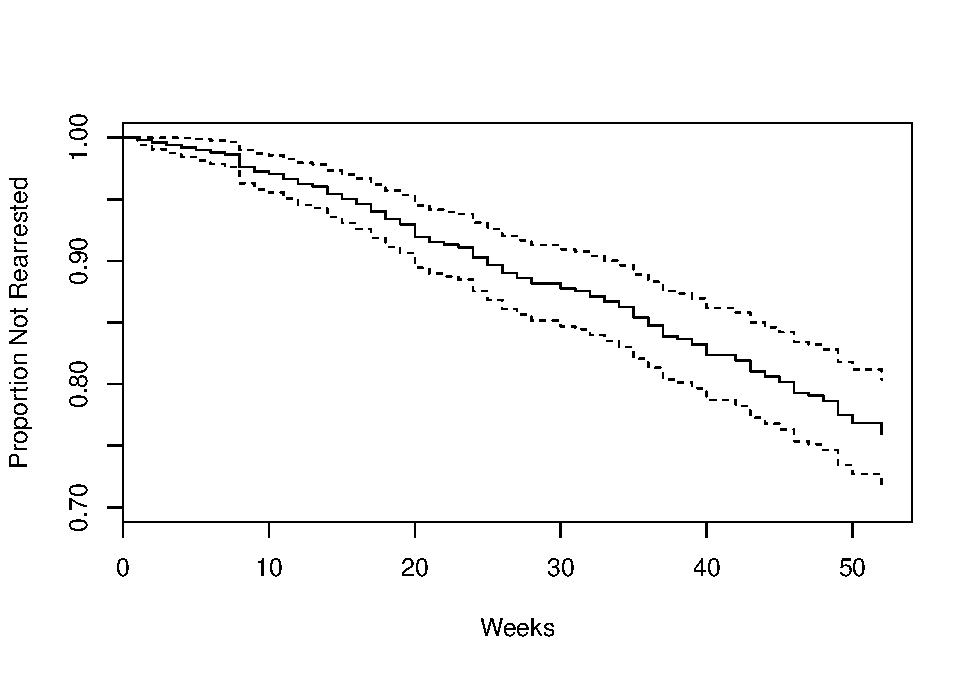
\includegraphics{datadown_files/figure-latex/unnamed-chunk-40-1.pdf}

\hypertarget{result}{%
\subsection{result}\label{result}}

\begin{itemize}
\tightlist
\item
  The covariates age and prio (prior convictions) have highly statistically significant coefficients, while the coefficient for fin (financial aid) is marginally significant
\item
  holding the other covariates constant, an additional year of age reduces the weekly hazard of rearrest by a factor of \(e^b = 0.944\) on average -- that is, by 5.6
\item
  likelihood-ratio, Wald, and score chi-square statistics: null hypothesis all of the β's are zero.
\end{itemize}

\hypertarget{further}{%
\section{further}\label{further}}

\begin{itemize}
\tightlist
\item
  assess the impact of financial aid on rearrest
\item
  new data frame with two rows, one for each value of fin; the other covariates are fixed to their average values
\end{itemize}

\begin{Shaded}
\begin{Highlighting}[]
\KeywordTok{attach}\NormalTok{(Rossi)}
\NormalTok{Rossi.fin <-}\StringTok{ }\KeywordTok{data.frame}\NormalTok{(}\DataTypeTok{fin=}\KeywordTok{c}\NormalTok{(}\DecValTok{0}\NormalTok{,}\DecValTok{1}\NormalTok{), }\DataTypeTok{age=}\KeywordTok{rep}\NormalTok{(}\KeywordTok{mean}\NormalTok{(age),}\DecValTok{2}\NormalTok{), }\DataTypeTok{race=}\KeywordTok{rep}\NormalTok{(}\KeywordTok{mean}\NormalTok{(race),}\DecValTok{2}\NormalTok{), }\DataTypeTok{wexp=}\KeywordTok{rep}\NormalTok{(}\KeywordTok{mean}\NormalTok{(wexp),}\DecValTok{2}\NormalTok{), }\DataTypeTok{mar=}\KeywordTok{rep}\NormalTok{(}\KeywordTok{mean}\NormalTok{(mar),}\DecValTok{2}\NormalTok{), }\DataTypeTok{paro=}\KeywordTok{rep}\NormalTok{(}\KeywordTok{mean}\NormalTok{(paro),}\DecValTok{2}\NormalTok{), }\DataTypeTok{prio=}\KeywordTok{rep}\NormalTok{(}\KeywordTok{mean}\NormalTok{(prio),}\DecValTok{2}\NormalTok{))}
\KeywordTok{detach}\NormalTok{()}
\KeywordTok{plot}\NormalTok{(}\KeywordTok{survfit}\NormalTok{(mod.allison, }\DataTypeTok{newdata=}\NormalTok{Rossi.fin), }\DataTypeTok{conf.int=}\NormalTok{T, }\DataTypeTok{lty=}\KeywordTok{c}\NormalTok{(}\DecValTok{1}\NormalTok{,}\DecValTok{2}\NormalTok{), }\DataTypeTok{ylim=}\KeywordTok{c}\NormalTok{(.}\DecValTok{6}\NormalTok{, }\DecValTok{1}\NormalTok{))}
\KeywordTok{legend}\NormalTok{(}\StringTok{"bottomleft"}\NormalTok{, }\DataTypeTok{legend=}\KeywordTok{c}\NormalTok{(}\StringTok{'fin = 0'}\NormalTok{, }\StringTok{'fin = 1'}\NormalTok{), }\DataTypeTok{lty=}\KeywordTok{c}\NormalTok{(}\DecValTok{1}\NormalTok{,}\DecValTok{2}\NormalTok{))}
\end{Highlighting}
\end{Shaded}

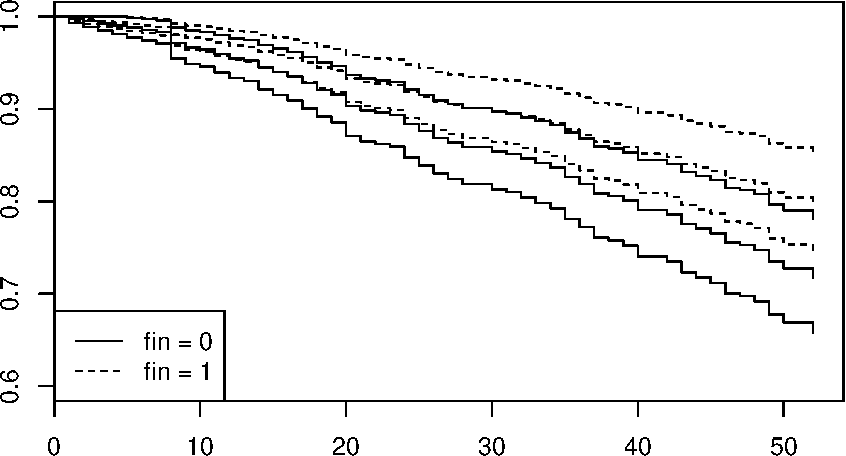
\includegraphics{datadown_files/figure-latex/unnamed-chunk-41-1.pdf}

\begin{itemize}
\tightlist
\item
  the higher estimated `survival' of those receiving financial aid, but the two confidence envelopes overlap substantially, even after 52 weeks
\end{itemize}

\hypertarget{time-dependent-covariates}{%
\section{Time-Dependent Covariates}\label{time-dependent-covariates}}

\begin{itemize}
\tightlist
\item
  treat the employed variable as a tim-dependent covariates with 52 weeks' record
\end{itemize}

\begin{Shaded}
\begin{Highlighting}[]
\KeywordTok{sum}\NormalTok{(}\OperatorTok{!}\KeywordTok{is.na}\NormalTok{(Rossi[,}\DecValTok{11}\OperatorTok{:}\DecValTok{62}\NormalTok{])) }\CommentTok{# record count}
\end{Highlighting}
\end{Shaded}

\begin{verbatim}
## [1] 19809
\end{verbatim}

\begin{Shaded}
\begin{Highlighting}[]
\NormalTok{Rossi2 <-}\StringTok{ }\KeywordTok{matrix}\NormalTok{(}\DecValTok{0}\NormalTok{, }\DecValTok{19809}\NormalTok{, }\DecValTok{14}\NormalTok{) }\CommentTok{# to hold new data set}
\KeywordTok{colnames}\NormalTok{(Rossi2) <-}\StringTok{ }\KeywordTok{c}\NormalTok{(}\StringTok{'start'}\NormalTok{, }\StringTok{'stop'}\NormalTok{, }\StringTok{'arresttime'}\NormalTok{, }\KeywordTok{names}\NormalTok{(Rossi)[}\DecValTok{1}\OperatorTok{:}\DecValTok{10}\NormalTok{], }\StringTok{'employed'}\NormalTok{)}

\NormalTok{row<-}\DecValTok{0}
\ControlFlowTok{for}\NormalTok{ (i }\ControlFlowTok{in} \DecValTok{1}\OperatorTok{:}\KeywordTok{nrow}\NormalTok{(Rossi)) \{ }
    \ControlFlowTok{for}\NormalTok{ (j }\ControlFlowTok{in} \DecValTok{11}\OperatorTok{:}\DecValTok{62}\NormalTok{) \{ }
        \ControlFlowTok{if}\NormalTok{ (}\KeywordTok{is.na}\NormalTok{(Rossi[i, j])) }\ControlFlowTok{next}
        \ControlFlowTok{else}\NormalTok{ \{}
\NormalTok{            row <-}\StringTok{ }\NormalTok{row }\OperatorTok{+}\StringTok{ }\DecValTok{1} \CommentTok{# increment row counter}
\NormalTok{            start <-}\StringTok{ }\NormalTok{j }\OperatorTok{-}\StringTok{ }\DecValTok{11} \CommentTok{# start time (previous week)}
\NormalTok{            stop <-}\StringTok{ }\NormalTok{start }\OperatorTok{+}\StringTok{ }\DecValTok{1} \CommentTok{# stop time (current week)}
\NormalTok{            arresttime <-}\StringTok{ }\ControlFlowTok{if}\NormalTok{ (stop }\OperatorTok{==}\StringTok{ }\NormalTok{Rossi[i, }\DecValTok{1}\NormalTok{] }\OperatorTok{&&}\StringTok{ }\NormalTok{Rossi[i, }\DecValTok{2}\NormalTok{] }\OperatorTok{==}\DecValTok{1}\NormalTok{) }\DecValTok{1} \ControlFlowTok{else} \DecValTok{0}
\NormalTok{            Rossi2[row,] <-}\StringTok{ }\KeywordTok{c}\NormalTok{(start, stop, arresttime, }\KeywordTok{unlist}\NormalTok{(Rossi[i, }\KeywordTok{c}\NormalTok{(}\DecValTok{1}\OperatorTok{:}\DecValTok{10}\NormalTok{, j)]))}
\NormalTok{            \}}
\NormalTok{        \}}
\NormalTok{\}}
\NormalTok{Rossi2 <-}\StringTok{ }\KeywordTok{as.data.frame}\NormalTok{(Rossi2)}
\KeywordTok{remove}\NormalTok{(i, j, row, start, stop, arresttime)}
\NormalTok{modallison2 <-}\StringTok{ }\KeywordTok{coxph}\NormalTok{(}\KeywordTok{Surv}\NormalTok{(start, stop, arresttime) }\OperatorTok{~}\StringTok{ }\NormalTok{fin }\OperatorTok{+}\StringTok{ }\NormalTok{age }\OperatorTok{+}\StringTok{ }\NormalTok{race }\OperatorTok{+}\StringTok{ }\NormalTok{wexp }\OperatorTok{+}\StringTok{ }\NormalTok{mar }\OperatorTok{+}\StringTok{ }\NormalTok{paro }\OperatorTok{+}\StringTok{ }\NormalTok{prio }\OperatorTok{+}\StringTok{ }\NormalTok{employed, }\DataTypeTok{data=}\NormalTok{Rossi2)}
\KeywordTok{summary}\NormalTok{(modallison2)}
\end{Highlighting}
\end{Shaded}

\begin{verbatim}
## Call:
## coxph(formula = Surv(start, stop, arresttime) ~ fin + age + race + 
##     wexp + mar + paro + prio + employed, data = Rossi2)
## 
##   n= 19809, number of events= 114 
## 
##             coef exp(coef) se(coef)     z Pr(>|z|)    
## fin      -0.3567    0.7000   0.1911 -1.87   0.0620 .  
## age      -0.0463    0.9547   0.0217 -2.13   0.0330 *  
## race      0.3387    1.4031   0.3096  1.09   0.2740    
## wexp     -0.0256    0.9748   0.2114 -0.12   0.9038    
## mar      -0.2937    0.7455   0.3830 -0.77   0.4431    
## paro     -0.0642    0.9378   0.1947 -0.33   0.7416    
## prio      0.0851    1.0889   0.0290  2.94   0.0033 ** 
## employed -1.3283    0.2649   0.2507 -5.30  1.2e-07 ***
## ---
## Signif. codes:  0 '***' 0.001 '**' 0.01 '*' 0.05 '.' 0.1 ' ' 1
## 
##          exp(coef) exp(-coef) lower .95 upper .95
## fin          0.700      1.429     0.481     1.018
## age          0.955      1.047     0.915     0.996
## race         1.403      0.713     0.765     2.574
## wexp         0.975      1.026     0.644     1.475
## mar          0.745      1.341     0.352     1.579
## paro         0.938      1.066     0.640     1.374
## prio         1.089      0.918     1.029     1.152
## employed     0.265      3.775     0.162     0.433
## 
## Concordance= 0.708  (se = 0.023 )
## Likelihood ratio test= 68.7  on 8 df,   p=9e-12
## Wald test            = 56.1  on 8 df,   p=3e-09
## Score (logrank) test = 64.5  on 8 df,   p=6e-11
\end{verbatim}

\hypertarget{model-diagnostics}{%
\section{Model Diagnostics}\label{model-diagnostics}}

\begin{itemize}
\tightlist
\item
  Checking Proportional Hazards
\end{itemize}

\begin{Shaded}
\begin{Highlighting}[]
\NormalTok{modallison3 <-}\StringTok{ }\KeywordTok{coxph}\NormalTok{(}\KeywordTok{Surv}\NormalTok{(week, arrest) }\OperatorTok{~}\StringTok{ }\NormalTok{fin }\OperatorTok{+}\StringTok{ }\NormalTok{age }\OperatorTok{+}\StringTok{ }\NormalTok{prio, }\DataTypeTok{data=}\NormalTok{Rossi)}
\NormalTok{modallison3}
\end{Highlighting}
\end{Shaded}

\begin{verbatim}
## Call:
## coxph(formula = Surv(week, arrest) ~ fin + age + prio, data = Rossi)
## 
##       coef exp(coef) se(coef)  z     p
## fin  -0.35      0.71     0.19 -2 0.068
## age  -0.07      0.94     0.02 -3 0.001
## prio  0.10      1.10     0.03  4 4e-04
## 
## Likelihood ratio test=29  on 3 df, p=2e-06
## n= 432, number of events= 114
\end{verbatim}

\begin{Shaded}
\begin{Highlighting}[]
\KeywordTok{cox.zph}\NormalTok{(modallison3)}
\end{Highlighting}
\end{Shaded}

\begin{verbatim}
##         chisq df     p
## fin    0.0638  1 0.801
## age    6.3255  1 0.012
## prio   0.5187  1 0.471
## GLOBAL 7.1367  3 0.068
\end{verbatim}

\begin{Shaded}
\begin{Highlighting}[]
\KeywordTok{par}\NormalTok{(}\DataTypeTok{mfrow=}\KeywordTok{c}\NormalTok{(}\DecValTok{2}\NormalTok{,}\DecValTok{2}\NormalTok{))}
\KeywordTok{plot}\NormalTok{(}\KeywordTok{cox.zph}\NormalTok{(modallison3))}
\end{Highlighting}
\end{Shaded}

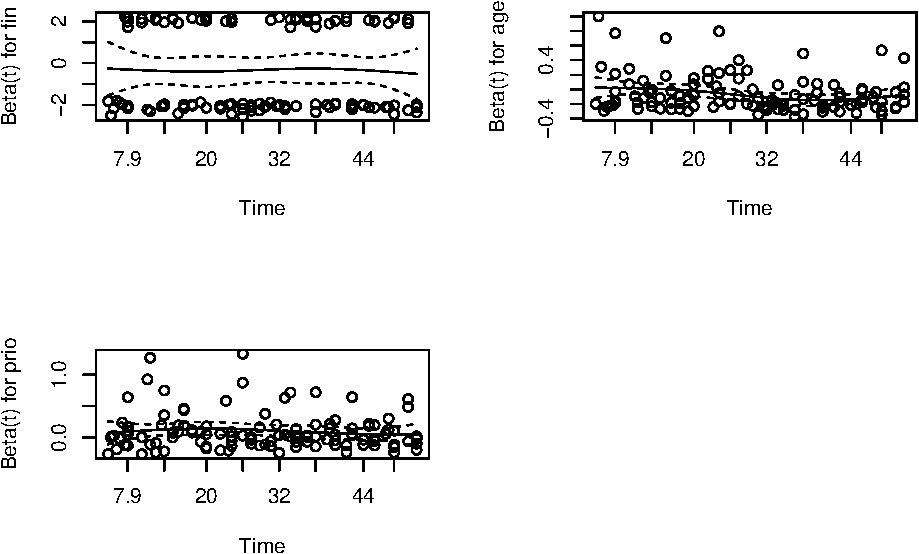
\includegraphics{datadown_files/figure-latex/unnamed-chunk-43-1.pdf}

\begin{itemize}
\tightlist
\item
  there appears to be a trend in the plot for age, with the age effect declining with time
\end{itemize}

\begin{Shaded}
\begin{Highlighting}[]
\NormalTok{modallison4 <-}\StringTok{ }\KeywordTok{coxph}\NormalTok{(}\KeywordTok{Surv}\NormalTok{(start,stop,arresttime)}\OperatorTok{~}\NormalTok{fin}\OperatorTok{+}\NormalTok{age}\OperatorTok{+}\NormalTok{age}\OperatorTok{:}\NormalTok{stop}\OperatorTok{:}\NormalTok{stop}\OperatorTok{+}\NormalTok{prio, }\DataTypeTok{data =}\NormalTok{ Rossi2)}
\NormalTok{modallison4}
\end{Highlighting}
\end{Shaded}

\begin{verbatim}
## Call:
## coxph(formula = Surv(start, stop, arresttime) ~ fin + age + age:stop:stop + 
##     prio, data = Rossi2)
## 
##            coef exp(coef) se(coef)    z     p
## fin      -0.349     0.706    0.190 -1.8 0.067
## age       0.032     1.033    0.039  0.8 0.413
## prio      0.098     1.103    0.027  3.6 3e-04
## age:stop -0.004     0.996    0.001 -2.6 0.009
## 
## Likelihood ratio test=36  on 4 df, p=3e-07
## n= 19809, number of events= 114
\end{verbatim}

\begin{itemize}
\item
  the coefficient for the interaction is negative and highly statistically significant: The effect of age declines with time
\item
  use residual to find influential observations
\end{itemize}

\hypertarget{reference}{%
\section{Reference}\label{reference}}

\begin{itemize}
\tightlist
\item
  \href{http://cran.r-project.org/doc/contrib/Fox-Companion/appendix-cox-regression.pdf}{Cox Proportional-Hazards Regression for Survival Data}
\item
  \href{http://ehp.niehs.nih.gov/1104049/}{Real Cases}
\end{itemize}

\hypertarget{epid}{%
\chapter{流行病学}\label{epid}}

\hypertarget{ux58f0ux660e}{%
\section{声明}\label{ux58f0ux660e}}

\begin{itemize}
\tightlist
\item
  本笔记来自于波士顿大学\href{http://sphweb.bumc.bu.edu/otlt/MPH-Modules/Modules_Menu.html}{在线教程}与北卡大学教堂山分校的\href{https://www.coursera.org/learn/epidemiology/outline}{公开课}
\item
  二手知识,谨防消化不良
\item
  翻译有误之处见谅,烦请\href{mailto:yufreecas@gmail.com}{告知},谢谢!
\end{itemize}

\hypertarget{ux65e9ux671fux75beux75c5ux7684ux6982ux5ff5}{%
\section{早期疾病的概念}\label{ux65e9ux671fux75beux75c5ux7684ux6982ux5ff5}}

\begin{itemize}
\tightlist
\item
  渔猎时期主要问题是食物的供应与营养均衡问题
\item
  农耕时期开始群居,出现疾病的流行问题

  \begin{itemize}
  \tightlist
  \item
    神秘主义,迷信与神的惩罚
  \item
    希波克拉底:理性思考疾病起源,提出体液学说
  \item
    欧洲流行300多年的黑死病,开始认为病因是``瘴气'',其实是老鼠跳蚤上细菌
  \item
    没有验证病因与疾病关系的方法与预防措施
  \end{itemize}
\item
  工业革命时期城市规模迅速扩大,分工细化,出现职业暴露健康问题
\end{itemize}

\hypertarget{ux8fd1ux4ee3ux6d41ux884cux75c5ux5b66ux5173ux952eux4ebaux7269}{%
\section{近代流行病学关键人物}\label{ux8fd1ux4ee3ux6d41ux884cux75c5ux5b66ux5173ux952eux4ebaux7269}}

\begin{itemize}
\tightlist
\item
  Girolamo Fracastoro (1546) 认为疾病来自种子
\item
  John Graunt - The Bills of Mortality (1662) 记录伦敦死亡率,出生率数据并进行分析
\item
  Anton van Leeuwenhouk (1670s) 显微镜之父,首先观察到细胞
\item
  John Pringle and ``Jail Fever'' (1740s) 研究军队与监狱卫生与疾病并讨论了与伤寒的关系
\item
  James Lind and Scurvy (1754) 进行了第一例临床控制实验,验证柑橘对坏血病的治疗作用
\item
  Francois Broussais \& Pierre Louis (1832) 提出放血疗法,没有验证但沿用几个世纪
\item
  Ignaz Semmelweis and Oliver Wendell Holmes (1840s) 前者发现了某种产科疾病是由刚解剖完尸体的学生引入的,后者推行了疾病可能来源于医护人员的理念而饱受争议
\item
  John Snow - The Father of Epidemiology (1850s) 流行病学之父,研究并验证了霍乱与城市供水的关系
\item
  Louis Pasteur (late 1800) 提出巴氏消毒法与疫苗理论
\item
  公共卫生的概念 (1850-1875) 起源于人口统计及18世纪的启蒙运动例如功利主义的兴起对公众健康的关注
\end{itemize}

\hypertarget{ux73b0ux4ee3ux6162ux6027ux75c5ux6d41ux884cux75c5ux5b66}{%
\section{现代慢性病流行病学}\label{ux73b0ux4ee3ux6162ux6027ux75c5ux6d41ux884cux75c5ux5b66}}

\begin{itemize}
\tightlist
\item
  肺癌:工业革命后的肺癌发病率很高,普遍认为是工厂公路导致,但后续研究表明吸烟可能是主要因素,该研究促进了病例对照研究的发展
\item
  \href{http://www.framinghamheartstudy.org/}{佛雷明翰心脏病研究}:48年起追踪心脏病研究,已持续三代人
\end{itemize}

\begin{Shaded}
\begin{Highlighting}[]
\NormalTok{knitr}\OperatorTok{::}\KeywordTok{include_graphics}\NormalTok{(}\StringTok{'images/Framingham1.jpg'}\NormalTok{)}
\end{Highlighting}
\end{Shaded}

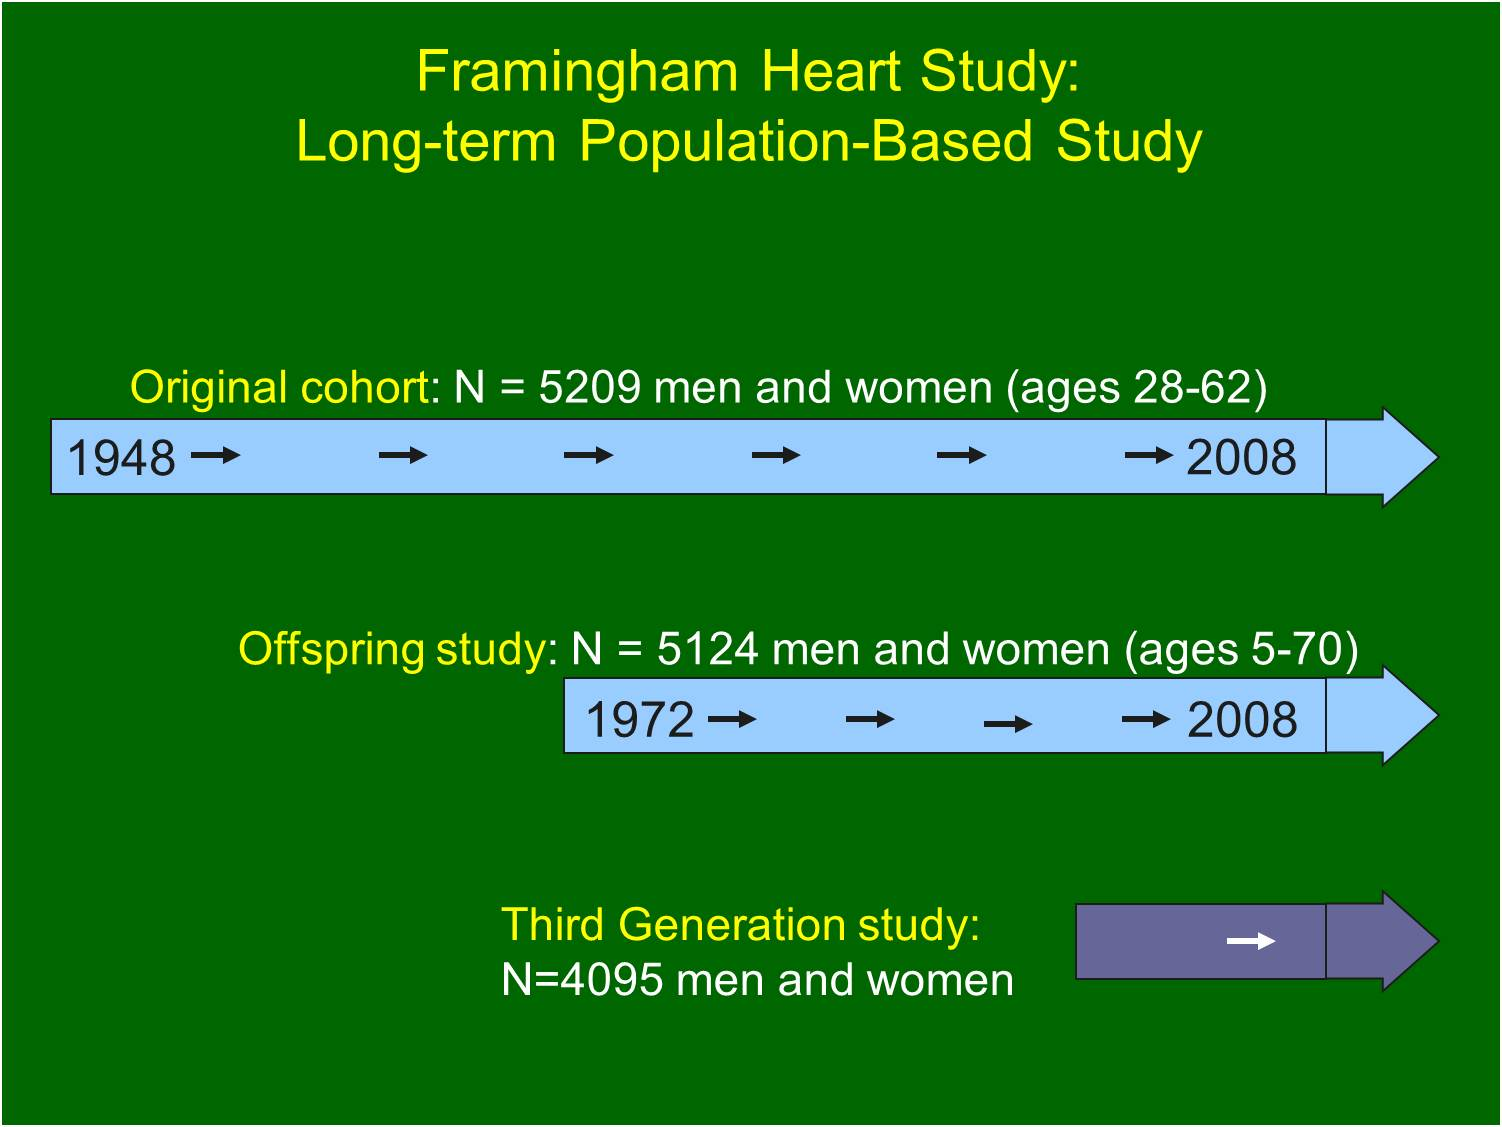
\includegraphics[width=20.86in]{images/Framingham1}

\hypertarget{ux6d41ux884cux75c5ux5b66ux57faux672cux6982ux5ff5}{%
\section{流行病学基本概念}\label{ux6d41ux884cux75c5ux5b66ux57faux672cux6982ux5ff5}}

\hypertarget{ux57faux672cux5047ux8bbe}{%
\subsection{基本假设}\label{ux57faux672cux5047ux8bbe}}

\begin{itemize}
\tightlist
\item
  病有病因非随机
\item
  病因可察可研究
\end{itemize}

\hypertarget{ux5b9aux4e49}{%
\subsection{定义}\label{ux5b9aux4e49}}

\begin{itemize}
\item
  研究人群中疾病分布与成因的学科

  \begin{longtable}[]{@{}cc@{}}
  \toprule
  阶段 & 研究类型\tabularnewline
  \midrule
  \endhead
  观察\&形成假说 & 案例研究/断面研究/生态学研究\tabularnewline
  观察研究假设检验 & 病例控制研究与队列研究\tabularnewline
  临床研究假设检验 & 临床实验\tabularnewline
  \bottomrule
  \end{longtable}
\end{itemize}

\hypertarget{ux63cfux8ff0ux6027ux6d41ux884cux75c5ux5b66}{%
\section{描述性流行病学}\label{ux63cfux8ff0ux6027ux6d41ux884cux75c5ux5b66}}

\begin{itemize}
\tightlist
\item
  关注不同时间、地点、人群的差异、相似性与相关性,形成假说
\item
  案例:传染病暴发

  \begin{itemize}
  \tightlist
  \item
    早期关注案例采访,寻找共同点
  \item
    对地理位置作图寻找空间关系
  \item
    对时间趋势作图寻找变化规律
  \end{itemize}
\item
  流行曲线:横轴日期,纵轴新增病例

  \begin{itemize}
  \tightlist
  \item
    点源爆发:单峰,潜伏期相对一致
  \end{itemize}
\end{itemize}

\begin{Shaded}
\begin{Highlighting}[]
\NormalTok{knitr}\OperatorTok{::}\KeywordTok{include_graphics}\NormalTok{(}\StringTok{'images/epidemic%20curve.jpg'}\NormalTok{)}
\end{Highlighting}
\end{Shaded}

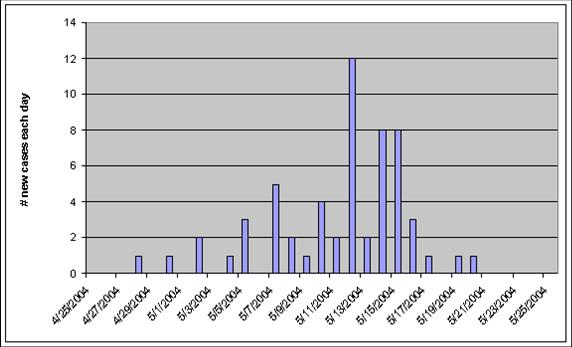
\includegraphics{images/epidemic curve.jpg}
- 持续源爆发:单峰,潜伏期持续出现

\begin{Shaded}
\begin{Highlighting}[]
\NormalTok{knitr}\OperatorTok{::}\KeywordTok{include_graphics}\NormalTok{(}\StringTok{'images/EpidemicCurve_Cholera.png'}\NormalTok{)}
\end{Highlighting}
\end{Shaded}

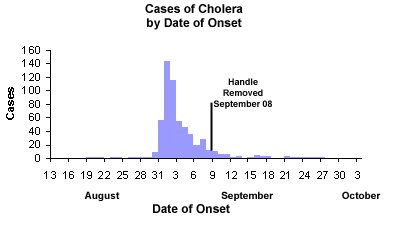
\includegraphics[width=5.5in]{images/EpidemicCurve_Cholera}
- 逐步流行:多峰,存在人对人传染

\begin{Shaded}
\begin{Highlighting}[]
\NormalTok{knitr}\OperatorTok{::}\KeywordTok{include_graphics}\NormalTok{(}\StringTok{'images/EpidemicCurve_Measles.png'}\NormalTok{)}
\end{Highlighting}
\end{Shaded}

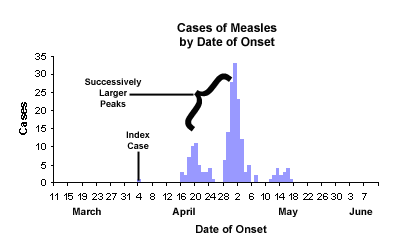
\includegraphics[width=5.53in]{images/EpidemicCurve_Measles}

\hypertarget{ux75beux75c5ux7206ux53d1ux7684ux7814ux7a76ux6b65ux9aa4}{%
\subsection{疾病爆发的研究步骤}\label{ux75beux75c5ux7206ux53d1ux7684ux7814ux7a76ux6b65ux9aa4}}

\begin{itemize}
\tightlist
\item
  准备研究
\item
  验证诊断与爆发的存在
\item
  定义案例并寻找案例
\item
  进行描述性流行病学研究确定时间、地点与人群的差异
\item
  生成爆发原因与来源的假设
\item
  假设检验
\item
  制定控制与预防措施
\item
  交流研究发现
\end{itemize}

\hypertarget{ux6162ux6027ux75c5ux7684ux63cfux8ff0ux6027ux6d41ux884cux75c5ux5b66}{%
\subsection{慢性病的描述性流行病学}\label{ux6162ux6027ux75c5ux7684ux63cfux8ff0ux6027ux6d41ux884cux75c5ux5b66}}

\begin{itemize}
\tightlist
\item
  人群特质:年龄,性别,种族,职业,饮食习惯,宗教习惯,业余活动等
\item
  地点:慢性病地域差距
\item
  时间:大趋势,季节性,片断性
\item
  其他:环境变化,诊断精度,医疗水平,人群年龄分布
\end{itemize}

\hypertarget{ux63cfux8ff0ux6d41ux884cux75c5ux5b66ux5206ux7c7b}{%
\subsection{描述流行病学分类}\label{ux63cfux8ff0ux6d41ux884cux75c5ux5b66ux5206ux7c7b}}

\begin{itemize}
\tightlist
\item
  病例报道 单个案例

  \begin{itemize}
  \tightlist
  \item
    \href{http://www.thelancet.com/journals/lancet/article/PIIS0140-6736(83)92082-2/abstract\#}{艾滋病血液传播的发现}
  \item
    \href{http://www.nejm.org/doi/full/10.1056/NEJMoa050382\#t=abstract}{无注射狂犬疫苗后痊愈}
  \end{itemize}
\item
  系列病例 多个案例

  \begin{itemize}
  \tightlist
  \item
    \href{http://www.nejm.org/doi/pdf/10.1056/NEJM198112103052401}{男同性恋间获得性免疫缺陷传染}
  \end{itemize}
\item
  断面研究 同一时间对特定人群的健康状况与风险因子进行调查

  \begin{itemize}
  \tightlist
  \item
    \href{http://www.cdc.gov/nchs/nhis.htm}{HIS}
  \item
    \href{http://www.cdc.gov/nchs/nhanes.htm}{NHANES}
  \end{itemize}
\item
  生态学研究 以群体为单位研究区域平均暴露状况
\end{itemize}

\hypertarget{ux5206ux6790ux6d41ux884cux75c5ux5b66}{%
\section{分析流行病学}\label{ux5206ux6790ux6d41ux884cux75c5ux5b66}}

\begin{itemize}
\tightlist
\item
  不同于描述流行病学提出假设,分析流行病学进行假设检验
\item
  队列研究:定义基线与风险人群

  \begin{itemize}
  \tightlist
  \item
    前瞻性队列研究:参与者参加的时候不出现健康效应
  \item
    回顾性队列研究:根据已经出现的健康效应反向追查风险因子
  \end{itemize}
\item
  临床实验:风险因子由研究人员指定
\item
  病例对照研究:不用来研究发病率,侧重风险比,不追踪,根据已有状况回溯,对幸存者采样,适合稀有病症的研究
\end{itemize}

\begin{Shaded}
\begin{Highlighting}[]
\NormalTok{knitr}\OperatorTok{::}\KeywordTok{include_graphics}\NormalTok{(}\StringTok{'images/paste_image47.jpg'}\NormalTok{)}
\end{Highlighting}
\end{Shaded}

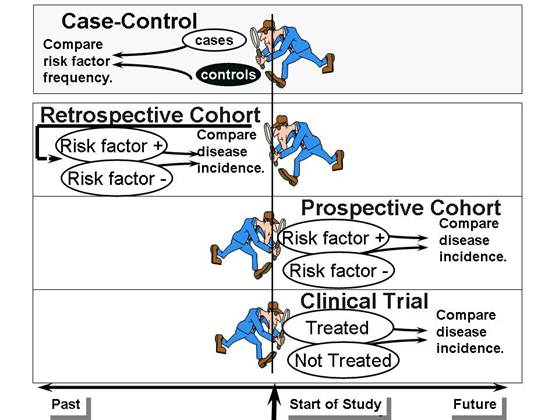
\includegraphics[width=7.76in]{images/paste_image47}

\begin{itemize}
\tightlist
\item
  判断流程

  \begin{itemize}
  \tightlist
  \item
    是否个人(生态学研究)
  \item
    是否有对照(系列案例)
  \item
    是否追踪(断面研究)
  \item
    是否不先选取出现健康状况的组(病例对照研究)
  \item
    是否不出现健康状况(回顾队列研究)
  \item
    是否指定对照组(前瞻队列研究)
  \item
    临床实验
  \end{itemize}
\end{itemize}

\hypertarget{ux75beux75c5ux76d1ux63a7}{%
\section{疾病监控}\label{ux75beux75c5ux76d1ux63a7}}

\begin{itemize}
\tightlist
\item
  早期教堂记录出生率与死亡率
\item
  1662 John Graunt ``Bills of Mortality''
\item
  1837 英国建立 General Registrar's Office 记录市民出生、死亡与婚姻
\item
  John Snow 对霍乱数据的分析
\item
  1842 马萨诸塞州开始记录出生死亡状况
\item
  1901 全美开始记录疾病流行状况
\item
  1925 强制执行疾病监控
\item
  目前基本是CDC控制,除了强制汇报,也有主动收集
\item
  综合疾控,不等确诊收集症状,例如google flu
\end{itemize}

\hypertarget{ux75beux75c5ux9891ux7387ux7684ux6d4bux91cf}{%
\section{疾病频率的测量}\label{ux75beux75c5ux9891ux7387ux7684ux6d4bux91cf}}

\hypertarget{ux4ebaux7fa4}{%
\subsection{人群}\label{ux4ebaux7fa4}}

\begin{itemize}
\tightlist
\item
  固定人群(相对固定,或由事件定义)
\item
  动态人群(由当前状态决定的人群)
\end{itemize}

\hypertarget{ux60a3ux75c5ux7387prevalence}{%
\subsection{患病率(prevalence)}\label{ux60a3ux75c5ux7387prevalence}}

表示在指定时间里具有某种健康效应的人群比例,非新增

\[prevalence = \frac{affected individuals}{total individuals in the population}\]

举例:患病率0.25表示人群中有25\%的人在指定的时间段里受某种健康效应影响

经常会导致因果推断不准,因为影响因素产生的效应被本来的效应覆盖了

\begin{Shaded}
\begin{Highlighting}[]
\NormalTok{knitr}\OperatorTok{::}\KeywordTok{include_graphics}\NormalTok{(}\StringTok{"images/paste_image18.jpg"}\NormalTok{)}
\end{Highlighting}
\end{Shaded}

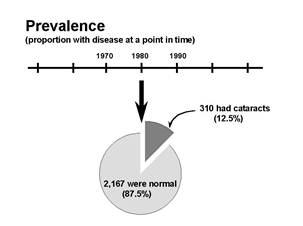
\includegraphics[width=4.21in]{images/paste_image18}

\hypertarget{ux98ceux9669risk}{%
\subsection{风险(risk)}\label{ux98ceux9669risk}}

也称作发病率(incidence或cumulative incidence),表示在一段\textbf{给定时间}里\textbf{新增}某种健康效应的比例

\[risk = \frac{new cases}{total individuals at risk}\]

举例:5年风险0.1表示在5年里某个个体有10\%的几率出现某种健康效应

前瞻性研究(prospective studies)常用,但控制性研究(case-control studies)里总体风险无法确定,不能使用。

\hypertarget{ux6bd4ux7387rate}{%
\subsection{比率(rate)}\label{ux6bd4ux7387rate}}

也称作发病率比率(incidence rates)表示在一个人群中某种健康效应出现的速度。单位为每个人年,个人年表示风险个体参与研究到出现健康效应的总时间

\[rate = \frac{new cases}{total person-time at risk}\]

举例:0.1案例每个人年表示对于每10个人追踪1年或2个人追踪5年将会有一个案例出现

人群无限状态下,有

\[risk = rate \cdot time\]

考虑到人口的指数衰减,有

\[risk = 1 - exp(- rate \cdot times)\]

当风险率非恒定时,或者对时间分段计算,或者进行生存分析

人群出现稳态时,有

\[\frac{prevalence}{1-prevalence} = rate \cdot Avg.Duration\]

当患病率很低时,有

\[prevalence = rate \cdot Avg.Duration\]

疾病的持续期可计算为

\[Avg.Duration = \frac{prevalence}{rate}\]

\hypertarget{ux5176ux4ed6ux9891ux7387ux6d4bux91cf}{%
\subsection{其他频率测量}\label{ux5176ux4ed6ux9891ux7387ux6d4bux91cf}}

\begin{itemize}
\tightlist
\item
  分类比率:如年龄,性别,种族等
\item
  病态比率:不致命的状态
\item
  死亡率
\item
  致死率:患病中导致死亡的比率
\item
  攻击率:短期食物中毒
\item
  生育率:育龄妇女一年内生育新生儿的比率
\item
  新生儿死亡率:一岁以下新生儿死亡率
\item
  特殊患病率:体检率,新生儿感染率,非新增
\end{itemize}

\hypertarget{ux8054ux7cfbux6d4bux91cf}{%
\section{联系测量}\label{ux8054ux7cfbux6d4bux91cf}}

\begin{itemize}
\tightlist
\item
  测定频率不涉及对比,探索关系需要对比
\item
  不同暴露状态下的频率差或者比表征
\end{itemize}

\hypertarget{ux98ceux9669ux6bd4ux4e0eux6bd4ux7387ux6bd4risk-ratio-rate-ratio}{%
\subsection{风险比与比率比(risk ratio rate ratio)}\label{ux98ceux9669ux6bd4ux4e0eux6bd4ux7387ux6bd4risk-ratio-rate-ratio}}

\[risk ratio = \frac{risk_{exposed}}{risk_{unexposed}}\]

\[rate ratio = \frac{rate_{exposed}}{rate_{unexposed}}\]

表示暴露与健康效应的关系强度,1表示无关,但比例关系不能给出绝对差异
表述风险比不要使用更多或更少,如果更多或更少需要减一除以风险比:相比不服用,服用阿司匹林有0.57倍的心肌梗死风险或43\%的风险下降

\hypertarget{ux5bf9ux7167ux7ec4}{%
\subsection{对照组}\label{ux5bf9ux7167ux7ec4}}

暴露量最小的一组通常作为风险比计算中的对照组

\hypertarget{ux98ceux9669ux5deerisk-difference}{%
\subsection{风险差(risk difference)}\label{ux98ceux9669ux5deerisk-difference}}

\[risk = risk_{exposed} - risk_{unexposed} = \frac{cases in exposed group}{total at risk in exposed group} - \frac{cases in control group}{total at risk in control group}\]

正数表明对某种健康效应有促进作用,负数表示有抑制作用,要指明时间区段

\hypertarget{ux5f52ux56e0ux6bd4ux4f8battributable-proportion-among-the-exposed}{%
\subsection{归因比例(Attributable Proportion Among the Exposed)}\label{ux5f52ux56e0ux6bd4ux4f8battributable-proportion-among-the-exposed}}

\[attributable proportion = \frac{risk ratio - 1}{risk ratio}\]

暴露组风险中归因于该原因的比例

\hypertarget{ux4ebaux7fa4ux5f52ux56e0ux6bd4ux4f8bpopulation-attributable-fraction}{%
\subsection{人群归因比例(Population Attributable Fraction)}\label{ux4ebaux7fa4ux5f52ux56e0ux6bd4ux4f8bpopulation-attributable-fraction}}

\[population Attributable Fraction = (proportion of cases exposed) \cdot (attributable proportion in the exposed)\]

人群中风险归于该原因的比例

\hypertarget{ux80dcux7387ux6bd4odds-ratio}{%
\subsection{胜率比(odds ratio)}\label{ux80dcux7387ux6bd4odds-ratio}}

\[odds ratios = \frac{odds_{exposed}}{odds_{unexposed}}\]

常用在控制性研究里替代风险比或比率比,这时风险比无法计算,但几率比可以在总体效应比较小与特殊采样技术使用的时候近似于风险比或比率比,解释起来与它们一致

\hypertarget{ux968fux673aux8befux5dee}{%
\section{随机误差}\label{ux968fux673aux8befux5dee}}

\begin{itemize}
\tightlist
\item
  偏差,混杂与随机误差是流行病学采样中最常见问题
\item
  随机误差也是采样误差
\item
  置信区间用来表示随机误差而非混杂偏差等误差
\item
  95\%置信区间与p值计算方法一致,可用来判断是否统计显著
\end{itemize}

\hypertarget{ux7814ux7a76ux9053ux5fb7}{%
\section{研究道德}\label{ux7814ux7a76ux9053ux5fb7}}

\begin{itemize}
\tightlist
\item
  无论目的如何,以人作为研究对象是不道德的
\item
  纳粹在二战期间集中营里使用人作为研究对象,1946年审批时提出Nuremberg Code:
\end{itemize}

\begin{quote}
Voluntary consent of the human subject is absolutely essential.
The experiment must yield generalizable knowledge that could not be obtained in any other way and is not random and unnecessary in nature.
Animal experimentation should precede human experimentation.
All unnecessary physical and mental suffering and injury should be avoided.
No experiment should be conducted if there is reason to believe that death or disabling injury will occur.
The degree of risk to subjects should never exceed the humanitarian importance of the problem.
Risks to the subjects should be minimized through proper preparations.
Experiments should only be conducted by scientifically qualified investigators.
Subjects should always be at liberty to withdraw from experiments.
Investigators must be ready to end the experiment at any stage if there is cause to believe that continuing the experiment is likely to result in injury, disability or death to the subject.
\end{quote}

\begin{itemize}
\tightlist
\item
  1964年,\href{http://www.wma.net/en/60about/70history/01declarationHelsinki/index.html}{WMA}接受赫尔辛基宣言
\item
  塔斯基吉梅毒研究,没有征得患者同意,也没有进行有效治疗,1972年泄漏,1974年美国出台\href{http://www.hhs.gov/ohrp/humansubjects/guidance/45cfr46.html}{人类被试保护法案},所有涉及人的研究需要通过\href{http://www.hhs.gov/ohrp/humansubjects/guidance/45cfr46.html\#46.107}{IRB}审核
\item
  1978年,议会出台\href{http://www.hhs.gov/ohrp/policy/belmont.html}{人类被试研究指南}
\item
  法律不强制,但基金一般有相关要求
\item
  相信研究有益等同于对其怀疑才可进行
\item
  安慰剂可以使用,但要保证患者最终能得到最好的治疗
\end{itemize}

\hypertarget{ux4e34ux5e8aux5b9eux9a8c}{%
\section{临床实验}\label{ux4e34ux5e8aux5b9eux9a8c}}

\begin{itemize}
\tightlist
\item
  分为预防性与治疗性干涉研究
\item
  新药研发的\href{https://clinicaltrials.gov/ct2/info/glossary\#phasel}{四阶段}

  \begin{itemize}
  \tightlist
  \item
    8-80人小规模评价安全性,副作用及副作用出现的剂量
  \item
    80-200人中等规模测试有效性,副作用及与剂量的关系
  \item
    200-40,000人大规模测试其与当前治疗方式的副作用强度
  \item
    推向市场后的监测,测试罕见但严重的副作用,例如\href{http://sphweb.bumc.bu.edu/otlt/MPH-Modules/EP/EP713_ClinicalTrials/H1N1_Surveillance.pdf}{H1N1疫苗}
  \end{itemize}
\end{itemize}

\hypertarget{ux7814ux7a76ux5bf9ux8c61}{%
\subsection{研究对象}\label{ux7814ux7a76ux5bf9ux8c61}}

\begin{itemize}
\tightlist
\item
  人群分层考虑是否为目标人群及是否愿意参加
\item
  内部验证准确性,外部验证广泛性
\item
  样本数由功效决定,由于疾病发病率低,很小的差异也需要很大的样本来保证功效
\end{itemize}

\hypertarget{ux5bf9ux7167ux7ec4ux4e0eux63a7ux5236ux7ec4}{%
\subsection{对照组与控制组}\label{ux5bf9ux7167ux7ec4ux4e0eux63a7ux5236ux7ec4}}

\begin{itemize}
\tightlist
\item
  排除混杂因素需要考虑除考察因素外其他因素在研究客体中分配均匀
\item
  分配方法包括自我前后对比与随机非随机分配
\item
  屏蔽

  \begin{itemize}
  \tightlist
  \item
    单盲:被试不知道是否是处理组
  \item
    双盲:研究人员与被试都不知道处理组
  \item
    三盲:进行处理的人也不知道是否是处理组
  \end{itemize}
\item
  安慰剂(placebo),也就是无效药
\item
  装假(sham),假装进行某个操作流程(有道德风险)
\item
  安慰剂效应:接受治疗的人都认为会从中收益,即使知道是安慰剂也会产生该\href{http://journals.plos.org/plosone/article?id=10.1371/journal.pone.0015591}{效应}
\item
  服从度,处理组与控制组要区分明显,内部一致

  \begin{itemize}
  \tightlist
  \item
    设计尽量简单
  \item
    被试生活规律
  \item
    通知明确
  \item
    实时追踪
  \item
    屏蔽处理信息
  \item
    对不服从的仔细询问,收集未使用药片,收集血液尿样进行评价
  \end{itemize}
\item
  掉队会导致功效降低及存在偏误
\end{itemize}

\hypertarget{ux4e34ux5e8aux5206ux6790ux4e2dux7684ux95eeux9898}{%
\subsection{临床分析中的问题}\label{ux4e34ux5e8aux5206ux6790ux4e2dux7684ux95eeux9898}}

\begin{itemize}
\tightlist
\item
  随即控制时要给出基线信息
\item
  混杂因素可能不在基线里而是直接影响结果
\item
  如果混杂因素在调整前后影响结果超过10\%,那么就要进行调整- 希望被处理分析,保证处理与对照中接受治疗的意愿接近
\item
  二次分析,只对接受的人进行结果分析,失去随机性与一定样本数及混杂控制
\item
  某项研究同时有利弊,利大于弊,是否继续研究?
\item
  预防花费如果很高,是否值得推荐?
\end{itemize}

\hypertarget{ux961fux5217ux7814ux7a76}{%
\section{队列研究}\label{ux961fux5217ux7814ux7a76}}

\hypertarget{ux524dux77bbux6027ux961fux5217ux7814ux7a76}{%
\subsection{前瞻性队列研究}\label{ux524dux77bbux6027ux961fux5217ux7814ux7a76}}

\begin{itemize}
\tightlist
\item
  研究开始时没病,记录基线,追踪个人
\item
  案例:\href{http://www.ncbi.nlm.nih.gov/pubmed/7654270}{BMI与心脏病关系}
\end{itemize}

\hypertarget{ux56deux987eux6027ux961fux5217ux7814ux7a76}{%
\subsection{回顾性队列研究}\label{ux56deux987eux6027ux961fux5217ux7814ux7a76}}

\begin{itemize}
\tightlist
\item
  适合职业暴露,回溯暴露状况
\item
  案例:\href{http://www.cdc.gov/parasites/giardia/}{游泳池污染事件}
\end{itemize}

\hypertarget{ux53ccux5411ux961fux5217ux7814ux7a76}{%
\subsection{双向队列研究}\label{ux53ccux5411ux961fux5217ux7814ux7a76}}

\begin{itemize}
\tightlist
\item
  同时进行前瞻性与回顾性队列研究 较少见
\item
  案例:橙剂喷洒飞行员追踪,急性与慢性暴露
\end{itemize}

\hypertarget{ux56faux5b9aux961fux5217ux4e0eux5f00ux653eux961fux5217}{%
\subsection{固定队列与开放队列}\label{ux56faux5b9aux961fux5217ux4e0eux5f00ux653eux961fux5217}}

\begin{itemize}
\tightlist
\item
  固定队列表示人数固定或只能减少,例如日本原子弹受害者追踪,多数研究是固定队列
\item
  开放队列表示人数动态,可随时加入
\end{itemize}

\hypertarget{ux7814ux7a76ux5bf9ux8c61-1}{%
\subsection{研究对象}\label{ux7814ux7a76ux5bf9ux8c61-1}}

\begin{itemize}
\tightlist
\item
  一般人群队列或特殊暴露队列(事件幸存者)
\item
  对比组越接近越好,信息收集越全越好

  \begin{itemize}
  \tightlist
  \item
    内部比对:同队列未暴露被试,肥胖调查中不肥胖的人
  \item
    外部比对:内部不存在未暴露时,例如化学品职业暴露
  \item
    一般人群比对:从国家抽取基础数据,但因为健康工人效应现在不常用,可使用标准死亡率(SMR)或标准流行指数(SIR)来测量联系,也就是用基础数据计算期望值与实际值的对比
  \end{itemize}
\item
  健康工人效应:能工作的工人比一般人群要健康
\end{itemize}

\hypertarget{ux961fux5217ux8ffdux8e2a}{%
\subsection{队列追踪}\label{ux961fux5217ux8ffdux8e2a}}

\begin{itemize}
\tightlist
\item
  队列研究一般开始时没有偏见
\item
  追踪率低于60\%不可靠,丢失20\%可能因掉队原因关联结果导致偏误
\item
  不愿参与会导致偏差
\item
  回溯研究会因保留疾病比例高于保留正常病例的原因导致选择偏误
\end{itemize}

\hypertarget{ux4f18ux70b9}{%
\subsection{优点}\label{ux4f18ux70b9}}

\begin{itemize}
\tightlist
\item
  直接给出暴露与效应的时间序列关系
\item
  可直接计算疾病的风险率
\item
  可用来评价稀有暴露
\item
  可用来同时评价多种暴露
\item
  基本无选择偏误
\end{itemize}

\hypertarget{ux524dux77bbux6027ux961fux5217ux7814ux7a76ux7f3aux70b9}{%
\subsection{前瞻性队列研究缺点}\label{ux524dux77bbux6027ux961fux5217ux7814ux7a76ux7f3aux70b9}}

\begin{itemize}
\tightlist
\item
  耗时长
\item
  费用高
\item
  不适用稀有疾病
\item
  不适用潜伏期长疾病
\item
  掉队会导致偏差
\end{itemize}

\hypertarget{ux56deux987eux6027ux961fux5217ux7814ux7a76ux7f3aux70b9}{%
\subsection{回顾性队列研究缺点}\label{ux56deux987eux6027ux961fux5217ux7814ux7a76ux7f3aux70b9}}

\begin{itemize}
\tightlist
\item
  不适用稀有疾病
\item
  记录不匹配研究需要结果不好
\item
  过去记录丢失混杂因素信息
\item
  暴露组与对比组很难区分
\item
  掉队会导致偏差
\end{itemize}

\hypertarget{ux504fux8bef}{%
\subsection{偏误}\label{ux504fux8bef}}

\begin{itemize}
\tightlist
\item
  选择人群无法代表群体
\item
  产生原因

  \begin{itemize}
  \tightlist
  \item
    在病例控制研究中控制组没有代表性
  \item
    追踪丢失率在控制与处理组不同
  \item
    是否愿意参加影响暴露与结果
  \item
    健康工人效应(职业暴露)
  \item
    诊断标准不同
  \item
    回顾性研究中回顾会放大暴露或结果
  \item
    观察偏误,如果是非特异性区分错误,那会指向空假设
  \item
    记录偏误,引导性问题
  \item
    暴露比结果难评价,结果比暴露稀有,因而暴露更容易产生导致结论错误的偏误
  \item
    灵敏度与特异性对风险比与风险差的影响不同
  \end{itemize}
\end{itemize}

\hypertarget{ux75c5ux4f8bux5bf9ux7167ux7814ux7a76}{%
\section{病例对照研究}\label{ux75c5ux4f8bux5bf9ux7167ux7814ux7a76}}

\begin{itemize}
\tightlist
\item
  现有案例,后回顾暴露状态,两者在研究前是独立的
\item
  适用于稀有疾病,只能计算胜率比而不能计算风险比
\item
  经常内置于已有的队列研究,适用于稀有疾病假设
\item
  当研究对象为人群而不是队列研究中的未发病人群时,允许发病者作为控制组
\item
  案例:\href{http://www.cancer.gov/about-cancer/causes-prevention/risk/hormones/des-fact-sheet}{DES与子宫癌}
\item
  病例来源:住院病人、死亡证明、死亡注册、断面研究
\item
  对照来源:代表群体的组、独立采样且采样策略一致避免代表性丧失
\item
  随机电话访问是之前一种选择对照的方法,由于存在偏误(无法区分居民与商业电话,固定电话使用率降低)而逐渐被替代
\item
  对照组的数量选择要考虑统计功效
\item
  采样方法:幸存者采样,基于队列采样(按队列开始时风险人群),风险组采样(出现案例时存在风险的人群)后两种可以不考虑稀有假设,因为他们对照可代表整体,胜率比可用来估计风险比
\item
  优点:对罕见病高效,节约成本,可动态研究
\item
  缺点:选择偏误,对罕见暴露低效,不能计算风险
\end{itemize}

\hypertarget{ux6807ux51c6ux5316}{%
\section{标准化}\label{ux6807ux51c6ux5316}}

\begin{itemize}
\tightlist
\item
  粗比率(crude rates)忽略了人群组成差异,需要调整
\item
  死亡率上如果两组中有一组老年人占总体比率高,那么会使两组风险比较时有偏差
\item
  用整体人群作为基础分布,比率乘各分组人数之后求和得到标准比率,其实质是将各分组年龄分布归一来消除年龄偏误
\item
  Standardized Incidence Ratios 标准发病率用整体发病概率作为基准,计算各分组发病人的期望值并对比观察值
\end{itemize}

\hypertarget{ux6df7ux6742}{%
\section{混杂}\label{ux6df7ux6742}}

\begin{itemize}
\tightlist
\item
  混杂因素是同时对暴露与结果产生影响的因素,例如唐氏综合症研究中出生的顺序其实对病症无影响,孕妇年龄为该研究的混杂因素
\item
  混杂因素判据:对暴露与结果都有影响;在暴露组间分配不均;不能是暴露与结果的中间步骤(饮酒通过升高HDL来降低心血管病发病率,HDL与两者相关但不是混杂因素)
\item
  混杂因素可能是另一个风险,也可以是预防因素,也可以是其他替代物
\item
  残差混杂表示在排除混杂因素后由于排除不全或分类错误或未知导致的混杂
\item
  现象或禁忌混杂,暴露与结果实际受结果的反馈影响,例如抗抑郁药与绝育的关系中抑郁本事会对绝育产生影响,这样在观察研究中不易区分
\item
  因果互换,例如母乳对婴幼儿有益,但有研究发现母乳可能造成营养不良,但后来人们发现其实是因为调查人群中婴儿出现体重偏轻或腹泻的家庭往往会停止使用母乳喂养,\href{http://ije.oxfordjournals.org/content/26/2/349.full.pdf+html}{案例};另一个案例是止痛药与肾衰的研究中并非服用止痛药导致肾衰而是因为糖尿病多导致肾衰而糖尿病人经常服用止痛药
\item
  研究设计中防止混杂可通过限制研究人群,个体匹配与随机化实现
\item
  数据分析中混杂控制-分层,例如年龄分组后原有差异可能就消失
\item
  多分层方法可采用CMH方法计算风险比,其实就是对分组比率加权来忽视分组因素的影响,影响因素多要采用多元分析
\end{itemize}

\hypertarget{ux6548ux5e94ux4feeux9970emm}{%
\section{效应修饰(EMM)}\label{ux6548ux5e94ux4feeux9970emm}}

\begin{itemize}
\tightlist
\item
  指由于另外的变量导致效应分类的状态,例如年龄可能造成某种药药效相反,可理解为线性模型中的交互作用项- 测定有混杂因素与无混杂因素下的两个风险比,如果差异很大且差异区间包括原始风险比,则存在修正测量效应;如果差异不大但影响原始风险比,则要同时考虑混杂因素;如果两者同时存在,则要考虑分层讨论混杂的情况
\item
  存在EMM时不能使用CMH方法,因为此时样本不适合混合,应该分层讨论,可用卡方检验EMM的存在与否
\item
  统计交互作用与生物学的交互作用需要区分
\end{itemize}

\hypertarget{ux591aux53d8ux91cfux65b9ux6cd5}{%
\section{多变量方法}\label{ux591aux53d8ux91cfux65b9ux6cd5}}

\begin{itemize}
\tightlist
\item
  本质上是多元回归,通过参数判断变量影响
\item
  混杂变量用增加参数的方法排除,参数变化超过10\%可认为明显混杂
\item
  EMM用交互作用项排除,观察是否显著
\item
  最终模型是否含有不显著相具体分析
\end{itemize}

\hypertarget{ux7b5bux9009}{%
\section{筛选}\label{ux7b5bux9009}}

\begin{itemize}
\tightlist
\item
  ``detectable pre-clinical phase''或DPCP表示在筛选与有症状后检测之间的时间
\item
  筛选的价值(高血压中测血压)

  \begin{itemize}
  \tightlist
  \item
    疾病很严重(子宫癌)
  \item
    症状发生前的治疗效果要比发生后好
  \item
    DPCP疾病流行概率很高
  \end{itemize}
\item
  筛选的限制

  \begin{itemize}
  \tightlist
  \item
    胆结石中预先检测对治疗没意义,都是大了以后手术去除
  \item
    肺癌中检测到了也无法有效治疗
  \item
    疾病不流行
  \end{itemize}
\item
  好的筛选应具有的标准

  \begin{itemize}
  \tightlist
  \item
    便宜
  \item
    容易操作
  \item
    最小化不适
  \item
    可靠
  \item
    有区分
  \end{itemize}
\item
  测试验证

  \begin{itemize}
  \tightlist
  \item
    灵敏度(真阳性占阳性比例)
  \item
    特异性(真阴性占阴性比例)
  \item
    真阳性预测值(真阳性占阳性比例)这个值会随流行度变化而变化,即使灵敏度特异性都高,较低的流行度也会降低预测准确性,所以测试要针对易感人群并计算流行度
  \item
    真阴性预测值(真阴性占阴性比例)
  \item
    gold standard ``金标''
  \item
    ROC曲线 左上方靠近
  \item
    多数情况可以接受假阳性而提高灵敏度
  \item
    前列腺癌筛查的\href{http://www.ncbi.nlm.nih.gov/pmc/articles/PMC137591/pdf/1471-2296-3-19.pdf}{案例}
  \end{itemize}
\item
  测试本身的缺点

  \begin{itemize}
  \tightlist
  \item
    低流行率的假阳性
  \item
    假阴性
  \item
    \href{http://well.blogs.nytimes.com/2012/04/24/older-men-still-being-screened-for-prostate-cancer}{前列腺相关报道}
  \item
    \href{http://www.vaoutcomes.org/papers/Welch_NYTimes_1.pdf}{过度测试}
  \item
    \href{http://well.blogs.nytimes.com/2013/07/29/report-suggests-sweeping-changes-to-cancer-detection-and-treatment}{癌症测试}
  \end{itemize}
\item
  评估筛选中需要注意的\href{http://www.vaoutcomes.org/downloads/Lead_Time_Bias.pdf}{偏误}
\item
  宫颈癌,乳腺癌也在常见筛选之中
\end{itemize}

\hypertarget{ux56e0ux679cux63a8ux65ad}{%
\section{因果推断}\label{ux56e0ux679cux63a8ux65ad}}

因果推断在流行病学中很重要,但目前没有标准来界定因果而仅仅有一些指南。

\hypertarget{hill-ux56e0ux679cux6807ux51c6}{%
\subsection{Hill 因果标准}\label{hill-ux56e0ux679cux6807ux51c6}}

由流行病学家Austin Bradford Hill提出的9条判断因果关系的标准,充分不必要条件,不能作为清单使用。

\hypertarget{ux8054ux7cfbux5f3aux5ea6}{%
\subsubsection{联系强度}\label{ux8054ux7cfbux5f3aux5ea6}}

由风险比,比率比,胜率比来测量,越强代表因果联系越大,反之不成立。

\hypertarget{ux6570ux636eux4e00ux81f4ux6027consistency}{%
\subsubsection{数据一致性(Consistency)}\label{ux6570ux636eux4e00ux81f4ux6027consistency}}

一致性用来排除解释某健康效应的其他可能,缺少不代表没有,可能有其他共有因素,越强因果联系越大。

\hypertarget{ux7279ux5f02ux6027specificity}{%
\subsubsection{特异性(Specificity)}\label{ux7279ux5f02ux6027specificity}}

因素结果1对1,该标准不是特别有效,有些因素会对应多种结果。

\hypertarget{ux65f6ux5e8fux6027}{%
\subsubsection{时序性}\label{ux65f6ux5e8fux6027}}

因果必要条件,先有因后有果。

\hypertarget{ux5242ux91cfux6548ux5e94ux5173ux7cfb}{%
\subsubsection{剂量效应关系}\label{ux5242ux91cfux6548ux5e94ux5173ux7cfb}}

剂量效应关系是充分不必要条件,例如阈值效应。

\hypertarget{ux751fux7269ux5408ux7406ux6027}{%
\subsubsection{生物合理性}\label{ux751fux7269ux5408ux7406ux6027}}

基础研究,没有流行病学研究前的实验室数据如毒理学研究。

\hypertarget{ux76f8ux5e72ux6027}{%
\subsubsection{相干性}\label{ux76f8ux5e72ux6027}}

相干性表示新数据不应该与现有证据矛盾。

\hypertarget{ux5b9eux9a8cux8bc1ux636e}{%
\subsubsection{实验证据}\label{ux5b9eux9a8cux8bc1ux636e}}

随机控制实验的结果,改变原因结果不同。

\hypertarget{ux7c7bux6bd4}{%
\subsubsection{类比}\label{ux7c7bux6bd4}}

最弱的标准,主观性较强。

\hypertarget{ux90e8ux5206ux539fux56e0ux7406ux8bba}{%
\subsection{部分原因理论}\label{ux90e8ux5206ux539fux56e0ux7406ux8bba}}

Kenneth Rothman 提出,认为健康效应的原因可看成一个饼图,缺少任一部分结果都不会发生,用来了解结果的发生过程。

\hypertarget{ux9006ux5411ux6a21ux578bcounterfactual-models}{%
\subsection{逆向模型(Counterfactual models)}\label{ux9006ux5411ux6a21ux578bcounterfactual-models}}

考虑无暴露状态下是否产生效应的思路,群组水平考察。

\hypertarget{ux6709ux5411ux65e0ux73afux56fedags}{%
\subsection{有向无环图(DAGs)}\label{ux6709ux5411ux65e0ux73afux56fedags}}

概念流程图,考虑混杂因素。

\hypertarget{ux8bbaux6587ux7814ux8bfb}{%
\section{论文研读}\label{ux8bbaux6587ux7814ux8bfb}}

\begin{itemize}
\tightlist
\item
  科研论文类型包括原始研究(描述性与分析性)、方法、荟萃分析与评论
\item
  文章结构包括题目、作者、摘要、前言、方法、结果、讨论、结论、致谢、文献引用与图表
\item
  依次浏览摘要(概况),前言(问题的重要性),讨论(看结论与意义),方法(看实验设计),结果(看图表)并记录疑点
\end{itemize}

\hypertarget{introduction-1}{%
\subsection{Introduction}\label{introduction-1}}

\begin{itemize}
\tightlist
\item
  What was the primary question that the authors were trying to answer? Why were they asking this? Rationale? What was their goal?
\end{itemize}

\hypertarget{methods}{%
\subsection{Methods}\label{methods}}

\begin{itemize}
\tightlist
\item
  What type of study design was used?

  \begin{itemize}
  \tightlist
  \item
    Was this a logical choice, given the goals of the study?
  \item
    What are the weaknesses of this study design?
  \item
    What problems and biases might have occurred?
  \end{itemize}
\item
  How were subjects identified and enrolled? How successful was enrollment?

  \begin{itemize}
  \tightlist
  \item
    Could selection bias have occurred as a result of control selection bias, or differential non-participation in a case-control study?
  \item
    Did selection of controls meet the ``would'' criterion?
  \item
    If it was a cohort study, how complete was follow up
  \end{itemize}
\item
  How carefully was the exposure of interest defined?

  \begin{itemize}
  \tightlist
  \item
    How was the exposure assessed?
  \item
    What was the quality of the exposure data?
  \item
    Was exposure data validated?
  \end{itemize}
\item
  How carefully was the outcome of interest defined?

  \begin{itemize}
  \tightlist
  \item
    How was it assessed? Was it validated?
  \end{itemize}
\item
  Could selection bias have affected the results?
\item
  What was the potential for information bias?

  \begin{itemize}
  \tightlist
  \item
    Non-differential misclassification? Errors in recording or coding of data? General inability of subjects to remember?
  \item
    Differential misclassification? Recall bias? Interviewer bias? Recorder bias? Differential quality of data?
  \end{itemize}
\item
  What were the likely confounding variables?

  \begin{itemize}
  \tightlist
  \item
    Did the authors control for confounding in the design of the study, in the analysis, or both?
  \item
    Did they fail to account for any potentially important confounders? Was control of confounding adequate? Could there have been residual confounding?
  \item
    Did they perform stratified analysis? Did they use regression analysis?
  \end{itemize}
\item
  Would these problems bias toward the null or away from the nul?
\end{itemize}

\hypertarget{results}{%
\subsection{Results}\label{results}}

\begin{itemize}
\tightlist
\item
  Do the results suggest an association?

  \begin{itemize}
  \tightlist
  \item
    If so, how was it assessed, and how strong was the association?
  \item
    Did the authors estimate risk ratios or risk differences?
  \item
    How precise were the measures of association? Was the sample size adequate? Did the authors report confidence intervals? p-values?
  \item
    Did the authors adequately assess random error?
  \end{itemize}
\end{itemize}

\hypertarget{discussion}{%
\subsection{Discussion}\label{discussion}}

\begin{itemize}
\tightlist
\item
  Was the interpretation appropriate?
\item
  Are the results of this study consistent with other studies in this area? If there are differences with other study findings, what could they be due to?
\end{itemize}

\hypertarget{conclusion}{%
\subsection{Conclusion}\label{conclusion}}

What are the public health implications of the study?

\hypertarget{clinical-trial}{%
\subsection{Clinical Trial}\label{clinical-trial}}

\begin{itemize}
\tightlist
\item
  Were patients randomly assigned to the comparison groups?
\item
  Was the study blinded? Did the patients or doctors know which group the patient was in?
\item
  Was the randomization effective in creating two groups which were similar with respect to age, gender, race, and other potentially confounding variables?
\item
  Did patients adhere to the treatment? Did patients drop out?
\item
  Were appropriate statistical tests used to compare the groups?
\item
  Were the groups analyzed based on their randomized assignment, i.e.~a so-called ``intention to treat analysis''
\item
  Was the sample size large enough to detect a meaningful difference if it had existed?
\end{itemize}

\hypertarget{cohort-study}{%
\subsection{Cohort Study}\label{cohort-study}}

\begin{itemize}
\tightlist
\item
  How did they select the subjects in the comparison groups? Were the groups comparable with respect to other factors?
\item
  How did they ascertain risk factor status? Was the data accurate?
\item
  Could there have been bias?
\item
  How complete was the follow up data?
\item
  Was the statistical analysis appropriate?
\item
  Did they control for possible confounding variables?
\item
  Was the sample size adequate to detect clinically important differences if they existed?
\end{itemize}

\hypertarget{case-control-study}{%
\subsection{Case-Control Study}\label{case-control-study}}

\begin{itemize}
\tightlist
\item
  What was the source population? How were cases and controls defined?
\item
  Was there selection bias? Was the `would' criterion met?
\item
  How was information collected? Was it accurate? Was it collected in a comparable way in both groups?
\item
  Could there have been recall bias?
\item
  Interviewer bias?
\item
  Was the statistical analysis appropriate?
\item
  Did they control for possible confounding variables?
\item
  Was the sample size adequate to detect clinically important differences if they existed?
\end{itemize}

\hypertarget{screening-test}{%
\subsection{Screening Test}\label{screening-test}}

\begin{itemize}
\tightlist
\item
  If so, did they have an independent blind comparison with a reference diagnostic technique, i.e., a ``gold standard''?
\item
  Was the diagnostic test evaluated in an appropriate group of patients, similar to those you would find in your practice?
\item
  Did they address the ability of the test to discriminate between normal and abnormal? How was abnormality defined? Did they calculate sensitivity and specificity or likelihood ratios or report their data in such a way that you could calculate them?
\end{itemize}

\hypertarget{additional-considerations}{%
\subsection{Additional Considerations}\label{additional-considerations}}

\begin{itemize}
\tightlist
\item
  Are the Findings Important?
\item
  External Validity (Generalizability)
\end{itemize}

\hypertarget{nlp}{%
\chapter{自然语言处理}\label{nlp}}

早期依赖语言学家的文法,后来依赖统计模型,基础是语料库语言模型。n元语料库,一般是三元模型,计算当前词与前面两个词同时出现的及自己单独出现的概率。这个概率可以统计很多文章,通过tf-idf加权矩阵来计算每个词的加权概率。

为了防止出现零概率,可以用古德-图灵估计里为零概率的词赋很小的概率,这个概率来自低词频贡献,词频越低,对其他零词频词的概率贡献越多。也就是设定一个词频阈值,阈值之上不对概率扣减,阈值之下概率进行古德-图灵估计,零概率的均分前面打折省下来的概率。另一个思路是低元模型对高元模型的线性插值。

分词问题,可以用语料库计算出现某个序列的概率,概率最大的分词方法被选用。分词可以采用层级模型,颗粒度不同的分词存在各自最适用的应用场景。

隐马尔可夫模型(HMM),这是一个信号模型,给定一组状态序列,寻找对应的信号序列,例如翻译与语音识别。本质上是寻找产生最大概率的那一组信号,通过贝叶斯定理可以转换为寻找并最大化某信号下状态的条件概率与该信号合理出现概率的乘积。在HMM下,通过马尔可夫假设,我们只考虑每个信号前面的一个信号之间条件概率(也就是前面的语言模型)与当前信号状态条件概率乘积的连乘,然后用维特比算法(线性规划)找出最大值,也就是给定模型与输出信号,计算最可能出现的状态(语音识别问题)。同时,HMM可以解决给定参数后,计算某个输出序列的概率(输入法)。但HMM本身也需要进行参数估计,可以采用标注数据但成本高,也可以用EM的方法,先假设一个随机模型可以产生输出序列,前后转移概率随机,两两含义对应概率也随机,然后用数据输入模型计算所有路径概率,此时相当于标注了数据,用其计算最大似然度下的最优参数,然后再输入新参数,不断迭代直到新参数比旧参数对数据没有更高的最大似然输出概率

信息量比特数跟发生可能性的对数有关,信息量与发生概率的乘积的累积总和就是信息熵,信息熵越大,均质性越强,不确定性越高;反之,高概率信息的引入会降低不确定性,系统内额外相关的信息总会不增加不确定度(条件信息熵),由额外信息减少的信息熵是互信息,取值01之间,越大额外信息与原始信息越相关取值越高,可用来消除语言二意性。相对熵用来衡量两个文本信息熵的大小。自然语言处理考虑上下文是考虑了条件熵,考虑语境就是考虑了相对熵,语言复杂度就是给定上下文每个位置可选择的单词数量,语料库引入可提高模型准确度。

布尔逻辑可用来进行索引表的检索,图论与深度/广度优先算法,爬虫找到页面,提取链接,构建哈希表存储,可采取异步分批存储与定向发送(网页聚类),pagerank 通过计算网页链入链出的数量与质量迭代来确定网页的重要程度,在进行关键词检索时,首先依赖词频,但要去掉高频词,同时如果某个词词频高但出现在独立网页中比较多时(类高频词)可以用逆词频,也就是网页总数除以出现该词的页面数的对数来对词频加权,如果在独立网页中出现概率高,信息量大,其总排序要靠前,这样可以筛选出跟查询词比较接近的语境(TF-IDF)

语音识别需要用到动态规划与有限状态机来降低计算/搜索成本

高维相似度可以用余弦定理来计算,首先得到每个样本的特征向量,然后计算相似度,高的归为一类,然后同一类中计算余弦相似度不断归类。不同的相似度可以用不同的权重来表示

同时,也可以用矩阵计算来进行分类,对矩阵进行奇异值分解,左边酉矩阵可以提取特征跟主题相关性,右边则可提取主题与样本相关性,可快速进行较粗的分类,而余弦定理就需要不断迭代。

相似哈希表可用来快速比较相似度

费马小定理可用来进行基于质数的加密

最大熵模型可用来计算存在影响因素下(或者说特定语境下)的出现概率问题,这是一个指数模型,需要训练的参数非常多,但也可以用em方法求解训练。

输入法可通过动态规划方法求解备选词,同时可以用余弦定理来构建个人语言模型与整体语言模型的插值模型,这是一个最大熵与通用的折衷方案,其实也是最优的

布隆过滤器,对字符随机转换为8个数字,然后构建一个二进制长向量,将8个数字对应的位置设为1,如果某个地址出现同样位置为1,那么过滤掉,用较小的空间对比较大的数目,比计算哈希值省空间,可用来快速过滤垃圾邮件

贝叶斯网络,条件概率的网络,训练出的模型可以预测其中变量间关系,然后可以反过来调整模型结构,例如我们可以知道文本对应的主题,也可以知道主题对应的文本,这样在主题跟文本还有关键词间可以构建一个有向网络来探索其之间的相互关系

如果关系是无向的贝叶斯网络那就是条件随机场,可用来解决句法分析问题

\begin{itemize}
\tightlist
\item
  \href{https://juliasilge.com/blog/tidy-word-vectors/}{NLP词向量法来快速线性搜索相关词}
\item
  \href{https://cran.r-project.org/web/packages/tidytext/vignettes/tidytext.html}{tidytext包}
\item
  \href{http://docs.quanteda.io/index.html}{quanteda包}
\item
  \href{https://github.com/qinwf/jiebaR}{jieba中文分词}
\end{itemize}

\hypertarget{qi}{%
\chapter{量化投资}\label{qi}}

\hypertarget{ux80a1ux7968ux6536ux76caux6a21ux578b}{%
\section{股票收益模型}\label{ux80a1ux7968ux6536ux76caux6a21ux578b}}

\begin{itemize}
\tightlist
\item
  股票指数可代表市场,收益率\(r_M\)
\item
  某股票跟市场的相关性是市场贝塔(market beta)\(\beta_M\)
\item
  市场之外的贡献阿尔法\(\alpha\)
\item
  特定股票收益率 \(r = \alpha + \beta_M r_M\)
\item
  资本资产定价模型(capital asset pricing model, CAPM):所有股票阿尔法部分期望是零
\item
  套利定价理论(arbitrage pricing theory, APT):除了市场因素,还有其他公用因素来解释股票收益
\item
  宏观经济因子模型(macroeconomic factor model, MFM):\(r_i = u_i+\sum_{k=1}^{K}\beta_{ik}f_k\)
\item
  成熟的商业模型可以确定一些共同因素,但也面临不确定性
\end{itemize}

\hypertarget{ux98ceux9669}{%
\section{风险}\label{ux98ceux9669}}

\begin{itemize}
\tightlist
\item
  单只股票波动很大,一般会组合投资降低风险
\item
  单只股票波动率\(\sigma_i\),两只股票之间的相关系数\(\rho_{ij}\),股票组合波动率\(\sigma_p^2 = \sum_{i=1}^nw_i^2\sigma_i^2 + \sum_{i\neq j}w_i\sigma_i\rho_{ij}\sigma_jw_j\),其中\(w\)是股票权重
\item
  两两间需要估计的参数多
\item
  因为组合的股票多而共同因素少,可以直接估计与共同因素的相关性来替代总体估计
\item
  但是除了共同部分还有股票特有特征,所以个股的波动是个体波动与整体波动的综合 \(\sigma_i^2 = \sigma_{S,i}^2 + \sum_{l,m = 1,...,K}\beta_{il}\sigma_i\rho_{lm}\sigma_m\beta_{im}\),这里我们认为股票间波动可以用共同波动来解释\(\sigma_i\rho_{ij}\sigma_j = \sum_{l,m = 1,...,K}\beta_{il}\sigma_i\rho_{lm}\sigma_m\beta_{im}\)
\item
  所谓风险控制就是通过对每只股票权重的调节优化来降低波动率,但结果不稳定
\item
  通过风险控制就可以计算收益率,但毕竟有些因素是不可控的,解决的方法就是通过权重调整让其对总收益贡献为零或做空该因素对冲风险
\end{itemize}

\hypertarget{ux6536ux76ca}{%
\section{收益}\label{ux6536ux76ca}}

\begin{itemize}
\tightlist
\item
  共同因素的收益可通过投资市场指数来获得
\item
  某特定共同因素的收益需要自己构建,smart beta
\item
  这属于被动投资,因为股票市场长期看总是上涨,所以收益不差
\item
  也存在主动投资,根据自己预测投资并不断调整,smart beta属于半被动投资
\item
  特异收益方面可以进行择时收益(timing skill),但一定注意风控
\end{itemize}

\hypertarget{ux4e00ux822cux6027ux6295ux8d44}{%
\section{一般性投资}\label{ux4e00ux822cux6027ux6295ux8d44}}

\begin{itemize}
\tightlist
\item
  三要素:成本、收益、风险
\item
  时间序列分析:统计学
\item
  技术分析:根据价格曲线图形进行分析的一种方法,技术分析本质是经验分析,可以量化为模式进行识别,有些指标可以进行机理解释
\item
  收益的统计分析
  - 环比:以月为周期的相对收益率
  - 同比:以年为周期的相对收益率
  - 收益率一般是正态分布,但也可能是肥尾的,极端事件发生概率高;甚至是长尾,比较极端事件也有可能发生;还有可能出现黑天鹅,非常极端事件
  - 可预见事件会有过度反应然后回调,可进行事件驱动投资
\item
  影响价格因素的分析,要考虑专业知识、随机性、噪声、数据来源、混杂因素
\end{itemize}

\hypertarget{ux98ceux9669ux7ba1ux7406ux539fux7406}{%
\section{风险管理原理}\label{ux98ceux9669ux7ba1ux7406ux539fux7406}}

\begin{itemize}
\tightlist
\item
  概率论是核心,17世纪出现,保险基础
\item
  概率乘法规则,每件事都是独立的,联合发生概率是乘积,保险公司认为被保的事相对独立不会同时发生,因为概率特别低
\item
  二项分布可用来估计准备金比率
\item
  均值表示集中,几何均值用来估计收益表现,全是正数,比算术均值小
\item
  方差表示离散
\item
  风险需要高均值低方差的收益率
\item
  协方差表示两个变量共同变动的能力
\item
  相关性是协方差除以各自的标准差
\item
  回归线截距就是阿尔法,斜率就是贝塔
\item
  现值就是某物当前的价格,n年后C元的现值是\(C/(1+r)^n\),r是利率
\item
  永续国债每年承诺固定年金C,其现值计算就是个等比数列,等于\(C/r\),利率越高国债不值钱,利率低时现值高
\item
  永续国债也可以承诺每年年金增长,年金现值等于\(C/(r-g)\),g是增长利率,一定小于市场利率
\item
  固定期限年金C付款n年,现值是\(C\frac{1-(1/(1+r)^n)}{r}\),利率越高,年限越小,现值越高,贷款买房就是如此,按揭与利率年限有关,年限越长实际现在花的越少,流动性好
\item
  效用函数U表示钱的边际效果,钱越多,边际效果越低
\end{itemize}

\hypertarget{ux91d1ux878dux6280ux672fux4e0eux53d1ux660e}{%
\section{金融技术与发明}\label{ux91d1ux878dux6280ux672fux4e0eux53d1ux660e}}

\begin{itemize}
\tightlist
\item
  长期风险,最大的是道德风险(共同利益与个人利益的冲突)
\item
  经济风险都是可以分担的,消费行为之间是有关联的,社会主义思想下消费行为趋同,通过计划分配来控制分摊风险,但道德风险无法规避
\item
  框架效应,含义相同但说法不同会导致不同的决策判断
\item
  公共财政设计税收与福利来控制社会风险,避免道德问题
\item
  心理账户多是货币框架,但实物框架要考虑消费指数与通胀
\item
  发明,技术推动金融发展,解决风险问题与框架效应
\item
  标准化、行政机构、社会保障、邮政服务促进了金融业的发展
\item
  信用违约交换CDS A借钱给B,但担心B借钱不还,就向C买一份保险,如果B违约,那么C赔付,如果B不违约,那么C净赚。如果B表现很好,那么A可以把买的CDS返卖给C来减少损失,如果表现不好,C也可到期前高价回收CDS来降低风险。这种关系不需要长期维持,可用来交易投机。
\end{itemize}

\hypertarget{ux6295ux8d44ux7ec4ux5408}{%
\section{投资组合}\label{ux6295ux8d44ux7ec4ux5408}}

\begin{itemize}
\tightlist
\item
  高收益低方差组合
\item
  资产通常不独立
\item
  寻找预期、标准差、协方差的投资组合,找出有效边界,构成共同基金
\item
  所有共同基金都试图通过多样化来进行高收益低方差投资并试图打败市场
\item
  美国股市受益长期高于债券,约4\%,发达国家类似,这个现象与政治有关系
\item
  税收,特别是受益税(企业利润税与个人所得税)对经济有重要调节作用
\item
  全球范围,企业利润约1/3会被课税(实际税率)
\item
  投资管理包括资产配置(多样化,占90\%)、入场时机与证券选择
\item
  交易行为本身会对市场产生影响出现系统损耗与负和博弈
\item
  对冲基金存在生存偏差与回填偏差,多元化可以让投资平稳
\item
  如果要打败市场,就要主动出击,在多元化保护下平衡风险,吸纳各种来源的非传统投资收益,获取超额收益
\end{itemize}

\hypertarget{ux4fddux9669}{%
\section{保险}\label{ux4fddux9669}}

\begin{itemize}
\tightlist
\item
  保险与共同基金一样都是通过汇集分摊个体风险管理受益的金融工具,共同基金的受益目标是增值,保险的受益目标是保值与未来损失,个体好恶会导致保险与基金成本不同
\item
  面对道德风险与选择歧视(只有有风险的买保险)
\item
  当独立个体风险汇聚一体(二项分布接近正态分布)时,整体风险的期望不变但方差可测算控制
\item
  合同设计用来标注风险、例外(规避道德风险与选择歧视)、数学模型、公司类型、政府监管(准备金)
\item
  两种公司,综合险种保险公司与单一险种保险公司,后者风险大、监管严(次贷危机影响)
\item
  主要类型:财产保险/健康保险/人寿保险
\item
  寿险保护孩子(遗产),比财险规模大
\item
  汽车保险收入最高,然后是住房保险
\item
  始于1600s,金融创新推动

  \begin{itemize}
  \tightlist
  \item
    1840s,高薪雇佣保险推销员来推动人们天生的抗拒(农业保险)
  \item
    1900s,具有现金属性的保险,可升值,但取消后也损失,防止取消保险
  \item
    19世纪卖给女性丈夫的保险,用宗教转述消除掉道德抵触
  \end{itemize}
\item
  次贷危机中为债券提供保险的公司购买了大量次贷产品,当评级降低时,出现系统恐慌与抛售,政府举债募资困难,社会衰退
\item
  气候变化导致的风险是全球性的,也会导致社会衰退,这个风险在提高
\item
  巨灾债券:没有灾难时发行,有灾难时不偿付或少量偿付,一般是城市发行,用来均摊风险,收益率高与市场相关性低
\end{itemize}

\hypertarget{ux6709ux6548ux5e02ux573aux5047ux8bf4}{%
\section{有效市场假说}\label{ux6709ux6548ux5e02ux573aux5047ux8bf4}}

\begin{itemize}
\tightlist
\item
  市场价格反映所有有效信息
\item
  股价反映未来股息价格的现值,否则就是击鼓传花,股息代表盈利能力
\item
  随机行走理论 \(x_t = x_{t-1}+error\)
\item
  一阶自相关回归 因为自相关数据可能回归原点
\end{itemize}

\hypertarget{ux884cux4e3aux7ecfux6d4eux5b66}{%
\section{行为经济学}\label{ux884cux4e3aux7ecfux6d4eux5b66}}

\begin{itemize}
\tightlist
\item
  股市是随机运行,现值一直平稳增长
\item
  期望效用曲线,在预期值附近厌恶损失喜欢收益
\item
  权重理论,对于确定性的事给更高的权重
\item
  祝愿性思考,总认为自己心仪的一方会表现好
\item
  注意力无法长期集中
\item
  锚定效应,指标锚定
\item
  赌博行为
\item
  迷信行为
\item
  营销手段:吹嘘、隐藏信息、病毒营销与过度交易
\end{itemize}

\hypertarget{ux503aux5238}{%
\section{债券}\label{ux503aux5238}}

\begin{itemize}
\tightlist
\item
  今天的价格*利率=未来的现金流
\item
  债券是过去的固定利率
\item
  当前利率提升,债券贬值
\item
  当前利率下降,债券升值
\item
  短期折扣债券(bills,低于一年),低于面值发售
\item
  中期债券(notes, 一年到十年),付息
\item
  长期债券(bonds, 大于十年),6个月付息一次,老式债券附带利息券,付息时剪下来去银行兑换钱
\item
  物价指数债券,调整过通胀或CPI的债券,早期指定物品来实现
\item
  中间商赚取买入卖出价的价差,流动性好的资产价差小,差的或市场小的价差大,卖方主导
\item
  利率期限结构,不同期限收益率与到期期限的关系
\item
  利率跟债券价格反向变动
\end{itemize}

\hypertarget{ux94f6ux884c}{%
\section{银行}\label{ux94f6ux884c}}

\begin{itemize}
\tightlist
\item
  西方起源于金匠对黄金的保存,采用部分准备金制度进行借贷
\item
  银行分为商业银行、储蓄银行、存储协会与信用合作社
\item
  商业银行规模比较大,美国20\%的银行资产是外资
\item
  信用合作社数量比较多,但资产规模小,多为区域内或行业内的
\item
  存储协会规模中等,数量不多
\item
  银行解决逆向选择问题,经营核心是关系,对借贷进行筛选
\item
  银行可以避免企业对债主不道德的资金使用
\item
  银行提供资金流动性,长贷短存,需要准备金应对挤兑但要保证企业有长期资金
\item
  发展中国家因为金融体系不健全,银行体系往往规模很大,关系国计民生
\item
  1988,巴塞尔条约规定银行风险标准
\item
  里根政府不限制存储协会存款利率,结果风险积聚,最后政府埋单
\item
  墨西哥政府银行私有化,结果银行过量发放贷款最后全部倒闭,墨西哥银行被海外资本控制
\item
  亚洲金融危机,外资集中撤资,大量银行倒闭
\item
  阿根廷银行挤兑风潮
\item
  美国影子银行发行商业短期借贷票据,银行通过内部组织(SIV)变相担保,但却不接受银行体系监管,出现风险积聚
\item
  央行是银行的银行,自然发展产物,防止通胀与失业,调节手段主要是准备金率与利率
\end{itemize}

\hypertarget{ux91d1ux878dux76d1ux7ba1}{%
\section{金融监管}\label{ux91d1ux878dux76d1ux7ba1}}

\begin{itemize}
\tightlist
\item
  信息纰漏
\item
  电话销售促进``锅炉房''交易所的出现
\item
  SEC成立
\item
  不上市公司无法向公众登广告例如私募对冲基金,但也要接受监管,例如资产达标等
\item
  局内人与局外人监管,防止内幕信息出现公开时间差
\item
  会计监管
\item
  SIPC 证券投资保护公司
\end{itemize}

\hypertarget{ux4fe1ux7528ux8bc4ux7ea7}{%
\section{信用评级}\label{ux4fe1ux7528ux8bc4ux7ea7}}

\begin{itemize}
\tightlist
\item
  穆迪评级 1909
\item
  S\&P 1916 统计方法评级
\item
  经营关系
\item
  接收被评级费用,用制度避免道德风险
\end{itemize}

\hypertarget{ux6295ux884c}{%
\section{投行}\label{ux6295ux884c}}

\begin{itemize}
\tightlist
\item
  投行是承销证券的机构,不从事对个人的存储与券商业务,主要针对公司票据的发行
\item
  投行是解决信息不对称的,需要维护较高声誉来担保发行
\item
  投行可以包销或代销证券
\item
  预申报阶段,证监会监管发行,严禁公开讨论
\item
  文件申报静默期,红鲱鱼预招股书披露信息
\item
  证监会通过后可发行证券
\item
  通常首次发行也就是IPO时,投行会考虑低价制造高交易量与首日发行价
\end{itemize}

\hypertarget{ux80a1ux7968}{%
\section{股票}\label{ux80a1ux7968}}

\begin{itemize}
\tightlist
\item
  公司是法人,要有董事会,公司就是为了盈利存在,向股东负责
\item
  非盈利公司不发行股票,但也有董事会
\item
  公司通常会进行股票分割,让股价维持在可买范围(20-40美元),一般一手100股
\item
  买股票是为了股息,股息董事会决定
\item
  净值与股票收益比例为PE,一般为15,也就是投资者15年收益回本,收益会计算出来的
\item
  股息除收益现在都是小于1,说明公司在留钱投资,大于1则出现在大萧条
\item
  公司可以进行股票回购,与分红本质一样,股利政策不影响价值
\item
  公司可以举债,提高杠杆率,举债不收税,但债务过高会导致破产成本高
\item
  林特纳模型认为股息的发放会影响价值与市场反应,股息与盈利间要进行平滑,稳定股息的发放
\item
  股票买卖要通过经纪人或交易商,前者收取买卖双方佣金,后者自己拥有资产,一个人不能同时是交易商与经纪人
\item
  交易商与经纪人可以由同一公司管辖,受到监管需要执照
\item
  股票市场有分级,一级纽交所,二级纳斯达克,三级市场小盘股粉单,四级市场大宗交易
\item
  交易是技术推动的,从纸到复写纸、打印机、电报、自动收录机,跨市场交易系统
\item
  纽交所曾经允许租用股票,大萧条后禁止
\item
  交易单分为市场订单与限制订单,前者按当前价格成交,后者除了数量还要求价格
\item
  目前交易是网上公开订单了
\item
  股票市场成立基础是人人平等与限制负债
\item
  股市存在羊群效应,散户追随机构大单,惧买是想等卖出大单进一步下跌再买,惜售是等大单进一步上涨再卖
\item
  Gopikrishnan等人发现从5分钟到120分钟的美股个股和指数的尾部都服从幂律形式,其正尾标度指数略大于负尾标度指数,但都接近于3
\item
  在中国股市中,惧买效应要大于惜售效应。
\item
  在中国股市中,不同市场时期的惧买与惜售效应的强度是不一样的:牛熊时期的惧买与惜售效应要大于震荡时期的惧买与惜售效应。
\item
  聪明钱交易,设计聪明系数Q,前20\%聪明交易量占总交易量的比例,越高说明悲观逢高出货,越低说明乐观逢低吸筹,按Q排序,选最小的持有一个月卖出,聪明交易用惜售来表示
\end{itemize}

\hypertarget{ux623fux4ea7}{%
\section{房产}\label{ux623fux4ea7}}

\begin{itemize}
\tightlist
\item
  美国房产规模与股票接近
\item
  房地产存在DPP,有限合伙制,可避税
\item
  商业房地产公司 REITS 限制很多
\item
  商业用房也可算资产,但不算地产公司
\item
  贷款价值比不能超过1
\item
  最早房产贷款期限很短,只有5年,贷款价值比不超过60\%,但只还利息,最后还本金,续约时如果房产贬值就会收回房子
\item
  美国出台房屋贷款公司,提供15年贷款,但本息一起还
\item
  后来贷款进一步延长到30年,但因为考虑退休后收入下降,一般不超过30年
\item
  后来出现面向低收入者的2+28浮动利率贷款,但后面利率很高
\item
  房贷按揭固定还款最开始还的是利息,越往后本金比例越高,公式等同年金计算公式
\item
  房地产业存在全球尺度的非理性繁荣
\end{itemize}

\hypertarget{ux671fux8d27}{%
\section{期货}\label{ux671fux8d27}}

\begin{itemize}
\tightlist
\item
  起源于日本农产品交易,每日交易结束会有导火线与泼水活动
\item
  最开始是现货交易,之后出现远期合约,约定货币交割的地点与日期的合同
\item
  期货跟远期合约的最大区别在于货品进行了标准化处理,这样交易流动性提高
\item
  期货价格的公允价格等于现货价格乘以一加到期利率与存储成本或其他成本
\item
  股指期货对标股票指数的期货,价格等于远期价格乘以现在价格在利率与分红调整的数,如果利率等于分红,那么期货与现价几乎一样,市场规模与股票类似
\item
  石油期货里存储成本很高
\item
  房地产指数期货
\end{itemize}

\hypertarget{ux671fux6743}{%
\section{期权}\label{ux671fux6743}}

\begin{itemize}
\tightlist
\item
  包含行权日与行权价格 call 看涨 put 看跌
\item
  美式期权与欧式期权,后者只讨论行权日价格
\item
  1973 芝加哥首个期权交易所 CBOE
\item
  期货也有期权
\item
  股票与期权组合可以无风险套利
\item
  Black-Scholes 公式
\item
  可作为风险管理工具
\end{itemize}

\hypertarget{ux91d1ux878dux6c11ux4e3bux5316}{%
\section{金融民主化}\label{ux91d1ux878dux6c11ux4e3bux5316}}

\begin{itemize}
\tightlist
\item
  政府是社会风险管理者,金融要提供工具
\item
  道德与职业化
\item
  行为经济学中普通人是弱势方
\item
  工资退税
\item
  德国 1883 全民社保
\item
  美国照搬德国,社会保险是个人企业配比的
\item
  破产法允许个人破产,比离婚比率高
\item
  小额贷款银行与慈善
\end{itemize}


\end{document}
